\documentclass[12pt,twoside,openright,a4paper]{book}

\usepackage{fancyhdr}
\usepackage{a4wide}
\usepackage{afterpage}
\usepackage{amsfonts}
\usepackage{url}
\usepackage{array}
\usepackage{multicol}
\usepackage{multirow}
\usepackage{parcolumns}
\usepackage{listings}
\usepackage{lstautogobble}
\usepackage{enumitem}
\usepackage{etoolbox}
\usepackage{mdwlist}
\usepackage{minitoc}
\usepackage{environ}
\usepackage{tabularx}
\usepackage{mathabx}
\usepackage{numprint}
\usepackage{bigdelim}
\usepackage{xfp}
\usepackage{xurl}
\usepackage{xstring}
\usepackage{xparse}
\usepackage[table]{xcolor}
\usepackage[nottoc,numbib]{tocbibind}
\usepackage{tikz}
\usepackage[
	a4paper,
	layout=a4paper,
	bindingoffset=0.25cm,	% offset pages to accomodate for binding
	width=17cm,				% this matches original LaTeX width, geometry makes it narrower by default
	top=3cm,				% reduce top edge, too big on default settings
	bottom=2.5cm			% page numbers should be much lower on the page
]{geometry}

\usetikzlibrary{matrix,fit,positioning,calc,arrows.meta}

% ASCII text created with https://fsymbols.com/generators/carty/
% in case it's not obvious - these large titles are nicely visible in minimap¯\_(ツ)_/¯

% include definitions from external files.
\newcommand*{\isPDF}{1}
\newcommand*{\isWIP}{1}


% ░█▀▀█ ▒█▀▀█ ▒█▀▀▀█ ▒█░▒█ ▀▀█▀▀ 
% ▒█▄▄█ ▒█▀▀▄ ▒█░░▒█ ▒█░▒█ ░▒█░░ 
% ▒█░▒█ ▒█▄▄█ ▒█▄▄▄█ ░▀▄▄▀ ░▒█░░

% general document info for simpler reuse
\newcommand{\AuthorName}{Toma\v{z}}
\newcommand{\AuthorNameSurname}{\AuthorName ~Kragelj}
\newcommand{\BookTitleMain}{ZX Spectrum Next}
\newcommand{\BookTitleSub}{Assembly Developer Guide}
\newcommand{\BookTitle}{\BookTitleMain~\BookTitleSub}
\newcommand{\BookKeywords}{zx,next,spectrum,retro,documentation,manual,guide,assembly,language,programming}


% ▒█▀▀█ ▒█▀▀▀ ▒█░░▒█ ▀█▀ ▒█▀▀▀█ ▀█▀ ▒█▀▀▀█ ▒█▄░▒█ ▒█▀▀▀█ 
% ▒█▄▄▀ ▒█▀▀▀ ░▒█▒█░ ▒█░ ░▀▀▀▄▄ ▒█░ ▒█░░▒█ ▒█▒█▒█ ░▀▀▀▄▄ 
% ▒█░▒█ ▒█▄▄▄ ░░▀▄▀░ ▄█▄ ▒█▄▄▄█ ▄█▄ ▒█▄▄▄█ ▒█░░▀█ ▒█▄▄▄█

\newcommand{\LatestYear}{2021}
\newcommand{\LatestMonthName}{November}
\newcommand{\LatestMonth}{11}
\newcommand{\LatestDay}{11}

% revision name is nicely structured variant with named month
\newcommand{\LatestRevisionName}{\LatestDay~\LatestMonthName~\LatestYear}

% revision date is "reverse domain" type that can be easily sorted in various computer lists; also suitable for git tags
\newcommand{\LatestRevisionDate}{\LatestYear-\LatestMonth-\LatestDay}


% ▒█▀▀▀ ▒█░░░ ▒█▀▀▀ ▒█▀▄▀█ ▒█▀▀▀ ▒█▄░▒█ ▀▀█▀▀ ▒█▀▀▀█ 
% ▒█▀▀▀ ▒█░░░ ▒█▀▀▀ ▒█▒█▒█ ▒█▀▀▀ ▒█▒█▒█ ░▒█░░ ░▀▀▀▄▄ 
% ▒█▄▄▄ ▒█▄▄█ ▒█▄▄▄ ▒█░░▒█ ▒█▄▄▄ ▒█░░▀█ ░▒█░░ ▒█▄▄▄█

% creates an email (obfuscated for PDF variant), Discord or Twitter user text
\newcommand{\email}[3]{\ifdefined\isPDF{\tt #1 AT #2 DOT #3}\else{\tt #1@#2.#3}\fi}
\newcommand{\discord}[1]{{\tt @#1}}
\newcommand{\twitter}[1]{{\tt @#1}}

% creates minitoc without any headers; parameters:
% - (optional) #1 boolean; if star present, no styling will be applied after TOC, otherwise default styling will be applied (which is the default)
% - (optional) #1 boolean; if present, chapter TOC is generated, otherwise not (default will create TOC)
\NewDocumentCommand{\ChapterTOC}{ o o }{
	\pagestyle{nosectionmarker}

	% if #2 is present (aka not "[]"), render TOC.
	\IfValueF{#2}{
		\etocsettocstyle{}{}	% no title
		\localtableofcontents
	}
	\thispagestyle{plain}	% simple TOC pages without headers
	
	% if #1 is present (aka not "[]"), set page style to clean
	\IfValueF{#1}{\pagestyle{clean}}
}

% we can use this for pages that are intentionally left blank
\newcommand{\IntentionallyEmpty}{
	\mbox{}
	\vfill
	\begin{center}
	This page intentionally left empty
	\end{center}
	\vfill
	\mbox{}
}

% renders "work in progress" text using current font and size.
\newcommand{\WorkInProgress}{\ifdefined\isWIP\color{red}\textbf{WORK IN PROGRESS}\fi}

% renders "work in progress" sign for use on "full screen" pages; uses \Huge font by default, but that can be changed with optional parameter
\newcommand{\WorkInProgressFullScreen}[1][\normalsize]{
	\ifdefined\isWIP
		#1
		\begin{center}
			\WorkInProgress
		\end{center}
	\fi
}


% ▒█▀▀█ ▒█▀▀▀█ ▒█░░░ ▒█▀▀▀█ ▒█░▒█ ▒█▀▀█ ▒█▀▀▀█ 
% ▒█░░░ ▒█░░▒█ ▒█░░░ ▒█░░▒█ ▒█░▒█ ▒█▄▄▀ ░▀▀▀▄▄ 
% ▒█▄▄█ ▒█▄▄▄█ ▒█▄▄█ ▒█▄▄▄█ ░▀▄▄▀ ▒█░▒█ ▒█▄▄▄█

\definecolor{PrintableLightGray}{rgb}{0.85, 0.85, 0.85}
\definecolor{PrintableDarkGray}{rgb}{0.5, 0.5, 0.5}


% ▒█▀▀▀█ ▒█░▒█ ▒█▀▀▀█ ▒█▀▀█ ▀▀█▀▀ ▒█░▒█ ░█▀▀█ ▒█▄░▒█ ▒█▀▀▄ ▒█▀▀▀█ 
% ░▀▀▀▄▄ ▒█▀▀█ ▒█░░▒█ ▒█▄▄▀ ░▒█░░ ▒█▀▀█ ▒█▄▄█ ▒█▒█▒█ ▒█░▒█ ░▀▀▀▄▄ 
% ▒█▄▄▄█ ▒█░▒█ ▒█▄▄▄█ ▒█░▒█ ░▒█░░ ▒█░▒█ ▒█░▒█ ▒█░░▀█ ▒█▄▄▀ ▒█▄▄▄█

% less tall slash
\newcommand\scslash{\stretchrel*{$/$}{\textsc{e}}}

% couple shorthands that can be used throughout the document
\newcommand{\Deg}{\textsuperscript{o}}
\newcommand{\ddd}{\makebox[1em][c]{.\hfil.\hfil.}}
\newcommand{\See}[1]{\textsuperscript{#1}}
\newcommand{\UNDOC}{\textnormal{\textsuperscript{**}}}
\newcommand{\ZXN}{\textnormal{\textsuperscript{ZX}}}
\newcommand{\ZXNS}{\tiny\textnormal{\textsuperscript{ZX}}}
\newcommand{\High}{\textsubscript{h}}
\newcommand{\Low}{\textsubscript{l}}

% instruction flags definitions - for unified formatting
\newcommand{\FS}{$\updownarrow$} % standard effect
\newcommand{\FN}{-}				% no effect
\newcommand{\FU}{?}				% unknown effect
\newcommand{\FX}{$\bullet$}		% special case
\newcommand{\FPV}{VF}			% PV=Overflow
\newcommand{\FPP}{PF}			% PV=Parity

% PortNoLink is short link to port with description and address, suitable for inline use. It doesn't create hyperlink though, so suitable for ports that are not described.
\newcommand{\PortNoLink}[2]{{\small \textbf{#1} \MemAddr{#2}}}
% PortLink is short link to port with description and address, suitable for inline use. It automatically embeds the whole text within hyperlink to the port with the same name.
\newcommand{\PortLink}[2]{\hyperref[#1]{\PortNoLink{#1}{#2}}}
% PortReference is longer reference with chapter title and section number mostly used for register lists when referring to previously described register.
\newcommand{\PortReference}[2]{
	\vspace*{-2ex}
	See description under section \ref{#1}, #2.
}

% PortTitle creates a title with label for the given port/register (use PortLink to refer back to the same named register)
\newcommand{\PortTitle}[2]{#1 \MemAddr{#2}\label{#1}}
% PortTitleLink is also used for titles, but where title itself functions as mention and links to the actual port/register description in another section (similar to \PortLink in this sense, but while PortLink isn't usable in the context of \subsection, PortTitleLink is!)
\newcommand{\PortTitleLink}[2]{\protect\hyperref[#1]{#1 \MemAddr{#2}}}

% generic renderer for any chip pin label (uses line above); this is used for all concrete chip labels internally.
\newcommand{\NoLinkChipPinLabel}[1]{$\mathtt{\overline{#1}}$}
% renders the given Z80 chip pin label with link to Z80 chip diagram. Needless to say - only use for links to Z80 chip pins!
\newcommand{\ZilogPinLabel}[1]{\hyperref[z80_pin_descriptions]{\NoLinkChipPinLabel{#1}}}
% renders the given DMA chip pin label with link to DMA chip diagram (once we actually have it)
\newcommand{\DMAPinLabel}[1]{\NoLinkChipPinLabel{#1}}

% other commonly used definitions
\newcommand{\MemAddr}[1]{{\tt \$#1}}


% ▒█▀▀█ ▒█▀▀▀█ ▒█▀▄▀█ ▒█▀▄▀█ ▒█▀▀▀█ ▒█▄░▒█   ▒█▀▀▄ ▒█▀▀█ ░█▀▀█ ▒█░░▒█ ░█▀▀█ ▒█▀▀█ ▒█░░░ ▒█▀▀▀ ▒█▀▀▀█ 
% ▒█░░░ ▒█░░▒█ ▒█▒█▒█ ▒█▒█▒█ ▒█░░▒█ ▒█▒█▒█   ▒█░▒█ ▒█▄▄▀ ▒█▄▄█ ▒█▒█▒█ ▒█▄▄█ ▒█▀▀▄ ▒█░░░ ▒█▀▀▀ ░▀▀▀▄▄ 
% ▒█▄▄█ ▒█▄▄▄█ ▒█░░▒█ ▒█░░▒█ ▒█▄▄▄█ ▒█░░▀█   ▒█▄▄▀ ▒█░▒█ ▒█░▒█ ▒█▄▀▄█ ▒█░▒█ ▒█▄▄█ ▒█▄▄█ ▒█▄▄▄ ▒█▄▄▄█

% horizontal arrows of arbitrary size (lehgth specified through parameter)
\newcommand{\RArrow}[1]{\parbox{#1}{\tikz{
	\draw[->,line width=0.5pt](0,0)--(#1,0);
}}}
\newcommand{\LArrow}[1]{\parbox{#1}{\tikz{
	\draw[<-,line width=0.5pt](0,0)--(#1,0);
}}}

% horizontal arrows with vertical line on the arrow side; parameters:
% - mandatory horizontal line width
% - optional any additional horizontal line styles (dotted, dashed etc)
% - optional vertical line height (divided by 2), default 0.1
% - optional arrow scale, default 1
% - optional line width, default 0.5pt
\NewDocumentCommand{\RArrowLine}{ m O{} O{0.1} O{1.6} O{0.5pt} }{\parbox{#1}{\tikz{
	\draw[-{>[scale=#4,length=#4,width=#4]},line width=#5,#2](0,0)--(#1,0);
	\draw[line width=#5](#1,-#3)--(#1,#3);
}}}
\NewDocumentCommand{\LArrowLine}{ m O{} O{0.1} O{1.6} O{0.5pt} }{\parbox{#1}{\tikz{
	\draw[line width=#5](0,-#3)--(0,#3);
	\draw[-{>[scale=#4,length=#4,width=#4]},line width=#5,#2](#1,0)--(0,0);
}}}


% ▒█▀▀█ ▒█░▒█ ▒█▀▀▀█ ▀▀█▀▀ ▒█▀▀▀█ ▒█▀▄▀█ ▀█▀ ▒█▀▀▀█ ░█▀▀█ ▀▀█▀▀ ▀█▀ ▒█▀▀▀█ ▒█▄░▒█ ▒█▀▀▀█ 
% ▒█░░░ ▒█░▒█ ░▀▀▀▄▄ ░▒█░░ ▒█░░▒█ ▒█▒█▒█ ▒█░ ░▄▄▄▀▀ ▒█▄▄█ ░▒█░░ ▒█░ ▒█░░▒█ ▒█▒█▒█ ░▀▀▀▄▄ 
% ▒█▄▄█ ░▀▄▄▀ ▒█▄▄▄█ ░▒█░░ ▒█▄▄▄█ ▒█░░▒█ ▄█▄ ▒█▄▄▄█ ▒█░▒█ ░▒█░░ ▄█▄ ▒█▄▄▄█ ▒█░░▀█ ▒█▄▄▄█

% define the style for lstlisting
\lstdefinestyle{CodeStyle}{
	basicstyle=\ttfamily\small,
	commentstyle=\color{PrintableDarkGray},
	columns=flexible,
	tabsize=4,
	numbers=left,
	numberstyle=\ttfamily\tiny,
	numbersep=1.8em,
	morecomment=[l]{;},
	moredelim=[is][\rmfamily\itshape]{|}{|},	% any text within |...| will be roman/italic
	literate={&}{\$}1							% replace `&` with `$` (to avoid syntax higlight issues)
			{Band}{\&~}1						% replace `Band` with `&` (to allow bitwise and output without & being consumed for $ from previous rule)
			{Bor}{|~}1							% replace `Bor' with `|` (to allow bitwise or output without | being consumed for roman/italic from moredelim rule above)
}

% define default settings for all tcolorbox instances
\tcbset{
	arc=4pt,			% radius for rounded corners
	boxrule=0pt,		% no frame around the box
	boxsep=1.3ex,		% add some spacing between frame and content
	left=0ex,			% left side should be flush with content
	right=0ex,			% right side should be flush with content
	top=-1.5ex,			% less spacing between frame and start of content
	bottom=-1.5ex,		% less spacing between end of content and frame
	pad at break=1pt,	% leave some small spacing between content and frame when page break occurs
	before skip=2ex,
	after skip=3ex,
	colback=PrintableLightGray,
	colframe=PrintableLightGray,
	enhanced,			% only use rounded corners on top and bottom part, not between page breaks
	breakable,			% allow breaking tcolorbox to multiple pages
	listing only,		% only show listing
	listing options={style=CodeStyle},
}

% ──────────────────────────────────────────────────────────────────────────────────────────────────────────────────────
% ─██████████████─██████████████─██████──────────██████─██████████████─████████████████───██████████████─██████─────────
% ─██░░░░░░░░░░██─██░░░░░░░░░░██─██░░██████████──██░░██─██░░░░░░░░░░██─██░░░░░░░░░░░░██───██░░░░░░░░░░██─██░░██─────────
% ─██░░██████████─██░░██████████─██░░░░░░░░░░██──██░░██─██░░██████████─██░░████████░░██───██░░██████░░██─██░░██─────────
% ─██░░██─────────██░░██─────────██░░██████░░██──██░░██─██░░██─────────██░░██────██░░██───██░░██──██░░██─██░░██─────────
% ─██░░██─────────██░░██████████─██░░██──██░░██──██░░██─██░░██████████─██░░████████░░██───██░░██████░░██─██░░██─────────
% ─██░░██──██████─██░░░░░░░░░░██─██░░██──██░░██──██░░██─██░░░░░░░░░░██─██░░░░░░░░░░░░██───██░░░░░░░░░░██─██░░██─────────
% ─██░░██──██░░██─██░░██████████─██░░██──██░░██──██░░██─██░░██████████─██░░██████░░████───██░░██████░░██─██░░██─────────
% ─██░░██──██░░██─██░░██─────────██░░██──██░░██████░░██─██░░██─────────██░░██──██░░██─────██░░██──██░░██─██░░██─────────
% ─██░░██████░░██─██░░██████████─██░░██──██░░░░░░░░░░██─██░░██████████─██░░██──██░░██████─██░░██──██░░██─██░░██████████─
% ─██░░░░░░░░░░██─██░░░░░░░░░░██─██░░██──██████████░░██─██░░░░░░░░░░██─██░░██──██░░░░░░██─██░░██──██░░██─██░░░░░░░░░░██─
% ─██████████████─██████████████─██████──────────██████─██████████████─██████──██████████─██████──██████─██████████████─
% ──────────────────────────────────────────────────────────────────────────────────────────────────────────────────────

% ▒█▀▀█ ▒█▀▀▀█ ▒█▀▀█ ▀▀█▀▀   ▒█▀▀▄ ▒█▀▀▀ ▒█▀▀▀ ▀█▀ ▒█▄░▒█ ▀█▀ ▀▀█▀▀ ▀█▀ ▒█▀▀▀█ ▒█▄░▒█ 
% ▒█▄▄█ ▒█░░▒█ ▒█▄▄▀ ░▒█░░   ▒█░▒█ ▒█▀▀▀ ▒█▀▀▀ ▒█░ ▒█▒█▒█ ▒█░ ░▒█░░ ▒█░ ▒█░░▒█ ▒█▒█▒█ 
% ▒█░░░ ▒█▄▄▄█ ▒█░▒█ ░▒█░░   ▒█▄▄▀ ▒█▄▄▄ ▒█░░░ ▄█▄ ▒█░░▀█ ▄█▄ ░▒█░░ ▄█▄ ▒█▄▄▄█ ▒█░░▀█

% declares the table for describing individual bits of a Next port
% 2 optional parameters:
% - tabular columns definitions (default `cX`)
% - Title line (default `Bit & Effect`)
\NewDocumentEnvironment{NextPort}{ O{cX} O{Bit & Effect} +b }{
	\begin{tabularx}{\linewidth}{#1}
		#2 \\
		\hline
		#3
	\end{tabularx}
	\vspace*{-1ex}		% reduce spacing below tabular, it's too much by default
}{}

% ▒█▀▀█ ▀█▀ ▀▀█▀▀   ▒█▀▀▄ ▒█▀▀▀ ▒█▀▀▀█ ▒█▀▀█ ▒█▀▀█ ▀█▀ ▒█▀▀█ ▀▀█▀▀ ▀█▀ ▒█▀▀▀█ ▒█▄░▒█ 
% ▒█▀▀▄ ▒█░ ░▒█░░   ▒█░▒█ ▒█▀▀▀ ░▀▀▀▄▄ ▒█░░░ ▒█▄▄▀ ▒█░ ▒█▄▄█ ░▒█░░ ▒█░ ▒█░░▒█ ▒█▒█▒█ 
% ▒█▄▄█ ▄█▄ ░▒█░░   ▒█▄▄▀ ▒█▄▄▄ ▒█▄▄▄█ ▒█▄▄█ ▒█░▒█ ▄█▄ ▒█░░░ ░▒█░░ ▄█▄ ▒█▄▄▄█ ▒█░░▀█

% the main macros to use from within `NextPort`, each one for single or a group of bits
\newcommand{\PortBits}[1]{\tt #1\notet &}
\newcommand{\PortDesc}[1]{#1 \\}

% if certain bit description extends through multiple lines, use this macro to skip bits column
\newcommand{\PortDescOnly}[1]{& \PortDesc{#1}}

% ▒█▀▀█ ▀█▀ ▀▀█▀▀   ▒█▀▀█ ▒█▀▀▀█ ▒█▀▄▀█ ▒█▀▀█ ▀█▀ ▒█▄░▒█ ░█▀▀█ ▀▀█▀▀ ▀█▀ ▒█▀▀▀█ ▒█▄░▒█ ▒█▀▀▀█ 
% ▒█▀▀▄ ▒█░ ░▒█░░   ▒█░░░ ▒█░░▒█ ▒█▒█▒█ ▒█▀▀▄ ▒█░ ▒█▒█▒█ ▒█▄▄█ ░▒█░░ ▒█░ ▒█░░▒█ ▒█▒█▒█ ░▀▀▀▄▄ 
% ▒█▄▄█ ▄█▄ ░▒█░░   ▒█▄▄█ ▒█▄▄▄█ ▒█░░▒█ ▒█▄▄█ ▄█▄ ▒█░░▀█ ▒█░▒█ ░▒█░░ ▄█▄ ▒█▄▄▄█ ▒█░░▀█ ▒█▄▄▄█

% internal table for defining values for specific bit combinations (usually used within `PortDescOnly`)
\environbodyname\PORTBITTABLEBODY
\NewEnviron{PortBitConfig}{
	{
	\begin{tabularx}{\linewidth}{lX}
		\PORTBITTABLEBODY
	\end{tabularx}	
	}
}

% declares each line within `PortBitConfig`
\newcommand{\PortConfig}[2]{{\tt #1} & \PortDesc{#2}}


% ▒█▀▀█ ▒█▀▀▀ ▒█▄░▒█ ▒█▀▀▀ ▒█▀▀█ ░█▀▀█ ▒█░░░   ▒█▀▀█ ▀█▀ ▀▀█▀▀   ▀▀█▀▀ ░█▀▀█ ▒█▀▀█ ▒█░░░ ▒█▀▀▀ ▒█▀▀▀█ 
% ▒█░▄▄ ▒█▀▀▀ ▒█▒█▒█ ▒█▀▀▀ ▒█▄▄▀ ▒█▄▄█ ▒█░░░   ▒█▀▀▄ ▒█░ ░▒█░░   ░▒█░░ ▒█▄▄█ ▒█▀▀▄ ▒█░░░ ▒█▀▀▀ ░▀▀▀▄▄ 
% ▒█▄▄█ ▒█▄▄▄ ▒█░░▀█ ▒█▄▄▄ ▒█░▒█ ▒█░▒█ ▒█▄▄█   ▒█▄▄█ ▄█▄ ░▒█░░   ░▒█░░ ▒█░▒█ ▒█▄▄█ ▒█▄▄█ ▒█▄▄▄ ▒█▄▄▄█

\newcommand{\BitHead}[1]{\footnotesize \textbf{#1}}
\newcommand{\BitMono}[1]{\tt #1}
\newcommand{\BitSmall}[1]{\small #1}
\newcommand{\BitMulti}[2]{\multicolumn{#1}{c|}{#2}}
\newcommand{\BitStartMulti}[2]{\multicolumn{#1}{|c|}{#2}}

\environbodyname\BITTABLEBODY
\NewEnviron{BitTableByte}{
	\begin{tabular}{|c|c|c|c|c|c|c|c|}
		\hline
		\BitHead{7} &
			\BitHead{6} &
			\BitHead{5} &
			\BitHead{4} &
			\BitHead{3} &
			\BitHead{2} &
			\BitHead{1} &
			\BitHead{0} \\

		\hline

		\BITTABLEBODY
		
		\hline
	\end{tabular}
}
\NewEnviron{BitTableWord}{
	\begin{tabular}{|c|c|c|c|c|c|c|c|c|c|c|c|c|c|c|c|}
		\hline

		\multicolumn{8}{|c|}{High Byte} & \multicolumn{8}{c|}{Low Byte} \\

		\hline

		\BitHead{15} &
			\BitHead{14} &
			\BitHead{13} &
			\BitHead{12} &
			\BitHead{11} & 
			\BitHead{10} &
			\BitHead{9} &
			\BitHead{8} &
		\BitHead{7} &
			\BitHead{6} &
			\BitHead{5} &
			\BitHead{4} &
			\BitHead{3} &
			\BitHead{2} &
			\BitHead{1} &
			\BitHead{0} \\

		\hline
		
		\BITTABLEBODY
		\hline
	\end{tabular}
}


% ────────────────────────────────────────────────────────────────────────────────────
% ─██████████─██████──────────██████─██████████████─██████████████─████████████████───
% ─██░░░░░░██─██░░██████████──██░░██─██░░░░░░░░░░██─██░░░░░░░░░░██─██░░░░░░░░░░░░██───
% ─████░░████─██░░░░░░░░░░██──██░░██─██░░██████████─██████░░██████─██░░████████░░██───
% ───██░░██───██░░██████░░██──██░░██─██░░██─────────────██░░██─────██░░██────██░░██───
% ───██░░██───██░░██──██░░██──██░░██─██░░██████████─────██░░██─────██░░████████░░██───
% ───██░░██───██░░██──██░░██──██░░██─██░░░░░░░░░░██─────██░░██─────██░░░░░░░░░░░░██───
% ───██░░██───██░░██──██░░██──██░░██─██████████░░██─────██░░██─────██░░██████░░████───
% ───██░░██───██░░██──██░░██████░░██─────────██░░██─────██░░██─────██░░██──██░░██─────
% ─████░░████─██░░██──██░░░░░░░░░░██─██████████░░██─────██░░██─────██░░██──██░░██████─
% ─██░░░░░░██─██░░██──██████████░░██─██░░░░░░░░░░██─────██░░██─────██░░██──██░░░░░░██─
% ─██████████─██████──────────██████─██████████████─────██████─────██████──██████████─
% ────────────────────────────────────────────────────────────────────────────────────


% ▀█▀ ▒█▄░▒█ ▒█▀▀▀█ ▀▀█▀▀ ▒█▀▀█ ▒█░▒█ ▒█▀▀█ ▀▀█▀▀ ▀█▀ ▒█▀▀▀█ ▒█▄░▒█   ▀▀█▀▀ ░█▀▀█ ▒█▀▀█ ▒█░░░ ▒█▀▀▀ ▒█▀▀▀█ 
% ▒█░ ▒█▒█▒█ ░▀▀▀▄▄ ░▒█░░ ▒█▄▄▀ ▒█░▒█ ▒█░░░ ░▒█░░ ▒█░ ▒█░░▒█ ▒█▒█▒█   ░▒█░░ ▒█▄▄█ ▒█▀▀▄ ▒█░░░ ▒█▀▀▀ ░▀▀▀▄▄ 
% ▄█▄ ▒█░░▀█ ▒█▄▄▄█ ░▒█░░ ▒█░▒█ ░▀▄▄▀ ▒█▄▄█ ░▒█░░ ▄█▄ ▒█▄▄▄█ ▒█░░▀█   ░▒█░░ ▒█░▒█ ▒█▄▄█ ▒█▄▄█ ▒█▄▄▄ ▒█▄▄▄█

% this is internal definition for instruction table that takes 2 arguments: first 2 column definitions and body. It should only be used by NewEnviron macros, not intended as general purpose macro by itself (it could be used, but then tables would not be defined with begin/end)
\newcommand{\InstrTableBody}[3]{
	{
		\footnotesize
		\setlength{\fboxsep}{0.25mm}
		\setlength{\tabcolsep}{0.75mm}
	
		\begin{tabularx}{\textwidth}{#1ccccccp{1pt}C{2.5ex}C{3.8ex}C{3.8ex}ccp{1pt}ccp{1pt}l}
			\hline
		
			% top header line
			\notet & 
			Symbolic &
			\multicolumn{6}{c}{Flags} & &
			\multicolumn{3}{c}{Opcode} &
			& \\
	
			% bottom header line
			Mnemonic & 
			Operation &
			SF & ZF & HF & PV & NF & CF & &
			{\tt 76} & {\tt 543} & {\tt 210} & 
			Hex & B & & 
			Mc & Ts & &
			Comments \\
	
			\hline
	
			#2

			#3

		\end{tabularx}
	}
}

% similar to `InstrTableBody` except that it adds bottom line
\newcommand{\InstrTableBodyBottomLine}[2]{
	\InstrTableBody{#1}{#2}{
		\\ % we need this newline in here otherwise \hline below will end in error; it's because hline can only be inserted after \\ - even though \\ will be present by the time table is generated with instruction macros, compiler requires it at this point as well. Consequently, the last instruction in table should use lastinstruction macro to compensate - so far I wasn't able to get better solution (interestingly, this similar approach works for notestable ¯\_(ツ)_/¯)
		
		\hline
	}
}

% concrete environments for instruction tables (uses above 2 macros and unifies parameters)

% the most generic of the tables, this should suffice for most tables, mnemonic and symbolic operation columns are same width
\environbodyname\INSTRTABLEBODY
\NewEnviron{instrtable}{\InstrTableBodyBottomLine{p{8em}X}{\INSTRTABLEBODY}}

% this table doesn't use bottom line, it's mainly here for alphabetical tables use. Note it also uses less space for instruction - we don't include undocumented instructions at the moment and they do require additional space for mnemonic from `instrtable`
\NewEnviron{instrtablesimple}{\InstrTableBody{p{7em}X}{\INSTRTABLEBODY}{}}


% ▀█▀ ▒█▄░▒█ ▒█▀▀▀█ ▀▀█▀▀ ▒█▀▀█ ▒█░▒█ ▒█▀▀█ ▀▀█▀▀ ▀█▀ ▒█▀▀▀█ ▒█▄░▒█ ▒█▀▀▀█ 
% ▒█░ ▒█▒█▒█ ░▀▀▀▄▄ ░▒█░░ ▒█▄▄▀ ▒█░▒█ ▒█░░░ ░▒█░░ ▒█░ ▒█░░▒█ ▒█▒█▒█ ░▀▀▀▄▄ 
% ▄█▄ ▒█░░▀█ ▒█▄▄▄█ ░▒█░░ ▒█░▒█ ░▀▄▄▀ ▒█▄▄█ ░▒█░░ ▄█▄ ▒█▄▄▄█ ▒█░░▀█ ▒█▄▄▄█

% defines instruction environment that embeds each instruction. Instruction mnemonic is taken as parameter, mainly to show it when environment is collapsed in editor. Note this needs to use \xdef and be an ugly mess of oneliner otherwise mnemonic will be right aligned...
\environbodyname\INSTRBODY
\NewEnviron{instruction}[1]{\xdef\instructionbody{\unexpanded{{\tt #1}\instrt&}\unexpanded\expandafter{\INSTRBODY}\unexpanded{\instrb\\}}
\aftergroup\instructionbody
}

% same as `instruction` except this should be used for last instruction in `instrtable` so that spacing below instruction and above bottom line is smaller
\NewEnviron{lastinstruction}[1]{\xdef\instructionbody{\unexpanded{{\tt #1}\instrt&}\unexpanded\expandafter{\INSTRBODY}\unexpanded{\instrb}}
\aftergroup\instructionbody
}


% ▀█▀ ▒█▄░▒█ ▒█▀▀▀█ ▀▀█▀▀ ▒█▀▀█ ▒█░▒█ ▒█▀▀█ ▀▀█▀▀ ▀█▀ ▒█▀▀▀█ ▒█▄░▒█   ▒█▀▀█ ░█▀▀█ ▒█▀▀█ ▀▀█▀▀ ▒█▀▀▀█ 
% ▒█░ ▒█▒█▒█ ░▀▀▀▄▄ ░▒█░░ ▒█▄▄▀ ▒█░▒█ ▒█░░░ ░▒█░░ ▒█░ ▒█░░▒█ ▒█▒█▒█   ▒█▄▄█ ▒█▄▄█ ▒█▄▄▀ ░▒█░░ ░▀▀▀▄▄ 
% ▄█▄ ▒█░░▀█ ▒█▄▄▄█ ░▒█░░ ▒█░▒█ ░▀▄▄▀ ▒█▄▄█ ░▒█░░ ▄█▄ ▒█▄▄▄█ ▒█░░▀█   ▒█░░░ ▒█░▒█ ▒█░▒█ ░▒█░░ ▒█▄▄▄█

% symbolic operation (for the moment nothing special, but we may change it in the future and it will automatically be applied for all items); variant with S with add 3 dots after argument and one with P will add them in front; for multiline expressions
\newcommand{\Symbol}[1]{\scriptsize {\tt #1} &}
\newcommand{\SymbolS}[1]{\scriptsize {\tt #1}\ddd &}
\newcommand{\SymbolP}[1]{\scriptsize \ddd{\tt #1} &}

% flags section + couple shorthands for symbolic flags; note we only really need 6 parameters in this section, but we do need all 7 later on, hence we set first one optional and not use it
\newcommand{\Flags}[7][]{{\tt #2} & {\tt #3} & {\tt #4} & {\tt #5} & {\tt #6} & {\tt #7} & &}

% bitwise opcodes section
\newcommand{\OpCode}[3]{{\tt #1} & {\tt #2} & {\tt #3} &}

% bitwise opcode part with template; top one should be used as much as possible, it will automatically chose the type based on how many letters template has (2 letters will use as is but underline it, 1 letter will assume it's for all 3 bits and will add arrows in front and end)
\newcommand{\OCT}[1]{\StrLen{#1}[\ParLen]\IfEq{\ParLen}{2}{\underline{#1}}{\LArrowLine{1ex}#1\RArrowLine{1ex}}}
% `OCTS` is exactly the same as `OCT` except it will always treat template as single letter, even if 2 letters are used - this is here to nicely wrap s' type of symbols (S=small arrows)
\newcommand{\OCTS}[1]{\LArrowLine{0.8ex}#1\hspace*{-0.2ex}\raisebox{0.2ex}{\tiny'}\hspace*{-0.2ex}\RArrowLine{0.7ex}}

% use `OpRange` and `OpRangeSmall` instead of `OpCode` when you want to have 8 bit "range" instead (for 8-bit values for example). The difference is that `OpRangeSmall` assumes parameter is multiple letters while `OpRange` works best for single letters (small = because arrows are smaller)
\newcommand{\OpRangeTemplate}[2]{\multicolumn{3}{l}{\hspace*{0.25ex}\LArrowLine{#1}[densely dashed][0.16][1.9] {\tt #2} \RArrowLine{#1}[densely dashed][0.16][1.9]} &}
\newcommand{\OpRange}[1]{\OpRangeTemplate{1.85em}{#1}}
\newcommand{\OpRangeSmall}[1]{\OpRangeTemplate{1.3em}{#1}}

% hex opcode and number of bytes
\newcommand{\HexBytes}[1]{\IfEq{#1}{}{}{{\tt #1}{\tiny B}}}
\newcommand{\Hex}[2]{{\tt #1} & \HexBytes{#2} & &}

% machine cycles and T states
\newcommand{\Cycles}[2]{{\tt #1} & {\tt #2} & &}

% comment in the right column
\newcommand{\Comment}[1]{\scriptsize #1}

% skips all columns from first up until symbol; for use when extending instruction into multiple lines and we want to have symbolic operation in next line as well
\newcommand{\SkipToSymbol}{\\ &}

% skips all columns from `Symbol` up until `OpCode` (or `OpRange`); useful when we don't have anything to write in between, but we do want to have opcode
\newcommand{\FromSymbolToOpCode}{& \multicolumn{6}{l}{} &}

% skips all columns from first up until the opcodes part. difference between the 2 is insertion of new line before; use `StartWithOpCode` variant for empty line, the other inside instruction block
% note that compiler is not happy with `StartWithOpCode` without using something in front of \multiline hence given solution
\newcommand{\SkipToOpCode}{\\ \multicolumn{9}{l}{} &}
\newcommand{\StartWithOpCode}{& \multicolumn{8}{l}{} &}

% adds an empty line with optional comment in the last column
% note again that we need to use some char before \multicolmn to keep compiler happy
\newcommand{\Empty}[1]{& \multicolumn{16}{l}{} & \Comment{#1} \\}

% similar to `Empty` except the gap is smaller - for creating visual separation between groups of instructions; note: this one doesn't support adding a comment (which doesn't make sense here as there's not enough space for text in this line)
\newcommand{\EmptySeparator}{\\[-6px]}

% writes a table break with vertical spacing so table starts at the same vertical postiion as the one on previous page
\newcommand{\InstrTableContinue}{
	\vspace*{-2.5ex}
	{
		\scriptsize
		(continued on next page)
	}
}

% ▒█▄░▒█ ▒█▀▀▀█ ▀▀█▀▀ ▒█▀▀▀ ▒█▀▀▀█   ▀▀█▀▀ ░█▀▀█ ▒█▀▀█ ▒█░░░ ▒█▀▀▀ ▒█▀▀▀█ 
% ▒█▒█▒█ ▒█░░▒█ ░▒█░░ ▒█▀▀▀ ░▀▀▀▄▄   ░▒█░░ ▒█▄▄█ ▒█▀▀▄ ▒█░░░ ▒█▀▀▀ ░▀▀▀▄▄ 
% ▒█░░▀█ ▒█▄▄▄█ ░▒█░░ ▒█▄▄▄ ▒█▄▄▄█   ░▒█░░ ▒█░▒█ ▒█▄▄█ ▒█▄▄█ ▒█▄▄▄ ▒█▄▄▄█

% defines table for notes; unfortunately I wasn't able to add notes to the same table created using above macros, so we need to use separate one. 
% Note: you should embed both tables into minipage to keep them together; while we could create macro for that too, we'd lose ability to collapse in editor
\environbodyname\NOTEBODY
\NewEnviron{notestable}{
	{
		\scriptsize
		\setlength{\fboxsep}{1pt}	% keep fboxes tight to keep notes vertically short
		\renewcommand{\arraystretch}{1}
		
		\begin{tabularx}{\textwidth}{lX}
			Notes:

			\NOTEBODY

			\hline

		\end{tabularx}
	}
}

% note item
\newcommand{\NoteItem}[1]{& #1 \\}

% add this above `NoteItem` when there's only single item in the table; in such case compiler creates almost 1 item empty gap on top for some reason... I couldn't find better solution unfortunately and couldn't figure out why this happens
\newcommand{\NoteTableSingleItemSpaceCorrection}{
	\vspace*{-1ex}	% single notes table results in some vertical spacing, so we need to manually move it upwards a bit...
}

% ──────────────────────────────────────────────────────────
% ─██████████████─████████──████████─██████──────────██████─
% ─██░░░░░░░░░░██─██░░░░██──██░░░░██─██░░██████████████░░██─
% ─██░░██████████─████░░██──██░░████─██░░░░░░░░░░░░░░░░░░██─
% ─██░░██───────────██░░░░██░░░░██───██░░██████░░██████░░██─
% ─██░░██████████───████░░░░░░████───██░░██──██░░██──██░░██─
% ─██░░░░░░░░░░██─────████░░████─────██░░██──██░░██──██░░██─
% ─██████████░░██───────██░░██───────██░░██──██████──██░░██─
% ─────────██░░██───────██░░██───────██░░██──────────██░░██─
% ─██████████░░██───────██░░██───────██░░██──────────██░░██─
% ─██░░░░░░░░░░██───────██░░██───────██░░██──────────██░░██─
% ─██████████████───────██████───────██████──────────██████─
% ──────────────────────────────────────────────────────────


% ▒█▀▀▄ ▒█▀▀▀ ▒█▀▀▀ ▀█▀ ▒█▄░▒█ ▀█▀ ▀▀█▀▀ ▀█▀ ▒█▀▀▀█ ▒█▄░▒█ ▒█▀▀▀█ 
% ▒█░▒█ ▒█▀▀▀ ▒█▀▀▀ ▒█░ ▒█▒█▒█ ▒█░ ░▒█░░ ▒█░ ▒█░░▒█ ▒█▒█▒█ ░▀▀▀▄▄ 
% ▒█▄▄▀ ▒█▄▄▄ ▒█░░░ ▄█▄ ▒█░░▀█ ▄█▄ ░▒█░░ ▄█▄ ▒█▄▄▄█ ▒█░░▀█ ▒█▄▄▄█

% common declarations used within symbol definitions below; allow reuse of symbols but with different aesthetic later on

% tab declaration that's used for all symbolic operation macros
\newcommand{\SymTab}{~~}

% drawing declaration that's used for all symbolic operation macros; allows redeclaring so that all drawings may be repositioned or resized for example; allows one optional argument that is used for vertical spacing by default (but can be reused for something else in redeclaration)
\newcommand{\SymDrawing}[2][-10pt]{
	\scriptsize
	\vspace*{#1}	% this will center drawings better
	#2
}

% ▒█▀▀▀█ ▒█▀▀█ ▒█▀▀▀ ▒█▀▀█ ░█▀▀█ ▀▀█▀▀ ▀█▀ ▒█▀▀▀█ ▒█▄░▒█ ▒█▀▀▀█ 
% ▒█░░▒█ ▒█▄▄█ ▒█▀▀▀ ▒█▄▄▀ ▒█▄▄█ ░▒█░░ ▒█░ ▒█░░▒█ ▒█▒█▒█ ░▀▀▀▄▄ 
% ▒█▄▄▄█ ▒█░░░ ▒█▄▄▄ ▒█░▒█ ▒█░▒█ ░▒█░░ ▄█▄ ▒█▄▄▄█ ▒█░░▀█ ▒█▄▄▄█

\newcommand{\SymADD}[2]{#1$\leftarrow$#1+#2}

\newcommand{\SymADC}[2]{#1$\leftarrow$#1+#2+CF}

\newcommand{\SymAND}[1]{A$\leftarrow$A$\wedge$#1}

\newcommand{\SymBIT}[1]{ZF$\leftarrow\mathtt{\overline{#1_b}}$}

\newcommand{\SymBRLC}[1][]{\ignorespaces
	\IfEqCase{#1}{
		{0}{DE$\leftarrow$DE<<(B$\wedge$\$0F {\normalfont or}}
		{1}{DE$\leftarrow$DE>>(16-B$\wedge$\$0F)}
		{}{\SymBRLC[0]\\\SymBRLC[1]}
	}
}

\newcommand{\SymBSLA}[1][]{ % we don't need parameters here, but keep it so it's similar to other BSxx instructions
	DE$\leftarrow$DE<<(B$\wedge$\$1F)
}

\newcommand{\SymBSRA}[1][]{\ignorespaces
	\IfEqCase{#1}{
		{0}{DE$\leftarrow$signed(DE)}
		{1}{>>(B$\wedge$\$1F)}
		{}{\SymBSRA[0]>>\SymBSRA[1]}
	}
}

\newcommand{\SymBSRF}[1][]{\ignorespaces
	\IfEqCase{#1}{
		{0}{DE$\leftarrow\sim$(unsigned($\sim$DE)}
		{1}{>>(B$\wedge$\$1F))}
		{}{\SymBSRF[0]\SymBSRF[1]}
	}
}

\newcommand{\SymBSRL}[1][]{\ignorespaces
	\IfEqCase{#1}{
		{0}{DE$\leftarrow$unsigned(DE)}
		{1}{>>(B$\wedge$\$1F)}
		{}{\SymBSRL[0]\SymBSRL[1]}
	}
}

\newcommand{\SymCALL}[2][]{
	\IfEqCase{#1}{
		{0}{(SP-1)$\leftarrow$PC\High}
		{1}{(SP-2)$\leftarrow$PC\Low}
		{2}{SP$\leftarrow$SP-2}
		{3}{PC$\leftarrow$#2}
		{}{\SymCALL[0]{#2}\\\SymCALL[1]{#2}\\\SymCALL[2]{#2}\\\SymCALL[3]{#2}}
	}
}

\newcommand{\SymCALLc}[1]{
	if c=true:~CALL #1
}

\newcommand{\SymCCF}{CF$\leftarrow\mathtt{\overline{CF}}$}

\newcommand{\SymCP}[1]{A-#1}

\newcommand{\SymCPD}[1][]{
	\IfEqCase{#1}{
		{0}{A-(HL)}
		{1}{HL$\leftarrow$HL-1}
		{2}{BC$\leftarrow$BC-1}
		{}{\SymCPD[0]\\\SymCPD[1]\\\SymCPD[2]}
	}
}

\newcommand{\SymCPDR}[1][]{
	\IfEqCase{#1}{
		{0}{do CPD}
		{1}{while A$\neq$(HL)$\wedge$BC>0}
		{}{\SymCPDR[0]\\\SymCPDR[1]}
	}
}

\newcommand{\SymCPI}[1][]{
	\IfEqCase{#1}{
		{0}{A-(HL)}
		{1}{HL$\leftarrow$HL+1}
		{2}{BC$\leftarrow$BC-1}
		{}{\SymCPI[0]\\\SymCPI[1]\\\SymCPI[2]}
	}
}

\newcommand{\SymCPIR}[1][]{
	\IfEqCase{#1}{
		{0}{do CPI}
		{1}{while A$\neq$(HL)$\wedge$BC>0}
		{}{\SymCPIR[0]\\\SymCPIR[1]}
	}
}

\newcommand{\SymCPL}{A$\leftarrow\mathtt{\overline{A}}$}

\newcommand{\SymDEC}[1]{#1$\leftarrow$#1-1}

\newcommand{\SymDI}[1][]{
	\IfEqCase{#1}{
		{0}{IFF1$\leftarrow$0}
		{1}{IFF2$\leftarrow$0}
		{}{\SymDI[0]\\\SymDI[1]}
	}
}

\newcommand{\SymDJNZ}[2][]{
	\IfEqCase{#1}{
		{0}{B$\leftarrow$B-1}
		{1}{if B$\neq$0:~JR #2}
		{}{\SymDJNZ[0]{#2}\\\SymDJNZ[1]{#2}}
	}
}

\newcommand{\SymEI}[1][]{
	\IfEqCase{#1}{
		{0}{IFF1$\leftarrow$1}
		{1}{IFF2$\leftarrow$1}
		{}{\SymEI[0]\\\SymEI[1]}
	}
}

\newcommand{\SymEX}[2]{#1$\leftrightarrow$#2}

\newcommand{\SymEXX}[1][]{
	\IfEqCase{#1}{
		{0}{\SymEX{BC}{BC'}}
		{1}{\SymEX{DE}{DE'}}
		{2}{\SymEX{HL}{HL'}}
		{}{\SymEXX[0]\\\SymEXX[1]\\\SymEXX[2]}
	}
}

\newcommand{\SymIN}[2]{#1$\leftarrow$(#2)}

\newcommand{\SymINC}[1]{#1$\leftarrow$#1+1}

\newcommand{\SymIND}[1][]{
	\IfEqCase{#1}{
		{0}{(HL)$\leftarrow$(BC)}
		{1}{HL$\leftarrow$HL-1}
		{2}{B$\leftarrow$B-1}
		{}{\SymIND[0]\\\SymIND[1]\\\SymIND[2]}
	}
}

\newcommand{\SymINDR}[1][]{
	\IfEqCase{#1}{
		{0}{do IND}
		{1}{while B>0}
		{}{\SymINDR[0]\\\SymINDR[1]}
	}
}

\newcommand{\SymINI}[1][]{
	\IfEqCase{#1}{
		{0}{(HL)$\leftarrow$(BC)}
		{1}{HL$\leftarrow$HL+1}
		{2}{B$\leftarrow$B-1}
		{}{\SymINI[0]\\\SymINI[1]\\\SymINI[2]}
	}
}

\newcommand{\SymINIR}[1][]{
	\IfEqCase{#1}{
		{0}{do INI}
		{1}{while B>0}
		{}{\SymINIR[0]\\\SymINIR[1]}
	}
}

\newcommand{\SymJP}[1]{PC$\leftarrow$#1}

\newcommand{\SymJPc}[1]{if c=true:~JP #1}

\newcommand{\SymJPC}{PC$\leftarrow$PC$\wedge$\$C000+IN(C)<<6}

\newcommand{\SymJR}[1]{PC$\leftarrow$PC+#1}

\newcommand{\SymJRc}[2]{if #1=true:~JR #2}

\newcommand{\SymLD}[2]{#1$\leftarrow$#2}

\newcommand{\SymLDD}[1][]{
	\IfEqCase{#1}{
		{0}{(DE)$\leftarrow$(HL)}
		{1}{DE$\leftarrow$DE-1}
		{2}{HL$\leftarrow$HL-1}
		{3}{BC$\leftarrow$BC-1}
		{}{\SymLDD[0]\\\SymLDD[1]\\\SymLDD[2]\\\SymLDD[3]}
	}
}

\newcommand{\SymLDDR}[1][]{
	\IfEqCase{#1}{
		{0}{do LDD}
		{1}{while BC>0}
		{}{\SymLDDR[0]\\\SymLDDR[1]}
	}
}

\newcommand{\SymLDDX}[1][]{
	\IfEqCase{#1}{
		{0}{if (HL)$\neq$A:~(DE)$\leftarrow$(HL)}
		{1}{DE$\leftarrow$DE+1}
		{2}{HL$\leftarrow$HL-1}
		{3}{BC$\leftarrow$BC+1}
		{}{\SymLDDX[0]\\\SymLDDX[1]\\\SymLDDX[2]\\\SymLDDX[3]}
	}
}

\newcommand{\SymLDI}[1][]{
	\IfEqCase{#1}{
		{0}{(DE)$\leftarrow$(HL)}
		{1}{DE$\leftarrow$DE+1}
		{2}{HL$\leftarrow$HL+1}
		{3}{BC$\leftarrow$BC-1}
		{}{\SymLDI[0]\\\SymLDI[1]\\\SymLDI[2]\\\SymLDI[3]}
	}
}

\newcommand{\SymLDIR}[1][]{
	\IfEqCase{#1}{
		{0}{do LDI}
		{1}{while BC>0}
		{}{\SymLDIR[0]\\\SymLDIR[1]}
	}
}

\newcommand{\SymLDIX}[1][]{
	\IfEqCase{#1}{
		{0}{if (HL)$\neq$A: (DE)$\leftarrow$(HL)}
		{1}{DE$\leftarrow$DE+1}
		{2}{HL$\leftarrow$HL+1}
		{3}{BC$\leftarrow$BC-1}
		{}{\SymLDIX[0]\\\SymLDIX[1]\\\SymLDIX[2]\\\SymLDIX[3]}
	}
}

\newcommand{\SymLDIRX}[1][]{
	\IfEqCase{#1}{
		{0}{do LDIX}
		{1}{while BC>0}
		{}{\SymLDIRX[0]\\\SymLDIRX[1]}
	}
}

\newcommand{\SymLDPIRX}[1][]{
	\IfEqCase{#1}{
		{0}{do}
		{1}{\SymTab{}t$\leftarrow$(HL$\wedge$\$FFF8+E$\wedge$7)}
		{2}{\SymTab{}if t$\neq$A: (DE)$\leftarrow$t}
		{3}{\SymTab{}DE$\leftarrow$DE+1}
		{4}{\SymTab{}BC$\leftarrow$BC-1}
		{5}{while BC>0}
		{}{\SymLDPIRX[0]\\\SymLDPIRX[1]\\\SymLDPIRX[2]\\\SymLDPIRX[3]\\\SymLDPIRX[4]\\\SymLDPIRX[5]}
	}
}

\newcommand{\SymLDWS}[1][]{
	\IfEqCase{#1}{
		{0}{(DE)$\leftarrow$(HL)}
		{1}{INC L}
		{2}{INC D}
		{}{\SymLDWS[0]\\\SymLDWS[1]\\\SymLDWS[2]}
	}
}

\newcommand{\SymMIRROR}[1]{
	\SymDrawing{
		\begin{tikzpicture}[
			framed/.style={rectangle, draw=black, inner sep=1},
			plain/.style={inner sep=0},
			arrow/.style={thin,->,-latex}]
				
			\node[plain] (reg) {\tt #1};
			\node[framed, right=0.2em of reg] (hi) {7654};
			\node[framed, right=0em of hi] (lo) {3210};
				
			\draw[arrow] (hi.148) |- +(0.1,0.5) -| (lo.32);
			\draw[arrow] (hi.118) |- +(0.1,0.4) -| (lo.65);
			\draw[arrow] (hi.64) |- +(0.1,0.3) -| (lo.118);
			\draw[arrow] (hi.34) |- +(0.1,0.2) -| (lo.148);
				
			\draw[arrow] (lo.-148) |- +(-0.1,-0.2) -| (hi.-32);
			\draw[arrow] (lo.-118) |- +(-0.1,-0.3) -| (hi.-65);
			\draw[arrow] (lo.-34) |- +(-0.1,-0.5) -| (hi.-148);
			\draw[arrow] (lo.-64) |- +(-0.1,-0.4) -| (hi.-118);
		\end{tikzpicture}
	}
}

\newcommand{\SymMUL}{DE$\leftarrow$D$\times$E}

\newcommand{\SymNEG}{A$\leftarrow$-A}

\newcommand{\SymNEXTREG}[1]{HwNextReg[n]$\leftarrow$#1}

\newcommand{\SymOR}[1]{A$\leftarrow$A$\vee$#1}

\newcommand{\SymOUT}[2]{(#1)$\leftarrow$#2}

\newcommand{\SymOUTINB}[1][]{
	\IfEqCase{#1}{
		{0}{(BC)$\leftarrow$(HL)}
		{1}{HL$\leftarrow$HL+1}
		{}{\SymOUTINB[0]\\\SymOUTINB[1]}
	}
}

\newcommand{\SymOUTD}[1][]{
	\IfEqCase{#1}{
		{0}{(BC)$\leftarrow$(HL)}
		{1}{HL$\leftarrow$HL-1}
		{2}{B$\leftarrow$B-1}
		{}{\SymOUTD[0]\\\SymOUTD[1]\\\SymOUTD[2]}
	}
}

\newcommand{\SymOUTI}[1][]{
	\IfEqCase{#1}{
		{0}{B$\leftarrow$B-1}
		{1}{(BC)$\leftarrow$(HL)}
		{2}{HL$\leftarrow$HL+1}
		{}{\SymOUTI[0]\\\SymOUTI[1]\\\SymOUTI[2]}
	}
}

\newcommand{\SymOTDR}[1][]{
	\IfEqCase{#1}{
		{0}{do OUTD}
		{1}{while B>0}
		{}{\SymOTDR[0]\\\SymOTDR[1]}
	}
}

\newcommand{\SymOTIR}[1][]{
	\IfEqCase{#1}{
		{0}{do OUTI}
		{1}{while B>0}
		{}{\SymOTIR[0]\\\SymOTIR[1]}
	}
}

\newcommand{\SymPIXELAD}[1][]{\ignorespaces
	\IfEqCase{#1}{
		{0}{HL$\leftarrow$\$4000}
		{1}{+((D$\wedge$\$C0)<<5)}
		{2}{+((D$\wedge$\$07)<<8)}
		{3}{+((D$\wedge$\$38)<<2)}
		{4}{+(E>>3)}
		{}{\SymPIXELAD[0]\SymPIXELAD[1]\SymPIXELAD[2]\SymPIXELAD[3]\SymPIXELAD[4]}
	}
}

\newcommand{\SymPIXELDN}[1][]{\ignorespaces
	\IfEqCase{#1}{
		{0}{if~(HL$\wedge$\$700)$\neq$\$700}
		{1}{\SymTab{}HL$\leftarrow$HL+256}
		{2}{else~if~(HL$\wedge$\$E0)$\neq$\$E0}
		{3}{\SymTab{}HL$\leftarrow$HL$\wedge$\$F8FF+\$20}
		{4}{else}
		{5}{\SymTab{}HL$\leftarrow$HL$\wedge$\$F81F+\$800}
		{}{\SymPIXELDN[0]\\\SymPIXELDN[1]\\\SymPIXELDN[2]\\\SymPIXELDN[3]\\\SymPIXELDN[4]\\\SymPIXELDN[5]}
	}
}

\newcommand{\SymPOP}[2][]{
	\IfEqCase{#1}{
		{0}{#2\High$\leftarrow$(SP+1)}
		{1}{#2\Low$\leftarrow$(SP)}
		{2}{SP$\leftarrow$SP+2}
		{10}{#2$\leftarrow$(SP+1)}
		{11}{#2$\leftarrow$(SP)}
		{12}{SP$\leftarrow$SP+2}
		{}{\SymPOP[0]{#2}\\\SymPOP[1]{#2}\\\SymPOP[2]{#2}}
	}
}

\newcommand{\SymPUSHnn}[3][]{
	\IfEqCase{#1}{
		{0}{(SP-2)$\leftarrow$#3}
		{1}{(SP-1)$\leftarrow$#2}
		{2}{SP$\leftarrow$SP-2}
		{}{\SymPUSHnn[0]{#2}{#3}\\\SymPUSHnn[1]{#2}{#3}\\\SymPUSHnn[2]{#2}{#3}}
	}
}

\newcommand{\SymPUSH}[2][]{
	\SymPUSHnn[#1]{#2\High}{#2\Low}
}

\newcommand{\SymRES}[1]{$\mathtt{#1_b}\leftarrow$0}

\newcommand{\SymRET}[1][]{
	\IfEqCase{#1}{
		{0}{PC\Low$\leftarrow$(SP)}
		{1}{PC\High$\leftarrow$(SP+1)}
		{2}{SP$\leftarrow$SP+2}
		{}{\SymRET[0]\\\SymRET[1]\\\SymRET[2]}
	}
}

\newcommand{\SymRETc}[1]{
	if #1=true:~RET
}

\newcommand{\SymRETI}[1][]{
	\IfEqCase{#1}{
		{0}{PC\Low$\leftarrow$(SP)}
		{1}{PC\High$\leftarrow$(SP+1)}
		{2}{SP$\leftarrow$SP+2}
		{}{\SymRETI[0]\\\SymRETI[1]\\\SymRETI[2]}
	}
}

\newcommand{\SymRETN}[1][]{
	\IfEqCase{#1}{
		{0}{PC\Low$\leftarrow$(SP)}
		{1}{PC\High$\leftarrow$(SP+1)}
		{2}{SP$\leftarrow$SP+2}
		{3}{IFF1$\leftarrow$IFF2}
		{}{\SymRETN[0]\\\SymRETN[1]\\\SymRETN[2]\\\SymRETN[3]}
	}
}

\newcommand{\SymRL}[2][]{
	\SymDrawing{
		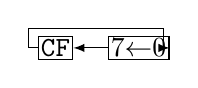
\begin{tikzpicture}[
			framed/.style={ rectangle, draw=black, inner sep=1 },
			arrow/.style={thin,->,-latex}]

			\node[framed] (cf) {\tt CF};
			\node[framed] (bits) at([xshift=3em]cf) {7$\leftarrow$0};
			\IfEqCase{#1} {
				{0}{}
				{}{\node(reg) at([yshift=-1em]bits) {\tt #2};}
			}

			\draw[arrow] (bits) -- (cf);
			\draw[arrow] (cf.west) |- +(-0.12,0) |- +(1.6,0.25) |- (bits.east);
		\end{tikzpicture}
	}
}

\newcommand{\SymRLC}[2][]{
	\SymDrawing{
		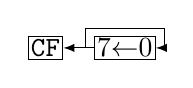
\begin{tikzpicture}[
			framed/.style={rectangle, draw=black, inner sep=1},
			arrow/.style={thin,->,-latex}]
				
			\node[framed] (cf) {\tt CF};
			\node[framed, right=1.1em of cf] (bits) {7$\leftarrow$0};
			\IfEqCase{#1} {
				{0}{}
				{}{\node[below=-1pt of bits](reg) {\tt #2};}
			}
				
			\draw[arrow] (bits) -- (cf);
			\draw[arrow] (bits.west) |- +(-0.1,0) |- +(0.9,0.25) |- (bits.east);
		\end{tikzpicture}
	}
}

\newcommand{\SymRLCu}[3][]{
	\IfEqCase{#1}{
		{0}{#2$\leftarrow$(#3+d)}
		{1}{RLC #2}
		{2}{(#3+d)$\leftarrow$#2}
		{}{\SymRLCu[0]{#2}{#3}\\\SymRLCu[1]{#2}{#3}\\\SymRLCu[2]{#2}{#3}}
	}
}

\newcommand{\SymRLD}{
	\SymDrawing{
		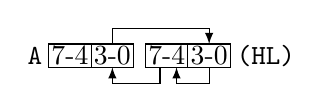
\begin{tikzpicture}[
			framed/.style={rectangle, draw=black, inner sep=1, outer sep=0},
			plain/.style={inner sep=0},
			arrow/.style={thin,->,-latex}]
			
			\node[plain] (a) {\tt A};
			
			\node[framed, right=0.5ex of a] (bitsAhi) {7-4};
			\node[framed, right=0ex of bitsAhi] (bitsAlo) {3-0};

			\node[framed, right=1ex of bitsAlo] (bitsHLhi) {7-4};
			\node[framed, right=0ex of bitsHLhi] (bitsHLlo) {3-0};
 			
			\node[plain, right=0.5ex of bitsHLlo] (hl) {\tt (HL)};
			
			\draw[arrow] (bitsHLlo.south) |- +(-0.2,-0.2) -| (bitsHLhi.310);
			\draw[arrow] (bitsHLhi.240) |- +(-0.2,-0.2) -| (bitsAlo.south);
			\draw[arrow] (bitsAlo.north) |- +(0.2,0.2) -| (bitsHLlo.north);
		\end{tikzpicture}
	}
}

\newcommand{\SymRR}[2][]{
	\SymDrawing{
		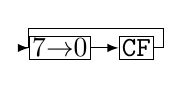
\begin{tikzpicture}[
			framed/.style={ rectangle, draw=black, inner sep=1 },
			arrow/.style={thin,->,-latex}]

			\node[framed] (bits) {7$\rightarrow$0};
			\node[framed, right=1em of bits] (cf) {\tt CF};
			\IfEqCase{#1} {
				{0}{}
				{}{\node[below=-1pt of bits](reg) {\tt #2};}
			}

			\draw[arrow] (bits) -- (cf);
			\draw[arrow] (cf.east) |- +(0.12,0) |- +(-1.6,0.25) |- (bits.west);
		\end{tikzpicture}
	}
}

\newcommand{\SymRRC}[2][]{
	\SymDrawing{
		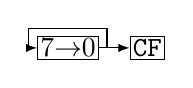
\begin{tikzpicture}[
			framed/.style={rectangle, draw=black, inner sep=1},
			arrow/.style={thin,->,-latex}]
			
			\node[framed] (bits) {7$\rightarrow$0};
			\node[framed, right=1.1em of bits] (cf) {\tt CF};
			\IfEqCase{#1} {
				{0}{}
				{}{\node[below=-1pt of bits](reg) {\tt #2};}
			}
			
			\draw[arrow] (bits) -- (cf);
			\draw[arrow] (bits.east) |- +(0.1,0) |- +(-0.9,0.25) |- (bits.west);
		\end{tikzpicture}
	}
}

\newcommand{\SymRRD}{
	\SymDrawing{
		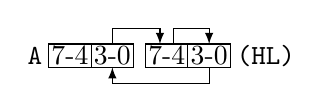
\begin{tikzpicture}[
			framed/.style={rectangle, draw=black, inner sep=1, outer sep=0},
			plain/.style={inner sep=0},
			arrow/.style={thin,->,-latex}]
			
			\node[plain] (a) {\tt A};
			
			\node[framed, right=0.5ex of a] (bitsAhi) {7-4};
			\node[framed, right=0ex of bitsAhi] (bitsAlo) {3-0};

			\node[framed, right=1ex of bitsAlo] (bitsHLhi) {7-4};
			\node[framed, right=0ex of bitsHLhi] (bitsHLlo) {3-0};
 			
			\node[plain, right=0.5ex of bitsHLlo] (hl) {\tt (HL)};
			
			\draw[arrow] (bitsHLlo.south) |- +(-0.2,-0.2) -| (bitsAlo.south);
			\draw[arrow] (bitsAlo.north) |- +(0.2,0.2) -| (bitsHLhi.120);
			\draw[arrow] (bitsHLhi.60) |- +(0.2,0.2) -| (bitsHLlo.north);
		\end{tikzpicture}
	}
}

\newcommand{\SymRST}[2][]{
	\IfEqCase{#1}{
		{0}{(SP-1)$\leftarrow$PC\High}
		{1}{(SP-2)$\leftarrow$PC\Low}
		{2}{SP$\leftarrow$SP-2}
		{3}{PC$\leftarrow$#2}
		{}{\SymRST[0]{#2}\\\SymRST[1]{#2}\\\SymRST[2]{#2}\\\SymRST[3]{#2}}
	}
}

\newcommand{\SymSET}[1]{$\mathtt{#1_b}\leftarrow$1}

\newcommand{\SymSETu}[3][]{
	\IfEqCase{#1}{
		{0}{#2$\leftarrow$(#3+d)}
		{1}{$\mathtt{#2_b}\leftarrow$1}
		{2}{(#3+d)$\leftarrow$#2}
		{}{\SymSETu[0]{#2}{#3}\\\SymSETu[1]{#2}{#3}\\\SymSETu[2]{#2}{#3}}
	}
}

\newcommand{\SymSBC}[2]{#1$\leftarrow$#1-#2-CF}

\newcommand{\SymSCF}{CF$\leftarrow$1}

\newcommand{\SymSETAE}{A$\leftarrow$unsigned(\$80)>>(E$\wedge$7)}

\newcommand{\SymSLA}[2][]{
	\SymDrawing{
		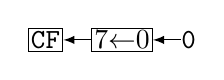
\begin{tikzpicture}[
			framed/.style={rectangle, draw=black, inner sep=1},
			plain/.style={inner sep=0},
			arrow/.style={thin,->,-latex}]

			\node[framed] (cf) {\tt CF};
			\node[framed, right=1em of cf] (bits) {7$\leftarrow$0};
			\node[plain, right=1em of bits] (zero) {\tt 0};
			\IfEqCase{#1} {
				{0}{}
				{}{\node[below=-1pt of bits](reg) {\tt #2};}
			}

			\draw[arrow] (zero) -- (bits);
			\draw[arrow] (bits) -- (cf);
		\end{tikzpicture}
	}
}

\newcommand{\SymSLI}[2][]{
	\SymDrawing{
		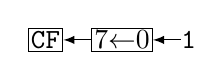
\begin{tikzpicture}[
			framed/.style={rectangle, draw=black, inner sep=1},
			plain/.style={inner sep=0},
			arrow/.style={thin,->,-latex}]

			\node[framed] (cf) {\tt CF};
			\node[framed, right=1em of cf] (bits) {7$\leftarrow$0};
			\node[plain, right=1em of bits] (one) {\tt 1};
			\IfEqCase{#1} {
				{0}{}
				{}{\node[below=-1pt of bits](reg) {\tt #2};}
			}

			\draw[arrow] (one) -- (bits);
			\draw[arrow] (bits) -- (cf);
		\end{tikzpicture}
	}
}

\newcommand{\SymSRA}[2][]{
	\SymDrawing{
		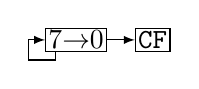
\begin{tikzpicture}[
			framed/.style={rectangle, draw=black, inner sep=1},
			arrow/.style={thin,->,-latex}]
				
			\node[framed] (bits) {7$\rightarrow$0};
			\node[framed, right=1em of bits] (cf) {\tt CF};
			\IfEqCase{#1} {
				{0}{}
				{}{\node[below=-1pt of bits](reg) {\tt #2};}
			}
				
			\draw[arrow] (bits) -- (cf);
			\draw[arrow] (bits.211) |- +(-0.35,-0.1) |- (bits.west);
		\end{tikzpicture}
	}
}

\newcommand{\SymSRL}[2][]{
	\SymDrawing{
		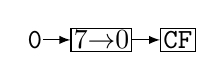
\begin{tikzpicture}[
			framed/.style={rectangle, draw=black, inner sep=1},
			plain/.style={inner sep=0},
			arrow/.style={thin,->,-latex}]
			
			\node[plain] (zero) {\tt 0};
			\node[framed, right=1em of zero] (bits) {7$\rightarrow$0};
			\node[framed, right=1em of bits] (cf) {\tt CF};
			\IfEqCase{#1} {
				{0}{}
				{}{\node[below=-1pt of bits](reg) {\tt #2};}
			}
			
			\draw[arrow] (zero) -- (bits);
			\draw[arrow] (bits) -- (cf);
		\end{tikzpicture}
	}
}

\newcommand{\SymSUB}[1]{A$\leftarrow$A-#1}

\newcommand{\SymSWAPNIB}[1][]{
	\IfEq{#1}{}{}{\hspace*{-1.6em}}
	\SymDrawing{
		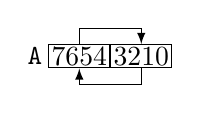
\begin{tikzpicture}[
			framed/.style={rectangle, draw=black, inner sep=1},
			plain/.style={inner sep=0},
			arrow/.style={thin,->,-latex}]
			
			\node[plain] (a) {\tt A};
			\node[framed, right=0.2em of a] (hi) {7654};
			\node[framed, right=0em of hi] (lo) {3210};
			
			\draw[arrow] (hi.north) |- +(0.1,0.2) -| (lo.north);
			\draw[arrow] (lo.south) |- +(-0.1,-0.2) -| (hi.south);
		\end{tikzpicture}
	}
}

\newcommand{\SymTEST}{A$\wedge$n}

\newcommand{\SymXOR}[1]{A$\leftarrow$A$\veebar$#1}

% ────────────────────────────────────────────────────────────────────────────
% ─██████████████─██████─────────██████████████─██████████████─██████████████─
% ─██░░░░░░░░░░██─██░░██─────────██░░░░░░░░░░██─██░░░░░░░░░░██─██░░░░░░░░░░██─
% ─██░░██████████─██░░██─────────██░░██████░░██─██░░██████████─██░░██████████─
% ─██░░██─────────██░░██─────────██░░██──██░░██─██░░██─────────██░░██─────────
% ─██░░██████████─██░░██─────────██░░██████░░██─██░░██─────────██░░██████████─
% ─██░░░░░░░░░░██─██░░██─────────██░░░░░░░░░░██─██░░██──██████─██░░░░░░░░░░██─
% ─██░░██████████─██░░██─────────██░░██████░░██─██░░██──██░░██─██████████░░██─
% ─██░░██─────────██░░██─────────██░░██──██░░██─██░░██──██░░██─────────██░░██─
% ─██░░██─────────██░░██████████─██░░██──██░░██─██░░██████░░██─██████████░░██─
% ─██░░██─────────██░░░░░░░░░░██─██░░██──██░░██─██░░░░░░░░░░██─██░░░░░░░░░░██─
% ─██████─────────██████████████─██████──██████─██████████████─██████████████─
% ────────────────────────────────────────────────────────────────────────────

% some common declarations to unify formatting of individual parts; we can then later redefine these macros to change appearance without having to tweak main macros
\newcommand{\FlagsSee}[1]{\See{#1}}		% footnote declarations
\newcommand{\FlagsFPP}{\FPP}			% PF=parity indicator
\newcommand{\FlagsFPV}{\FPV}			% PF=overflow indicator
\newcommand{\FlagsSmall}[1]{\tiny #1}	% small font size
\newcommand{\FlagsNoEffect}{}			% text for "no effect"; we don't display anything in tables, but may redeclare to display something in details section

% note: because LaTeX doesn't allow numbers in commands, we use the following notation:
% r = 8 bit register or number
% n = 8 bit number (only if we already use r)
% rr = 16 bit register pair or number
% nn = 16 bit number (only if we already use rr)
% note: we need to pass 1 optional parameter to Flags; we need it in details section
\newcommand{\FlagsADDr}[1][]{\Flags[#1]{\FS}{\FS}{\FS}{\FlagsFPV}{0}{\FS}}
\newcommand{\FlagsADDrr}[1][]{\Flags[#1]{\FN}{\FN}{\FX\FlagsSee{2}}{\FN}{0}{\FS\FlagsSee{1}}}
\newcommand{\FlagsADDrra}[1][\FlagsNoEffect]{\Flags[#1]{\FN}{\FN}{\FN}{\FN}{\FN}{\FN}}
\newcommand{\FlagsADDrrnn}[1][\FlagsNoEffect]{\Flags[#1]{\FN}{\FN}{\FN}{\FN}{\FN}{\FN}}
\newcommand{\FlagsADCr}[1][]{\Flags[#1]{\FS}{\FS}{\FS}{\FlagsFPV}{0}{\FS}}
\newcommand{\FlagsADCrr}[1][]{\Flags[#1]{\FS\FlagsSee{1}}{\FS\FlagsSee{1}}{\FX\FlagsSee{2}}{\FlagsFPV\FlagsSee{1}}{0}{\FS\FlagsSee{1}}}
\newcommand{\FlagsANDr}[1][]{\Flags[#1]{\FS}{\FS}{1}{\FlagsFPV}{0}{0}}
\newcommand{\FlagsBITr}[1][]{\Flags[#1]{\FU\FlagsSee{1}}{\FS}{1}{\FU\FlagsSee{1}}{0}{\FN}}
\newcommand{\FlagsBSLA}[1][\FlagsNoEffect]{\Flags[#1]{\FN}{\FN}{\FN}{\FN}{\FN}{\FN}}
\newcommand{\FlagsBSRA}[1][\FlagsNoEffect]{\Flags[#1]{\FN}{\FN}{\FN}{\FN}{\FN}{\FN}}
\newcommand{\FlagsBSRL}[1][\FlagsNoEffect]{\Flags[#1]{\FN}{\FN}{\FN}{\FN}{\FN}{\FN}}
\newcommand{\FlagsBSRF}[1][\FlagsNoEffect]{\Flags[#1]{\FN}{\FN}{\FN}{\FN}{\FN}{\FN}}
\newcommand{\FlagsBRLC}[1][\FlagsNoEffect]{\Flags[#1]{\FN}{\FN}{\FN}{\FN}{\FN}{\FN}}
\newcommand{\FlagsCALLnn}[1][\FlagsNoEffect]{\Flags[#1]{\FN}{\FN}{\FN}{\FN}{\FN}{\FN}}
\newcommand{\FlagsCALLccnn}[1][\FlagsNoEffect]{\Flags[#1]{\FN}{\FN}{\FN}{\FN}{\FN}{\FN}}
\newcommand{\FlagsCCF}[1][]{\Flags[#1]{\FN}{\FN}{\FX\FlagsSee{2}}{\FN}{0}{\FS}}
\newcommand{\FlagsCPr}[1][]{\Flags[#1]{\FS}{\FS}{\FS}{\FlagsFPV}{1}{\FS}}
\newcommand{\FlagsCPI}[1][]{\Flags[#1]{\FS\FlagsSee{1}}{\FX\FlagsSee{2}}{\FS\FlagsSee{1}}{\FX\FlagsSee{3}}{1}{\FN}}
\newcommand{\FlagsCPIR}[1][]{\Flags[#1]{\FS\FlagsSee{1}}{\FX\FlagsSee{2}}{\FS\FlagsSee{1}}{\FX\FlagsSee{3}}{1}{\FN}}
\newcommand{\FlagsCPD}[1][]{\Flags[#1]{\FS\FlagsSee{1}}{\FX\FlagsSee{2}}{\FS\FlagsSee{1}}{\FX\FlagsSee{3}}{1}{\FN}}
\newcommand{\FlagsCPDR}[1][]{\Flags[#1]{\FS\FlagsSee{1}}{\FX\FlagsSee{2}}{\FS\FlagsSee{1}}{\FX\FlagsSee{3}}{1}{\FN}}
\newcommand{\FlagsCPL}[1][]{\Flags[#1]{\FN}{\FN}{1}{\FN}{1}{\FN}}
\newcommand{\FlagsDAA}[1][]{\Flags[#1]{\FS}{\FS}{\FS}{\FlagsFPP}{\FN}{\FS}}
\newcommand{\FlagsDECr}[1][]{\Flags[#1]{\FS}{\FS}{\FS}{\FlagsFPV\FlagsSee{5}}{1}{\FN}}
\newcommand{\FlagsDECrr}[1][\FlagsNoEffect]{\Flags[#1]{\FN}{\FN}{\FN}{\FN}{\FN}{\FN}}
\newcommand{\FlagsDI}[1][\FlagsNoEffect]{\Flags[#1]{\FN}{\FN}{\FN}{\FN}{\FN}{\FN}}
\newcommand{\FlagsDJNZ}[1][\FlagsNoEffect]{\Flags[#1]{\FN}{\FN}{\FN}{\FN}{\FN}{\FN}}
\newcommand{\FlagsEI}[1][\FlagsNoEffect]{\Flags[#1]{\FN}{\FN}{\FN}{\FN}{\FN}{\FN}}
\newcommand{\FlagsEXrr}[1][\FlagsNoEffect]{\Flags[#1]{\FN}{\FN}{\FN}{\FN}{\FN}{\FN}}
\newcommand{\FlagsEXaf}[1][]{\Flags[#1]{\FX\FlagsSee{1}}{\FX\FlagsSee{1}}{\FX\FlagsSee{1}}{\FX\FlagsSee{1}}{\FX\FlagsSee{1}}{\FX\FlagsSee{1}}}
\newcommand{\FlagsEXX}[1][\FlagsNoEffect]{\Flags[#1]{\FN}{\FN}{\FN}{\FN}{\FN}{\FN}}
\newcommand{\FlagsHALT}[1][\FlagsNoEffect]{\Flags[#1]{\FN}{\FN}{\FN}{\FN}{\FN}{\FN}}
\newcommand{\FlagsIM}[1][\FlagsNoEffect]{\Flags[#1]{\FN}{\FN}{\FN}{\FN}{\FN}{\FN}}
\newcommand{\FlagsINan}[1][\FlagsNoEffect]{\Flags[#1]{\FN}{\FN}{\FN}{\FN}{\FN}{\FN}}
\newcommand{\FlagsINrc}[1][]{\Flags[#1]{\FS}{\FS}{0}{\FlagsFPP}{0}{\FN}}
\newcommand{\FlagsINc}[1][]{\Flags[#1]{\FS}{\FS}{0}{\FlagsFPP}{0}{\FN}}
\newcommand{\FlagsINCr}[1][]{\Flags[#1]{\FS}{\FS}{\FS}{\FlagsFPV\FlagsSee{4}}{0}{\FN}}
\newcommand{\FlagsINCrr}[1][\FlagsNoEffect]{\Flags[#1]{\FN}{\FN}{\FN}{\FN}{\FN}{\FN}}
\newcommand{\FlagsINI}[1][]{\Flags[#1]{\FX\FlagsSee{5}}{\FX\FlagsSee{4}}{\FX\FlagsSee{5}}{\FX\FlagsSee{5}}{1}{\FN}}
\newcommand{\FlagsINIR}[1][]{\Flags[#1]{\FX\FlagsSee{5}}{1}{\FX\FlagsSee{5}}{\FX\FlagsSee{5}}{1}{\FN}}
\newcommand{\FlagsIND}[1][]{\Flags[#1]{\FX\FlagsSee{5}}{\FX\FlagsSee{4}}{\FX\FlagsSee{5}}{\FX\FlagsSee{5}}{1}{\FN}}
\newcommand{\FlagsINDR}[1][]{\Flags[#1]{\FX\FlagsSee{5}}{1}{\FX\FlagsSee{5}}{\FX\FlagsSee{5}}{1}{\FN}}
\newcommand{\FlagsJPc}[1][]{\Flags[#1]{\FU}{\FU}{\FU}{\FU}{\FU}{\FU}}
\newcommand{\FlagsJPnn}[1][\FlagsNoEffect]{\Flags[#1]{\FN}{\FN}{\FN}{\FN}{\FN}{\FN}}
\newcommand{\FlagsJPccnn}[1][\FlagsNoEffect]{\Flags[#1]{\FN}{\FN}{\FN}{\FN}{\FN}{\FN}}
\newcommand{\FlagsJPrr}[1][\FlagsNoEffect]{\Flags[#1]{\FN}{\FN}{\FN}{\FN}{\FN}{\FN}}
\newcommand{\FlagsJRn}[1][\FlagsNoEffect]{\Flags[#1]{\FN}{\FN}{\FN}{\FN}{\FN}{\FN}}
\newcommand{\FlagsJRccn}[1][\FlagsNoEffect]{\Flags[#1]{\FN}{\FN}{\FN}{\FN}{\FN}{\FN}}
\newcommand{\FlagsLDr}[1][\FlagsNoEffect]{\Flags[#1]{\FN}{\FN}{\FN}{\FN}{\FN}{\FN}}
\newcommand{\FlagsLDrr}[1][\FlagsNoEffect]{\Flags[#1]{\FN}{\FN}{\FN}{\FN}{\FN}{\FN}}
\newcommand{\FlagsLDair}[1][]{\Flags[#1]{\FS}{\FS}{0}{{\FlagsSmall IFF2}}{0}{\FN}}
\newcommand{\FlagsLDI}[1][]{\Flags[#1]{\FN}{\FN}{0}{\FX\FlagsSee{3}}{0}{\FN}}
\newcommand{\FlagsLDIR}[1][]{\Flags[#1]{\FN}{\FN}{0}{0\FlagsSee{4}}{0}{\FN}}
\newcommand{\FlagsLDD}[1][]{\Flags[#1]{\FN}{\FN}{0}{\FX\FlagsSee{3}}{0}{\FN}}
\newcommand{\FlagsLDDR}[1][]{\Flags[#1]{\FN}{\FN}{0}{0\FlagsSee{4}}{0}{\FN}}
\newcommand{\FlagsLDDX}[1][\FlagsNoEffect]{\Flags[#1]{\FN}{\FN}{\FN}{\FN}{\FN}{\FN}}
\newcommand{\FlagsLDDRX}[1][\FlagsNoEffect]{\Flags[#1]{\FN}{\FN}{\FN}{\FN}{\FN}{\FN}}
\newcommand{\FlagsLDIX}[1][\FlagsNoEffect]{\Flags[#1]{\FN}{\FN}{\FN}{\FN}{\FN}{\FN}}
\newcommand{\FlagsLDIRX}[1][\FlagsNoEffect]{\Flags[#1]{\FN}{\FN}{\FN}{\FN}{\FN}{\FN}}
\newcommand{\FlagsLDPIRX}[1][\FlagsNoEffect]{\Flags[#1]{\FN}{\FN}{\FN}{\FN}{\FN}{\FN}}
\newcommand{\FlagsLDWS}[1][]{\Flags[#1]{\FS}{\FS}{\FS}{\FlagsFPV\FlagsSee{2}}{0}{\FN}}
\newcommand{\FlagsMIRRORa}[1][\FlagsNoEffect]{\Flags[#1]{\FN}{\FN}{\FN}{\FN}{\FN}{\FN}}
\newcommand{\FlagsMULde}[1][\FlagsNoEffect]{\Flags[#1]{\FN}{\FN}{\FN}{\FN}{\FN}{\FN}}
\newcommand{\FlagsNEG}[1][]{\Flags[#1]{\FS}{\FS}{\FS}{\FlagsFPP}{1}{\FS}}
\newcommand{\FlagsNEXTREGna}[1][\FlagsNoEffect]{\Flags[#1]{\FN}{\FN}{\FN}{\FN}{\FN}{\FN}}
\newcommand{\FlagsNEXTREGnn}[1][\FlagsNoEffect]{\Flags[#1]{\FN}{\FN}{\FN}{\FN}{\FN}{\FN}}
\newcommand{\FlagsNOP}[1][\FlagsNoEffect]{\Flags[#1]{\FN}{\FN}{\FN}{\FN}{\FN}{\FN}}
\newcommand{\FlagsORr}[1][]{\Flags[#1]{\FS}{\FS}{0}{\FlagsFPV}{0}{0}}
\newcommand{\FlagsOUTna}[1][\FlagsNoEffect]{\Flags[#1]{\FN}{\FN}{\FN}{\FN}{\FN}{\FN}}
\newcommand{\FlagsOUTcr}[1][\FlagsNoEffect]{\Flags[#1]{\FN}{\FN}{\FN}{\FN}{\FN}{\FN}}
\newcommand{\FlagsOUTc}[1][\FlagsNoEffect]{\Flags[#1]{\FN}{\FN}{\FN}{\FN}{\FN}{\FN}}
\newcommand{\FlagsOUTI}[1][]{\Flags[#1]{\FX\FlagsSee{2}}{\FX\FlagsSee{1}}{\FX\FlagsSee{2}}{\FX\FlagsSee{2}}{1}{\FN}}
\newcommand{\FlagsOTIR}[1][]{\Flags[#1]{\FX\FlagsSee{2}}{1}{\FX\FlagsSee{2}}{\FX\FlagsSee{2}}{1}{\FN}}
\newcommand{\FlagsOUTD}[1][]{\Flags[#1]{\FX\FlagsSee{2}}{\FX\FlagsSee{1}}{\FX\FlagsSee{2}}{\FX\FlagsSee{2}}{1}{\FN}}
\newcommand{\FlagsOTDR}[1][]{\Flags[#1]{\FX\FlagsSee{2}}{1}{\FX\FlagsSee{2}}{\FX\FlagsSee{2}}{1}{\FN}}
\newcommand{\FlagsOUTINB}[1][]{\Flags[#1]{\FU}{\FU}{\FU}{\FU}{\FU}{\FU}}
\newcommand{\FlagsPIXELAD}[1][\FlagsNoEffect]{\Flags[#1]{\FN}{\FN}{\FN}{\FN}{\FN}{\FN}}
\newcommand{\FlagsPIXELDN}[1][\FlagsNoEffect]{\Flags[#1]{\FN}{\FN}{\FN}{\FN}{\FN}{\FN}}
\newcommand{\FlagsPOPrr}[1][\FlagsNoEffect]{\Flags[#1]{\FN}{\FN}{\FN}{\FN}{\FN}{\FN}}
\newcommand{\FlagsPOPaf}[1][]{\Flags[#1]{\FS\FlagsSee{1}}{\FS\FlagsSee{1}}{\FS\FlagsSee{1}}{\FS\FlagsSee{1}}{\FS\FlagsSee{1}}{\FS\FlagsSee{1}}}
\newcommand{\FlagsPUSHrr}[1][\FlagsNoEffect]{\Flags[#1]{\FN}{\FN}{\FN}{\FN}{\FN}{\FN}}
\newcommand{\FlagsPUSHnn}[1][\FlagsNoEffect]{\Flags[#1]{\FN}{\FN}{\FN}{\FN}{\FN}{\FN}}
\newcommand{\FlagsRESr}[1][\FlagsNoEffect]{\Flags[#1]{\FN}{\FN}{\FN}{\FN}{\FN}{\FN}}
\newcommand{\FlagsRET}[1][\FlagsNoEffect]{\Flags[#1]{\FN}{\FN}{\FN}{\FN}{\FN}{\FN}}
\newcommand{\FlagsRETcc}[1][\FlagsNoEffect]{\Flags[#1]{\FN}{\FN}{\FN}{\FN}{\FN}{\FN}}
\newcommand{\FlagsRETI}[1][\FlagsNoEffect]{\Flags[#1]{\FN}{\FN}{\FN}{\FN}{\FN}{\FN}}
\newcommand{\FlagsRETN}[1][\FlagsNoEffect]{\Flags[#1]{\FN}{\FN}{\FN}{\FN}{\FN}{\FN}}
\newcommand{\FlagsRLr}[1][]{\Flags[#1]{\FS}{\FS}{0}{\FlagsFPP}{0}{\FS}}
\newcommand{\FlagsRLA}[1][]{\Flags[#1]{\FN}{\FN}{0}{\FN}{0}{\FS}}
\newcommand{\FlagsRLCr}[1][]{\Flags[#1]{\FS}{\FS}{0}{\FlagsFPP}{0}{\FS}}
\newcommand{\FlagsRLCA}[1][]{\Flags[#1]{\FN}{\FN}{0}{\FN}{0}{\FS}}
\newcommand{\FlagsRLD}[1][]{\Flags[#1]{\FS}{\FS}{0}{\FlagsFPP}{0}{\FN}}
\newcommand{\FlagsRRr}[1][]{\Flags[#1]{\FS}{\FS}{0}{\FlagsFPP}{0}{\FS}}
\newcommand{\FlagsRRA}[1][]{\Flags[#1]{\FN}{\FN}{0}{\FN}{0}{\FS}}
\newcommand{\FlagsRRCr}[1][]{\Flags[#1]{\FS}{\FS}{0}{\FlagsFPP}{0}{\FS}}
\newcommand{\FlagsRRCA}[1][]{\Flags[#1]{\FN}{\FN}{0}{\FN}{0}{\FS}}
\newcommand{\FlagsRRD}[1][]{\Flags[#1]{\FS}{\FS}{0}{\FlagsFPP}{0}{\FN}}
\newcommand{\FlagsRSTn}[1][\FlagsNoEffect]{\Flags[#1]{\FN}{\FN}{\FN}{\FN}{\FN}{\FN}}
\newcommand{\FlagsSBCr}[1][]{\Flags[#1]{\FS}{\FS}{\FS}{\FlagsFPV}{1}{\FS}}
\newcommand{\FlagsSBCrr}[1][]{\Flags[#1]{\FS\FlagsSee{1}}{\FS\FlagsSee{1}}{\FX\FlagsSee{2}}{\FlagsFPV\FlagsSee{1}}{1}{\FS\FlagsSee{1}}}
\newcommand{\FlagsSCF}[1][]{\Flags[#1]{\FN}{\FN}{0}{\FN}{0}{1}}
\newcommand{\FlagsSETr}[1][\FlagsNoEffect]{\Flags[#1]{\FN}{\FN}{\FN}{\FN}{\FN}{\FN}}
\newcommand{\FlagsSETAE}[1][\FlagsNoEffect]{\Flags[#1]{\FN}{\FN}{\FN}{\FN}{\FN}{\FN}}
\newcommand{\FlagsSLAr}[1][]{\Flags[#1]{\FS}{\FS}{0}{\FlagsFPP}{0}{\FS}}
\newcommand{\FlagsSLIr}[1][]{\Flags[#1]{\FS}{\FS}{0}{\FlagsFPP}{0}{\FS}}
\newcommand{\FlagsSRAr}[1][]{\Flags[#1]{\FS}{\FS}{0}{\FlagsFPP}{0}{\FS}}
\newcommand{\FlagsSRLr}[1][]{\Flags[#1]{\FS}{\FS}{0}{\FlagsFPP}{0}{\FS}}
\newcommand{\FlagsSUBr}[1][]{\Flags[#1]{\FS}{\FS}{\FS}{\FlagsFPV}{1}{\FS}}
\newcommand{\FlagsSWAPNIB}[1][\FlagsNoEffect]{\Flags[#1]{\FN}{\FN}{\FN}{\FN}{\FN}{\FN}}
\newcommand{\FlagsTESTn}[1][]{\Flags[#1]{\FS}{\FS}{\FS}{\FlagsFPV}{\FU}{\FS}}
\newcommand{\FlagsXORr}[1][]{\Flags[#1]{\FS}{\FS}{0}{\FlagsFPP}{0}{0}}



\begin{document}

% use arabic numerals for starting pages
\frontmatter

% TODO
% - Describe BIT A,(HL) undocumented flags from internal MEMPRT/WZ register
% - Add testing code to appendices


% ████████████████████████████████████████████████████████████████████████
% █░░░░░░░░░░░░░░█░░░░░░░░░░█░░░░░░░░░░░░░░█░░░░░░█████████░░░░░░░░░░░░░░█
% █░░▄▀▄▀▄▀▄▀▄▀░░█░░▄▀▄▀▄▀░░█░░▄▀▄▀▄▀▄▀▄▀░░█░░▄▀░░█████████░░▄▀▄▀▄▀▄▀▄▀░░█
% █░░░░░░▄▀░░░░░░█░░░░▄▀░░░░█░░░░░░▄▀░░░░░░█░░▄▀░░█████████░░▄▀░░░░░░░░░░█
% █████░░▄▀░░███████░░▄▀░░███████░░▄▀░░█████░░▄▀░░█████████░░▄▀░░█████████
% █████░░▄▀░░███████░░▄▀░░███████░░▄▀░░█████░░▄▀░░█████████░░▄▀░░░░░░░░░░█
% █████░░▄▀░░███████░░▄▀░░███████░░▄▀░░█████░░▄▀░░█████████░░▄▀▄▀▄▀▄▀▄▀░░█
% █████░░▄▀░░███████░░▄▀░░███████░░▄▀░░█████░░▄▀░░█████████░░▄▀░░░░░░░░░░█
% █████░░▄▀░░███████░░▄▀░░███████░░▄▀░░█████░░▄▀░░█████████░░▄▀░░█████████
% █████░░▄▀░░█████░░░░▄▀░░░░█████░░▄▀░░█████░░▄▀░░░░░░░░░░█░░▄▀░░░░░░░░░░█
% █████░░▄▀░░█████░░▄▀▄▀▄▀░░█████░░▄▀░░█████░░▄▀▄▀▄▀▄▀▄▀░░█░░▄▀▄▀▄▀▄▀▄▀░░█
% █████░░░░░░█████░░░░░░░░░░█████░░░░░░█████░░░░░░░░░░░░░░█░░░░░░░░░░░░░░█
% ████████████████████████████████████████████████████████████████████████


% first page should be offset to the right to accomodate the binding; default setup assumes this is odd page so sets it up the other way around (binding offset on the right side), but it gets printed as even page
\newgeometry{left=4cm,right=3cm}

\title{\BookTitle}
\author{\AuthorNameSurname}
\date{Version \LatestVersion, \today}

\maketitle

% all other after this one should use defaults from `usepackage' statement on the top of the file!
\afterpage{\aftergroup\restoregeometry}


\chapter*{Copyright Statement}

Copyright {\copyright} \LatestYear ~\AuthorNameSurname\\	% note this should become 2021-\LatestYear for releases after 2021...
Copyright {\copyright} 2005 Jan Wilmans\\
Copyright {\copyright} 1997, 1998, 2001, 2003, 2005 Sean Young

Permission is granted to copy, distribute and/or modify this document under the terms of the GNU Free Documentation License, Version 1.1 or any later version published by the Free Software Foundation; with no Invariant Sections, with no Front-Cover Texts, and with no Back-Cover Texts. A copy of the license is included in the section entitled ``GNU Free Documentation License''.



% start numbering pages with table of contents, set style to clean so page numbers will be visible and other page styles reflected
\setcounter{page}{0}
\pagestyle{clean}

% print table of contents, but just chapters and sections, we'll print toc for each chapter separately that will include subsection as well
\setcounter{tocdepth}{1}
\dominitoc \tableofcontents

% setup formatting for section toc - no horizontal delimiters, offsets etc.
\noptcrule
\nomtcrule									% no horizontal delimiters on top and bottom
\renewcommand{\mtcoffset}{-1.5em}			% render minitoc a bit more to the left for more centralized appearance
\mtcsetfeature{minitoc}{open}{\vspace{1em}}	% add some vertical spacing between contents title and toc
\def\mtcSfont{\normalsize}
\def\mtcSSfont{\small}



% use arabic numerals for page numbers and clean page style for the rest of the document
\mainmatter


\chapter{Introduction}

% ████████████████████████████████████████████████████████████████████████████████████
% █░░░░░░░░░░█░░░░░░██████████░░░░░░█░░░░░░░░░░░░░░█░░░░░░░░░░░░░░░░███░░░░░░░░░░░░░░█
% █░░▄▀▄▀▄▀░░█░░▄▀░░░░░░░░░░██░░▄▀░░█░░▄▀▄▀▄▀▄▀▄▀░░█░░▄▀▄▀▄▀▄▀▄▀▄▀░░███░░▄▀▄▀▄▀▄▀▄▀░░█
% █░░░░▄▀░░░░█░░▄▀▄▀▄▀▄▀▄▀░░██░░▄▀░░█░░░░░░▄▀░░░░░░█░░▄▀░░░░░░░░▄▀░░███░░▄▀░░░░░░▄▀░░█
% ███░░▄▀░░███░░▄▀░░░░░░▄▀░░██░░▄▀░░█████░░▄▀░░█████░░▄▀░░████░░▄▀░░███░░▄▀░░██░░▄▀░░█
% ███░░▄▀░░███░░▄▀░░██░░▄▀░░██░░▄▀░░█████░░▄▀░░█████░░▄▀░░░░░░░░▄▀░░███░░▄▀░░██░░▄▀░░█
% ███░░▄▀░░███░░▄▀░░██░░▄▀░░██░░▄▀░░█████░░▄▀░░█████░░▄▀▄▀▄▀▄▀▄▀▄▀░░███░░▄▀░░██░░▄▀░░█
% ███░░▄▀░░███░░▄▀░░██░░▄▀░░██░░▄▀░░█████░░▄▀░░█████░░▄▀░░░░░░▄▀░░░░███░░▄▀░░██░░▄▀░░█
% ███░░▄▀░░███░░▄▀░░██░░▄▀░░░░░░▄▀░░█████░░▄▀░░█████░░▄▀░░██░░▄▀░░█████░░▄▀░░██░░▄▀░░█
% █░░░░▄▀░░░░█░░▄▀░░██░░▄▀▄▀▄▀▄▀▄▀░░█████░░▄▀░░█████░░▄▀░░██░░▄▀░░░░░░█░░▄▀░░░░░░▄▀░░█
% █░░▄▀▄▀▄▀░░█░░▄▀░░██░░░░░░░░░░▄▀░░█████░░▄▀░░█████░░▄▀░░██░░▄▀▄▀▄▀░░█░░▄▀▄▀▄▀▄▀▄▀░░█
% █░░░░░░░░░░█░░░░░░██████████░░░░░░█████░░░░░░█████░░░░░░██░░░░░░░░░░█░░░░░░░░░░░░░░█
% ████████████████████████████████████████████████████████████████████████████████████

\minitoc


\section{Where to get this document}

\BookTitle ~is available as coil bound printed book on

\url{https://bit.ly/zx-next-assembler-dev-guide}

You can also download it as PDF document from github where you can also find its source \LaTeX ~form so you can edit it to your preference

\url{https://github.com/tomaz/zx-next-dev-guide}


\section{Companion Source Code}

github repository also includes companion source code. Sample projects were created in cross platform environment on Windows so instructions here are written with these in mind. But consider them merely as suggestion; you should be able to use your preferred editor or tools.

\pagebreak % we want list of all tools and software to be on the same page
\begin{description}[style=unboxed,leftmargin=0cm]
	\item[Visual Studio Code (\url{https://code.visualstudio.com/})]\hfill
	
	My code editor of choice! I use it with the following plugins:

	\begin{description}[topsep=1pt,labelindent=2em,leftmargin=2em]
		\item[DeZog plugin (\url{https://github.com/maziac/DeZog})]\hfill
	
		Essential plugin; features list is too large to even attempt to enumerate here, but essentially turns VS Code into fully fledged debugging environment.

		\item[Z80 Macro-Assembler (\url{https://github.com/mborik/z80-macroasm-vscode})]\hfill
		
		Another must-have plugin for Z80 assembly developer; syntax highlighting, code formatting and code completion, renaming etc.

		\item[Z80 Instruction Set (\url{https://github.com/maziac/z80-instruction-set})]\hfill
		
		Adds mouse hover action above any Z80N instruction for quick info.

		\item[Z80 Assembly meter (\url{https://github.com/theNestruo/z80-asm-meter-vscode})]\hfill
		
		Shows the sum of clock cycles and machine code bytes for all instructions in current selection.
	\end{description}
	
	\item[sjasmplus 1.18.2 (\url{https://github.com/z00m128/sjasmplus})]\hfill

	Source code includes sjasmplus specific directives for creating nex files at top and bottom of {\tt main.asm} files; if you use different compiler, you may need to tweak or comment them out.

	VS Code projects are setup to expect binaries in specific folder. You will need to download and copy so that {\tt sjasmplus.exe} is located in {\tt Tools/sjasmplus}.

	\item[CSpect 2.13.0 (\url{http://cspect.org})]\hfill

	Similar to sjasmplus, CSpect binaries are expected in specific folder. To install, download and copy so that {\tt CSpect.exe} is located in {\tt Tools/CSpect} folder.

	\item[CSpect Next Image (\url{http://www.zxspectrumnext.online/#sd})]\hfill

	You will also need to download ZX Spectrum Next image file and copy it to the folder where {\tt CSpect.exe} is located. I use 2GB image, hence VS Code project file is configured for that. If you use different image, make sure to update {\tt .vscode/tasks.json} file.
	
	\item[DeZog CSpect plugin (\url{https://github.com/maziac/DeZogPlugin})]\hfill

	DeZog requires this plugin to be installed in order to work with CSpect. To install, download and copy to the same folder where {\tt CSpect.exe} is located. Make sure plugin version matches DeZog version!

\end{description}

{
	\footnotesize

	\begin{description}[topsep=1pt,itemsep=1pt,labelindent=0pt,leftmargin=0pt]		
		\item[Note:] you need to have CSpect launched before you can run the samples. I created couple tasks\footnotemark~for it: open VS Code command palette ({\tt Ctrl+Shift+P} shortcut on my installation) and select \textit{Tasks: Run Task} option, then select \textit{Launch CSpect} from list. This is only needed once, afterwards use \textit{Run \textgreater ~Start Debugging} from main menu to compile and launch the program.

		\item[Note:] default DeZog port of 11000 doesn't work on my computer, so I changed it to 13000. This needs to be managed in 2 places: {\tt .vscode/launch.json} and on plugin side. Companion code repository already includes the setup needed, including {\tt DeZogPlugin.dll.config} file, so it should work out of the box.
	
		\item[Note:] sample projects are ready for ZEsarUX as well, select the option from debug panel in VS Code.
	\end{description}
}

\footnotetext{
	Unfortunately with latest VS Code versions, workspace tasks stopped working. However there is a workaround: open {\tt .vscode/tasks.json} file from any of the sample projects, scroll down a little and copy {\tt Launch CSpect} and {\tt Launch ZEsarUX} tasks to user tasks. You can do this all from within VS Code. To open user tasks file, open command palette and start typing {\tt open user tasks}, then select the option from drop down menu.
}


\pagebreak % we want next section to be on its own page, fully visible when listing physical book
\section{Background, Contact \& Feedback}

My first computer was ZX Spectrum 48K. Initially it was only used to play games, but my creative mind soon set me on the path of building simple games of my own in BASIC. While too young to master assembler at that point, the idea stayed with me. ZX Spectrum Next revived my wish to learn Z80 and return to writing games for the platform.
	
My original intent was to have coil bound list of all ZX Next instructions so I can quickly compare. However after finding Z80 Undocumented online, it felt like a perfect starting point. And with additional information it included, it also encouraged me to extend mere instructions list with Next specific chapters. So in a way this book represents my notes as I was learning those topics. That being said, I did my best to present information as a reference to keep book relevant.

English is not my native tounge. And our own mind is not the best tool to correct our own work either. Since I can't afford professional proofreader, mistakes are a matter of fact I'm afraid. If you spot something, or want to contribute, feel free to open an issue on github. Pull requests are also welcome! If you want to contribute, but are unsure of what, check accompanying readme file on github for ideas. If you want to discuss in advance, or for anything else, you can find me on email \email{tkragelj}{gmail}{com} or Twitter {\tt @tomsbarks}.

That being said, I hope you'll enjoy reading this document as much as I did writting it!

Sincerely, \AuthorName


\pagebreak
\section{Z80 Undocumented}

As the saying ``standing on the shoulders of giants'' goes, this book is also based on pre-existing work from Jan and Sean. While my work is ZX Spectrum Next developer oriented, their original project was more focused on hardware perspective, for Z80 emulator developer.

If interested, you can find it at \url{http://www.myquest.nl/z80undocumented/}.

\begin{description}[style=unboxed,leftmargin=0cm]
	\item[Jan]\hfill
	
	\url{http://www.myquest.nl/z80undocumented/}\\
	Email \email{jw}{dds}{nl}\\
	Twitter {\tt @janwilmans}

	Interested in emulation for a long time, but a few years after Sean started writing this document, I have also started writing my own MSX emulator in 2003 and I've used this document quite a lot. Now (2005) the Z80 emulation is nearing perfection, I decided to add what extra I have learned and comments various people have sent to Sean, to this document.

	I have restyled the document (although very little) to fit my personal needs and I have checked a lot of things that were already in here.
 
	\item[Sean]\hfill

	\url{http://www.msxnet.org/}
	
	Ever since I first started working on an MSX emulator, I've been very interested in getting the emulation absolutely correct - including the undocumented features. Not just to make sure that all games work, but also to make sure that if a program crashes, it crashes exactly the same way if running on an emulator as on the real thing. Only then is perfection achieved.

	I set about collecting information. I found pieces of information on the Internet, but not everything there is to know. So I tried to fill in the gaps, the results of which I put on my website. Various people have helped since then; this is the result of all those efforts and to my knowledge this document is the most complete.
\end{description}


\pagebreak
\section{ChangeLog}

\begin{description}

	\item[11th May 2021 (Version 1.0)]
	Added ZX Spectrum Next information and instructions and restructured text for better maintainability and readability.

	\item[18th September 2005 (version 0.91)]
	Corrected a textual typo in the R register and memory refresh section, thanks to David Aubespin. Corrected the contradiction in the {\tt DAA} section saying the {\tt NF} flag was both affected and unchanged :) thanks to Dan Meir.Added an error in official documentation about that way Interrupt Mode 2 works, thanks to Aaldert Dekker.
	
	\item[15th Juni 2005 (version 0.9)]
	Corrected improper notation of {\tt JP x,nn} mnemonics in opcode list, thanks to Laurens Holst. Corrected a mistake in the {\tt INI}, {\tt INIR}, {\tt IND}, {\tt INDR} section and documented a mistake in offical Z80 documentation concerning Interrupt Mode 2, thanks to Boris Donko. Thanks to Aaldert Dekker for his ideas, for verifying many assumptions and writing instruction exercisers for various instruction groups.

	\item[18th May 2005 (version 0.8)]
	Added an alphabetical list of instructions for easy reference and corrected an error in the 16-bit arithmetic section, {\tt SBC HL,nn} sets the NF flag just like other subtraction instructions, thanks to Fredrik Olssen for pointing that out.

	\item[4th April 2005 (version 0.7)]
	I (Jan \email{jw}{dds}{nl}) will be maintaining this document from this version on. I restyled the document to fix the page numbering issues, corrected an error in the I/O Block Instructions section, added graphics for the {\tt RLD} and {\tt RRD} instructions and corrected the spelling in several places.

	\item[20th November 2003 (version 0.6)]
	Again, thanks to Ramsoft, added PV flag to {\tt OUTI}, {\tt INI} and friends. Minor fix to {\tt DAA} tables, other minor fixes.

	\item[13th November 2003 (version 0.5)]
	Thanks to Ramsoft, add the correct tables for the {\tt DAA} instruction (section \ref{daa}). Minor corrections \& typos, thanks to Jim Battle, David Sutherland and most of all Fred Limouzin.

	\item[September 2001 (version 0.4)]
	Previous documents I had written were in plain text and Microsoft Word, which I now find very embarrassing, so I decided to combine them all and use {\LaTeX}. Apart from a full re-write, the only changed information is ``Power on defaults'' (section \ref{pon}) and the algorithm for the CF and HF flags for {\tt OTIR} and friends (section \ref{block_io}).

\end{description}



\pagebreak
\IntentionallyEmpty
\pagebreak


\chapter{Zilog Z80}

% ██████████████████████████████████████████████████
% █░░░░░░░░░░░░░░░░░░█░░░░░░░░░░░░░░█░░░░░░░░░░░░░░█
% █░░▄▀▄▀▄▀▄▀▄▀▄▀▄▀░░█░░▄▀▄▀▄▀▄▀▄▀░░█░░▄▀▄▀▄▀▄▀▄▀░░█
% █░░░░░░░░░░░░▄▀▄▀░░█░░▄▀░░░░░░▄▀░░█░░▄▀░░░░░░▄▀░░█
% █████████░░░░▄▀░░░░█░░▄▀░░██░░▄▀░░█░░▄▀░░██░░▄▀░░█
% ███████░░░░▄▀░░░░███░░▄▀░░░░░░▄▀░░█░░▄▀░░██░░▄▀░░█
% █████░░░░▄▀░░░░█████░░▄▀▄▀▄▀▄▀▄▀░░█░░▄▀░░██░░▄▀░░█
% ███░░░░▄▀░░░░███████░░▄▀░░░░░░▄▀░░█░░▄▀░░██░░▄▀░░█
% █░░░░▄▀░░░░█████████░░▄▀░░██░░▄▀░░█░░▄▀░░██░░▄▀░░█
% █░░▄▀▄▀░░░░░░░░░░░░█░░▄▀░░░░░░▄▀░░█░░▄▀░░░░░░▄▀░░█
% █░░▄▀▄▀▄▀▄▀▄▀▄▀▄▀░░█░░▄▀▄▀▄▀▄▀▄▀░░█░░▄▀▄▀▄▀▄▀▄▀░░█
% █░░░░░░░░░░░░░░░░░░█░░░░░░░░░░░░░░█░░░░░░░░░░░░░░█
% ██████████████████████████████████████████████████

\minitoc

\pagebreak
\section{Overview}
\subsection{History of the Z80}

In 1969 Intel was approached by a Japanese company called Busicom to produce  chips for Busicom's electronic desktop calculator. Intel suggested that the calculator should be built around a single-chip generalized computing engine and thus was born the first microprocessor - the 4004. Although it was based on ideas from much larger mainframe and mini-computers the 4004 was cut down to fit onto a 16-pin chip, the largest that was available at the time, so that its data bus and address bus were each only 4-bits wide. 

Intel went on to improve the design and produced the 4040 (an improved 4-bit design) the 8008 (the first 8-bit microprocessor) and then in 1974 the 8080. This last one turned out to be a very useful and popular design and was used in the first home computer, the Altair 8800, and CP/M. 

In 1975 Federico Faggin who had had worked at Intel on the 4004 and its successors left the company and joined forces with Masatoshi Shima to from Zilog. At their new company Faggin and Shima designed a microprocessor that was compatible with Intel's 8080 (it ran all 78 instructions of the 8080 in almost the same way that Intel's chip did)\footnote{Thanks to Jim Battle (\email{frustum}{pacbell}{net}): the 8080 always puts the parity in the PF flag; VF does not exist and the timing is different. Possibly there are other differences.} but had many more abilities (an extra 120 instructions, many more registers, simplified connection to hardware). Thus was born the mighty Z80, and thus was the empire forged!

The original Z80 was first released in July 1976, coincidentally Jan was born in the very same month. Since then newer versions have appeared with much of the same architecture but running at higher speeds. The original Z80 ran with a clock rate of 2.5MHz, the Z80A runs at 4MHz, the Z80B at 6MHz and the Z80H at 8Mhz. 

Many companies produced machines based around Zilog's improved chip during the 1970's and 80's and because the chip could run 8080 code without needing any changes to the code the perfect choice of operating system was CP/M. 

Also Zilog has created a Z280, an enhanced version of the Zilog Z80 with a 16 bit architecture, introduced in July, 1987. It added an MMU to expand addressing to 16Mb, features for multitasking, a 256 byte cache, and a huge number of new opcodes (giving a total of over 2000!). Its internal clock runs at 2 or 4 times the external clock (e.g. a 16MHz CPU with a 4MHz bus.

The Z380 CPU incorporates advanced architectural while maintaining Z80/Z180 object code compatibility. The Z380 CPU is an enhanced version of the Z80 CPU. The Z80 instruction set has been retained, adding a full complement of 16-bit arithmetic and logical operations, multiply and divide, a complete set of register-to-register loads and exchanges, plus 32-bit load and exchange, and 32-bit arithmetic operations for address calculations.

The addressing modes of the Z80 have been enhanced with Stack pointer relative loads and stores, 16-bit and 24-bit indexed offsets and more flexible indirect register addressing. All of the addressing modes allow access to the entire 32-bit addressing space.


\subsection{Registers}

The following accessible registers exist in the Z80.

\newcommand{\RegDesc}[2]{\rdelim\}{#1}{1ex}[#2]}

\begin{tabular}{|c|c|l}
	\cline{1-2}
	\tt A & \tt F & \} Accumulator and Flags \\
	\cline{1-2}
	\multicolumn{2}{|c|}{\tt BC} & \RegDesc{3}{General purpose registers} \\ 
	\cline{1-2}
	\multicolumn{2}{|c|}{\tt DE} & \\ 
	\cline{1-2}
	\multicolumn{2}{|c|}{\tt HL} & \\ 
	\cline{1-2}
	\multicolumn{2}{|c|}{\tt IX} & \RegDesc{2}{Index registers} \\ 
	\cline{1-2}
	\multicolumn{2}{|c|}{\tt IY} & \\ 
	\cline{1-2}
	\multicolumn{2}{|c|}{\tt PC} & \RegDesc{3}{Special purpose registers} \\ 
	\cline{1-2}
	\multicolumn{2}{|c|}{\tt SP} & \\ 
	\cline{1-2}
	\tt I & \tt R & \\
	\cline{1-2}
	\multicolumn{2}{|c|}{\tt AF'} & \RegDesc{4}{Alternate general purpose registers} \\ 
	\cline{1-2}
	\multicolumn{2}{|c|}{\tt BC'} & \\ 
	\cline{1-2}
	\multicolumn{2}{|c|}{\tt DE'} & \\ 
	\cline{1-2}
	\multicolumn{2}{|c|}{\tt HL'} & \\ 
	\cline{1-2}
\end{tabular}


\subsection{Flags}
\label{flags}

The conventional way of denoting the flags is with one letter, ``C'' for the carry flag for example. It could be confused with the C register, so I've chosen to use the ``CF'' notation for flags (except ``P'' which uses ``PV'' notation due to having dual purpose, either as parity or overflow). And for YF and XF the same notation used in MAME\footnote{\url{http://www.mame.net/}}.

\begin{tabular}{|l|c|c|c|c|c|c|c|c|} 
	\hline
	bit & 7 & 6 & 5 & 4 & 3 & 2 & 1 & 0 \instrt\instrb \\
	\hline
	flag & SF & ZF & YF & HF & XF & PF & NF & CF \instrt\instrb \\ 
	\hline
\end{tabular}

\begin{description}

	\item[SF]
	Set if the 2-complement value is negative; simply a copy of the most significant bit.

	\item[ZF]
	Set if the result is zero.

	\item[YF]
	A copy of bit 5 of the result.

	\item[HF]
	The half-carry of an addition/subtraction (from bit 3 to 4). Needed for BCD correction with {\tt DAA}.

	\item[XF]
	A copy of bit 3 of the result.

	\item[PV]
	This flag can either be the parity of the result (PF), or the 2-complement signed overflow (VF): set if 2-complement value doesn't fit in the register.

	\item[NF]
	Shows whether the last operation was an addition (0) or a subtraction (1). This information is needed for {\tt DAA}.\footnote{Wouldn't it be better to have separate instructions for {\tt DAA} after addition and subtraction, like the 80x86 has instead of sacrificing a bit in the flag register?}

	\item[CF]
	The carry flag, set if there was a carry after the most significant bit.

\end{description}


\subsection{Pin Descriptions \cite{datasheet}}

This section might be relevant even if you don't do anything with hardware; it might give you insight into how the Z80 operates. Besides, it took me hours to draw this.

{\tt 
	\setlength{\unitlength}{1mm}
	\begin{picture}(50,80)
		\multiput(11.8,2)(0,3.9){20}{\framebox(2,2){}}
		\multiput(36.2,2)(0,3.9){20}{\framebox(2,2){}}
		\thicklines \footnotesize
		\put(14,0){\framebox(22,80){Z80 CPU}}
		\put(25,80){\oval(3,3)[b]}
		\thinlines 
		\newcounter{pinno}
		\multiput(15,76)(0,-3.9){20}{\stepcounter{pinno}\makebox(2,2){\arabic{pinno}}}
		\multiput(33,2)(0,3.9){20}{\stepcounter{pinno}\makebox(2,2)[r]{\arabic{pinno}}}

		\put(9,2){\makebox(2,2)[r]{$\mathtt{\overline{IORQ}}$}}
		\put(9,5.9){\makebox(2,2)[r]{$\mathtt{\overline{MREQ}}$}}
		\put(9,9.8){\makebox(2,2)[r]{$\mathtt{\overline{HALT}}$}}
		\put(9,13.7){\makebox(2,2)[r]{$\mathtt{\overline{NMI}}$}}
		\put(9,17.6){\makebox(2,2)[r]{$\mathtt{\overline{INT}}$}}
		\put(9,21.5){\makebox(2,2)[r]{$\mathtt{D_1}$}}
		\put(9,25.4){\makebox(2,2)[r]{$\mathtt{D_0}$}}
		\put(9,29.3){\makebox(2,2)[r]{$\mathtt{D_7}$}}
		\put(9,33.2){\makebox(2,2)[r]{$\mathtt{D_2}$}}
		\put(9,37.1){\makebox(2,2)[r]{$\mathtt{+ 5V}$}}
		\put(9,41){\makebox(2,2)[r]{$\mathtt{D_6}$}}
		\put(9,44.9){\makebox(2,2)[r]{$\mathtt{D_5}$}}
		\put(9,48.8){\makebox(2,2)[r]{$\mathtt{D_3}$}}
		\put(9,52.7){\makebox(2,2)[r]{$\mathtt{D_4}$}}
		\put(9,56.6){\makebox(2,2)[r]{$\mathtt{CLK}$}}
		\put(9,60.5){\makebox(2,2)[r]{$\mathtt{A_{15}}$}}
		\put(9,64.4){\makebox(2,2)[r]{$\mathtt{A_{14}}$}}
		\put(9,68.3){\makebox(2,2)[r]{$\mathtt{A_{13}}$}}
		\put(9,72.2){\makebox(2,2)[r]{$\mathtt{A_{12}}$}}
		\put(9,76.1){\makebox(2,2)[r]{$\mathtt{A_{11}}$}}

		\put(39,2){\makebox(2,2)[l]{$\mathtt{\overline{RD}}$}}
		\put(39,5.9){\makebox(2,2)[l]{$\mathtt{\overline{WR}}$}}
		\put(39,9.8){\makebox(2,2)[l]{$\mathtt{\overline{BUSACK}}$}}
		\put(39,13.7){\makebox(2,2)[l]{$\mathtt{\overline{WAIT}}$}}
		\put(39,17.6){\makebox(2,2)[l]{$\mathtt{\overline{BUSREQ}}$}}
		\put(39,21.5){\makebox(2,2)[l]{$\mathtt{\overline{RESET}}$}}
		\put(39,25.4){\makebox(2,2)[l]{$\mathtt{\overline{M1}}$}}
		\put(39,29.3){\makebox(2,2)[l]{$\mathtt{\overline{RFSH}}$}}
		\put(39,33.2){\makebox(2,2)[l]{$\mathtt{GND}$}}
		\put(39,37.1){\makebox(2,2)[l]{$\mathtt{A_0}$}}
		\put(39,41.0){\makebox(2,2)[l]{$\mathtt{A_1}$}}
		\put(39,44.9){\makebox(2,2)[l]{$\mathtt{A_2}$}}
		\put(39,48.8){\makebox(2,2)[l]{$\mathtt{A_3}$}}
		\put(39,52.7){\makebox(2,2)[l]{$\mathtt{A_4}$}}
		\put(39,56.6){\makebox(2,2)[l]{$\mathtt{A_5}$}}
		\put(39,60.5){\makebox(2,2)[l]{$\mathtt{A_{6}}$}}
		\put(39,64.4){\makebox(2,2)[l]{$\mathtt{A_{7}}$}}
		\put(39,68.3){\makebox(2,2)[l]{$\mathtt{A_{8}}$}}
		\put(39,72.2){\makebox(2,2)[l]{$\mathtt{A_{9}}$}}
		\put(39,76.1){\makebox(2,2)[l]{$\mathtt{A_{10}}$}}

	\end{picture}
}

\begin{description}[leftmargin=1.5em]

	\item[$\mathtt{A_{15}-A_0}$] 
	{\em Address bus} (output, active high, 3-state). This bus is used for accessing the memory and for I/O ports. During the refresh cycle the IR register is put on this bus.

	\item[$\mathtt{\overline{BUSACK}}$]
	{\em Bus Acknowledge} (output, active low). Bus Acknowledge indicates to the requesting device that the CPU address bus, data bus, and control signals $\mathtt{\overline{MREQ}}$, $\mathtt{\overline{IORQ}}$, $\mathtt{\overline{RD}}$ and $\mathtt{\overline{WR}}$ have been entered into their high-impedance states. The external device now control these lines.

	\item[$\mathtt{\overline{BUSREQ}}$]
	{\em Bus Request} (input, active low). Bus Request has a higher priority than $\mathtt{\overline{NMI}}$ and is always recognised at the end of the current machine cycle. $\mathtt{\overline{BUSREQ}}$ forces the CPU address bus, data bus and control signals $\mathtt{\overline{MREQ}}$, $\mathtt{\overline{IORQ}}$, $\mathtt{\overline{RD}}$ and $\mathtt{\overline{WR}}$ to go to a high-impedance state so that other devices can control these lines. $\mathtt{\overline{BUSREQ}}$ is normally wired-OR and requires an external pullup for these applications. Extended $\mathtt{\overline{BUSREQ}}$ periods due to extensive DMA operations can prevent the CPU from refreshing dynamic RAMs.

	\item[$\mathtt{D_7-D_0}$]
	{\em Data Bus} (input/output, active low, 3-state). Used for data exchanges with memory, I/O and interrupts.

	\item[$\mathtt{\overline{HALT}}$]
	{\em Halt State} (output, active low). Indicates that the CPU has executed a {\tt HALT} instruction and is waiting for either a maskable or nonmaskable interrupt (with the mask enabled) before operation can resume. While halted, the CPU stops increasing the PC so the instruction is re-executed, to maintain memory refresh.

	\item[$\mathtt{\overline{INT}}$]
	{\em Interrupt Request} (input, active low). Interrupt Request is generated by I/O devices. The CPU honours a request at the end of the current instruction if IFF1 is set. $\mathtt{\overline{INT}}$ is normally wired-OR and requires an external pullup for these applications.

	\item[$\mathtt{\overline{IORQ}}$]
	{\em Input/Output Request} (output, active low, 3-state). Indicates that the address bus holds a valid I/O address for an I/O read or write operation. $\mathtt{\overline{IORQ}}$ is also generated concurrently with $\mathtt{\overline{M1}}$ during an interrupt acknowledge cycle to indicate that an interrupt response vector can be placed on the databus.

	\item[$\mathtt{\overline{M1}}$]
	{\em Machine Cycle One} (output, active low). $\mathtt{\overline{M1}}$, together with $\mathtt{\overline{MREQ}}$, indicates that the current machine cycle is the opcode fetch cycle of an instruction execution. $\mathtt{\overline{M1}}$, together with $\mathtt{\overline{IORQ}}$, indicates an interrupt acknowledge cycle.

	\item[$\mathtt{\overline{MREQ}}$]
	{\em Memory Request} (output, active low, 3-state). Indicates that the address holds a valid address for a memory read or write cycle operations.

	\item[$\mathtt{\overline{NMI}}$]
	{\em Non-Maskable Interrupt} (input, negative edge-triggered). $\mathtt{\overline{NMI}}$ has a higher priority than $\mathtt{\overline{INT}}$. $\mathtt{\overline{NMI}}$ is always recognised at the end of an instruction, independent of the status of the interrupt flip-flops and automatically forces the CPU to restart at location \$0066.

	\item[$\mathtt{\overline{RD}}$]
	{\em Read} (output, active low, 3-state). Indicates that the CPU wants to read data from memory or an I/O device. The addressed I/O device or memory should use this signal to place data onto the data bus.

	\item[$\mathtt{\overline{RESET}}$]
	{\em Reset} (input, active low). Initializes the CPU as follows: it resets the interrupt flip-flops, clears the PC and IR registes, and set the interrupt mode to 0. During reset time, the address bus and data bus go to a high-impedance state, and all control output signals go to the inactive state. Note that $\mathtt{\overline{RESET}}$ must be active for a minimum of three full clock cycles before the reset operation is complete. Note that Matt found that SP and AF are set to \$FFFF.

	\item[$\mathtt{\overline{RFSH}}$]
	{\em Refresh} (output, active low). $\mathtt{\overline{RFSH}}$, together with $\mathtt{\overline{MREQ}}$, indicates that the IR registers are on the address bus (note that only the lower 7 bits are useful) and can be used for the refresh of dynamic memories.

	\item[$\mathtt{\overline{WAIT}}$]
	{\em Wait} (input, active low). Indicates to the CPU that the addressed memory or I/O device are not ready for data transfer. The CPU continues to enter a wait state as long as this signal is active. Note that during this period memory is not refreshed.

	\item[$\mathtt{\overline{WR}}$]
	{\em Write} (output, active low, 3-state). Indicates that the CPU wants to write data to memory or an I/O device. The addressed I/O device or memory should use this signal to store the data on the data bus.

\end{description}


\subsection{Power on Defaults}
\label{pon}

Matt\footnote{\email{redflame}{xmission}{com}} has done some excellent research on this. He found that AF and SP are always set to \MemAddr{FFFF} after a reset, and all other registers are undefined (different depending on how long the CPU has been powered off, different for different Z80 chips). Of course the PC should be set to 0 after a reset, and so should the IFF1 and IFF2 flags (otherwise strange things could happen). Also since the Z80 is 8080 compatible, interrupt mode is probably 0.

Probably the best way to simulate this in an emulator is set PC, IFF1, IFF2, IM to 0 and set all other registers to \MemAddr{FFFF}.


\section{Undocumented Opcodes}

There are quite a few undocumented opcodes/instructions. This section should describe every possible opcode so you know what will be executed, whatever the value of the opcode is.

The following prefixes exist: CB, ED, DD, FD, DDCB and FDCB. Prefixes change the way the following opcodes are interpreted. All instructions without a prefix (not a value of one the above) are single byte opcodes (without the operand, that is), which are documented in the official documentation.


\subsection{CB Prefix \cite{gerton}}
\label{prefix_cb}

An opcode with a CB prefix is a rotate, shift or bit test/set/reset instruction. There are a few instructions missing from the official list, which are usually denoted with {\tt SLL} (Shift Logical Left). It works like {\tt SLA}, for one exception: it sets bit 0 ({\tt SLA} resets it).

{\tt 
  \begin{tabbing}
    {\qquad}\=CB30\qquad\=SLL B \+\\
       CB31\>SLL C\\
       CB32\>SLL D\\
       CB33\>SLL E\\
       CB34\>SLL H\\
       CB35\>SLL L\\
       CB36\>SLL (HL)\\
       CB37\>SLL A
	\end{tabbing}
}


\subsection{DD Prefix \cite{gerton}}

In general, the instruction following the DD prefix is executed as is, but if the HL register is supposed to be used the IX register is used instead. Here are the rules:

\begin{itemize}[topsep=1pt,itemsep=1pt]
	\item Any usage of HL is treated as an access to IX (except {\tt EX DE,HL} and {\tt EXX} and the ED prefixed instructions that use HL).
	
	\item Any access to (HL) is changed to (IX+d), where ``d'' is a signed displacement byte placed after the main opcode - except {\tt JP (HL)}, which isn't indirect anyway. The mnemonic should be {\tt JP HL}.
	
	\item Any access to H is treated as an access to IX\High (the high byte of IX) except if (IX+d) is used as well.
	
	\item Any access to L is treated as an access to IX\Low (the low byte of IX) except if (IX+d) is used as well.
	
	\item A DD prefix before a CB selects a completely different instruction set, see section {\ref{prefix_cbdd}}.
\end{itemize}

\pagebreak
Some examples:

{\tt 
	\begin{tabbing}
		{\qquad}\={\rm Without DD prefix}\qquad\={\rm With DD prefix}\+ \\
		LD H,(HL)\>LD H,(IX+d)\\
		LD H,A\>LD IXH,A\\
		LD L,H\>LD IXL,IXH\\
		JP (HL)\>JP (IX)\\
		LD DE,0\>LD DE,0\\
		LD HL,0\>LD IX,0\\
	\end{tabbing}
}


\subsection{FD Prefix \cite{gerton}}

This prefix has the same effect as the DD prefix, though IY is used instead of IX.  Note {\tt LD IXL,IYH} is not possible: only IX or IY is accessed in one instruction, never both.


\subsection{ED Prefix \cite{gerton}}

There are a number of undocumented EDxx instructions, of which most are duplicates of documented instructions. Any instruction not listed here has no effect (same as 2 {\tt NOP}s). \See{**} indicates undocumented instruction:

{\tt
	\vspace*{1em}

	\begin{parcolumns}[colwidths={1=0.3\linewidth}]{2}
		\colchunk{
			\begin{tabularx}{\linewidth}{p{0.25cm}lX}	% p{0.25} to move left edge inwards
				& ED40 & IN B,(C) \\
				& ED41 & OUT (C),B \\
				& ED42 & SBC HL,BC \\
				& ED43 & LD (nn),BC \\
				& ED44 & NEG \\
				& ED45 & RETN \\
				& ED46 & IM 0 \\
				& ED47 & LD I,A \\
				& ED48 & IN C,(C) \\
				& ED49 & OUT (C),C \\
				& ED4A & ADC HL,BC \\
				& ED4B & LD BC,(nn) \\
				& ED4C & NEG\See{**} \\
				& ED4D & RETI \\
				& ED4E & IM 0\See{**} \\
				& ED4F & LD R,A \\
			\end{tabularx}
		}
		\colchunk{
			\begin{tabularx}{\linewidth}{lX}
				ED50 & IN D,(C) \\
				ED51 & OUT (C),D \\
				ED52 & SBC HL,DE \\
				ED53 & LD (nn),DE \\
				ED54 & NEG\See{**} \\
				ED55 & RETN\See{**} \\
				ED56 & IM 1 \\
				ED57 & LD A,I \\
				ED58 & IN E,(C) \\
				ED59 & OUT (C),E \\
				ED5A & ADC HL,DE \\
				ED5B & LD DE,(nn) \\
				ED5C & NEG\See{**} \\
				ED5D & RETN\See{**} \\
				ED5E & IM 2 \\
				ED5F & LD A,R \\
			\end{tabularx}
		}
	\end{parcolumns}

	\begin{parcolumns}[colwidths={1=0.3\linewidth}]{2}
		\colchunk[1]{
			\begin{tabularx}{\linewidth}{p{0.25cm}lX}
				& ED60 & IN H,(C) \\
				& ED61 & OUT (C),H \\
				& ED62 & SBC HL,HL \\
				& ED63 & LD (nn),HL \\
				& ED64 & NEG\See{**} \\
				& ED65 & RETN\See{**} \\
				& ED66 & IM 0\See{**} \\
				& ED67 & RRD \\
				& ED68 & IN L,(C) \\
				& ED69 & OUT (C),L \\
				& ED6A & ADC HL,HL \\
				& ED6B & LD HL,(nn) \\
				& ED6C & NEG\See{**} \\
				& ED6D & RETN\See{**} \\
				& ED6E & IM 0\See{**} \\
				& ED6F & RLD \\
			\end{tabularx}
		}

		\colchunk[2]{
			\begin{tabularx}{\linewidth}{lX}
				ED70 & IN (C) / IN F,(C)\See{**} \\
				ED71 & OUT (C),0\See{**} \\
				ED72 & SBC HL,SP \\
				ED73 & LD (nn),SP \\
				ED74 & NEG\See{**} \\
				ED75 & RETN\See{**} \\
				ED76 & IM 1\See{**} \\
				ED77 & NOP\See{**} \\
				ED78 & IN A,(C) \\
				ED79 & OUT (C),A \\
				ED7A & ADC HL,SP \\
				ED7B & LD SP,(nn) \\
				ED7C & NEG\See{**} \\
				ED7D & RETN\See{**} \\
				ED7E & IM 2\See{**} \\
				ED7F & NOP\See{**} \\
			\end{tabularx}
		}
	\end{parcolumns}
}

The ED70 instruction reads from I/O port C, but does not store the result. It just affects the flags like the other {\tt IN x,(C)} instructions. ED71 simply outs the value 0 to I/O port C.

The ED63 is a duplicate of the 22 opcode ({\tt LD (nn),HL}) and similarly ED6B is a duplicate of the 2A opcode ({\tt LD HL,(nn)}). Of course the timings are different. These instructions are listed in the official documentation.

According to Gerton Lunter\footnote{\email{gerton}{math.rug}{nl}}:

\begin{quote}
	The instructions ED 4E and ED 6E are {\tt IM 0} equivalents: when FF was put on the bus (physically) at interrupt time, the Spectrum continued to execute normally, whereas when an EF ({\tt RST \$28}) was put on the bus it crashed, just as it does in that case when the Z80 is in the official interrupt mode 0. In {\tt IM 1} the Z80 just executes a {\tt RST \$38} (opcode FF) no matter what is on the bus.
\end{quote}

All the {\tt RETI/RETN} instructions are the same, all like the {\tt RETN} instruction. So they all, including {\tt RETI}, copy IFF2 to IFF1. See section \ref{flipflop} for more information on {\tt RETI} and {\tt RETN} and {\tt IM x}.


\subsection{DDCB Prefix}
\label{prefix_cbdd}

The undocumented DDCB instructions store the result (if any) of the operation in one of the seven all-purpose registers. Which one depends on the lower 3 bits of the last byte of the opcode (not operand, so not the offset).

{\tt
	\vspace*{1em}

	\begin{parcolumns}[colwidths={1=0.3\linewidth}]{2}
		\colchunk{
			\begin{tabularx}{\linewidth}{p{0.25cm}lX}	% p{0.25} to move left edge inwards
				& 000 & B \\
				& 001 & C \\
				& 010 & D \\
				& 011 & E \\
			\end{tabularx}
		}
		\colchunk{
			\begin{tabularx}{\linewidth}{lX}
				100 & H \\
				101 & L \\
				110 & \normalfont{(none: documented opcode)} \\
				111 & A \\
			\end{tabularx}
		}
	\end{parcolumns}
}

The documented {\tt DDCB0106} is {\tt RLC (IX+\$01)}. So, clear the lower three bits ({\tt DDCB0100}) and something is done to register B. The result of the RLC (which is stored in (IX+\$01)) is now also stored in register B. Effectively, it does the following:

{\tt 
	\begin{tabbing}
		{\qquad}\=LD B,(IX+\$01)\+\\
		RLC B\\
		LD (IX+\$01),B
	\end{tabbing}
}

So you get double value for money. The result is stored in B and (IX+\$01). The most common notation is: {\tt RLC (IX+\$01),B}

I've once seen this notation:
 
{\tt 
	\begin{tabbing}
		{\qquad}\=RLC (IX+\$01)\+\\
		LD B,(IX+\$01)
	\end{tabbing}
}

That's not correct: B contains the rotated value, even if (IX+\$01) points to ROM. The DDCB SET and RES instructions do the same thing as the shift/rotate instructions:

{\tt 
	\begin{tabbing}
		{\qquad}\=DDCB10C0{\qquad}\=SET 0,(IX+\$10),B\+\\
		DDCB10C1	\>SET 0,(IX+\$10),C\\
		DDCB10C2	\>SET 0,(IX+\$10),D\\
		DDCB10C3	\>SET 0,(IX+\$10),E\\
		DDCB10C4	\>SET 0,(IX+\$10),H\\
		DDCB10C5	\>SET 0,(IX+\$10),L\\
		DDCB10C6	\>SET 0,(IX+\$10) {\rm - documented instruction}\\
		DDCB10C7	\>SET 0,(IX+\$10),A
	\end{tabbing}
}

So for example with the last instruction, the value of (IX+\$10) with bit 0 set is also stored in register A.

The DDCB BIT instructions do not store any value; they merely test a bit. That's why the undocumented DDCB BIT instructions are no different from the official ones:

{\tt 
	\begin{tabbing}
		{\qquad}\=DDCB d 78{\qquad}\=BIT 7,(IX+d)\+\\
		DDCB d 79\>BIT 7,(IX+d)\\
		DDCB d 7A\>BIT 7,(IX+d)\\
		DDCB d 7B\>BIT 7,(IX+d)\\
		DDCB d 7C\>BIT 7,(IX+d)\\
		DDCB d 7D\>BIT 7,(IX+d)\\
		DDCB d 7E\>BIT 7,(IX+d) {\rm - documented instruction}\\
		DDCB d 7F\>BIT 7,(IX+d)
	\end{tabbing}
}


\pagebreak
\subsection{FDCB Prefixes}

Same as for the DDCB prefix, though IY is used instead of IX.


\subsection{Combinations of Prefixes}

This part may be of some interest to emulator coders. Here we define what happens if strange sequences of prefixes appear in the instruction cycle of the Z80.

If CB or ED is encountered, that byte plus the next make up an instruction. FD or DD should be seen as prefix setting a flag which says ``use IX or IY instead of HL'', and not an instruction. In a large sequence of DD and FD bytes, it is the last one that counts. Also any other byte (or instruction) resets this flag.

{\tt {\qquad}FD DD 00 21 00 10{\qquad}NOP NOP NOP LD HL,\$1000}




\section{Undocumented Effects}

\subsection{BIT Instructions}
\label{bit_flags}

{\tt BIT n,r} behaves much like {\tt AND r,2{\raisebox{1ex}{n}}} with the result thrown away, and CF flag unaffected. Compare {\tt BIT 7,A} with {\tt AND \$80}: flag YF and XF are reset, SF is set if bit 7 was actually set; ZF is set if the result was 0 (bit was reset), and PV is effectively set if ZF is set (the result of the AND leaves either no bits set (PV set - parity even) or one bit set (PV reset - parity odd). So the rules for the flags are:

\begin{description}
	\item[SF flag]
	Set if n = 7 and tested bit is set.

	\item[ZF flag]
	Set if the tested bit is reset.

	\item[YF flag]
	Set if n = 5 and tested bit is set.

	\item[HF flag]
	Always set.

	\item[XF flag]
	Set if n = 3 and tested bit is set.

	\item[PV flag]
	Set just like ZF flag.

	\item[NF flag]
	Always reset. 

	\item[CF flag]
	Unchanged.

\end{description}

This is where things start to get strange. With the {\tt BIT n,(IX+d)} instructions, the flags behave just like the {\tt BIT n,r} instruction, except for YF and XF. These are not copied from the result but from something completely different, namely bit 5 and 3 of the high byte of IX+d (so IX plus the displacement).

Things get more bizarre with the {\tt BIT n,(HL)} instruction. Again, except for YF and XF the flags are the same. YF and XF are copied from some sort of internal register. This register is related to 16 bit additions. Most instructions do not change this register. Unfortunately, I haven't tested all instructions yet, but here is the list so far:

\begin{tabularx}{\linewidth}{@{}lX}
	{\tt ADD HL,xx}
		& Use high byte of HL, ie. H before the addition. \\

	{\tt LD r,(IX+d)}
		& Use high byte of the resulting address IX+d. \\

	{\tt JR d}
		& Use high byte target address of the jump. \\

	{\tt LD r,r'}
		& Doesn't change this register. \\
\end{tabularx}

Any help here would be most appreciated!


\subsection{Memory Block Instructions \cite{mrison}}
\label{block_mem}

The {\tt LDI/LDIR/LDD/LDDR} instructions affect the flags in a strange way. At every iteration, a byte is copied. Take that byte and add the value of register A to it. Call that value n. Now, the flags are:

\begin{description}
 
	\item[YF flag]
	A copy of bit 1 of n.

	\item[HF flag]
	Always reset.

	\item[XF flag]
	A copy of bit 3 of n.

	\item[PV flag]
	Set if BC not 0.

	\item[SF, ZF, CF flags]
	These flags are unchanged.

\end{description}

And now for {\tt CPI/CPIR/CPD/CPDR}. These instructions compare a series of bytes in memory to register A. Effectively, it can be said they perform {\tt CP (HL)} at every iteration. The result of that compare sets the HF flag, which is important for the next step. Take the value of register A, subtract the value of the memory address, and finally subtract the value of HF flag, which is set or reset by the hypothetical {\tt CP (HL)}. So, {\tt n = A - (HL) - HF}.

\begin{description}

	\item[SF, ZF, HF flags]
	Set by the hypothetical {\tt CP (HL)}.

	\item[YF flag]
	A copy of bit 1 of n.

	\item[XF flag]
	A copy of bit 3 of n.

	\item[PV flag]
	Set if BC is not 0.

	\item[NF flag]
	Always set.

	\item[CF flag]
	Unchanged.

\end{description}


\pagebreak
\subsection{I/O Block Instructions}
\label{block_io}

These are the most bizarre instructions, as far as the flags are concerned. Ramsoft found all of the flags. The ``out'' instructions behave differently than the ``in'' instructions, which doesn't make the CPU very symmetrical. 

First of all, all instructions affect the following flags:

\begin{description}

	\item[SF, ZF, YF, XF flags]
	Affected by decreasing register B, as in {\tt DEC B}.

	\item[NF flag]
	A copy of bit 7 of the value read from or written to an I/O port.

\end{description}

And now the for {\tt OUTI/OTIR/OUTD/OTDR} instructions. Take state of the L after the increment or decrement of HL; add the value written to the I/O port; call that {\tt k} for now. If {\tt k} $>$ 255, then the CF and HF flags are set. The PV flag is set like the parity of {\tt k} bitwise and'ed with 7, bitwise xor'ed with B.

\begin{description}

	\item[HF and CF]
	Both set if {\tt ((HL) + L  $>$ 255)}

	\item[PV]
	The parity of {\tt ((((HL) + L) $\wedge$ 7) $\veebar$ B)}

\end{description}

{\tt INI/INIR/IND/INDR} use the C register instead of the L register. There is a catch though, because not the value of C is used, but C + 1 if it's {\tt INI/INIR} or C - 1 if it's {\tt IND/INDR}. So, first of all {\tt INI/INIR}:

\begin{description}

	\item[HF and CF]
	Both set if {\tt ((HL) + ((C + 1) $\wedge$ 255)  $\veebar$ 255)}

	\item[PF]
	The parity of {\tt (((HL) + ((C + 1) $\wedge$ 255)) $\wedge$ 7) $\veebar$ B)}

\end{description}

And last {\tt IND/INDR}:

\begin{description}

	\item[HF and CF]
	Both set if {\tt ((HL) + ((C - 1) $\wedge$ 255) $>$ 255)}

	\item[PF]
	The parity of {\tt (((HL) + ((C - 1) $\wedge$ 255)) $\wedge$ 7) $\veebar$ B)}

\end{description}


\subsection{16 Bit I/O ports}

Officially the Z80 has an 8 bit I/O port address space. When using the I/O ports, the 16 address lines are used. And in fact, the high 8 bit do actually have some value, so you can use 65536 ports after all. {\tt IN r,(C)}, {\tt OUT (C),r}, and the block I/O instructions  actually place the entire BC register on the address bus. Similarly {\tt IN A,(n)} and {\tt OUT (n),A} put A $\times$ 256 + n on the address bus.

The {\tt INI}, {\tt INIR}, {\tt IND} and {\tt INDR} instructions use {\tt BC} after decrementing {\tt B}, and the {\tt OUTI}, {\tt OTIR}, {\tt OUTD} and {\tt OTDR} instructions use {\tt BC} before decrementing.


\subsection{Block Instructions}

The repeated block instructions simply decrement the {\tt PC} by two so the instruction is simply re-executed. So interrupts can occur during block instructions. So, {\tt LDIR} is simply {\tt LDI} + if {\tt BC} is not {\tt 0}, decrement {\tt PC} by {\tt 2}.


\subsection{16 Bit Additions}

The 16 bit additions are a bit more complicated than 8 bit ones. Since the Z80 is an 8-bit CPU, 16 bit additions are done in two stages: first the lower bytes are added, then the two higher bytes. The SF, YF, HF, XF flags are affected as by the second (high) 8 bit addition. ZF is set if the whole 16 bit result is 0.


\subsection{DAA Instruction}
\label{daa}

This instruction is useful when you're using BCD values. After an addition or subtraction, {\tt DAA} corrects the value back to BCD again.  Note that it uses the CF flag, so it cannot be used after {\tt INC} and {\tt DEC}.

Stefano Donati from Ramsoft\footnote{http://www.ramsoft.bbk.org/} has found the tables which describe the {\tt DAA} operation. The input is the A register and the CF, NF, HF flags. Result is as follows:

{
	\footnotesize

	\begin{tabular}{b{5.8cm}b{4.8cm}b{4.8cm}}
		Depending on the NF flag, the ``diff'' from this table must be added (NF is reset) or subtracted (NF is set) to {\tt A}:
		&
		CF flag is affected:
		&
		NF flag is affected: \\
	\end{tabular}

	\begin{tabular}{p{5.8cm}p{4.8cm}p{4.8cm}}

		% ----------------------------------
		% | NF | CF |  hi | HF |  lo | add |
		% |----|----|-----|----|-----|-----|
		% |  0 |  0 | 0-9 |  0 | 0-9 |  00 |
		% |  0 |  0 | 0-9 |  1 | 0-9 |  06 |
		% |  0 |  0 | 0-8 |  * | a-f |  06 |
		% |  0 |  0 | a-f |  0 | 0-9 |  60 |
		% |  0 |  1 |  *  |  0 | 0-9 |  60 |
		% |  0 |  1 |  *  |  1 | 0-9 |  66 |
		% |  0 |  1 |  *  |  * | a-f |  66 |
		% |  0 |  0 | 9-f |  * | a-f |  66 |
		% |  0 |  0 | a-f |  1 | 0-9 |  66 |
		% ----------------------------------
		% |  1 |  0 | 0-9 |  0 | 0-9 |  00 |
		% |  1 |  0 | 0-9 |  1 | 0-9 |  fa |
		% |  1 |  0 | 0-8 |  * | a-f |  fa |
		% |  1 |  0 | a-f |  0 | 0-9 |  a0 |
		% |  1 |  1 |  *  |  0 | 0-9 |  a0 |
		% |  1 |  1 |  *  |  1 | 0-9 |  9a |
		% |  1 |  1 |  *  |  * | a-f |  9a |
		% |  1 |  0 | 9-f |  * | a-f |  9a |
		% |  1 |  0 | a-f |  1 | 0-9 |  9a |
		% ----------------------------------
		{\tt
			\begin{tabular}[t]{c|c|c|c|c}
				   &  high   &    & low    &  \\
				CF &  nibble & HF & nibble & diff \\
				\hline
				0 & 0-9     &  0 & 0-9    &  00  \\
				0 & 0-9     &  1 & 0-9    &  06  \\
				0 & 0-8     &  * & A-F    &  06  \\
				0 & A-F     &  0 & 0-9    &  60  \\
				1 &  *      &  0 & 0-9    &  60  \\
				1 &  *      &  1 & 0-9    &  66  \\
				1 &  *      &  * & A-F    &  66  \\
				0 & 9-F     &  * & A-F    &  66  \\
				0 & A-F     &  1 & 0-9    &  66  \\
				\hline
			\end{tabular}
		}

		&

		% ------------------------
		% | CF |  hi |  lo | CF' |
		% |----|-----|-----|-----|
		% |  0 | 0-9 | 0-9 |  0  |
		% |  0 | 0-8 | a-f |  0  |
		% |  0 | 9-f | a-f |  1  |
		% |  0 | a-f | 0-9 |  1  |
		% |  1 |  *  |  *  |  1  |
		% ------------------------
		{\tt
			\begin{tabular}[t]{c|c|c|c}
				   & high   & low    & \\
				CF & nibble & nibble & CF' \\ 	
				\hline
				0 & 0-9    & 0-9    &  0  \\
				0 & 0-8    & A-F    &  0  \\
				0 & 9-F    & A-F    &  1  \\
				0 & A-F    & 0-9    &  1  \\
				1 &  *     &  *     &  1  \\ 
				\hline
			\end{tabular}
		}

		&
		
		% -----------------------
		% | NF | HF |  lo | HF' |
		% |----|----|-----|-----|
		% |  0 |  * | 0-9 |  0  |
		% |  0 |  * | a-f |  1  |
		% -----------------------
		% |  1 |  0 |  *  |  0  |
		% |  1 |  1 | 6-f |  0  |
		% |  1 |  1 | 0-5 |  1  |
		% -----------------------
		{\tt
			\begin{tabular}[t]{c|c|c|c}
				   &    & low    & \\
				NF & HF & nibble & HF' \\ 
				\hline
				0 &  * & 0-9    &  0  \\
				0 &  * & A-F    &  1  \\
				1 &  0 &  *     &  0  \\
				1 &  1 & 6-F    &  0  \\
				1 &  1 & 0-5    &  1  \\ 
				\hline
			\end{tabular}
		}
		
		\\

	\end{tabular}
}

SF, YF, XF are copies of bit 7, 5, 3 of the result respectively; ZF is set according to the result and NF is always unchanged.


\pagebreak
\section{Interrupts}
\label{interrupts}

There are two types of interrupts, maskable and non-maskable. The maskable type is ignored if IFF1 is reset. Non-maskable interrupts (NMI) will are always accepted, and they have a higher priority, so if both are requested at the same time, the NMI will be accepted first.

For the interrupts, the following things are important: interrupt Mode (set with the {\tt IM 0, IM 1, IM 2} instructions), the interrupt flip-flops (IFF1 and IFF2), and the I register. When a maskable interrupt is accepted, external device can put a value on the data bus.

Both types of interrupts increase the R register by one, when accepted.


\subsection{Non-Maskable Interrupts (NMI)}

When a NMI is accepted, IFF1 is reset. At the end of the routine, IFF1 must be restored (so the running program is not affected). That's why IFF2 is there; to keep a copy of IFF1.

An NMI is accepted when the NMI pin on the Z80 is made low (edge-triggered). The Z80 responds to the change of the line from +5 to 0 - so the interrupt line doesn't have a state, it's just a pulse. When this happens, a call is done to address \MemAddr{0066} and IFF1 is reset so the routine isn't bothered by maskable interrupts. The routine should end with an {\tt RETN} (RETurn from Nmi) which is just a usual RET, but also copies IFF2 to IFF1, so the IFFs are the same as before the interrupt.

You can check whether interrupts were disabled or not during an NMI by using the {\tt LD A,I} or {\tt LD A,R} instruction. These instructions copy IFF2 to the PV flag.

Accepting an {\tt NMI} costs 11 t-states.


\subsection{Maskable Interrupts (INT)}

If the INT line is low and IFF1 is set, a maskable interrupt is accepted - whether or not the last INT routine has finished. That's why you should not enable interrupts during such a routine, and make sure that the device that generated it has put the INT line up again before ending the routine. So unlike NMI interrupts, the interrupt line has a state; it's not a pulse.

When an INT is accepted, both IFF1 and IFF2 are cleared, preventing another interrupt from occurring which would end up as an infinite loop (and overflowing the stack). What happens next depends on the Interrupt Mode.

A device can place a value on the databus when the interrupt is accepted. Some computer systems do not utilize this feature, and this value ends up being {\tt \$FF}.

\begin{description}

	\item[Interrupt Mode 0]
	This is the 8080 compatibility mode. The instruction on the bus is executed (usually an {\tt RST} instruction, but it can be anything). I register is not used. Assuming it's a {\tt RST} instruction, accepting this takes 13 t-states.

	\item[Interrupt Mode 1]
	An RST {\tt \$38} is executed, no matter what value is put on the bus or what value the I register has. Accepting this type costs 13 t-states.

	\item[Interrupt Mode 2]
	A call is made to the address read from memory. What address is read from is calculated as follows: (I register) $\times$ 256 + (value on bus). Zilog's user manual states (very convincingly) that the least significant bit of the address is always 0, so they calculate the address that is read from as: (I register) $\times$ 256 + (value on bus $\wedge$ \$FE). I have tested this and it's not correct. Of course a word (two bytes) are read, making the address where the call is made to. In this way, you can have a vector table for interrupts. Accepting this of interrupt type costs 19 t-states.

\end{description}

At the end of a maskable interrupt, the interrupts should be enabled again. You can assume that was the state of the IFFs because otherwise the interrupt wasn't accepted. So, an INT routine always ends with an {\tt EI} and a {\tt RET} ({\tt RETI} according to the official documentation, more about that later):

\begin{lstlisting}
INT:
	...
	EI
	RETI or RET
\end{lstlisting}

Note a fact about {\tt EI}: a maskable interrupt isn't accepted directly after it, so the next opportunity for an interrupt is after the {\tt RETI}. This is very useful; if the INT line is still low, an interrupt is accepted again.  If this happens a lot and the interrupt is generated before the {\tt RETI}, the stack could overflow (since the routine would be called again and again). But this property of {\tt EI} prevents this.

{\tt DI} is not necessary at the start of the interrupt routine: the interrupt flip-flops are cleared when accepting the interrupt.

You can use {\tt RET} instead of {\tt RETI}, depending on the hardware setup. {\tt RETI} is only useful if you have something like a Z80 PIO to support daisy-chaining: queuing interrupts. The PIO can detect that the routine has ended by the opcode of {\tt RETI}, and let another device generate an interrupt. That is why I called all the undocumented EDxx {\tt RET} instructions {\tt RETN}: All of them operate alike, the only difference of {\tt RETI} is its specific opcode which the Z80 PIO recognises.


\subsection{Things Affecting the Interrupt Flip-Flops}
\label{flipflop}

All the IFF related things are:

\begin{tabular}{llll}
	Accept NMI	& {\tt IFF1}	& {\tt IFF2} \\
	CPU reset	& {\tt 0}		& {\tt 0}\\
	{\tt DI}	& {\tt 0}		& {\tt 0}\\
	{\tt EI}	& {\tt 1}		& {\tt 1}\\
	Accept INT	& {\tt 0}		& {\tt 0}\\
	Accept NMI	& {\tt 0}		& -\\
	{\tt RETI/N}& {\tt IFF2}	& - & All the {\tt EDxx} {\tt RETI/N} instructions\\
	{\tt LD A,I / LD A,R} & - & - & Copies {\tt IFF2} into {\tt PV} flag
\end{tabular}

If you're working with a Z80 system without NMIs (like the MSX), you can forget all about the two separate IFFs; since a NMI isn't ever generated, the two will always be the same. 

Some documentation says that when an NMI is accepted, IFF1 is first copied into IFF2 before IFF1 is cleared. If this is true, the state of IFF2 is lost after a nested NMI, which is undesirable. Have tested this in the following way: make sure the Z80 is in {\tt EI} mode, generate an NMI. In the NMI routine, wait for another NMI before executing {\tt RETN}. In the second NMI IFF2 was still set, so IFF1 is {\em not} copied to IFF2 when accepting an NMI.

Another interesting fact: I was trying to figure out whether the undocumented ED {\tt RET} instructions were {\tt RETN} or {\tt RETI}. I tested this by putting the machine in {\tt EI} mode, wait for an NMI and end with one of the ED {\tt RET} instructions. Then execute a {\tt HALT} instruction. If IFF1 was not restored, the machine would hang but this did not happen with any of the instructions, including the documented {\tt RETI}!

Since every INT routine must end with {\tt EI} followed by {\tt RETI} officially, It does not matter that RETI copies IFF2 into IFF1; both are set anyway.


\subsection{HALT Instruction}

The HALT instruction halts the Z80; it does not increase the PC so that the instruction is re-executed, until a maskable or non-maskable interrupt is accepted. Only then does the Z80 increase the PC again and continues with the next instruction. During the HALT state, the HALT line is set. The PC is increased before the interrupt routine is called.


\subsection{Where interrupts are accepted}

During execution of instructions, interrupts won't be accepted. Only {\em between} instructions. This is also true for prefixed instructions.

Directly after an {\tt EI} or {\tt DI} instruction, interrupts aren't accepted. They're accepted again after the instruction after the {\tt EI} ({\tt RET} in the following example). So for example, look at this MSX2 routine that reads a scanline from the keyboard:

\begin{lstlisting}
	LD C, A
	DI
	IN A, ($0AA)
	AND $0F0
	ADD A, C
	OUT ($0AA), A
	EI
	IN A, ($0A9)
	RET
\end{lstlisting}

You can assume that there never is an interrupt after the {\tt EI}, before the {\tt IN A,(\$0A9)} - which would be a problem because the MSX interrupt routine reads the keyboard too.

\pagebreak
Using this feature of {\tt EI}, it is possible to check whether it is true that interrupts are never accepted during instructions:

\begin{lstlisting}
	DI
	|make sure INT is active|
	EI
	|insert instruction to test|
INT:
	|store PC where INT was accepted|
	RET
\end{lstlisting}

And yes, for all instructions, including the prefixed ones, interrupts are never accepted during an instruction. Only after the tested instruction. Remember that block instructions simply re-execute themselves (by decreasing the PC with 2) so an interrupt is accepted after each iteration.

Another predictable test: at the ``insert instruction to test'' insert a large sequence of {\tt EI} instructions. Of course, during execution of the {\tt EI} instructions, no interrupts are accepted. 

But now for the interesting stuff. ED or CB make up instructions, so interrupts are accepted after them. But DD and FD are prefixes, which only slightly affects the next opcode. If you test a large sequence of DDs or FDs, the same happens as with the {\tt EI} instruction: no interrupts are accepted during the execution of these sequences.

This makes sense, if you think of DD and FD as a prefix which set the ``use IX instead of HL'' or ``use IY instead of HL'' flag. If an interrupt was accepted after DD or FD, this flag information would be lost, and:

{\tt 
	{\qquad}DD 21 00 00{\qquad}LD IX,0
}

could be interpreted as a simple {\tt LD HL,0} if the interrupt was after the last DD. Which never happens, so the implementation is correct. Although I haven't tested this, as I imagine the same holds for NMI interrupts.

Also see section \ref{zx_next_interrupts} for details on handling interrupts on ZX Spectrum Next.


\pagebreak
\section{Timing and R register}

\subsection{R register and memory refresh}

During every first machine cycle (beginning of an instruction or part of it - prefixes have their own M1 two), the memory refresh cycle is issued. The whole IR register is put on the address bus, and the RFSH pin is lowered.  It unclear whether the Z80 increases the R register before or after putting IR on the bus. 

The R register is increased at every first machine cycle (M1). Bit 7 of the register is never changed by this; only the lower 7 bits are included in the addition. So bit 7 stays the same, but it can be changed using the
{\tt LD R,A} instruction.

Instructions without a prefix increase R by one. Instructions with an ED, CB, DD, FD prefix, increase R by two, and so do the DDCBxxxx and FDCBxxxx instructions (weird enough). Just a stray DD or FD increases the R by one. {\tt LD A,R} and {\tt LD R,A} access the R register after it is increased by the instruction itself. 

Remember that block instructions simply decrement the PC with two, so the instructions are re-executed. So LDIR increases R by BC $\times$ 2 (note that in the case of BC = 0, R is increased by \MemAddr{10000} $\times$ 2, effectively 0).

Accepting a maskable or non-maskable interrupt increases the R by one.

After a hardware reset, or after power on, the R register is reset to 0.

That should cover all there is to say about the R register. It is often used in programs for a random value, which is good but of course not truly random.


\pagebreak
\section{Errors in Official Documentation}

Some official Zilog documentation contains errors. Not every documentation has all of these mistakes, so your milage may vary, but these are just things to look out for.

\begin{itemize}

	\item
	The flag affection summary table shows that {\tt LDI/LDIR/LDD/LDDR} instructions leave the SF and ZF in an undefined state. This is not correct; the SF and ZF flags are unaffected.

	\item
	Similarly, the same table shows that {\tt CPI/CPIR/CPD/CPDR} leave the SF and HF flags in an undefined state. Not true, they are affected as defined elsewhere in the documentation.

	\item
	Also, the table says about {\tt INI/OUTD/}etc ``Z=0 if B $<>$ 0 otherwise Z=0''; of course the latter should be Z=1.

	\item
	The {\tt INI/INIR/IND/INDR/OUTI/OUTD/OTIR/OTDR} instructions do affect the CF flag (some official documentation says they leave it unaffected, important!) and the NF flag isn't always set but may also be reset (see \ref{block_io} for exact operation).

	\item
	When an NMI is accepted, the IFF1 isn't copied to IFF2. Only IFF1 is reset.

	\item
	In the 8-bit Load Group, the last two bits of the second byte of the {\tt LD r,(IX + d)} opcode should be 10 and not 01.

	\item
	In the 16-bit Arithmetic Group, bit 6 of the second byte of the {\tt ADD IX, pp} opcode should be 0, not 1.

	\item
	{\tt IN x,(C)} resets the HF flag, it never sets it. Some documentation states it is set according to the result of the operation; this is impossible since no arithmetic is done in this instruction.

\end{itemize}

Note: In zilog's own z80cpu\_um.pdf document, there are a lot of errors, some are very confusing, so I'll mention the ones I have found here:

\begin{itemize}

	\item
	Page 21, figure 2 says ``the Alternative Register Set contains 2 B' registers''; this should of course be B' and C'.  

	\item
	Page 26, figure 16 shows very convincingly that ``the least significant bit of the address to read for Interrupt Mode 2 is always 0''. I have tested this and it is not correct, it can also be 1, in my test case the bus contained {\tt \$FF} and the address that was read did not end in {\tt \$FE} but was {\tt \$FF}.
  
\end{itemize}



\chapter{ZX Spectrum Next}

% █████████████████████████████████████████████████████████████████████████
% █░░░░░░██████████░░░░░░█░░░░░░░░░░░░░░█░░░░░░░░██░░░░░░░░█░░░░░░░░░░░░░░█
% █░░▄▀░░░░░░░░░░██░░▄▀░░█░░▄▀▄▀▄▀▄▀▄▀░░█░░▄▀▄▀░░██░░▄▀▄▀░░█░░▄▀▄▀▄▀▄▀▄▀░░█
% █░░▄▀▄▀▄▀▄▀▄▀░░██░░▄▀░░█░░▄▀░░░░░░░░░░█░░░░▄▀░░██░░▄▀░░░░█░░░░░░▄▀░░░░░░█
% █░░▄▀░░░░░░▄▀░░██░░▄▀░░█░░▄▀░░███████████░░▄▀▄▀░░▄▀▄▀░░███████░░▄▀░░█████
% █░░▄▀░░██░░▄▀░░██░░▄▀░░█░░▄▀░░░░░░░░░░███░░░░▄▀▄▀▄▀░░░░███████░░▄▀░░█████
% █░░▄▀░░██░░▄▀░░██░░▄▀░░█░░▄▀▄▀▄▀▄▀▄▀░░█████░░▄▀▄▀▄▀░░█████████░░▄▀░░█████
% █░░▄▀░░██░░▄▀░░██░░▄▀░░█░░▄▀░░░░░░░░░░███░░░░▄▀▄▀▄▀░░░░███████░░▄▀░░█████
% █░░▄▀░░██░░▄▀░░░░░░▄▀░░█░░▄▀░░███████████░░▄▀▄▀░░▄▀▄▀░░███████░░▄▀░░█████
% █░░▄▀░░██░░▄▀▄▀▄▀▄▀▄▀░░█░░▄▀░░░░░░░░░░█░░░░▄▀░░██░░▄▀░░░░█████░░▄▀░░█████
% █░░▄▀░░██░░░░░░░░░░▄▀░░█░░▄▀▄▀▄▀▄▀▄▀░░█░░▄▀▄▀░░██░░▄▀▄▀░░█████░░▄▀░░█████
% █░░░░░░██████████░░░░░░█░░░░░░░░░░░░░░█░░░░░░░░██░░░░░░░░█████░░░░░░█████
% █████████████████████████████████████████████████████████████████████████


With modern I/O ports, increased CPU speeds, more memory, better graphics, hardware sprites and tiles, to mention just the most obvious, ZX Spectrum Next is exciting platform for retro programmer.

~ % we need some vertical spacing between text and minitoc

\minitoc

\pagebreak
\section{Ports}

% ────────────────────────────────────────────────────────────────────────────────
% ─██████████████─██████████████─████████████████───██████████████─██████████████─
% ─██░░░░░░░░░░██─██░░░░░░░░░░██─██░░░░░░░░░░░░██───██░░░░░░░░░░██─██░░░░░░░░░░██─
% ─██░░██████░░██─██░░██████░░██─██░░████████░░██───██████░░██████─██░░██████████─
% ─██░░██──██░░██─██░░██──██░░██─██░░██────██░░██───────██░░██─────██░░██─────────
% ─██░░██████░░██─██░░██──██░░██─██░░████████░░██───────██░░██─────██░░██████████─
% ─██░░░░░░░░░░██─██░░██──██░░██─██░░░░░░░░░░░░██───────██░░██─────██░░░░░░░░░░██─
% ─██░░██████████─██░░██──██░░██─██░░██████░░████───────██░░██─────██████████░░██─
% ─██░░██─────────██░░██──██░░██─██░░██──██░░██─────────██░░██─────────────██░░██─
% ─██░░██─────────██░░██████░░██─██░░██──██░░██████─────██░░██─────██████████░░██─
% ─██░░██─────────██░░░░░░░░░░██─██░░██──██░░░░░░██─────██░░██─────██░░░░░░░░░░██─
% ─██████─────────██████████████─██████──██████████─────██████─────██████████████─
% ────────────────────────────────────────────────────────────────────────────────


\newcommand{\zxsee}[1]{(see \ref{#1})}

\subsection{Mapped Spectrum Ports}

\begingroup
	\newcommand{\zxport}[4]{
		\tt {#1} & 
		{\tt \$#2} & 
		\IfEq{#3}{}{}{\tt \%#3} &
		#4\\
	}

	\setlength{\extrarowheight}{5pt}

	\begin{tabularx}{\textwidth}{lllX}
		{\tt RW} & Addr & Mask & Description \\
		
		\hline
		
		\zxport{RW}{103B}{0001 0000 0011 1011}{Sets and reads the I2C SCL line}
		\zxport{RW}{113B}{0001 0001 0011 1011}{Sets and reads the I2C SDA line}
		\zxport{RW}{123B}{0001 0010 0011 1011}{Enables layer 2 and controls paging of layer 2 screen into lower memory \zxsee{zx_next_layer2}}
		\zxport{RW}{133B}{0001 0011 0011 1011}{Sends byte to serial port. If read, tells if data is available in RX buffer}
		\zxport{RW}{143B}{0001 0100 0011 1011}{Reads data from serial port, write sets the baud rate}
		\zxport{RW}{153B}{0001 0101 0011 1011}{Configuration of UART interfaces}
		\zxport{-W}{1FFD}{0001 ---- ---- --0-}{Controls ROM paging and special paging options from the +2a/+3 \zxsee{zx_next_memorypaging}}
		\zxport{RW}{243B}{0010 0100 0011 1011}{Selects active port for TBBlue/Next feature configuration}
		\zxport{RW}{253B}{0010 0101 0011 1011}{Reads and/or writes the selected TBBlue control register}
		\zxport{RW}{303B}{0011 0000 0011 1011}{Sets active sprite-attribute index and pattern-slot index, reads sprite status \zxsee{zx_next_sprites}}
		\zxport{-W}{7FFD}{01-- ---- ---- --0-}{Selects active RAM, ROM, and displayed screen \zxsee{zx_next_memorypaging}}
		\zxport{-W}{BFFD}{10-- ---- ---- --0-}{Writes to the selected register of the selected sound chip \zxsee{zx_next_sound}}
		\zxport{-W}{DFFD}{1101 1111 1111 1101}{Provides additional bank select bits for extended memory \zxsee{zx_next_memorypaging}}
		\zxport{R-}{FADF}{---- ---0 --0- ----}{Reads buttons on Kempston Mouse}
		\zxport{R-}{FBDF}{---- -0-1 --0- ----}{X coordinate of Kempston Mouse, 0-255}
		\zxport{R-}{FFDF}{---- -1-1 --0- ----}{Y coordinate of Kempston Mouse, 0-192}
		\zxport{-W}{FFFD}{11-- ---- ---- --0-}{Controls stereo channels and selects active sound chip and sound chip channel \zxsee{zx_next_sound}}

	\end{tabularx}

	\pagebreak
	\vspace*{9ex}
	\begin{tabularx}{\textwidth}{lllX}
		{\tt RW} & Addr & Mask & Description \\
		
		\hline

		\zxport{RW}{xx0B}{---- ---- 0000 1011}{Controls Z8410 DMA chip via MB02 standard}
		\zxport{R-}{xx1F}{---- ---- 0001 1111}{Reads movement of joysticks using Kempston interface}
		\zxport{RW}{xx37}{---- ---- ---- ----}{Kempston interface second joystick variant and controls joystick I/O}
		\zxport{-W}{xx57}{---- ---- 0101 0111}{Uploads sprite positions, visibility, colour type and effect flags \zxsee{zx_next_sprites}}
		\zxport{-W}{xx5B}{---- ---- 0101 1011}{Used to upload the pattern of the selected sprite \zxsee{zx_next_sprites}}
		\zxport{RW}{xx6B}{---- ---- 0110 1011}{Controls zxnDMA chip}
		\zxport{-W}{xxDF}{---- ---- --01 1111}{Output to SpecDrum DAC}
		\zxport{RW}{xxFE}{xxxx xxxx ---- ---0}{Reading with particular high bytes returns keyboard status \zxsee{zx_next_keyboard}, write changes border colour and base Spectrum audio settings \zxsee{zx_next_ula}}
		\zxport{RW}{xxFF}{---- ---- ---- ----}{Controls Timex Sinclair video modes and colours in hi-res mode. Readable when \PortLink{Peripheral 3 Register}{08} bit 2 is set \zxsee{zx_next_sound}}

	\end{tabularx}
\endgroup


\pagebreak

\subsection{Next/TBBlue Feature Control Registers}
\label{zx_next_tbblue_registers}

Specific features of the Next are controlled via these register numbers, accessed via \PortLink{TBBlue Register Select\footnote{\url{https://wiki.specnext.dev/TBBlue_Register_Select}}}{243B} and \PortLink{TBBlue Register Access\footnote{\url{https://wiki.specnext.dev/TBBlue_Register_Access}}}{253B}, or via the NEXTREG instruction.

\begingroup
	\environbodyname\TBBlueBODY
	\NewEnviron{tbbluereg}{
		\begin{tabularx}{\textwidth}{llX}
			{\tt RW} & Port & Description \\
			\hline
			\TBBlueBODY
		\end{tabularx}
	}

	\newcommand{\nextport}[3]{
		{\tt #1} & 
		{\tt \$#2} & 
		#3 \\
	}

	\setlength{\extrarowheight}{2pt}

	\begin{tbbluereg}
		\nextport{R-}{0}{Identifies TBBlue board type. Should always be {\tt 10} on Next}
		\nextport{R-}{1}{Identifies core (FPGA image) version}
		\nextport{RW}{2}{Identifies type of last reset. Can be written to force reset}
		\nextport{RW}{3}{Identifies timing and machine type}
		\nextport{-W}{4}{In config mode, allows RAM to be mapped to ROM area}
		\nextport{RW}{5}{Sets joystick mode, video frequency and Scandoubler}
		\nextport{RW}{6}{Enables CPU Speed key, DivMMC, Multiface, Mouse and AY audio}
		\nextport{RW}{7}{Sets CPU Speed, reads actual speed}
		\nextport{RW}{8}{ABC/ACB Stereo, Internal Speaker, SpecDrum, Timex Video Modes, Turbo Sound Next, RAM contention and (un)lock 128k paging \zxsee{zx_next_sound}}
		\nextport{RW}{9}{Sets scanlines, AY mono output, sprite-id lockstep, resets DivMMC mapram and disables HDMI audio \zxsee{zx_next_sprites}}
		\nextport{RW}{0A}{Mouse buttons and DPI config}
		\nextport{R-}{0E}{Identifies core (FPGA image) version (sub minor number)}
		\nextport{RW}{10}{Used within the Anti-brick system}
		\nextport{RW}{11}{Sets video output timing variant}
		\nextport{RW}{12}{Sets the bank number where Layer 2 video memory begins \zxsee{zx_next_layer2}}
		\nextport{RW}{13}{Sets the bank number where the Layer 2 shadow screen begins}
		\nextport{RW}{14}{Sets the transparent colour for Layer 2, ULA and LoRes pixel data}
		\nextport{RW}{15}{Enables/disables sprites and Lores Layer, and chooses priority of sprites and Layer 2 \zxsee{zx_next_tilemap}}
		\nextport{RW}{16}{Sets X pixel offset used for drawing Layer 2 graphics on the screen \zxsee{zx_next_layer2}}
		\nextport{RW}{17}{Sets Y offset used when drawing Layer 2 graphics on the screen \zxsee{zx_next_layer2}}
		\nextport{RW}{18}{Sets and reads clip-window for Layer 2 \zxsee{zx_next_layer2}}
		\nextport{RW}{19}{Sets and reads clip-window for Sprites \zxsee{zx_next_sprites}}
		\nextport{RW}{1A}{Sets and reads clip-window for ULA/LoRes layer}
		\nextport{RW}{1B}{Sets and reads clip-window for Tilemap \zxsee{zx_next_tilemap}}
		\nextport{RW}{1C}{Controls (resets) the clip-window registers indices \zxsee{zx_next_layer2}}
		\nextport{R-}{1E}{Holds the MSB of the raster line currently being drawn}
		\nextport{R-}{1F}{Holds the eight LSBs of the raster line currently being drawn}
		\end{tbbluereg}

	\pagebreak

	\vspace*{11.4ex}	% this aligns content with previous page vertically
	\begin{tbbluereg}
		\nextport{RW}{22}{Controls the timing of raster interrupts and the ULA frame interrupt}
		\nextport{RW}{23}{Holds the eight LSBs of the line on which a raster interrupt should occur}
		\nextport{RW}{26}{Pixel X offset ({\tt 0-255}) to use when drawing ULA Layer}
		\nextport{RW}{27}{Pixel Y offset ({\tt 0-191}) to use when drawing ULA Layer}
		\nextport{RW}{28}{PS/2 Keymap address MSB, read (pending) first byte of palette colour}
		\nextport{-W}{29}{PS/2 Keymap address LSB}
		\nextport{-W}{2A}{High data to PS/2 Keymap (MSB of data in bit 0)}
		\nextport{-W}{2B}{Low eight LSBs of PS/2 Keymap data}
		\nextport{RW}{2C}{DAC B mirror, read current I2S left MSB}
		\nextport{RW}{2D}{SpecDrum port 0xDF / DAC A+D mirror, read current I2S LSB}
		\nextport{RW}{2E}{DAC C mirror, read current I2S right MSB}
		\nextport{RW}{2F}{Sets the pixel offset (two high bits) used for drawing Tilemap graphics on the screen \zxsee{zx_next_tilemap}}
		\nextport{RW}{30}{Sets the pixel offset (eight low bits) used for drawing Tilemap graphics on the screen \zxsee{zx_next_tilemap}}
		\nextport{RW}{31}{Sets the pixel offset used for drawing Tilemap graphics on the screen \zxsee{zx_next_tilemap}}
		\nextport{RW}{32}{Pixel X offset ({\tt 0-255}) to use when drawing LoRes Layer}
		\nextport{RW}{33}{Pixel Y offset ({\tt 0-191}) to use when drawing LoRes Layer}
		\nextport{RW}{34}{Selects sprite index {\tt 0-127} to be affected by writes to other Sprite ports (and mirrors) \zxsee{zx_next_sprites}}
		\nextport{-W}{35}{Writes directly into byte 1 of \PortLink{Sprite Attribute Upload}{xx57} \zxsee{zx_next_sprites}}
		\nextport{-W}{36}{Writes directly into byte 2 of \PortLink{Sprite Attribute Upload}{xx57} \zxsee{zx_next_sprites}}
		\nextport{-W}{37}{Writes directly into byte 3 of \PortLink{Sprite Attribute Upload}{xx57} \zxsee{zx_next_sprites}}
		\nextport{-W}{38}{Writes directly into byte 4 of \PortLink{Sprite Attribute Upload}{xx57} \zxsee{zx_next_sprites}}
		\nextport{-W}{39}{Writes directly into byte 5 of \PortLink{Sprite Attribute Upload}{xx57} \zxsee{zx_next_sprites}}
		\nextport{RW}{40}{Chooses a palette element (index) to manipulate with \zxsee{zx_next_layer2}}
		\nextport{RW}{41}{Use to set/read 8-bit colours of the ULANext palette \zxsee{zx_next_layer2}}
		\nextport{RW}{42}{Specifies mask to extract ink colour from attribute cell value in ULANext mode}
		\nextport{RW}{43}{Enables or disables Enhanced ULA interpretation of attribute values and toggles active palette \zxsee{zx_next_layer2}}
	\end{tbbluereg}

	\pagebreak

	\begin{tbbluereg}
		\nextport{RW}{44}{Sets 9-bit (2-byte) colours of the Enhanced ULA palette, or to read second byte of colour}
		\nextport{RW}{4A}{8-bit colour to be used when all layers contain transparent pixel}
		\nextport{RW}{4B}{Index of transparent colour in sprite palette \zxsee{zx_next_sprites}}
		\nextport{RW}{4C}{Index of transparent colour in Tilemap palette}
		\nextport{RW}{50}{Selects the 8k-bank stored in 8k-slot 0 \zxsee{zx_next_memorypaging}}
		\nextport{RW}{51}{Selects the 8k-bank stored in 8k-slot 1 \zxsee{zx_next_memorypaging}}
		\nextport{RW}{52}{Selects the 8k-bank stored in 8k-slot 2 \zxsee{zx_next_memorypaging}}
		\nextport{RW}{53}{Selects the 8k-bank stored in 8k-slot 3 \zxsee{zx_next_memorypaging}}
		\nextport{RW}{54}{Selects the 8k-bank stored in 8k-slot 4 \zxsee{zx_next_memorypaging}}
		\nextport{RW}{55}{Selects the 8k-bank stored in 8k-slot 5 \zxsee{zx_next_memorypaging}}
		\nextport{RW}{56}{Selects the 8k-bank stored in 8k-slot 6 \zxsee{zx_next_memorypaging}}
		\nextport{RW}{57}{Selects the 8k-bank stored in 8k-slot 7 \zxsee{zx_next_memorypaging}}
		\nextport{-W}{60}{Used to upload code to the Copper}
		\nextport{RW}{61}{Holds low byte of Copper control bits}
		\nextport{RW}{62}{Holds high byte of Copper control flags}
		\nextport{-W}{63}{Used to upload code to the Copper}
		\nextport{RW}{64}{Offset numbering of raster lines in copper/interrupt/active register}
		\nextport{RW}{68}{Disable ULA, controls ULA mixing/blending, enable ULA+ \zxsee{zx_next_tilemap}}
		\nextport{RW}{69}{Layer2, ULA shadow, Timex {\tt \$FF} port}
		\nextport{RW}{6A}{LoRes Radastan mode}
		\nextport{RW}{6B}{Controls Tilemap mode \zxsee{zx_next_tilemap}}
		\nextport{RW}{6C}{Default tile attribute for 8-bit only maps \zxsee{zx_next_tilemap}}
		\nextport{RW}{6E}{Base address of the 40x32 or 80x32 tile map \zxsee{zx_next_tilemap}}
		\nextport{RW}{6F}{Base address of the tiles' graphics \zxsee{zx_next_tilemap}}
		\nextport{RW}{70}{Layer 2 resolution, palette offset \zxsee{zx_next_layer2}}
		\nextport{RW}{71}{Sets pixel offset for drawing Layer 2 graphics on the screen \zxsee{zx_next_layer2}}
		\nextport{-W}{75}{Same as \PortLink{Attribute 0 Register}{35} plus increments {\tt \$34} \zxsee{zx_next_sprites}}
		\nextport{-W}{76}{Same as \PortLink{Attribute 1 Register}{36} plus increments {\tt \$34} \zxsee{zx_next_sprites}}
		\nextport{-W}{77}{Same as \PortLink{Attribute 2 Register}{37} plus increments {\tt \$34} \zxsee{zx_next_sprites}}
		\nextport{-W}{78}{Same as \PortLink{Attribute 3 Register}{38} plus increments {\tt \$34} \zxsee{zx_next_sprites}}
		\nextport{-W}{79}{Same as \PortLink{Attribute 4 Register}{39} plus increments {\tt \$34} \zxsee{zx_next_sprites}}
	\end{tbbluereg}

	\pagebreak

	\begin{tbbluereg}
		\nextport{RW}{7F}{8-bit storage for user}
		\nextport{RW}{80}{Expansion bus enable/config}
		\nextport{RW}{81}{Expansion bus controls}
		\nextport{RW}{82}{Enabling internal ports decoding bits 0-7 register}
		\nextport{RW}{83}{Enabling internal ports decoding bits 8-15 register}
		\nextport{RW}{84}{Enabling internal ports decoding bits 16-23 register}
		\nextport{RW}{85}{Enabling internal ports decoding bits 24-31 register}
		\nextport{RW}{86}{When expansion bus is enabled: internal ports decoding mask bits 0-7}
		\nextport{RW}{87}{When expansion bus is enabled: internal ports decoding mask bits 8-15}
		\nextport{RW}{88}{When expansion bus is enabled: internal ports decoding mask bits 16-23}
		\nextport{RW}{89}{When expansion bus is enabled: internal ports decoding mask bits 24-31}
		\nextport{RW}{8A}{Monitoring internal I/O or adding external keyboard}
		\nextport{RW}{8C}{Enable alternate ROM or lock 48k ROM}
		\nextport{RW}{8E}{Control classic Spectrum memory mapping}
		\nextport{RW}{90-93}{Enables GPIO pins output}
		\nextport{RW}{98-9B}{GPIO pins mapped to Next Register}
		\nextport{RW}{A0}{Enable Pi peripherals: UART, Pi hats, I2C, SPI}
		\nextport{RW}{A2}{Pi I2S controls}
		\nextport{RW}{A3}{Pi I2S clock divide in master mode}
		\nextport{RW}{A8}{ESP WiFi GPIO output}
		\nextport{RW}{A9}{ESP WiFi GPIO read/write}
		\nextport{R-}{B0}{Read Next keyboard compound keys separately}
		\nextport{R-}{B1}{Read Next keyboard compound keys separately}
		\nextport{RW}{B2}{DivMMC trap configuration}
		\nextport{RW}{B4}{DivMMC trap configuration}
		\nextport{-W}{FF}{Turns debug LEDs on and off on TBBlue implementations that have them}
	\end{tbbluereg}
\endgroup


\pagebreak
\section{Memory Map and Paging}
\label{zx_next_memorypaging}

% ──────────────────────────────────────────────────────────────
% ─██████──────────██████─██████████████─██████──────────██████─
% ─██░░██████████████░░██─██░░░░░░░░░░██─██░░██████████████░░██─
% ─██░░░░░░░░░░░░░░░░░░██─██░░██████████─██░░░░░░░░░░░░░░░░░░██─
% ─██░░██████░░██████░░██─██░░██─────────██░░██████░░██████░░██─
% ─██░░██──██░░██──██░░██─██░░██████████─██░░██──██░░██──██░░██─
% ─██░░██──██░░██──██░░██─██░░░░░░░░░░██─██░░██──██░░██──██░░██─
% ─██░░██──██████──██░░██─██░░██████████─██░░██──██████──██░░██─
% ─██░░██──────────██░░██─██░░██─────────██░░██──────────██░░██─
% ─██░░██──────────██░░██─██░░██████████─██░░██──────────██░░██─
% ─██░░██──────────██░░██─██░░░░░░░░░░██─██░░██──────────██░░██─
% ─██████──────────██████─██████████████─██████──────────██████─
% ──────────────────────────────────────────────────────────────

\newcommand{\MemEmpty}{\multicolumn{1}{c}{}}
\newcommand{\MemArrow}[1]{\multicolumn{1}{c}{\IfEq{#1}{<}{\LArrowLine{1em}}{\RArrowLine{1em}}}}

ZX Spectrum Next comes with 1024K (expanded with 2048K) of memory. On the other hand, it's an 8-bit computer with 16-bit address bus. This means it can access up to 2\textsuperscript{16} = 65.536 bytes or 64K of memory at any given time. In order to get access to the whole available memory, a technique called ``paging'' is used. 

Addressable 64K memory is divided into 8K or 16K chunks called ``slots''. Each slot has fixed memory address range, however as we assign different parts of memory into it, we effectively get ability to read or write that memory, as if that part of memory would be directly located on these addresses. Each slot is therefore like an 8K or 16K window into the whole available memory.

Chunks of memory assigned to slots are called ``banks''\footnote{You may also see term ``page'' used, which is in fact why the techinque is called ``paging''. Note that sometimes slots are also called banks. Furthermore, I also noticed 64K addressable memory called a bank. In this book, I try to keep consistent naming to avoid confusion.}. To simplify addressing, the whole available memory also acts as if it was divided into 8K or 16K chunks itself. This way, ``banks'' are selected by their number - first bank is {\tt 0}, second {\tt 1} and so on. If you ever worked with arrays, banks and their numbers work exactly the same as array data and indexes.

\subsection{128K and +3 Modes}

Next inherits 128K and +3 paging modes that divide 64K addressable memory into 16K slots. Of these, bottom 16K is always occupied by ROM:

\begingroup
	\setlength{\tabcolsep}{1pt}
	\begin{tabular}{|ccc|ccc|ccc|ccc|}
		\hline
		\multicolumn{3}{|c}{ROM}\notet\noteb &
			\multicolumn{9}{|c|}{RAM} \\
		\hline
		\multicolumn{3}{|c}{16K}\notet\noteb &
			\multicolumn{3}{|c}{16K} &
			\multicolumn{3}{|c}{16K} &
			\multicolumn{3}{|c|}{16K} \\
		\hline
		\MemArrow{<}\notet & \MemAddr{0000} & \MemEmpty &
			\MemArrow{<} & \MemAddr{4000} & \MemEmpty &
			\MemArrow{<} & \MemAddr{8000} & \MemEmpty &
			\MemArrow{<} & \MemAddr{C000} & \MemEmpty \\
		\MemEmpty & \MemAddr{3FFF} & \MemArrow{>} &
			\MemEmpty & \MemAddr{7FFF} & \MemArrow{>} &
			\MemEmpty & \MemAddr{BFFF} & \MemArrow{>} &
			\MemEmpty & \MemAddr{FFFF} & \MemArrow{>} \\
	\end{tabular}
\endgroup

\subsubsection{128K Mode}

Allows selecting 16K ROM to be visible in the bottom 16K slot (memory addresses \MemAddr{0000}-\MemAddr{3FFF}) from 2 possible banks and 16K RAM to be visible in top 16K slot (memory addresses \MemAddr{C000}-\MemAddr{FFFF}) from 8 possible banks. In other words:

\begin{tabular}{ccccl}
	\MemAddr{0000} & \MemAddr{4000} & \MemAddr{8000} & \MemAddr{C000} & \\
	\hline
	$\uparrow$ & & & $\uparrow$ & \\
	\multicolumn{2}{l}{\tt ROM 0-1} & & \multicolumn{2}{l}{{\tt BANK 0-7} on 128K} \\
	& & & \multicolumn{2}{l}{{\tt BANK 0-127} on Next} \\
\end{tabular}

Registers involved are (see section \ref{zx_next_mappingregister} for details):

\begin{itemize}[topsep=1pt,itemsep=1pt]
	\item \PortLink{Memory Paging Control}{7FFD}
	\item \PortLink{Next Memory Bank Select}{DFFD}
\end{itemize}

Together 4 bits from \MemAddr{DFFD} and 3 from \MemAddr{7FFD} form 7 bit bank number.

If you are using the standard interrupt handler or OS routines, then any time you write to Memory Paging Control \MemAddr{7FFD} you should also store the value at \MemAddr{5B5C}.

Example routine for selecting bank on 128K Spectrum (supports standard interrupt handler and OS routines). Routine takes bank number 0-7 as argument in {\tt B}:

\begin{lstlisting}
switchBank:
	LD A, ($5B5C)     ; get existing value from port
	AND %11111000     ; clear bottom 3 bits
	OR B              ; A now holds the value to be set

	DI                ; interrupts must be disabled

	LD ($5B5C), A     ; write value into $5B5C
	LD BC, $7FFD
	OUT (C), A        ; write same value into $7FFD

	EI                ; enable interrupts
	RET
\end{lstlisting}

To call the routine use:

\begin{lstlisting}
	LD B, 2
	CALL switchBank
\end{lstlisting}

Note: while above routine could be extended to support switching all 127 banks on ZX Spectrum Next by writing top 4 bits to \MemAddr{DFFD}, it's much simpler to use Next specific MMU bank switching, as described in section \ref{zx_next_bank_mmu_mode}.

\pagebreak
\subsubsection{+3 ``AllRam'' Mode}

+3 mode allows selecting all 16K slots of 64K bank from limited selection of arrangements. In normal mode, everything works as in 128K mode, except that we can select from 4 instead of just 2 ROMs:

\begin{tabular}{ccccl}
	\MemAddr{0000} & \MemAddr{4000} & \MemAddr{8000} & \MemAddr{C000} & \\
	\hline
	\multirow{2}{*}{$\Big\uparrow$} & & & $\uparrow$ & \\
	& & & {\tt BANK 0-7} \\
	\multicolumn{5}{l}{
		\begin{tabular}{ll}
			{\tt 00} = & 128K editor and menu system \\
			{\tt 01} = & 128K syntax checker \\
			{\tt 10} = & +3 DOS \\
			{\tt 11} = & 48K BASIC \\
			\multirow{2}{*}{$\Big\downarrow$}$\downarrow$ & \\
			\multicolumn{2}{l}{~~Lo bit = bit 2 from \MemAddr{1DDF}} \\
			\multicolumn{2}{l}{Hi bit = bit 4 from \MemAddr{7FFD}} \\
		\end{tabular}
	} \\
\end{tabular}

However, this changes when special mode is enabled by setting bit 0 of \MemAddr{1DDF}. In special mode all 4 banks can be changed in the following arrangement:

\begin{tabular}{lcccc}
	& \MemAddr{0000} & \MemAddr{4000} & \MemAddr{8000} & \MemAddr{C000} \\
	\hline
	& $\uparrow$ & $\uparrow$ & $\uparrow$ & $\uparrow$\\
	{\tt 00} = & {\tt BANK 0} & {\tt BANK 1} & {\tt BANK 2} & {\tt BANK 3} \\
	{\tt 01} = & {\tt BANK 4} & {\tt BANK 5} & {\tt BANK 6} & {\tt BANK 7} \\
	{\tt 10} = & {\tt BANK 4} & {\tt BANK 5} & {\tt BANK 6} & {\tt BANK 3} \\
	{\tt 11} = & {\tt BANK 4} & {\tt BANK 7} & {\tt BANK 6} & {\tt BANK 3} \\
	\multirow{2}{*}{$\Big\downarrow$}$\downarrow$ & & & & \\
	\multicolumn{5}{l}{~~Lo bit = bit 1 from \MemAddr{1DDF}} \\
	\multicolumn{5}{l}{Hi bit = bit 2 from \MemAddr{1DDF}} \\
\end{tabular}

The following registers control paging in this mode (see section \ref{zx_next_mappingregister} for details):

\begin{itemize}[topsep=1pt,itemsep=1pt]
	\item \PortLink{Plus 3 Memory Paging Control}{1FFD}
	\item \PortLink{Memory Paging Control}{7FFD}
	\item \PortLink{Next Memory Bank Select}{DFFD}
\end{itemize}

Any time you write to \PortLink{Plus 3 Memory Paging Control}{1FFD} you should also store the same value at \MemAddr{5B67}.

\pagebreak
\subsection{MMU-based Mode}
\label{zx_next_bank_mmu_mode}

Next unique \textbf{MMU-based Mode} is much more flexible in that it allows mapping 8K banks into any 8K slot of memory available to CPU. In this mode, 64K memory accessible to CPU is divided into 8 slots called MMU0 through MMU7, as shown in diagram below. Physical memory is thus divided into 96 (or 224 in expanded Next) 8K banks.

\begingroup
	\setlength{\tabcolsep}{1pt}
	\begin{tabular}{|cccc|cccc|cccc|cccc|cccc|cccc|cccc|cccc|}
		\hline
		\multicolumn{4}{|c}{MMU0}\notet\noteb & 
			\multicolumn{4}{|c}{MMU1} & 
			\multicolumn{4}{|c}{MMU2} & 
			\multicolumn{4}{|c}{MMU3} & 
			\multicolumn{4}{|c}{MMU4} & 
			\multicolumn{4}{|c}{MMU5} & 
			\multicolumn{4}{|c}{MMU6} & 
			\multicolumn{4}{|c|}{MMU7} \\
		\hline
		\MemArrow{<}\notet & \multicolumn{2}{c}{\MemAddr{0000}} & \MemEmpty &
			\MemArrow{<}\notet & \multicolumn{2}{c}{\MemAddr{2000}} & \MemEmpty &
			\MemArrow{<}\notet & \multicolumn{2}{c}{\MemAddr{4000}} & \MemEmpty &
			\MemArrow{<}\notet & \multicolumn{2}{c}{\MemAddr{6000}} & \MemEmpty &
			\MemArrow{<}\notet & \multicolumn{2}{c}{\MemAddr{8000}} & \MemEmpty &
			\MemArrow{<}\notet & \multicolumn{2}{c}{\MemAddr{A000}} & \MemEmpty &
			\MemArrow{<}\notet & \multicolumn{2}{c}{\MemAddr{C000}} & \MemEmpty &
			\MemArrow{<}\notet & \multicolumn{2}{c}{\MemAddr{E000}} & \MemEmpty \\
		\MemEmpty & \multicolumn{2}{c}{\MemAddr{1FFF}} & \MemArrow{>} &
			\MemEmpty & \multicolumn{2}{c}{\MemAddr{3FFF}} & \MemArrow{>} &
			\MemEmpty & \multicolumn{2}{c}{\MemAddr{5FFF}} & \MemArrow{>} &
			\MemEmpty & \multicolumn{2}{c}{\MemAddr{7FFF}} & \MemArrow{>} &
			\MemEmpty & \multicolumn{2}{c}{\MemAddr{9FFF}} & \MemArrow{>} &
			\MemEmpty & \multicolumn{2}{c}{\MemAddr{BFFF}} & \MemArrow{>} &
			\MemEmpty & \multicolumn{2}{c}{\MemAddr{DFFF}} & \MemArrow{>} &
			\MemEmpty & \multicolumn{2}{c}{\MemAddr{FFFF}} & \MemArrow{>} \\
	\end{tabular}
\endgroup

MMU selection is set via Next registers:

\begin{itemize}[topsep=1pt,itemsep=1pt]
	\item \PortLink{Memory management slot 0 bank}{50}
	\item \PortLink{Memory management slot 1 bank}{51}
	\item \PortLink{Memory management slot 2 bank}{52}
	\item \PortLink{Memory management slot 3 bank}{53}
	\item \PortLink{Memory management slot 4 bank}{54}
	\item \PortLink{Memory management slot 5 bank}{55}
	\item \PortLink{Memory management slot 6 bank}{56}
	\item \PortLink{Memory management slot 7 bank}{57}
\end{itemize}

Each register takes 8-bit page number to be used at memory addresses its slot represents. For example: swapping in 8K bank 10 (so absolute 8K memory range at addresses \MemAddr{14000}-\MemAddr{15FFF}) to address \MemAddr{6000}-\MemAddr{7FFF}, can be as simple as:

\begin{lstlisting}
	NEXTREG $53, 10
\end{lstlisting}

If we now run this program:

\begin{lstlisting}
	LD DE, $6000
	LD A, 0
	LD B, 20
next:
	LD (DE), A
	INC DE
	DJNZ next
\end{lstlisting}

We are effectively writing 20 bytes into memory \MemAddr{14000} - \MemAddr{14013}

\pagebreak
\subsection{Interaction Between Paging Modes}

In normal 128K mode, changes made in 128K and Next mode memory management are synchronized. The most recent change always has priority. This means that using 128K mode memory management to select a new 16K bank in 16K slot 4 will update the MMU registers 6 and 7 with the corresponding 8K bank numbers.

However, enabling +3 ``AllRam'' mode will override the Next MMU. Bank selections from the +3 mode will override pages in the Next registers. MMU registers can still be changed, but they will have no effect until special paging mode is disabled.

Keep in mind that single 16K bank is covered by 2 8K banks, therefore we need to multiply by 2 to calculate 8K bank number:

{
	\def\arraystretch{1.5}
	\newcommand{\BankSize}[1]{#1}
	\newcommand{\BankNumber}[1]{#1}
	\begin{tabular}{|c|p{1cm}|p{1cm}|p{1cm}|p{1cm}|c|l|l|}
		\hline
		\BankSize{16K} & 
			\multicolumn{2}{l|}{\BankNumber{$0$}} & 
			\multicolumn{2}{l|}{\BankNumber{$1$}} & 
			\multirow{2}{*}{\ddd} & 
			\multicolumn{2}{l|}{\BankNumber{$n$}} \\
		\cline{1-5}
		\cline{7-8}
		\BankSize{8K} &
			\BankNumber{$0$} & 
			\BankNumber{$1$} & 
			\BankNumber{$2$} & 
			\BankNumber{$3$} &
			& 
			\BankNumber{$n \times 2$}  & 
			\BankNumber{$n \times 2 + 1$} \\
		\hline
	\end{tabular}
}

\subsection{Paging Out ROM}

ROM can be paged out by using +3 ``AllRam'' or Next MMU-based mode. Beware though that some programs may expect to find ROM routines at fixed addresses between \MemAddr{0000} and \MemAddr{3FFF}. And if default interrupt mode (IM 1) is set, Z80 will jump PC to \MemAddr{0038} expecting to find interrupt handler there.


\pagebreak
\subsection{Mapping Mode Registers}
\label{zx_next_mappingregister}

\subsubsection{+3 Memory Paging Control \MemAddr{1FFD}}

\begin{NextPort}
	\PortBits{7-3}
		\PortDesc{Unused, use 0}
	\PortBits{2}
		\PortDesc{In normal mode high bit of ROM selection. With low bit from bit 4 of \MemAddr{7FFD}:}
		\PortDescOnly{
			\begin{PortBitConfig}
				\PortConfig{00}{ROM0 = 128K editor and menu system}
				\PortConfig{01}{ROM1 = 128K syntax checker}
				\PortConfig{10}{ROM2 = +3DOS}
				\PortConfig{11}{ROM3 = 48K BASIC}
			\end{PortBitConfig}
		}
		\PortDescOnly{In special mode: high bit of memory configuration number}
	\PortBits{1}
		\PortDesc{In special mode: low bit of memory configuration number}
	\PortBits{0}
		\PortDesc{Paging mode: 0 = normal, 1 = special}
\end{NextPort}

\subsubsection{Memory Paging Control \MemAddr{7FFD}}

\begin{NextPort}
	\PortBits{7-6}
		\PortDesc{Extra two bits for 16K RAM bank if in Pentagon 512K mode (see \PortLink{Next Memory Bank Select}{DFFD})}
	\PortBits{5}
		\PortDesc{{\tt 1} locks pages; cannot be unlocked until next reset on regular ZX128)}
	\PortBits{4}
		\PortDesc{128K: ROM select ({\tt 0} = 128k editor, {\tt 1} = 48k basic)}
		\PortDescOnly{+2/+3: low bit of ROM select (see \PortLink{+3 Memory Paging Control}{1FFD} above)}
	\PortBits{3}
		\PortDesc{ULA layer shadow screen toggle (0 = bank 5, 1 = bank 7)}
	\PortBits{2-0}
		\PortDesc{Bank number for slot 4 (\MemAddr{C000})}
\end{NextPort}

\subsubsection{Next Memory Bank Select \MemAddr{DFFD}}

\begin{NextPort}
	\PortBits{7}
		\PortDesc{1 to set pentagon 512K mode}
	\PortBits{3-0}
		\PortDesc{Most significant bits of the 16K RAM bank selected in \PortLink{Memory Paging Control}{7FFD}}
\end{NextPort}


\pagebreak
\section{ULA graphics}
\label{zx_next_ula}

% ──────────────────────────────────────────────
% ─██████──██████─██████─────────██████████████─
% ─██░░██──██░░██─██░░██─────────██░░░░░░░░░░██─
% ─██░░██──██░░██─██░░██─────────██░░██████░░██─
% ─██░░██──██░░██─██░░██─────────██░░██──██░░██─
% ─██░░██──██░░██─██░░██─────────██░░██████░░██─
% ─██░░██──██░░██─██░░██─────────██░░░░░░░░░░██─
% ─██░░██──██░░██─██░░██─────────██░░██████░░██─
% ─██░░██──██░░██─██░░██─────────██░░██──██░░██─
% ─██░░██████░░██─██░░██████████─██░░██──██░░██─
% ─██░░░░░░░░░░██─██░░░░░░░░░░██─██░░██──██░░██─
% ─██████████████─██████████████─██████──██████─
% ──────────────────────────────────────────────

Original ZX Spectrum didn't have dedicated graphics chip. To keep price as low as possible, screen rendering was performed by ULA (``Uncommitted Logic Array'') chip.

ZX Spectrum Next inherits ULA mode. The resolution of the screen in this mode is 256x192 pixels. If we translate this to characters which are 8x8 pixels, this gives us 32 character columns in 24 character rows. Memory dedicated to ULA resides in second 16K slot at addresses \MemAddr{4000}-\MemAddr{5AFF}. And similar to memory configuration of other contemporary computers, pixel memory is separate from attributes/colour memory:

\begingroup
	\setlength{\tabcolsep}{5pt}
	\begin{tabular}{|c|c|c|c|}
		\hline
		ROM\notet\noteb & \multicolumn{3}{c|}{RAM} \\
		\hline
		16K & 16K & 16K & 16K \\
		&
			\begin{tabular}{c|c|c}
				\arrayrulecolor{gray}
				\hline
				Pixels & Attributes & ... \\
				\MemAddr{4000}-\MemAddr{57FF} & 
					\MemAddr{5800}-\MemAddr{5AFF} &
					\MemAddr{5B00}-\MemAddr{7FFF} \\
			\end{tabular}
		& & \\
		\hline
	\end{tabular}
\endgroup

\subsection{Pixel memory}

Each screen pixel is represented by a single bit, meaning 1 byte holds 8 screen pixels. So, for each line of 256 pixels, 32 bytes are needed. However, for sake of efficiency, original Spectrum optimized screen memory layout for speed, but made it inconvenient for programming.

Pixel memory is not linear, but is instead divided to fill character rows line by line. First 32 bytes of memory represent first line of first character row, followed by 32 bytes representing first line of second character row and so on until first line of 8 character rows is filled. Then next 32 bytes of screen memory represent second line of first character row, again followed by second line of second character row, until all 8 character rows are covered:

{
	\newcommand{\PixelTitle}{Addr. & Ln. & Ch.}
	\newcommand{\PixelData}[4]{{\tt \$#1} & {\tt #2} & {\tt #3}/{\tt #4}}

	\begin{tabularx}{0.9\linewidth}{lccXlccXlcccX}
		\addtolength{\tabcolsep}{-2pt}
		\PixelTitle & & \PixelTitle & & \PixelTitle & & \\
		\PixelData{4000}{0}{0}{0} & & \PixelData{4100}{1}{0}{1} & & \PixelData{4200}{2}{0}{2} & & \multirow{8}{*}{\ddd} \\
		\PixelData{4020}{8}{1}{0} & & \PixelData{4120}{9}{1}{1} & & \PixelData{4220}{10}{1}{2} & & \\
		\PixelData{4040}{16}{2}{0} & & \PixelData{4140}{17}{2}{1} & & \PixelData{4240}{18}{2}{2} & & \\
		\PixelData{4060}{24}{3}{0} & & \PixelData{4160}{25}{3}{1} & & \PixelData{4260}{26}{3}{2} & & \\
		\PixelData{4080}{32}{4}{0} & & \PixelData{4180}{32}{4}{1} & & \PixelData{4280}{33}{4}{2} & & \\
		\PixelData{40A0}{40}{5}{0} & & \PixelData{41A0}{41}{5}{1} & & \PixelData{42A0}{42}{5}{2} & & \\
		\PixelData{40C0}{48}{6}{0} & & \PixelData{41C0}{49}{6}{1} & & \PixelData{42C0}{50}{6}{2} & & \\
		\PixelData{40E0}{56}{7}{0} & & \PixelData{41E0}{57}{7}{1} & & \PixelData{42E0}{58}{7}{2} & & \\[1ex]
		\multicolumn{4}{l}{\textbf{Ln.} Screen line (0-191)} & \multicolumn{9}{l}{\textbf{Ch.} Character {\tt <row>}/{\tt <line>} (0-23/0-7)} \\
	\end{tabularx}
}

But this is not the end of peculiarities of Spectrum ULA mode. If you attempt to fill the screen memory byte by byte, you'll realize top third of the screen fills in first, then middle third and lastly bottom third. Reason is, ULA mode divides screen into 3 banks. Each bank covers 8 character rows, so 8*8*32 or 2048 bytes:

\begin{tabular}{ccc}
	Memory Range & Screen Lines & Char. Rows \\
	\MemAddr{4000} - \MemAddr{47FF} & 
		{\tt ~~0} - {\tt 63~} & 
		{\tt ~0} - {\tt 8~} \\
	\MemAddr{4800} - \MemAddr{4FFF} & 
		{\tt ~64} - {\tt 127} & 
		{\tt ~9} - {\tt 16} \\
	\MemAddr{5000} - \MemAddr{57FF} & 
		{\tt 128} - {\tt 191} & 
		{\tt 17} - {\tt 23} \\
\end{tabular}

In fact, to calculate the address of memory for any given (x,y) coordinate, we'd need to prepare 16-bit value like this:

\begin{BitTableWord}
	\BitMono{0} &
		\BitMono{1} &
		\BitMono{0} &
		\BitSmall{$Y_7$} &
		\BitSmall{$Y_6$} &
		\BitSmall{$Y_2$} &
		\BitSmall{$Y_1$} &
		\BitSmall{$Y_0$} &
	\BitSmall{$Y_5$} &
		\BitSmall{$Y_4$} &
		\BitSmall{$Y_3$} &
		\BitSmall{$X_7$} &
		\BitSmall{$X_6$} &
		\BitSmall{$X_5$} &
		\BitSmall{$X_4$} &
		\BitSmall{$X_3$} \\

	\hline

	\BitMono{0} &
		\BitMono{1} &
		\BitMono{0} &
		\BitMulti{8}{$Y$} &
		\BitMulti{5}{$X$} \\

\end{BitTableWord}

As you can see, X is quite straightforward; we need to take upper 5 bits and fill them in to lower 5 bits of 16-bit register pair. Y coordinate takes all 8 bits which need to be filled in to bits 12-5 of 16-bit register pair. However, notice how individual bits are scrambled. It makes incrementing address for next character row simple operation of {\tt INC H} (assuming {\tt HL} stores the address of previous row), which is likely one of the reasons for such implementation. But imagine for a second how complex Z80 program would need to be to handle all of this. Sure, nothing couple shifts and masking operations couldn't handle but still, lots of wasted CPU cycles. However on ZX Spectrum Next we don't have to deal with any of the peculiarities of ULA mode; we have 3 new instructions that take care of all of the complexity for us:

\begin{itemize}[topsep=1pt,itemsep=1pt]
	\item {\tt PIXELAD} calculates address of a pixel with coordinates from {\tt DE} register pair where {\tt D} is Y and {\tt E} is X coordinate and stores the memory location address into {\tt HL} register pair for ready consumption
	
	\item {\tt PIXELDN} takes address of a pixel in {\tt HL} and updates it to point to the same X coordinate but one screen line down
	
	\item {\tt SETAE} takes X coordinte from {\tt E} register and prepares mask in register {\tt A} for reading or writing to ULA screen
\end{itemize}

Furthermore; each instruction only uses 8 t-states, which is far less than corresponding Z80 assembly program would require. Somewhat naive program for drawing vertical line write from pixel at coordinate (16,32) to (16,50):

\begin{lstlisting}
	LD DE, $1020      ; Y=16, X=32
	PIXELAD           ; HL=address of pixel (E,D)
loop:
	SETAE             ; A=pixel mask
	OR (HL)           ; we'll write the pixel
	LD (HL), A        ; actually write the pixel
	
	INC D             ; Y=Y+1
	LD A, D           ; copy new Y coordinate to A
	CP 51             ; are we at 51 already?
	RET NC            ; yes, return

	PIXELDN           ; no, update HL to next line
	JR loop           ; continue with next pixel
\end{lstlisting}

Note: because we're updating our Y coordinate in {\tt D} register within the loop, we could also use {\tt PIXELAD} instead of {\tt PIXELDN} in line 13. Both instructions require 8 T states for execution, so there's no difference performance wise.

If we instead wanted to check if pixel at given coordinate is set or not, we would use {\tt AND (HL)} instead of {\tt OR (HL)}. For example:

\begin{lstlisting}
	LD DE, $1020      ; Y=16, X=32
	PIXELAD           ; HL=address of pixel (E,D)
	SETAE             ; A=pixel mask
	AND (HL)          ; we'll read the pixel
	RET Z             ; exit if pixel is set
\end{lstlisting}


\subsection{Attributes memory}

Now that we know how to draw individual pixels, it's time to handle colour. Memory wise, it's stored immediately after pixel RAM, at memory locations \MemAddr{5800} - \MemAddr{5AFF}. Each byte represents colour and attributes for 8x8 pixel block on screen. Byte contents are as follows:

\begin{BitTableByte}
	\BitSmall{$F$} &
		\BitSmall{$B$} &
		\BitSmall{$P_2$} &
		\BitSmall{$P_1$} &
		\BitSmall{$P_0$} &
		\BitSmall{$I_2$} &
		\BitSmall{$I_1$} &
		\BitSmall{$I_0$} \\
	\hline
	\BitSmall{$F$} &
		\BitSmall{$B$} &
		\BitMulti{3}{Paper} &
		\BitMulti{3}{Ink} \\
\end{BitTableByte}

\begin{itemize}[topsep=1pt,itemsep=1pt]
	\item Bit 7: {\tt 1} to enable flashing, {\tt 0} to disables it
	\item Bit 6: {\tt 1} to enable bright colours, {\tt 0} for normal colours
	\item Bits 5-3: paper colour {\tt 0-7}
	\item Bits 2-0: ink colour {\tt 0-7}
\end{itemize}

Colour value {\tt 0-7} corresponds to:

\begin{tabular}{cll}
	\BitHead{Value} & \BitHead{Colour} & \BitHead{Bright} \\
	\BitMono{0}	& Black & Black \\
	\BitMono{1}	& Blue & Bright blue \\
	\BitMono{2}	& Red & Bright red \\
	\BitMono{3}	& Magenta & Bright magenta \\
	\BitMono{4}	& Green & Bright green \\
	\BitMono{5}	& Cyan & Bright cyan \\
	\BitMono{6}	& Yellow & Bright yellow \\
	\BitMono{7}	& Gray & White \\
\end{tabular}

Spectrum only requires 768 bytes to configure colour and attributes for the whole screen. And memory is contiguous so it's simple to manage. However it comes at expense of restricting to only 2 colours per each character block - the reason for the (in)famous colour clash.


\subsection{Border}

Next inherites Spectrum border colour handling through \PortLink{ULA Control Port}{xxFE}. Bottom 3 bits are used to specify one of 8 possible colours (see table on previous page for full list). Example:
% note: use of "previous page" in parenthesis above - this works as long as colours table will be physically on previous page in printed book, but make sure it's adjusted if additional content it added, or layout changes otherwise in the future ("in previous section" or "above" for example)

\begin{lstlisting}
	LD A, 1			; Select blue colour
	OUT ($FE), A	; Set border colour from A
\end{lstlisting}

Note: border colour is set the same way regardless of graphics mode used. However some Layer 2 modes and Tileset may partially or fully cover border, effectively making it invisible to user.

\subsection{Enhanced ULA Modes}

ZX Spectrum Next also supports several enhanced ULA modes like Timex Sinclair Double Buffering, Timex Sinclair Hi-Res and Hi-Colour, etc. However with presence of Layer 2 and Tilemap modes, it's unlikely these will be used when programming new software on Next. Therefore they are not described here. If interested, read more on:

\url{https://wiki.specnext.dev/Video_Modes}


\subsection{ULA Registers}

\subsubsection{ULA Control Port {\tt \$xxFE}}

\begin{NextPort}
	\PortBits{7-5}
		\PortDesc{Reserved, use {\tt 0}}
	\PortBits{4}
		\PortDesc{EAR output (connected to internal speaker)}
	\PortBits{3}
		\PortDesc{Use Shadow Layer 2 for paging}
	\PortBits{2-0}
		\PortDesc{Border colour}
\end{NextPort}

Note: when reading this port with certain high byte values will read keyboard status. See section \ref{zx_next_keyboard} for details.


\pagebreak
\section{Layer 2}
\label{zx_next_layer2}

% ───────────────────────────────
% ─██████─────────██████████████─
% ─██░░██─────────██░░░░░░░░░░██─
% ─██░░██─────────██████████░░██─
% ─██░░██─────────────────██░░██─
% ─██░░██─────────██████████░░██─
% ─██░░██─────────██░░░░░░░░░░██─
% ─██░░██─────────██░░██████████─
% ─██░░██─────────██░░██─────────
% ─██░░██████████─██░░██████████─
% ─██░░░░░░░░░░██─██░░░░░░░░░░██─
% ─██████████████─██████████████─
% ───────────────────────────────

As we saw in previous section, drawing with ULA graphics is much simplified on Next. But it can't eliminate the colour clash. Well, not with ULA mode at least. However, Next brings couple brand new graphic modes to the table, hidden behind somewhat casual name ``Layer 2''. But don't let its name deceive you; Layer 2 raises Next graphics capabilities to a whole new level!

Layer 2 may appear behind or above ULA layer. It supports different resolutions with every pixel coloured independently and memory organized sequentially, line by line, pixel by pixel. Consequently, Layer 2 requires more memory compared to ULA; each mode needs multiple 16K banks. But of course, Next has far more memory than original Speccy ever did!

\begin{tabularx}{\textwidth}{cccX}
	\BitHead{Resolution} & \BitHead{Colours} & \BitHead{BPP} & \BitHead{Memory Organization} \\
	256x192 & 256 & 8 & 48K, 3 horizontal banks of 64 lines \\
	320x256 & 256 & 8 & 80K, 5 vertical banks of 64 columns\footnote{Core 3.0.6+ only} \\
	640x256 & 16 & 4 & 80K, 5 vertical banks of 128 columns\footnotemark[\value{footnote}] \\
\end{tabularx}


\subsection{Initialization}

Drawing on Layer 2 is much simpler than using ULA mode. But in contrast with ULA which is always ``on'', Layer 2 needs to be explicitly enabled. This is done by setting bit {\tt 1} of \PortLink{Layer 2 Access Port}{123B}.

By default, Layer 2 will use 256x192 with 256 colours, which is supported accross all Next core versions. To select another resolution, \PortLink{Layer 2 Control Register}{70} is used. 320x256 and 640x256 modes also require setting up clip window correctly with \PortLink{Clip Window Layer 2 Register}{18}.


\subsection{Paging}

After Layer 2 is enabled, we can start writing into memory banks. As mentioned above, Layer 2 requires 3-5 contiguous 16K banks. While Next initializes default configuration during boot, it's nonetheless good idea to set it up manually to ensure our code will work across all devices. \PortLink{Layer 2 Ram Page Register}{12} is used to setup bank number where Layer 2 video memory begins. Note it's always good idea to store previous bank setup so we can restore it afterwards.

Paging can be implemented using any supported mode, as described in section \ref{zx_next_memorypaging}, by swapping in bank numbers to 16K slot at \MemAddr{C000}. The simplest and most versatile is MMU mode; MMU6 and MMU7 registers correspond to 2 8K slots starting at \MemAddr{C000}.

\pagebreak
\subsection{Drawing}

In general, drawing pixels requires programmer to:

\begin{itemize}[topsep=1pt,itemsep=1pt]
	\item Determine and select bank to write to
	\item Calculate address of the pixel within the bank
	\item Write byte with colour data
\end{itemize}

See specific modes in following pages for examples of writing pixel data.


\subsection{Effects}

\PortLink{Global Transparency Register}{14} can be used to alter transparent colour of Layer 2. This same register also affects ULA, LoRes and 1-bit (``text mode'') tilemap.

Scrolling effects can be achieved by writing pixel offsets to \PortLink{Layer 2 X Offset Register}{16}, \PortLink{Layer 2 X Offset MSB Register}{71} and \PortLink{Layer 2 Y Offset Register}{17}.


\subsection{Palette}

Pixel colour data is specified as palette indexes in all modes. Default palette is setup by Next automatically, but if needed, we can change it whole, or just partially to custom colours. This can be used to change specific entries to efficiently achieve different effects such as fade to/from black, animate transition from day to night, animate water etc.

There are several registers involved in palette changes that work together: \PortLink{Enhanced Ula Control Register}{43} is used to select palette, \PortLink{Palette Index Register}{40} to set the index and finally \PortLink{Palette Value Register}{41} to change the entry.

Reusable subroutine for copying a number of palette entries defined by {\tt B} from memory addressed by {\tt HL} register into palette selected by Next register {\tt \$43}:

\begin{lstlisting}
	NEXTREG $43, %00010000    ; Auto increment, L2 first palette for read/write
	NEXTREG $40, 0            ; Start copying into index 0
	LD HL, palette            ; Address to copy RRRGGGBB bytes from
	LD B, 255                 ; Copy 255 bytes
	CALL copyPalette
	...
copyPalette:
	LD A, (HL)                ; Load RRRGGGBB into A
	INC HL                    ; Increment to next colour entry
	NEXTREG $41, A            ; Send colour data to Next HW
	DJNZ copyPalette          ; Repeat until B=0
\end{lstlisting}


\pagebreak
\subsection{256x192 256 Colour Mode}

\begin{multicols}{2}
	3 horizontal banks:

	\begin{tabularx}{0.455\textwidth}{c|YY|YY|}
		\multicolumn{1}{l}{} & 
			\multicolumn{1}{l}{0} &
			\multicolumn{2}{c}{\dots} &
			\multicolumn{1}{r}{255} \\
		\cline{2-5}
			0 & 
			\multicolumn{2}{l|}{16K BANK 0} & 
			\multicolumn{2}{l|}{8K BANK 0} \\
		\multirow{2}{*}{\vdots} & & & 
			\multicolumn{2}{l|}{0\dots 31} \\
		\cline{4-5}
			& & & \multicolumn{2}{l|}{8K BANK 1} \\
			63 & & & \multicolumn{2}{l|}{32 \dots 63} \\
		\cline{2-5}
			64 & 
			\multicolumn{2}{l|}{16K BANK 1} & 
			\multicolumn{2}{l|}{8K BANK 2} \\
		\multirow{2}{*}{\vdots} & & & 
			\multicolumn{2}{l|}{64 \dots 95} \\
		\cline{4-5}
			& & & \multicolumn{2}{l|}{8K BANK 3} \\
			127 & & & \multicolumn{2}{l|}{96 \dots 127} \\
		\cline{2-5}
			128 & 
			\multicolumn{2}{l|}{16K BANK 2} & 
			\multicolumn{2}{l|}{8K BANK 4} \\
		\multirow{2}{*}{\vdots} & & & 
			\multicolumn{2}{l|}{128 \dots 159} \\
		\cline{4-5}
			& & & \multicolumn{2}{l|}{8K BANK 5} \\
			191 & & & \multicolumn{2}{l|}{160 \dots 191} \\
		\cline{2-5}
	\end{tabularx}

	\columnbreak
	8BPP:\\

	\begin{BitTableByte}
		\BitSmall{$I_7$} & 
			\BitSmall{$I_6$} & 
			\BitSmall{$I_5$} &
			\BitSmall{$I_4$} &
			\BitSmall{$I_3$} & 
			\BitSmall{$I_2$} &
			\BitSmall{$I_1$} &
			\BitSmall{$I_0$} \\
		\hline
		\BitStartMulti{8}{Colour index} \\
	\end{BitTableByte}

	Banking Setup:

	\begin{tabularx}{0.445\textwidth}{|c|c|c|c|Y|}
		\hline
		\BitHead{15} & 
			\BitHead{14} & 
			\BitHead{13} &
			\BitHead{12-8} &
			\BitHead{7-0} \\
		\hline
		\BitStartMulti{4}{$Y$} & 
			\BitMulti{1}{$X$} \\
		\hline
		\BitStartMulti{2}{16K} &
			\BitMulti{2}{$Y_{5-0}$} &
			\BitMulti{1}{$X$} \\
		\hline
		\BitStartMulti{3}{8K} &
			\BitMulti{1}{$Y_{4-0}$} &
			\BitMulti{1}{$X$} \\
		\hline
	\end{tabularx}
\end{multicols}

This mode is the closest to ULA, resolution wise, so is perhaps the simplest to grasp. It's also supported accross all Next core versions. Pixels are layed out from left to right and top to bottom. Each pixel takes 1 byte representing 8-bit index into palette. 3 16K banks are needed to cover the whole screen, each holding data for 64 lines. Or alternatively 6 8K banks, 32 lines each. Combined, colour data requires 48K of memory.

16-bits are needed to represent (x,y) coordinate pair. If upper byte is used for Y and lower for X coordinate, together they will form exact memory location offset from top of first bank. But to account for bank swapping; for 16K banks, most significat 2 bits of Y correspond to bank number and for 8K banks, top 3 bits. The rest of Y + X is memory location within the bank.

Example of filling the screen with vertical rainbow:

\begin{lstlisting}
START_16K_BANK  EQU 9
START_8K_BANK   EQU START_16K_BANK*2

	; Enable Layer 2
	LD BC, $123B
	LD A, 2
	OUT (C), A
    
    ; Setup starting Layer2 16K bank
    NEXTREG $12, START_16K_BANK
    
    LD D, 0                   ; D=Y, start at top of the screen
    
nextY:
    ; Calculate bank number and swap it in
    LD A, D                   ; Copy current Y to A
    AND %11100000             ; 32100000 (3MSB = bank number)
    RLCA                      ; 21000003
    RLCA                      ; 10000032
    RLCA                      ; 00000321
    ADD A, START_8K_BANK      ; A=bank number to swap in
    NEXTREG $56, A            ; Swap bank
    
    ; Convert DE (yx) to screen memory location starting at $C000
    PUSH DE                   ; (DE) will be changed to bank offset
    LD A, D                   ; Copy current Y to A
    AND %00011111             ; Discard bank number
    OR $C0                    ; Screen starts at $C000
    LD D, A                   ; D=high byte for $C000 screen memory

    ; Loop X through 0..255; we don't have to deal with bank swapping
    ; here because it only occurs when changing Y
    LD E, 0
nextX:
    LD A, E                   ; A=current X
    LD (DE), A                ; Use X as colour index
    INC E                     ; Increment to next X
    JR NZ, nextX              ; Repeat until E rolls over
    
    ; Continue with next line or exit
    POP DE                    ; Restore DE to coordinates
    INC D                     ; Increment to next Y
    LD A, D                   ; A=current Y
    CP 192                    ; Did we just complete last line?
    JP C, nextY               ; No, continue with next linee
\end{lstlisting}

Worth noting: MMU page 6 (next register {\tt \$56}) covers memory \MemAddr{C000} - \MemAddr{DFFF}. As we swap different 8K banks there, we're effectively changing 8K banks that are readable and writable at those memory addresses. That's why we {\tt OR \$C0} in line 24; we need to convert zero based address to \MemAddr{C000} based. See section \ref{zx_next_bank_mmu_mode} for details on MMU paging mode.

Also note we don't have to handle bank swapping on every iteration, once per 32 rows would do for this example. But the code is more versatile this way and could be easily converted into reusable pixel setting routine.


\pagebreak
\subsection{320x256 256 Colour Mode}

\begin{multicols}{2}
	5 vertical banks:

	\begin{tabularx}{0.455\textwidth}{l|X|X|X|X|X|X|X|X|X|X|}
		\multicolumn{1}{l}{} &
			\multicolumn{1}{l}{0} &
			\multicolumn{7}{X}{} &
			\multicolumn{2}{r}{319} \\
		\cline{2-11}
		\rotatebox[origin=c]{90}{~~~~~~~~~~~~~~0} &
			\multicolumn{2}{X|}{\rotatebox[origin=c]{90}{~16K BANK 0~}} &
			\multicolumn{2}{X|}{\rotatebox[origin=c]{90}{16K BANK 1}} &
			\multicolumn{2}{X|}{\rotatebox[origin=c]{90}{16K BANK 2}} &
			\multicolumn{2}{X|}{\rotatebox[origin=c]{90}{16K BANK 3}} &
			\multicolumn{2}{X|}{\rotatebox[origin=c]{90}{16K BANK 4}} \\
		\cline{2-11}
		\rotatebox[origin=c]{90}{254~~~~~~~~~~~} &
			\rotatebox[origin=c]{90}{~8K BANK 0~} &
			\rotatebox[origin=c]{90}{8K BANK 1} &
			\rotatebox[origin=c]{90}{8K BANK 2} &
			\rotatebox[origin=c]{90}{8K BANK 3} &
			\rotatebox[origin=c]{90}{8K BANK 4} &
			\rotatebox[origin=c]{90}{8K BANK 5} &
			\rotatebox[origin=c]{90}{8K BANK 6} &
			\rotatebox[origin=c]{90}{8K BANK 7} &
			\rotatebox[origin=c]{90}{8K BANK 8} &
			\rotatebox[origin=c]{90}{8K BANK 9} \\
		\cline{2-11}
		\multicolumn{1}{c}{} & \multicolumn{10}{c}{} \\[-5pt]
		\multicolumn{1}{c}{} & 
			\multicolumn{10}{l}{16K bank contains 64 columns} \\
		\multicolumn{1}{c}{} & 
			\multicolumn{10}{l}{8K bank contains 32 columns} \\
	\end{tabularx}

	\columnbreak
	8BPP:\\

	\begin{BitTableByte}
		\BitSmall{$I_7$} & 
			\BitSmall{$I_6$} & 
			\BitSmall{$I_5$} &
			\BitSmall{$I_4$} &
			\BitSmall{$I_3$} & 
			\BitSmall{$I_2$} &
			\BitSmall{$I_1$} &
			\BitSmall{$I_0$} \\
		\hline
		\BitStartMulti{8}{Colour index} \\
	\end{BitTableByte}

	Banking Setup:

	\begin{tabularx}{0.445\textwidth}{|c|c|c|c|Y|}
		\hline
		\BitHead{15} & 
			\BitHead{14} & 
			\BitHead{13} &
			\BitHead{12-8} &
			\BitHead{7-0} \\
		\hline
		\BitStartMulti{4}{$X$} & 
			\BitMulti{1}{$Y$} \\
		\hline
		\BitStartMulti{2}{16K} &
			\BitMulti{2}{$X_{5-0}$} &
			\BitMulti{1}{$Y$} \\
		\hline
		\BitStartMulti{3}{8K} &
			\BitMulti{1}{$X_{4-0}$} &
			\BitMulti{1}{$Y$} \\
		\hline
	\end{tabularx}
\end{multicols}

320x256 mode is only available on Next core 3.0.6 or later. Pixels are layed out from top to bottom and left to right. Each pixel takes 1 byte representing 8-bit index into palette. To cover whole scren, 5 16K banks of 64 columns or 10 8K banks of 32 columns are needed. Together colour data requires 80K of memory. In contrast with 256x192, this modes covers the whole screen, including border.

While 256 lines fit neatly within 1 byte, we need more for addressing all 320 columns. However, we can still address all pixels with 16-bits within each individual bank though. If upper byte is used for X and lower for Y, then most significant 2 bits correspond to 16K and top 3 bits to 8K bank. The rest of the X + Y is memory location within the bank.

To use this mode, we must explicitly select it with \PortLink{Layer 2 Control Register}{70}. We must also not forget to setup clip window correctly with \PortLink{Clip Window Layer 2 Register}{18} and \PortLink{Clip/ Window Control Register}{1C}, as demonstrated in example below:


\begin{lstlisting}
START_16K_BANK  EQU 9
START_8K_BANK   EQU START_16K_BANK*2

RESOLUTION_X    EQU 320
RESOLUTION_Y    EQU 256

BANK_8K_SIZE    EQU 8192
NUM_BANKS       EQU RESOLUTION_X * RESOLUTION_Y / BANK_8K_SIZE
BANK_X          EQU BANK_8K_SIZE / RESOLUTION_Y

	; Enable Layer 2
	LD BC, $123B
	LD A, 2
	OUT (C), A

	; Setup starting Layer2 16K bank
	NEXTREG $12, START_16K_BANK
	NEXTREG $70, %00010000    ; 320x256 256 colour mode

	; Setup window clip for 320x256 resolution
	NEXTREG $1C, 1            ; Reset Layer 2 clip window reg index
	NEXTREG $18, 0            ; X1; X2 next line
	NEXTREG $18, RESOLUTION_X / 2 - 1
	NEXTREG $18, 0            ; Y1; Y2 next line
	NEXTREG $18, RESOLUTION_Y - 1

	LD B, START_8K_BANK       ; Bank number
	LD H, 0                   ; Colour index
nextBank:
	; Swap to next bank, exit once all 5 are done
	LD A, B                   ; Copy current bank number to A
	NEXTREG $56, A            ; Switch to bank

	; Fill in current bank
	LD DE, $C000              ; Prepare starting address
nextY:
	; Fill in 256 pixels of current line
	LD A, H                   ; Copy colour index to A
	LD (DE), A                ; Write colour index into memory
	INC E                     ; Increment Y
	JR NZ, nextY              ; Continue with next Y until we wrap to next X

	; Prepare for next line until bank is full
	INC H                     ; Increment colour
	INC D                     ; Increment X
	LD A, D                   ; Copy X to A
	AND %00111111             ; Clear $C0 to get pure X coordinate
	CP BANK_X                 ; Did we reach next bank?
	JP NZ, nextY              ; No, continue with next Y

	; Prepare for next bank
	INC B                     ; Increment to next bank
	LD A, B                   ; Copy bank to A
	CP START_8K_BANK+NUM_BANKS; Did we fill last bank?
	JP NZ, nextBank           ; No, proceed with next bank
\end{lstlisting}


\pagebreak
\subsection{640x256 16 Colour Mode}

\begin{multicols}{2}
	5 vertical banks:

	\begin{tabularx}{0.455\textwidth}{l|X|X|X|X|X|X|X|X|X|X|}
		\multicolumn{1}{l}{} &
			\multicolumn{1}{l}{0} &
			\multicolumn{7}{X}{} &
			\multicolumn{2}{r}{639} \\
		\cline{2-11}
		\rotatebox[origin=c]{90}{~~~~~~~~~~~~~~0} &
			\multicolumn{2}{X|}{\rotatebox[origin=c]{90}{~16K BANK 0~}} &
			\multicolumn{2}{X|}{\rotatebox[origin=c]{90}{16K BANK 1}} &
			\multicolumn{2}{X|}{\rotatebox[origin=c]{90}{16K BANK 2}} &
			\multicolumn{2}{X|}{\rotatebox[origin=c]{90}{16K BANK 3}} &
			\multicolumn{2}{X|}{\rotatebox[origin=c]{90}{16K BANK 4}} \\
		\cline{2-11}
		\rotatebox[origin=c]{90}{254~~~~~~~~~~~} &
			\rotatebox[origin=c]{90}{~8K BANK 0~} &
			\rotatebox[origin=c]{90}{8K BANK 1} &
			\rotatebox[origin=c]{90}{8K BANK 2} &
			\rotatebox[origin=c]{90}{8K BANK 3} &
			\rotatebox[origin=c]{90}{8K BANK 4} &
			\rotatebox[origin=c]{90}{8K BANK 5} &
			\rotatebox[origin=c]{90}{8K BANK 6} &
			\rotatebox[origin=c]{90}{8K BANK 7} &
			\rotatebox[origin=c]{90}{8K BANK 8} &
			\rotatebox[origin=c]{90}{8K BANK 9} \\
		\cline{2-11}
		\multicolumn{1}{c}{} & \multicolumn{10}{c}{} \\[-5pt]
		\multicolumn{1}{c}{} & 
			\multicolumn{10}{l}{16K bank contains 128 columns} \\
		\multicolumn{1}{c}{} & 
			\multicolumn{10}{l}{8K bank contains 64 columns} \\
	\end{tabularx}

	\columnbreak
	4BPP:\\

	\begin{BitTableByte}
		\BitSmall{$I_3$} & 
			\BitSmall{$I_2$} & 
			\BitSmall{$I_1$} &
			\BitSmall{$I_0$} &
			\BitSmall{$I_3$} & 
			\BitSmall{$I_2$} &
			\BitSmall{$I_1$} &
			\BitSmall{$I_0$} \\
		\hline
		\BitStartMulti{4}{Colour 1} &
			\BitMulti{4}{Colour 2} \\
	\end{BitTableByte}

	Banking Setup:

	\begin{tabularx}{0.395\textwidth}{|c|c|c|c|Y|}
		\hline
		\BitHead{15} & 
			\BitHead{14} & 
			\BitHead{13} &
			\BitHead{12-8} &
			\BitHead{7-0} \\
		\hline
		\BitStartMulti{4}{$X*2$} & 
			\BitMulti{1}{$Y$} \\
		\hline
		\BitStartMulti{2}{16K} &
			\BitMulti{2}{$X_{5-0}*2$} &
			\BitMulti{1}{$Y$} \\
		\hline
		\BitStartMulti{3}{8K} &
			\BitMulti{1}{$X_{4-0}*2$} &
			\BitMulti{1}{$Y$} \\
		\hline
	\end{tabularx}
\end{multicols}

640x256 mode is very similar to 320x256, except that each byte represents 2 colours instead of 1. It's also available on Next core 3.0.6 or later only. Pixels are layed out from top to bottom and left to right. Each pixel takes 4 bits, so each byte contains data for 2 pixels. To cover the whole scren, 5 16K banks of 128 columns or 10 8K banks of 64 columns are needed. Together colour data requires 80K of memory. Similar to 320x256, this mode also covers the whole screen, including border.

Also similar to 320x256 mode, we can't represent full extent of columns with 2 bytes. However, we can still represent all pixels within each individual bank. If upper byte is used for X and lower for Y, then most significant 2 bits correspond to 16K and top 3 bits to 8K bank. The rest of the X + Y is memory location within the bank.

To use this mode, we must explicitly select it with \PortLink{Layer 2 Control Register}{70}. We must also not forget to setup clip window correctly with \PortLink{Clip Window Layer 2 Register}{18} and \PortLink{Clip/ Window Control Register}{1C}, as demonstrated in example below:

\begin{lstlisting}
START_16K_BANK  EQU 9
START_8K_BANK   EQU START_16K_BANK*2

RESOLUTION_X    EQU 640
RESOLUTION_Y    EQU 256

BANK_8K_SIZE    EQU 8192
NUM_BANKS       EQU RESOLUTION_X * RESOLUTION_Y / BANK_8K_SIZE / 2
BANK_X          EQU BANK_8K_SIZE / RESOLUTION_Y

	; Enable Layer 2
	LD BC, $123B
	LD A, 2
	OUT (C), A

	; Setup starting Layer2 16K bank
	NEXTREG $12, START_16K_BANK
	NEXTREG $70, %00100000    ; 640x256 256 colour mode

	NEXTREG $1C, 1            ; Reset Layer 2 clip window reg index
	NEXTREG $18, 0
	NEXTREG $18, RESOLUTION_X / 4 - 1
	NEXTREG $18, 0
	NEXTREG $18, RESOLUTION_Y - 1

	LD B, START_8K_BANK       ; Bank number
	LD H, 0                   ; Colour index for 2 pixels
nextBank:
	; Swap to next bank, exit once all 5 are done
	LD A, B                   ; Copy current bank number to A
	NEXTREG $56, A            ; Switch to bank

	; Fill in current bank
	LD DE, $C000              ; Prepare starting address
nextY:
	; Fill in 256 pixels of current line
	LD A, H                   ; Copy colour indexes for 2 pixels to A
	LD (DE), A                ; Write colour indexes into memory
	INC E                     ; Increment Y
	JR NZ, nextY              ; Continue with next Y until we wrap to next X

	; Prepare for next line until bank is full
	INC H                     ; Increment colour index for both colours
	INC D                     ; Increment X
	LD A, D                   ; Copy X to A
	AND %00111111             ; Clear $C0 to get pure X coordinate
	CP BANK_X                 ; Did we reach next bank?
	JP NZ, nextY              ; No, continue with next Y

	; Prepare for next bank
	INC B                     ; Increment to next bank
	LD A, B                   ; Copy bank to A
	CP START_8K_BANK+NUM_BANKS; Did we fill last bank?
	JP NZ, nextBank           ; No, proceed with next bank
\end{lstlisting}


\subsection{Layer 2 Registers}
\label{zx_next_layer2_registers}

\subsubsection{Layer 2 Access Port \MemAddr{123B}}

\begin{NextPort}
	\PortBits{7-6}
		\PortDesc{Video RAM bank select}
		\PortDescOnly{
			\begin{PortBitConfig}
				\PortConfig{00}{First 16K of layer 2 in the bottom 16K}
				\PortConfig{01}{Second 16K of layer 2 in the bottom 16K}
				\PortConfig{10}{Third 16K of layer 2 in the bottom 16K}
				\PortConfig{11}{First 48K of layer 2 in the bottom 48K (core 3.0+)}
			\end{PortBitConfig}
		}
	\PortBits{5}
		\PortDesc{Reserved, use {\tt 0}}
	\PortBits{4}
		\PortDesc{{\tt 0} (see below)}
	\PortBits{3}
		\PortDesc{Use Shadow Layer 2 for paging}
		\PortDescOnly{
			\begin{PortBitConfig}
				\PortConfig{0}{Map \PortLink{Layer 2 RAM Page Register}{12}}
				\PortConfig{1}{Map \PortLink{Layer 2 RAM Shadow Page}{13}}
			\end{PortBitConfig}
		}
	\PortBits{2}
		\PortDesc{Enable Layer 2 read-only paging}
	\PortBits{1}
		\PortDesc{Layer 2 visible, see \PortLink{Layer 2 RAM Page Register}{12}}
		\PortDescOnly{Since core 3.0 this bit has mirror in \PortLink{Display Control 1 Register}{69}}
	\PortBits{0}
		\PortDesc{Enable Layer 2 write-only paging}
\end{NextPort}

Since core 3.0.7, write with bit {\tt 4} set was also added:

\begin{NextPort}
	\PortBits{7-5}
		\PortDesc{Reserved, use {\tt 0}}
	\PortBits{4}
		\PortDesc{{\tt 1}}
	\PortBits{3}
		\PortDesc{Reserved, use {\tt 0}}
	\PortBits{2-0}
		\PortDesc{16K bank relative offset (+0..+7) applied to Layer 2 memory mapping}
\end{NextPort}


\subsubsection{Layer 2 Ram Page Register {\tt \$12}}

\begin{NextPort}
	\PortBits{7}
		\PortDesc{Reserved, must be {\tt 0}}
	\PortBits{6-0}
		\PortDesc{Starting 16K bank of Layer 2}
\end{NextPort}

Default 256x192 mode requires 3 16K banks while new, 320x256 and 640x256 modes require 5 16K banks. Banks need to be contiguous in memory, so here we only specify the first one. Valid bank numbers are therefore {\tt 0} - {\tt 45} ({\tt 109} for 2MB RAM models) for standard mode and {\tt 0} - {\tt 43} ({\tt 107} for 2MB RAM models) for new modes.

Note: this register uses 16K bank numbers; if you're using 8K banks, you need to multiply this value by 2. For example, 16K bank 9 corresponds to 8K banks 18 and 19.


\pagebreak
\subsubsection{Layer 2 X Offset Register {\tt \$16}}

\begin{NextPort}
	\PortBits{7-0}
		\PortDesc{Writes or reads X pixel offset used for drawing Layer 2 graphics on the screen.}
\end{NextPort}

This can be used for creating scrolling effects. For 320x256 and 640x256 modes, 9 bits are required; use \PortLink{Layer 2 X Offset MSB Register}{71} to set it up.


\subsubsection{Layer 2 Y Offset Register {\tt \$17}}

\begin{NextPort}
	\PortBits{7-0}
		\PortDesc{Writes or reads Y pixel offset used for drawing Layer 2 graphics on the screen.}
\end{NextPort}

Valid range is:

\begin{itemize}[topsep=1pt,itemsep=1pt]
	\item 256x192: {\tt 191}
	\item 320x256: {\tt 255}
	\item 640x256: {\tt 255}
\end{itemize}


\subsubsection{Clip Window Layer 2 Register {\tt \$18}}

\begin{NextPort}
	\PortBits{7-0}
		\PortDesc{Reads and writes clip-window coordinates for Layer 2}
\end{NextPort}

4 coordinates need to be set: X1, X2, Y1 and Y2. Which coordinate gets set, is determined by index. As each write to this register will also increment index, the usual flow is to reset index to {\tt 0} in \PortLink{Clip Window Control Register}{1C}, then write all 4 coordinates in succession. Positions are inclusive. Furthermore X positions are doubled for 320x256 mode, quadrupled for 640x256. Therefore, to view the whole of Layer 2, the values are:

\begin{tabular}{cllll}
	& & 
		\BitHead{256x192} & 
		\BitHead{320x256} & 
		\BitHead{640x256} \\
	0 & X1 position & \BitMono{0}   & \BitMono{0}   & \BitMono{0} \\
	1 & X2 position & \BitMono{255} & \BitMono{159} & \BitMono{159} \\
	2 & Y1 position & \BitMono{0}   & \BitMono{0}   & \BitMono{0} \\
	3 & Y2 position & \BitMono{191} & \BitMono{255} & \BitMono{255} \\
\end{tabular}

\pagebreak
\subsubsection{Clip Window Control Register {\tt \$1C}}

Write:

\begin{NextPort}
	\PortBits{7-4}
		\PortDesc{Reserved, must be {\tt 0}}
	\PortBits{3}
		\PortDesc{{\tt 1} to reset Tilemap clip-window register index}
	\PortBits{2}
		\PortDesc{{\tt 1} to reset ULA/LoRes clip-window register index}
	\PortBits{1}
		\PortDesc{{\tt 1} to reset Sprite clip-window register index}
	\PortBits{0}
		\PortDesc{{\tt 1} to reset Layer 2 clip-window register index}
\end{NextPort}

Read:

\begin{NextPort}
	\PortBits{7-6}
		\PortDesc{Current Tilemap clip-window register index}
	\PortBits{5-4}
		\PortDesc{Current ULA/LoRes clip-window register index}
	\PortBits{3-2}
		\PortDesc{Current Sprite clip-window register index}
	\PortBits{1-0}
		\PortDesc{Current Layer 2 clip-window register index}
\end{NextPort}


\subsubsection{Palette Index Register {\tt \$40}}

\begin{NextPort}
	\PortBits{7-0}
		\PortDesc{Reads or writes palette index to be manipulated}
\end{NextPort}

Writing an index {\tt 0-255} associates it with colour set through \PortLink{Palette Value Register}{41} of currently selected pallette in \PortLink{Enhanced Ula Control Register}{43}.


\subsubsection{Palette Value Register {\tt \$41}}

\begin{NextPort}
	\PortBits{7-0}
		\PortDesc{Reads or writes 8-bit colour data}
\end{NextPort}

Format is:

\begin{BitTableByte}
	\BitSmall{$R_2$} &
		\BitSmall{$R_1$} &
		\BitSmall{$R_0$} &
		\BitSmall{$G_2$} &
		\BitSmall{$G_1$} &
		\BitSmall{$G_0$} &
		\BitSmall{$B_1$} &
		\BitSmall{$B_0$} \\
	\hline
	\BitStartMulti{3}{Red} &
		\BitMulti{3}{Green} &
		\BitMulti{2}{Blue} \\
\end{BitTableByte}

Least significant bit of blue is set to {\tt OR} between $B_1$ and $B_0$.

Writing the value will automatically increment index in \PortLink{Palette Index Register}{40}, if auto-increment is enabled in \PortLink{Enhanced Ula Control Register}{43}. Read doesn't auto-increment index.


\subsubsection{Enhanced Ula Control Register {\tt \$43}}

\begin{NextPort}
	\PortBits{7}
		\PortDesc{{\tt 1} to disable palette index auto-increment, {\tt 0} to enable}
	\PortBits{6-4}
		\PortDesc{Selects palette for read or write}
		\PortDescOnly{
			\begin{PortBitConfig}
				\PortConfig{000}{ULA first palette}
				\PortConfig{100}{ULA second palette}
				\PortConfig{001}{Layer 2 first palette}
				\PortConfig{101}{Layer 2 second palette}
				\PortConfig{010}{Sprites first palette}
				\PortConfig{110}{Sprites second palette}
				\PortConfig{011}{Tilemap first palette}
				\PortConfig{111}{Tilemap second palette}
			\end{PortBitConfig}
		}
	\PortBits{3}
		\PortDesc{Selects active Sprites palette ({\tt 0} = first palette, {\tt 1} = second palette)}
	\PortBits{2}
		\PortDesc{Selects active Layer 2 palette ({\tt 0} = first palette, {\tt 1} = second palette)}
	\PortBits{1}
		\PortDesc{Selects active ULA palette ({\tt 0} = first palette, {\tt 1} = second palette)}
	\PortBits{0}
		\PortDesc{Enables ULANext mode if {\tt 1} ({\tt 0} after reset)}
\end{NextPort}


\subsubsection{Layer 2 Control Register {\tt \$70}}

\begin{NextPort}
	\PortBits{7-6}
		\PortDesc{Reserved, must be {\tt 0}}
	\PortBits{5-4}
		\PortDesc{Layer 2 resolution ({\tt 0} after soft reset)}
		\PortDescOnly{
			\begin{PortBitConfig}
				\PortConfig{00}{256x192, 8BPP}
				\PortConfig{01}{320x256, 8BPP}
				\PortConfig{10}{640x256, 4BPP}
			\end{PortBitConfig}
		}
	\PortBits{3-0}
		\PortDesc{Palette offset ({\tt 0} after soft reset)}
\end{NextPort}


\subsubsection{Layer 2 X Offset MSB Register {\tt \$71}}

\begin{NextPort}
	\PortBits{7-1}
		\PortDesc{Reserved, must be {\tt 0}}
	\PortBits{0}
		\PortDesc{MSB for X pixel offset}
\end{NextPort}

This is only used for 320x256 and 640x256 modes. Together with \PortLink{Layer 2 X Offset Register}{16} full 319 pixels offsets are available. For 640x256 only 2 pixel offsets are possible.


\pagebreak
\section{Tilemap}
\label{zx_next_tilemap}

% ────────────────────────────────────────────────────────────────────────
% ─██████████████─██████████─██████─────────██████████████─██████████████─
% ─██░░░░░░░░░░██─██░░░░░░██─██░░██─────────██░░░░░░░░░░██─██░░░░░░░░░░██─
% ─██████░░██████─████░░████─██░░██─────────██░░██████████─██░░██████████─
% ─────██░░██───────██░░██───██░░██─────────██░░██─────────██░░██─────────
% ─────██░░██───────██░░██───██░░██─────────██░░██████████─██░░██████████─
% ─────██░░██───────██░░██───██░░██─────────██░░░░░░░░░░██─██░░░░░░░░░░██─
% ─────██░░██───────██░░██───██░░██─────────██░░██████████─██████████░░██─
% ─────██░░██───────██░░██───██░░██─────────██░░██─────────────────██░░██─
% ─────██░░██─────████░░████─██░░██████████─██░░██████████─██████████░░██─
% ─────██░░██─────██░░░░░░██─██░░░░░░░░░░██─██░░░░░░░░░░██─██░░░░░░░░░░██─
% ─────██████─────██████████─██████████████─██████████████─██████████████─
% ────────────────────────────────────────────────────────────────────────

Tilemaps are fast and effective way of displaying 8x8 pixel blocks on screen. There are two possible resolutions available: 40x32 or 80x32 tiles. Tilemap layer overlaps ULA by 32 pixels on each side. Or in other words, similar to 320x256 and 640x256 modes of Layer 2, tilemap also covers the whole of the screen, including the border.

Tilemap is defined by 2 data structures: tile definitions and tilemap data itself.


\subsection{Tile Definitions}

Tiles are 8x8 pixels with each pixel representing an index of the colour from currently selected tilemap palette.

Each pixel occupies 4-bits, meaning tiles can use 16 colours. However, as we'll see in next section, it's possible to specify 4-bit palette offset for each tile which allows us to reach all 256 colours from palette.

Maximum of 256 tile definitions are possible, but this can be extended to 512 if needed using \PortLink{Tilemap Control Register}{6B}.

All tiles definitions are specified in contiguous memory block. The offset of tile definitions memory address relative to the start of bank 5 needs to be specified with \PortLink{Tile Definitions Base Address Register}{6F}.


\subsection{Tilemap Data}

Tilemap data specifies tile definition index for each of the 40x32 or 80x32 tiles. Each tile takes 2 bytes:

\begin{BitTableWord}
	\BitStartMulti{4}{\rotatebox[origin=c]{90}{Palette Offset}} &
	\rotatebox[origin=c]{90}{X Mirror} &
	\rotatebox[origin=c]{90}{Y Mirror} &
	\rotatebox[origin=c]{90}{Rotate} &
	\rotatebox[origin=c]{90}{ULA Mode} &
	\BitMulti{8}{\rotatebox[origin=c]{90}{Tile Index}} \\
\end{BitTableWord}

\begin{basedescript}{
	\desclabelstyle{\multilinelabel}
	\desclabelwidth{3cm}}
	\setlength\itemsep{0pt}

	\newcommand{\RightItem}[1]{\item[#1]}

	\RightItem{Palette Offset} 4-bit palette offset for this tile. This allows shifting colours to other 16-colour ``banks'' thus allowing us to reach the whole 256 colours from palette.
	
	\RightItem{X Mirror} If {\tt 1}, this tile will be mirrored in X direction.

	\RightItem{Y Mirror} If {\tt 1}, this tile will be mirrored in Y direction.
	
	\RightItem{Rotate} If {\tt 1}, this tile will be rotated 90\Deg clockwise.
	
	\RightItem{ULA Mode} If {\tt 1}, this tile will be rendered on top, if {\tt 0} below ULA display. However in 512 tile mode, this is the 8th bit of tile index.
	
	\RightItem{Tile Index} 8-bit tile index within the tile definitions.
\end{basedescript}

However, it's possible to eliminate attributes byte by setting bit 5 in \PortLink{Tilemap Control Register}{6B}. This only leaves 8-bit tile index. Tileset therefore occupies only half the memory. But we lose the option to specify attributes for each tile separately. Instead attributes for all tiles are taken from \PortLink{Default Tilemap Attribute Register}{6C}.

The offset of the tilemap data memory address relative to the start of bank 5 needs to be specified with \PortLink{Tilemap Base Address Register}{6E}.


\subsection{Memory Organization}

Tilemap layer is closely tied with ULA. Memory wise, it always exists in 16K slot 5 (memory addresses \MemAddr{4000}-\MemAddr{7FFF}).

If both ULA and tilemap are used, memory should be arranged to avoid overlap. Given ULA pixel and attributes memory occupied memory addresses \MemAddr{4000}-\MemAddr{5AFF}, this leaves \MemAddr{5B00}-\MemAddr{7FFF} for tilemap. If we also take into account various system variables that reside on top of ULA attributes, \MemAddr{6000} should be used for starting address. This leaves us:

{
	\def\arraystretch{1.2}
	\begin{tabular}{|l|l|l|l|l|}
		\hline
		& \multicolumn{2}{c|}{40x32} & \multicolumn{2}{c|}{80x32} \\
		\hline
		Bytes per tile & 1 & 2 & 1 & 2 \\
		\hline
		Bytes per tileset & 1280 & 2560 & 2560 & 5120 \\
		\hline
		Max Tile Definitions & 215 & 175 & 175 & 95 \\
		\hline
	\end{tabular}
}

Programmer needs to tell the system where in memory tilemap and tile definitions are stored. \PortLink{Tilemap Base Address Register}{6E} and \PortLink{Tile Definitions Base Address Register}{6F} are used for that.

Both addresses are provided as most significant byte of the offset into memory slot 5 (which starts at \MemAddr{4000}). This means we can only store data at multiples of 256 bytes. For example, if data is stored at \MemAddr{6000}, the MSB offset value would be {\tt \$20} ({\tt \$6000 - \$4000 = \$\underline{20}00}).

Generic formula to calculate MSB of the offset is: {\tt (Address - \$4000) >> 8}.


\subsection{Combining ULA and Tilemap}

ULA and Tilemap can be combined in two ways:

\begin{itemize}[topsep=1pt,itemsep=1pt]
	\item Standard mode: uses bit {\tt 0} from tile's attribute byte to determine if tile is above or below ULA. If tilemap uses 2 bytes per tile, we can specify priority for each tile separately, otherwise we specify it for all tiles. Transparent pixels are taken into account - if top layer is transparent, bottom one is visible through.
	
	\item Stencil mode: only used if both, ULA and tileset are enabled. The final pixel is transparent if both, ULA and tilemap pixels are transparent. Otherwise final pixel is {\tt AND} of both colour bits. This mode allows one layer to act as cut-out for the other.
\end{itemize}


\subsection{Examples}

Using tilemaps is very simple. The most challenging part in my experience was finding a drawing program that would export to required formats in full. The best results I have achieved were with Remy's Sprite, Tile and Palette editor website\footnote{\url{https://zx.remysharp.com/sprites/}}. Even then, I had to manually tweak binary files to achieve desired results (single byte per tile).

Regardless of editor, we need 3 pieces of data: palette, tile definitions and tileset itself. In this example, they are included as binary files:

\begin{lstlisting}
tilemap:
	INCBIN "tiles.map"
tilemapLength: EQU $ - tilemap

tiles:
	INCBIN "tiles.spr"
tilesLength:   EQU $ - tiles

palette:
	INCBIN "tiles.pal"
paletteLength: EQU $-palette
\end{lstlisting}

With all data in place, we can start setting up tilemap:

\begin{lstlisting}
START_OF_BANK_5     EQU $4000
START_OF_TILEMAP    EQU $6000     ; Just after ULA attributes and system vars
START_OF_TILES      EQU $6600     ; Just after 40x32 tilemap

OFFSET_OF_MAP       EQU (START_OF_TILEMAP - START_OF_BANK_5) >> 8
OFFSET_OF_TILES     EQU (START_OF_TILES - START_OF_BANK_5) >> 8

	; Enable tilemap mode
	NEXTREG $6B, %10100001       ; 40x32, 8-bit entries
	NEXTREG $6C, %00000000       ; palette offset, visuals

	; Tell hardware where to find tiles
	NEXTREG $6E, OFFSET_OF_MAP   ; MSB of tilemap in bank 5
	NEXTREG $6F, OFFSET_OF_TILES ; MSB of tilemap definitions
\end{lstlisting}

Above code uses couple neat preprocessing tricks to automatically calculate MSB for tilemap and tile definitions offsets. The rest is simply setting up desired behaviour using Next registers.

\pagebreak
The only remaining piece is to actually copy all the data to expected memory locations:

\begin{lstlisting}
	; Setup tilemap palette
	NEXTREG $43, %00110000       ; Auto increment, select first tilemap palette

	; Copy palette
	LD HL, palette               ; Address of palette data in memory
	LD B, 16                     ; Copy 16 colours
	CALL copyPalette             ; Call routine for copying

	; Copy tile definitions to expected memory
	LD HL, tiles                 ; Address of tiles in memory
	LD BC, tilesLength           ; Number of bytes to copy
	CALL copyTileDefinitions     ; Copy all tiles data

	; Copy tilemap to expected memory
	LD HL, tilemap               ; Addreess of tilemap in memory
	CALL copyTileMap40x32        ; Copy 40x32 tilemaps
\end{lstlisting}

We already know {\tt copyPalette} routine from Layer 2 chapter, the other two are straightforward {\tt LDIR} loops:

\begin{lstlisting}
copyTileDefinitions:
	LD DE, START_OF_TILES
	LDIR
	RET

copyTileMap40x32:
	LD BC, 40*32		; This variant always load 40x32
	JR copyTileMap

copyTileMap80x32:
	LD BC, 80*32		; This variant always loads 80x32

copyTileMap:
	LD DE, START_OF_TILEMAP
	LDIR
	RET
\end{lstlisting}


\pagebreak
\subsection{Tilemap Registers}
\label{zx_next_tilemap_registers}

\subsubsection{Sprite and Layers System Register {\tt \$15}}

\begin{NextPort}
	\PortBits{7}
		\PortDesc{{\tt 1} to enable lo-res layer, {\tt 0} disable it}
	\PortBits{6}
		\PortDesc{{\tt 1} to flip sprite rendering priority, i.e. sprite 0 is on top ({\tt 0} after reset)}
	\PortBits{5}
		\PortDesc{{\tt 1} to change clipping to ``over border'' mode (doubling X-axis coordinates of clip window, {\tt 0} after reset)}
	\PortBits{4-2}
		\PortDesc{Layers priority and mixing}
		\PortDescOnly{
			\begin{PortBitConfig}
				\PortConfig{000}{{\tt S L U} (Sprites are at top, Layer 2 under, Enhanced ULA at bottom)}
				\PortConfig{001}{{\tt L S U}}
				\PortConfig{010}{{\tt S U L}}
				\PortConfig{011}{{\tt L U S}}
				\PortConfig{100}{{\tt U S L}}
				\PortConfig{101}{{\tt U L S}}
				\PortConfig{110}{Core 3.1.1+: {\tt (U|T)S(T|U)(B+L)} blending layer and Layer 2 combined}
				\PortConfig{   }{Older cores: {\tt S(U+L)} colours from ULA and L2 added per R/G/B channel}
				\PortConfig{111}{Core 3.1.1+: {\tt (U|T)S(T|U)(B+L-5)} blending layer and Layer 2 combined}
				\PortConfig{   }{Older cores: {\tt S(U+L-5)} similar as {\tt 110}, but per R/G/B channel {\tt (U+L-5)}}
				\PortConfig{   }{{\tt 110} and {\tt 111} modes: colours are clamped to {\tt [0,7]}}
			\end{PortBitConfig}
		}
	\PortBits{1}
		\PortDesc{{\tt 1} to enable sprites over border ({\tt 0} after reset)}
	\PortBits{0}
		\PortDesc{{\tt 1} to enable sprite visibility ({\tt 0} after reset)}
\end{NextPort}


\subsubsection{Clip Window Tilemap Register {\tt \$1B}}

\begin{NextPort}
	\PortBits{7-0}
		\PortDesc{Reads and writes clip-window coordinates for Tilemap}
\end{NextPort}

4 coordinates need to be set: X1, X2, Y1 and Y2. Tilemap will only be visible within these coordinates. X coordinates are internally doubled for 40x32 or quadrupled for 80x32 mode. Positions are inclusive. Default values are {\tt 0}, {\tt 159}, {\tt 0}, {\tt 255}. Origin (0,0) is located 32 pixels to the top-left of ULA top-left coordinate.

Which coordinate gets set, is determined by index. As each write to this register will also increment index, the usual flow is to reset index to 0 in \PortLink{Clip Window Control Register}{1C}, then write all 4 coordinates in succession.


\subsubsection{Clip Window Control Register {\tt \$1C}}

\PortReference{zx_next_layer2_registers}{Layer 2}


\subsubsection{Tilemap Offset X MSB Register {\tt \$2F}}

\begin{NextPort}
	\PortBits{7-2}
		\PortDesc{Reserved, use {\tt 0}}
	\PortBits{1-0}
		\PortDesc{Most significant bit(s) of X offset}
\end{NextPort}

In 40x32 mode, meaningful range is {\tt 0-319}, for 80x32 {\tt 0-639}. Low 8-bits are stored in \PortLink{Tilemap Offset X LSB Register}{30}.


\subsubsection{Tilemap Offset X LSB Register {\tt \$30}}

\begin{NextPort}
	\PortBits{7-0}
		\PortDesc{X offset for drawing tilemap in pixels}
\end{NextPort}

Tilemap X offset in pixels. Meaningful range is {\tt 0-319} for 40x32 and {\tt 0-639} for 80x32 mode. To write values larger than 255, \PortLink{Tilemap Offset X MSB Register}{2F} is used to store MSB.


\subsubsection{Tilemap Offset Y Register {\tt \$31}}

\begin{NextPort}
	\PortBits{7-0}
		\PortDesc{Y offset for drawing tilemap in pixels}
\end{NextPort}

Y offset is {\tt 0-255}.


\subsubsection{Enhanced Ula Control Register {\tt \$43}}

\PortReference{zx_next_layer2_registers}{Layer 2}


\subsubsection{ULA Control Register {\tt \$68}}

\begin{NextPort}
	\PortBits{7}
		\PortDesc{{\tt 1} to disable ULA output ({\tt 0} after soft reset)}
	\PortBits{6-5}
		\PortDesc{(Core 3.1.1+) Blending in SLU modes 6 \& 7}
		\PortDescOnly{
			\begin{PortBitConfig}
				\PortConfig{00}{ULA as blend colour}
				\PortConfig{01}{No blending}
				\PortConfig{10}{ULA/tilemap as blend colour}
				\PortConfig{11}{Tilemap as blend colour}
			\end{PortBitConfig}
		}
	\PortBits{4}
		\PortDesc{(Core 3.1.4+) Cancel entries in 8x5 matrix for extended keys}
	\PortBits{3}
		\PortDesc{{\tt 1} to enable ULA+ ({\tt 0} after soft reset)}
	\PortBits{2}
		\PortDesc{{\tt 1} to enable ULA half pixel scroll ({\tt 0} after soft reset)}
	\PortBits{1}
		\PortDesc{Reserved, set to {\tt 0}}
	\PortBits{0}
		\PortDesc{{\tt 1} to enable stencil mode when both the ULA and tilemap are enabled.}
\end{NextPort}

See \PortLink{Sprite and Layers System Register}{15} for different priorities and mixing of ULA, Layer 2 and Sprites.


\subsubsection{Tilemap Control Register {\tt \$6B}}

\begin{NextPort}
	\PortBits{7}
		\PortDesc{{\tt 1} to enable tilemap, {\tt 0} disable tilemap}
	\PortBits{6}
		\PortDesc{{\tt 1} for 80x32, {\tt 0} 40x32 mode}
	\PortBits{5}
		\PortDesc{{\tt 1} to eliminate attribute byte in tilemap}
	\PortBits{4}
		\PortDesc{{\tt 1} for second, {\tt 0} for first tilemap palette}
	\PortBits{3}
		\PortDesc{{\tt 1} to activate ``text mode''\See{1}}
	\PortBits{2}
		\PortDesc{Reserved, set to {\tt 0}}
	\PortBits{1}
		\PortDesc{{\tt 1} to activate 512, {\tt 0} for 256 tile mode}
	\PortBits{0}
		\PortDesc{{\tt 1} to force tilemap on top of ULA}
\end{NextPort}

\See{1}In text mode, tiles are defined as 1-bit B\&W bitmaps, same as original Spectrum UDGs. Each tile only requires 8 bytes. In this mode, tilemap attribute byte is also interpretted differently: bit 0 is still ULA over Tilemap (or 9th bit of tile data index) but top 7 bits are extended palette offset (least significant bit is the value of the pixel itself). In this mode, transparency is checked against \PortLink{Global Transparency Register}{14} colour, not against four bit tilemap colour index.


\subsubsection{Default Tilemap Attribute Register {\tt \$6C}}

If single byte tilemap mode is selected (bit 5 of \PortLink{Tilemap Control Register}{6B} set), this register defines attributes for all tiles.

\begin{NextPort}
	\PortBits{7-4}
		\PortDesc{Palette offset}
	\PortBits{3}
		\PortDesc{{\tt 1} to mirror tiles in X direction}
	\PortBits{2}
		\PortDesc{{\tt 1} to mirror tiles in Y direction}
	\PortBits{1}
		\PortDesc{{\tt 1} rotate tiles 90\Deg clockwise}
	\PortBits{0}
		\PortDesc{In 512 tile mode, bit 8 of tile index}
		\PortDescOnly{{\tt 1} for ULA over tilemap, {\tt 0} for tilemap over ULA}
\end{NextPort}


\subsubsection{Tilemap Base Address Register {\tt \$6E}}

\begin{NextPort}
	\PortBits{7-6}
		\PortDesc{Ignored, set to {\tt 0}}
	\PortBits{5-0}
		\PortDesc{Most significant byte of tilemap data offset in bank 5}
\end{NextPort}


\subsubsection{Tile Definitions Base Address Register {\tt \$6F}}

\begin{NextPort}
	\PortBits{7-6}
		\PortDesc{Ignored, set to {\tt 0}}
	\PortBits{5-0}
		\PortDesc{Most significant byte of tile definitions offset in bank 5}
\end{NextPort}


\pagebreak
\IntentionallyEmpty
\pagebreak

\section{Sprites}
\label{zx_next_sprites}

% ───────────────────────────────────────────────────────────────────────────────────────────
% ─██████████████─██████████████─████████████████───██████████─██████████████─██████████████─
% ─██░░░░░░░░░░██─██░░░░░░░░░░██─██░░░░░░░░░░░░██───██░░░░░░██─██░░░░░░░░░░██─██░░░░░░░░░░██─
% ─██░░██████████─██░░██████░░██─██░░████████░░██───████░░████─██████░░██████─██░░██████████─
% ─██░░██─────────██░░██──██░░██─██░░██────██░░██─────██░░██───────██░░██─────██░░██─────────
% ─██░░██████████─██░░██████░░██─██░░████████░░██─────██░░██───────██░░██─────██░░██████████─
% ─██░░░░░░░░░░██─██░░░░░░░░░░██─██░░░░░░░░░░░░██─────██░░██───────██░░██─────██░░░░░░░░░░██─
% ─██████████░░██─██░░██████████─██░░██████░░████─────██░░██───────██░░██─────██░░██████████─
% ─────────██░░██─██░░██─────────██░░██──██░░██───────██░░██───────██░░██─────██░░██─────────
% ─██████████░░██─██░░██─────────██░░██──██░░██████─████░░████─────██░░██─────██░░██████████─
% ─██░░░░░░░░░░██─██░░██─────────██░░██──██░░░░░░██─██░░░░░░██─────██░░██─────██░░░░░░░░░░██─
% ─██████████████─██████─────────██████──██████████─██████████─────██████─────██████████████─
% ───────────────────────────────────────────────────────────────────────────────────────────

One of the frequently used ``my computer is better'' arguments from owners and developers of contemporary systems such as Commodore 64 was hardware supported sprites. To be fair, they had a point - poor old Speccy had none. But Next finally rectifies this with sprite system that far supersedes even later 16-bit era machines such as Amiga. And as we'll see, it's really simple to program too!

Some of the capabilities of Next sprites:

\begin{itemize}[topsep=1pt,itemsep=1pt]
	\item 128 simultaneous sprites
	\item 16x16 pixels per sprite
	\item Magnification of 2x, 4x or 8x horizontally and vertically
	\item Mirroring and rotation
	\item Sprite grouping to form larger objects
	\item 512 colours from 2 256 colour palettes
	\item Per sprite palette
	\item Built-in sprite editor
\end{itemize}

So lots of reasons to get excited! Let's dig in!

\subsection{Editing}

Before describing how sprites harware works, it would be beneficial to know how to draw them. As mentioned, Next comes with built-in sprite editor. To use it, change to desired folder, then enter {\tt .spredit <filename>} in BASIC or command line. The editor is quite capable and can even be used with mouse if you have one attached to your Next (or in emulator). Alternatively, if you're developing cross platform, you can download UDGeed-Next\footnote{\url{http://zxbasic.uk/files/UDGeedNext-current.rar}} or use Remy's Sprite, Tile and Palette editor\footnote{\url{https://zx.remysharp.com/sprites/}}. They all share very similar feature set, so try them out and decide for yourself.


\subsection{Patterns}

Next sprites have fixed size of 16x16 pixels. Their display surface is 320x256, overlapping the ULA by 32 pixels on each side. Or in other words, to draw sprite fully on screen, (32,32) coordinate needs to be used, and the last coordinate where sprite is fully visible at bottom-right edge is (271,207). This allows sprites to be animated in and out of visible area. Sprites can be made visible or invisible when over border as well as rendered on top or below Layer 2 and ULA, all specified by \PortLink{Sprite and Layers System Register}{15}. It's also possible to further restrict sprite visibility within provided clip window using \PortLink{Clip Window Sprites Register}{19}.

Sprite patterns (or pixel data) are stored in Next FPGA internal 16K memory. As mentioned, sprites are always 16x16 pixels but can be 8-bit or 4-bit.

\begin{itemize}[topsep=1pt,itemsep=1pt]
	\item 8-bit sprites use full 8-bits to specify colour, so each pixel can be of any of 256 colours from sprite palette of which one acts as transparent. Each sprite therefore occupies 256 bytes of memory and 64 sprites can be stored.

	\item 4-bit sprites use only 4-bits for colour, so each pixel can only choose from 16 colours, one of which is reserved for transparency. However 2 colours can be stored per each byte, so these sprites take half the memory of 8-bit ones: 128 bytes each, meaning 128 sprites can be stored in available memory.
\end{itemize}


\subsection{Palette}

Each sprite can specify its own palette offset. This allows sprites to share image data but use different colours. 4 bits are used for palette offset, therefore the final colour index within current sprite palette (as defined by \PortLink{Enhanced ULA Control Register}{43}) is determined using the following formula:

\begin{multicols}{2}
	8-bit sprites

	\begin{tabular}{ccccccccc}
		& \BitHead{7} & \BitHead{6} & \BitHead{5} & \BitHead{4} & \BitHead{3} & \BitHead{2} & \BitHead{1} & \BitHead{0} \\
		\hline
		  & $P_3$ & $P_2$ & $P_1$ & $P_0$ & 0 & 0 & 0 & 0 \\
		+ & $S_7$ & $S_6$ & $S_5$ & $S_4$ & $S_3$ & $S_2$ & $S_1$ & $S_0$ \\
		\hline
		= & $C_7$ & $C_6$ & $C_5$ & $C_4$ & $C_3$ & $C_2$ & $C_1$ & $C_0$ \\
	\end{tabular}

	If default palette offset and default palette are used, sprite colour index can be interpretted as RGB332 colour.

	\columnbreak

	4-bit sprites

	\begin{tabular}{ccccccccc}
		& \BitHead{7} & \BitHead{6} & \BitHead{5} & \BitHead{4} & \BitHead{3} & \BitHead{2} & \BitHead{1} & \BitHead{0} \\
		\hline
		  & $P_3$ & $P_2$ & $P_1$ & $P_0$ & 0 & 0 & 0 & 0 \\
		+ & 0 & 0 & 0 & 0 & $S_3$ & $S_2$ & $S_1$ & $S_0$ \\
		\hline
		= & $C_7$ & $C_6$ & $C_5$ & $C_4$ & $C_3$ & $C_2$ & $C_1$ & $C_0$ \\
	\end{tabular}

	Palette offset can be thought of as if selecting one of 16 different 16-colour palettes.
\end{multicols}

$P_n$ is palette offset bit, $S_n$ sprite colour index bit and $C_n$ final colour index.

Transparent colour is defined with \PortLink{Sprites Transparency Index Register}{4B}.


\pagebreak
\subsection{Combined Sprites}

\subsubsection{Anchor Sprites}

These are ``normal'' 16x16 pixel sprites, as described in previous sections. They act as standalone sprites.

The reason they are called ``anchor'' is because multiple sprites can be grouped together to form larger sprites. In such case ``anchor'' acts as parent and all its ``relative'' sprites are tied to it. In order to combine sprites, anchor needs to be defined first, immediately followed by all its relative sprites. The group ends with next anchor sprite which can either be another standalone sprite, or an anchor for anoter sprite group. For example, if sprite 5 is setup as anchor, its relative sprites must be followed at 6, 7, 8... until another sprite that's setup as ``anchor''.

There are 2 types of relative sprites: composite and unified sprites.

\subsubsection{Composite Relative Sprites}

Composite sprites inherit certain attributes from their anchor.

\begin{multicols}{2}
	 Inherited attributes:

	\begin{itemize}[topsep=1pt,itemsep=1pt]
		\item Visibility
		\item X
		\item Y
		\item Palette offset
		\item Pattern number
		\item 4 or 8-bit pattern 
	\end{itemize}

	\columnbreak

	\textbf{NOT} inherited:

	\begin{itemize}[topsep=1pt,itemsep=1pt]
		\item Rotation
		\item X \& Y mirroring
		\item X \& Y scaling
	\end{itemize}

\end{multicols}

Relative sprites only have 8-bits for X and Y coordinates (ninth bits are used for other purposes). But as the name suggests, these coordinates are relative to their parent anchor sprite so they are usually positioned close by. When anchor sprite is moved to a different position on screen, all its relatives are also moved by the same amount.

Visibility of relative sprites is determined as {\tt AND} between anchor visibility and relative sprite visibility. This way individual relative sprites can be made invisible independently from their anchor, but if anchor is invisible, then all its relative sprites will also be invisible.

Relative sprites inherit 4 or 8-bit setup from anchor. They can't use different type, but can use different palette offset than its anchor.

It's also possible to tie relative sprite's pattern number to act as offset on top of anchor's pattern number and thus easily animate the whole sprite group simply by changing anchor's pattern number.

\subsubsection{Unified Relative Sprites}

Unified relative sprites are an extension of composite type. Everything described above applies here as well.

The main difference is the hardware will automatically adjust relative sprites X, Y, rotation, mirroring and scaling attributes according to changes in anchor. So relatives will rotate, mirror and scale around the anchor as if it was single larger sprite.

\subsection{Attributes}

Attributes are 4 or 5 bytes that define where and how sprite is drawn. The data can be setup either by selecting sprite index with \PortLink{Sprite Status/Slot Select}{303B} and then continuously sending bytes to \PortLink{Sprite Attribute Upload}{xx57} (which automatically increments sprite index after all data for single sprite is transfered) or by calling individual direct access Next registers {\tt \$35-\$39} or their auto-increment variants {\tt \$75-\$79}. See registers section for description of individual bytes:

\begin{itemize}[topsep=1pt,itemsep=1pt]
	\item Byte 0: \PortLink{Sprite port-mirror Attribute 0 Register}{35}
	\item Byte 1: \PortLink{Sprite port-mirror Attribute 1 Register}{36}
	\item Byte 2: \PortLink{Sprite port-mirror Attribute 1 Register}{37}
	\item Byte 3: \PortLink{Sprite port-mirror Attribute 1 Register}{38}
	\item Byte 4: \PortLink{Sprite port-mirror Attribute 1 Register}{39}
\end{itemize}


\subsection{Examples}

Reading about sprites may seem complicated, but in practice it's quite simple. The following pages include sample code for working with sprites. To preserve space, only partial code demonstrating relevant parts is included. You can find full source code on github \url{https://github.com/tomaz/zx-next-dev-guide}.


\pagebreak
\subsubsection{Loading Patterns into FPGA Memory}

Before we can use sprites, we need to load their data into FPGA memory. This example introduces generic routine that uses DMA\footnote{\url{https://wiki.specnext.dev/DMA}} to copy from given memory to FPGA. Don't worry if it seems like magic - it's implemented as reusable routine, just copy it to your project. Routine requires 3 parameters:

\begin{itemize}[topsep=1pt,itemsep=1pt]
	\item {\tt HL} Source address of sprites to copy from
	\item {\tt BC} Number of bytes to copy
	\item {\tt A} Starting sprite number to copy to
\end{itemize}

\begin{lstlisting}
loadSprites:
	LD BC, $303B            ; Prepare port for sprite index
	OUT (C), A              ; Load index of first sprite
	LD (.dmaSource), HL     ; Copy sprite sheet address from HL
	LD (.dmaLength), BC     ; Copy length in bytes from BC
	LD HL, .dmaCode         ; Setup source for OTIR
	LD B, .dmaCodeLength    ; Setup length for OTIR
	LD C, $6B               ; Setup DMA port
	OTIR                    ; Invoke DMA code
	RET
.dmaCode:
	DB %10000011            ; Disable DMA
	DB %01111101            ; WR0 transfer mode, A->B, write adress + block length
.dmaSource:
	DW 0                    ; WR0 port A, source address
.dmaLength:
	DW 0                    ; WR0 block length in bytes
	DB %01010100            ; WR1 read A, increment, to memory, bitmaks
	DB %00000010            ; WR1 cycle port A length
	DB %01101000            ; WR2 write B, port B address fixed, B is IO
	DB %00000010            ; WR2 cycle length B
	DB %10101101            ; WR4 continuous mode, write destination address
	DW $5B                  ; Sprite image port $xx5B
	DB %10000010            ; WR5 restart on end of block
	DB %11001111            ; WR6 load
	DB %10000111            ; WR6 enable DMA
.dmaCodeLength:  EQU $-.dmaCode
\end{lstlisting}

Perhaps worth noting: routine uses technique called ``self modifying code''. As the name suggests, this means that the program modifies itself in RAM. In this case it modifies 2 addresses ``marked'' by {\tt .dmaSource} and {\tt .dmaLength} labels. But it's also possible to modify opcodes (in this case {\tt NOP}s are frequently used as placeholders). Either way, careful planning is required to avoid writing over undesired parts.

And secondly note use of dot in front of some labels. Many assemblers allow this notation for local labels, only ``visible'' to code between 2 normal labels (without dot prefix).


\pagebreak
\subsubsection{Loading Sprites}

Using {\tt loadSprites} routine is very simple. This example assumes you've edited sprites with one of the editors and saved them as {\tt sprites.spr} file in the same folder as the assembler code:

\begin{lstlisting}
	LD HL, sprites          ; Sprites data source
	LD BC, 16*16*5          ; Copy 5 sprites, each 16x16 pixels
	LD A, 0                 ; Start with first sprite
	CALL loadSprites        ; Load sprites to FPGA

sprites:
	INCBIN "sprites.spr"    ; Sprite sheets file
\end{lstlisting}


\subsubsection{Enabling Sprites}

After sprites are loaded into FPGA memory, we need to enable them:

\begin{lstlisting}
	NEXTREG $15, %01000001		; Sprite 0 on top, SLU, sprites visible
\end{lstlisting}


\subsubsection{Displaying a Sprite}

Sprites are now loaded into FPGA memory, they are enabled, so we can start displaying them. This example displays same sprite pattern twice, as two separate sprites:

\begin{lstlisting}
	NEXTREG $34, 0              ; First sprite
	NEXTREG $35, 100            ; X=100
	NEXTREG $36, 80             ; Y=80
	NEXTREG $37, %00000000      ; Palette offset, no mirror, no rotation
	NEXTREG $38, %10000000      ; Visible, no byte 4, pattern 0

	NEXTREG $34, 1              ; Second sprite
	NEXTREG $35, 86             ; X=86
	NEXTREG $36, 80             ; Y=80
	NEXTREG $37, %00000000      ; Palette offset, no mirror, no rotation
	NEXTREG $38, %10000000      ; Visible, no byte 4, pattern 0
\end{lstlisting}


\pagebreak
\subsubsection{Displaying Combined Sprites}

Even handling combined sprites is much simpler in practice than in theory! This example combines 4 sprites into single one using unified relative sprites. Note use of ``inc'' register {\tt \$79} which auto-increments sprite index for next sprite:

\begin{lstlisting}
	NEXTREG $34, 2              ; Select third sprite
	NEXTREG $35, 150            ; X=150
	NEXTREG $36, 80             ; Y=80
	NEXTREG $37, %00000000      ; Palette offset, no mirror, no rotation
	NEXTREG $38, %11000001      ; Visible, use byte 4, pattern 1
	NEXTREG $79, %00100000      ; Anchor with unified relatives, no scaling

	NEXTREG $35, 16             ; X=AnchorX+16
	NEXTREG $36, 0              ; Y=AnchorY+0
	NEXTREG $37, %00000000      ; Palette offset, no mirror, no rotation
	NEXTREG $38, %11000010      ; Visible, use byte 4, pattern 2
	NEXTREG $79, %01000000      ; Relative sprite

	NEXTREG $35, 0              ; X=AnchorX+0
	NEXTREG $36, 16             ; Y=AnchorY+16
	NEXTREG $37, %00000000      ; Palette offset, no mirror, no rotation
	NEXTREG $38, %11000011      ; Visible, use byte 4, pattern 3
	NEXTREG $79, %01000000      ; Relative sprite

	NEXTREG $35, 16             ; X=AnchorX+16
	NEXTREG $36, 16             ; Y=AnchorY+16
	NEXTREG $37, %00000000      ; Palette offset, no mirror, no rotation
	NEXTREG $38, %11000100      ; Visible, use byte 4, pattern 4
	NEXTREG $79, %01000000      ; Relative sprite
\end{lstlisting}

Because we use combined sprite, we only need to update anchor to change all its relatives. And because we set it up as unified relative sprites, even rotation, mirroring and scaling is inherited as if it was a single sprite!

\begin{lstlisting}
	NEXTREG $34, 1              ; Select second sprite
	NEXTREG $35, 200            ; X=200
	NEXTREG $36, 100            ; Y=100
	NEXTREG $37, %00001010      ; Palette offset, mirror X, rotate
	NEXTREG $38, %11000001      ; Visible, use byte 4, pattern 1
	NEXTREG $39, %00101010      ; Anchor with unified relatives, scale X&Y 
\end{lstlisting}


\pagebreak
\subsection{Sprite Registers}
\label{zx_next_sprite_registers}

\subsubsection{Sprite Status/Slot Select \MemAddr{303B}}

Write: sets active sprite attribute and pattern slot index used by \PortLink{Sprite Attribute Upload}{xx57} and \PortLink{Sprite Pattern Upload}{xx5B}.

\begin{NextPort}
	\PortBits{7}
		\PortDesc{Set to {\tt 1} to offset reads and writes by 128 bytes}
	\PortBits{6-0}
		\PortDesc{{\tt 0-63} for pattern slots and {\tt 0-127} for attribute slots}
\end{NextPort}

Read: returns sprite status information

\begin{NextPort}
	\PortBits{7-2}
		\PortDesc{Reserved}
	\PortBits{1}	
		\PortDesc{{\tt 1} if sprite renderer was not able to render all sprites; read will reset to {\tt 0}}
	\PortBits{0}
		\PortDesc{{\tt 1} when collision between any 2 sprites occurred; read will reset to {\tt 0}}
\end{NextPort}


\subsubsection{Sprite Attribute Upload {\tt \$xx57}}

Uploads attributes for currently selected sprite slot. Attributes require 4 or 5 bytes. After all bytes are sent, sprite index slot automatically increments. See the following Next registers that directly set the value for specific bytes:

\begin{itemize}[topsep=1pt,itemsep=1pt]
	\item Byte 0: \PortLink{Sprite port-mirror Attribute 0 Register}{35}
	\item Byte 1: \PortLink{Sprite port-mirror Attribute 1 Register}{36}
	\item Byte 2: \PortLink{Sprite port-mirror Attribute 1 Register}{37}
	\item Byte 3: \PortLink{Sprite port-mirror Attribute 1 Register}{38}
	\item Byte 4: \PortLink{Sprite port-mirror Attribute 1 Register}{39}
\end{itemize}


\subsubsection{Sprite Pattern Upload {\tt \$xx5B}}

Uploads sprite pattern data. 256 bytes are needed for individual sprite. For 8-bit sprites, each pattern slot contains single sprite. For 4-bit sprites it contains 2 128 byte sprites. After 256 bytes are sent, target pattern slot is auto-incremented.

\begin{NextPort}
	\PortBits{7-0}
		\PortDesc{Next byte of pattern data for current sprite}
\end{NextPort}


\subsubsection{Peripheral 4 Register {\tt \$09}}

\begin{NextPort}
	\PortBits{7}
		\PortDesc{{\tt 1} to enable AY2 ``mono'' output (A+B+C is sent to both R and L channels, makes it a bit louder than stereo mode)}
	\PortBits{6}
		\PortDesc{{\tt 1} to enable AY1 ``mono'' output, {\tt 0} default}
	\PortBits{5}
		\PortDesc{{\tt 1} to enable AY0 ``mono'' output ({\tt 0} after hard reset)}
	\PortBits{4}
		\PortDesc{{\tt 1} to lockstep \PortLink{Sprite port-mirror Index Register}{34} and \PortLink{Sprite Status/Slot Select}{303B}}
	\PortBits{3}
		\PortDesc{{\tt 1} to reset mapram bit in DivMMC}
	\PortBits{2}
		\PortDesc{{\tt 1} to silence HDMI audio (0 after hard reset) (since core 3.0.5)}
	\PortBits{1-0}
		\PortDesc{Scanlines weight ({\tt 0} after hard reset)}
		\PortDescOnly{
			\begin{tabular}{lll}
				& \BitHead{Core 3.1.1+} & \BitHead{Older cores} \\
				\BitMono{00} & Scanlines off & Scalines off \\
				\BitMono{01} & Scanlines 50\% & Scanlines 75\% \\
				\BitMono{10} & Scanlines 50\% & Scanlines 25\% \\
				\BitMono{11} & Scanlines 25\% & Scanlines 12.5\% \\
			\end{tabular}
		}
\end{NextPort}


\subsubsection{Sprite and Layers System Register {\tt \$15}}

\PortReference{zx_next_tilemap_registers}{Tilemap}


\subsubsection{Clip Window Sprites Register {\tt \$19}}

\begin{NextPort}
	\PortBits{7-0}
		\PortDesc{Reads or writes clip-window coordinates for Sprites}
\end{NextPort}

4 coordinates need to be set: X1, X2, Y1 and Y2. Sprites will only be visible within these coordinates. Positions are inclusive. Default values are {\tt 0}, {\tt 255}, {\tt 0}, {\tt 191}. Origin (0,0) is located 32 pixels to the top-left of ULA top-left coordinate.

Which coordinate gets set, is determined by index. As each write to this register will also increment index, the usual flow is to reset index to 0 with \PortLink{Clip Window Control Register}{1C}, then write all 4 coordinates in succession.

When ``over border'' mode is enabled (bit 1 of \PortLink{Sprite and Layers System Register}{15}), X coordinates are doubled internally.


\subsubsection{Clip Window Control Register {\tt \$1C}}

\PortReference{zx_next_layer2_registers}{Layer 2}


\subsubsection{Sprite Port-Mirror Index Register {\tt \$34}}

If sprite id lockstep in \PortLink{Peripheral 4 Register}{09} is enabled, write to this registers has same effect as writing to \PortLink{Sprite Status/Slot Select}{303B}.

\begin{NextPort}
	\PortBits{7}
		\PortDesc{Set to {\tt 1} to offset reads and writes by 128 bytes}
	\PortBits{6-0}
		\PortDesc{{\tt 0-63} for pattern slots and {\tt 0-127} for attribute slots}
\end{NextPort}


\subsubsection{Sprite port-mirror Attribute 0 Register {\tt \$35}}

\begin{NextPort}
	\PortBits{7-0}
		\PortDesc{Low 8 bits of X position}
\end{NextPort}


\subsubsection{Sprite port-mirror Attribute 1 Register {\tt \$36}}

\begin{NextPort}
	\PortBits{7-0}
		\PortDesc{Low 8 bits of Y position}
\end{NextPort}


\subsubsection{Sprite port-mirror Attribute 2 Register {\tt \$37}}

\begin{NextPort}
	\PortBits{7-4}
		\PortDesc{Palette offset}
	\PortBits{3}
		\PortDesc{{\tt 1} to enable X mirroring, {\tt 0} to disable}
	\PortBits{2}
		\PortDesc{{\tt 1} to enable Y mirroring, {\tt 0} to disable}
	\PortBits{1}
		\PortDesc{{\tt 1} to rotate sprite 90\Deg clockwise, {\tt 0} to disable}
	\PortBits{0}
		\PortDesc{Anchor sprite: most significant bit of X coordinate}
		\PortDescOnly{Relative sprite: {\tt 1} to add anchor palette offset, {\tt 0} to use independent palette offset}
\end{NextPort}


\subsubsection{Sprite port-mirror Attribute 3 Register {\tt \$38}}

\begin{NextPort}
	\PortBits{7}
		\PortDesc{{\tt 1} to make sprite visible, {\tt 0} to hide it}
	\PortBits{6}
		\PortDesc{{\tt 1} to enable optional byte 4, {\tt 0} to disable it}
	\PortBits{5-0}
		\PortDesc{Pattern index {\tt 0-63} (7th, MSB for 4-bit sprites is configured with byte 4)}
\end{NextPort}


\subsubsection{Sprite port-mirror Attribute 4 Register {\tt \$39}}

For anchor sprites:

\begin{NextPort}
	\PortBits{7-6}
		\PortDesc{{\tt H+N6} where {\tt H} is 4/8-bit data selector and {\tt N6} is sub-pattern selector for 4-bit sprites}
		\PortDescOnly{
			\begin{PortBitConfig}
				\PortConfig{00}{Anchor sprite, 8-bit}
				\PortConfig{10}{Anchor sprite, 4-bit using bytes 0-127 of pattern slot}
				\PortConfig{11}{Anchor sprite, 4-bit using bytes 128-255 of pattern slot}
			\end{PortBitConfig}
		}
	\PortBits{5}
		\PortDesc{{\tt 0} if this anchor's relative sprites are composite, {\tt 1} for unified sprite}
	\PortBits{4-3}
		\PortDesc{X axis scale factor}
		\PortDescOnly{
			\begin{PortBitConfig}
				\PortConfig{00}{1x}
				\PortConfig{01}{2x}
				\PortConfig{10}{4x}
				\PortConfig{11}{8x}
			\end{PortBitConfig}
		}
	\PortBits{2-1}
		\PortDesc{Y axis scale factor, see above}
	\PortBits{0}
		\PortDesc{Most significant bit of Y coordinate}
\end{NextPort}

For composite relative sprites:

\begin{NextPort}
	\PortBits{7-6}
		\PortDesc{{\tt 01} needs to be used for relative sprites}
	\PortBits{5}
		\PortDesc{4-bit mode: {\tt N6}, {\tt 1} to use bytes 0-127, {\tt 0} to use bytes 128-255 of pattern slot}
		\PortDescOnly{8-bit mode: not used, set to {\tt 0}}
	\PortBits{4-3}
		\PortDesc{X axis scale factor, see below}
	\PortBits{2-1}
		\PortDesc{Y axis scale factor, see below}
	\PortBits{0}
		\PortDesc{{\tt 1} to enable relative pattern offset, {\tt 0} to use independent pattern index}
\end{NextPort}

For unified relative sprites

\begin{NextPort}
	\PortBits{7-6}
		\PortDesc{{\tt 01} needs to be used for relative sprites}
	\PortBits{5}
		\PortDesc{4-bit mode: {\tt N6}, {\tt 1} to use bytes 0-127, {\tt 0} to use bytes 128-255 of pattern slot}
		\PortDescOnly{8-bit mode: not used, set to {\tt 0}}
	\PortBits{4-1}
		\PortDesc{Set to {\tt 0}; scaling is defined by anchor sprite}
	\PortBits{0}
		\PortDesc{{\tt 1} to enable relative pattern offset, {\tt 0} to use independent pattern index}
\end{NextPort}


\pagebreak
\subsubsection{Palette Index Register {\tt \$40}}
\vspace*{-2ex}
\subsubsection{Palette Value Register {\tt \$41}}
\vspace*{-2ex}
\subsubsection{Enhanced Ula Control Register {\tt \$43}}
\PortReference{zx_next_layer2_registers}{Layer 2}


\subsubsection{Sprites Transparency Index Register {\tt \$4B}}

\begin{NextPort}
	\PortBits{7-0}\PortDesc{Sets index of transparent colour inside sprites palette.}
\end{NextPort}

For 4-bit sprites, low 4 bits of this register are used.


\subsubsection{Sprite Port-Mirror Attribute N (With Inc) Register {\tt \$75-\$79}}

This set of registers work the same as their non-inc counterpart in {\tt \$35-\$39}; writes byte 0-4 of Sprite attributes for currently selected sprite, except {\tt \$7X} variants also increment \PortLink{Sprite Port-Mirror Index Register}{34} after write. When batch updating multiple sprites, typically the first sprite is selected explicitly, then {\tt \$3X} registers are used until the last write, which occurs through {\tt \$7X} register to also increment sprite index for next iteration.




\pagebreak
\section{Sound}
\label{zx_next_sound}

% ────────────────────────────────────────────────────────────────────────────────────
% ─██████████████─██████████████─██████──██████─██████──────────██████─████████████───
% ─██░░░░░░░░░░██─██░░░░░░░░░░██─██░░██──██░░██─██░░██████████──██░░██─██░░░░░░░░████─
% ─██░░██████████─██░░██████░░██─██░░██──██░░██─██░░░░░░░░░░██──██░░██─██░░████░░░░██─
% ─██░░██─────────██░░██──██░░██─██░░██──██░░██─██░░██████░░██──██░░██─██░░██──██░░██─
% ─██░░██████████─██░░██──██░░██─██░░██──██░░██─██░░██──██░░██──██░░██─██░░██──██░░██─
% ─██░░░░░░░░░░██─██░░██──██░░██─██░░██──██░░██─██░░██──██░░██──██░░██─██░░██──██░░██─
% ─██████████░░██─██░░██──██░░██─██░░██──██░░██─██░░██──██░░██──██░░██─██░░██──██░░██─
% ─────────██░░██─██░░██──██░░██─██░░██──██░░██─██░░██──██░░██████░░██─██░░██──██░░██─
% ─██████████░░██─██░░██████░░██─██░░██████░░██─██░░██──██░░░░░░░░░░██─██░░████░░░░██─
% ─██░░░░░░░░░░██─██░░░░░░░░░░██─██░░░░░░░░░░██─██░░██──██████████░░██─██░░░░░░░░████─
% ─██████████████─██████████████─██████████████─██████──────────██████─████████████───
% ────────────────────────────────────────────────────────────────────────────────────

Next inherits the same 3 AY-3-8912 chips setup as used in 128K Spectrums. This allows us to reuse many of the pre-existing applications and routines to play sound effects and music.

\subsection{AY Chip Registers}

AY chip has 3 sound channels, called A, B and C. Combined with 3 chips, this allows us to produce 9 channel music. Programming wise, each of 3 chips needs to be selected first via \PortLink{Turbo Sound Next Control}{FFFD} register. Afterwards we can setup various parameters through \PortLink{Peripheral 3 Register}{08} and \PortLink{Peripheral 4 Register}{09}.

AY chip is controlled by 14 internal registers. To program them, we first need to select the register with \PortLink{Turbo Sound Next Control}{FFFD} and then write the value with \PortLink{Sound Chip Register Write}{BFFD}.


\subsection{Editing and Players}

There are several applications that can produce sounds or music compatible with AY chip. For sounds, Shiru's AYFX Player\footnote{\url{https://shiru.untergrund.net/software.shtml#old}} can be used. This program also includes Z80 native player that can directly load and play sound effects. Alternatively, Remy's AY audio generator website\footnote{\url{https://zx.remysharp.com/audio/}} can produce exactly the same results and is fully compatible with AYFX Player.

A different way of playing sounds is to convert WAV file into 1, 2 or 4 bit per sample sound with ChibiWave application. Sounds take a bit more memory this way, but are much easier to create. You can find the application, as well as tutorial and playback source code on Chibi Akumas website\footnote{\url{https://www.chibiakumas.com/z80/platform4.php#LessonP35}}. While there, definitely check other tutorials too - they're all high quality and available as both, written posts and YouTube videos.

For creating music there are also several options. NextDAW\footnote{\url{https://nextdaw.biasillo.com/}} is native composer that runs on ZX Spectrum Next itself. Or if you prefer cross platform, Arkos Tracker\footnote{\url{https://www.julien-nevo.com/arkostracker/}} or Vortex Tracker\footnote{\url{https://bulba.untergrund.net/vortex_e.htm}} should do the job. All include ``drivers''; Z80 code you can include in your program that can load and play created music.


\pagebreak
\subsection{Examples}

Before we can start playing sounds, we need to enable the sound hardware. While this is usually enabled by default, it's nonetheless good idea to ensure our program will always run under the same conditions.

\begin{lstlisting}
	; Setup Turbo Sound chip
	LD BC, $FFFD            ; Turbo Sound Next Control Register
	LD A, %11111101         ; Enable left+right audio, select AY1
	OUT (C), A
	
	; Setup mapping of chip channels to stereo channels
	NEXTREG $08, %00010010  ; Use ABC, enable internal speaker & turbosound
	NEXTREG $09, %11100000  ; Enable mono for AY1-3
\end{lstlisting}

Programming AY consists of writing various values to its registers. As mentioned, this is two step process: first select register number, then write the value. Multiple writes are required for each tone to set period, volume etc. To make it simpler, I created a subroutine. It takes 2 parameters: {\tt A} for register number ({\tt 0-13}) and {\tt D} with value to write.

\begin{lstlisting}
writeDToAYReg:
	; Select desired register
	LD BC, $FFFD
	OUT (C), A
	
	; Write given value
	LD A, D
	LD BC, $BFFD
	OUT (C), A
	
	RET
\end{lstlisting}

Companion code on github includes expanded code as well as a simple player that plays multiple tones in sequence. For the purposes of this book, I used Remy's AY audio generator website to load one of example effects, then manually copied raw values into source code. Laborious process to say the least, this is not how effects should be handled in real life. But I wanted to learn and demonstrate how to program AY chip, not how to use ready made drivers to play effects or music. Furthermore, my ``player'' blocks the main loop; ideally sound effects and music would play on interrupt handler. Which could be a nice homework for the reader - example in section \ref{zx_next_interrupts} should give you an idea of how to achieve this - happy coding!


\pagebreak
\subsection{Sound Registers}

\subsubsection{Turbo Sound Next Control \MemAddr{FFFD}}

When bit {\tt 7} is {\tt 1}:

\begin{NextPort}
	\PortBits{7}
		\PortDesc{{\tt 1}}
	\PortBits{6}
		\PortDesc{{\tt 1} to enable left audio}
	\PortBits{5}
		\PortDesc{{\tt 1} to enable right audio}
	\PortBits{4-2}
		\PortDesc{Must be {\tt 1}}
	\PortBits{1-0}
		\PortDesc{Selects active chip:}
		\PortDescOnly{
			\begin{PortBitConfig}
				\PortConfig{00}{Unused}
				\PortConfig{01}{AY3}
				\PortConfig{10}{AY2}
				\PortConfig{11}{AY1}
			\end{PortBitConfig}
		}
\end{NextPort}

When bit {\tt 7} is {\tt 0}:

\begin{NextPort}
	\PortBits{7}
		\PortDesc{{\tt 0}}
	\PortBits{6-0}
		\PortDesc{Selects given AY register number for read or write from active sound chip} 
\end{NextPort}


\subsubsection{Sound Chip Register Write \MemAddr{BFFD}}

\begin{NextPort}
	\PortBits{7-0}
		\PortDesc{Writes given value to currently selected register:}
\end{NextPort}

\begingroup
	\small
	\vspace*{8pt}					% some vertical spacing between port table and this sectino
	\setlength{\leftskip}{1.25cm}	% Setup left margin as if this whole section was within port table (tried adding it there but got syntax errors)

	\newcommand{\AYRegTitle}[1]{
		\subsubsection{#1}
		\vspace*{-1ex}
	}

	\begin{multicols}{2}
		\AYRegTitle{0 - Channel A tone, low byte}
		\begin{BitTableByte}
			\BitStartMulti{8}{A tone} \\
		\end{BitTableByte}
		
		\AYRegTitle{1 - Channel A tone, high 4-bits}
		\begin{BitTableByte}
			\BitMono{0} & \BitMono{0} & \BitMono{0} & \BitMono{0} & \BitMulti{4}{A tone high} \\
		\end{BitTableByte}		
	\end{multicols}

	\begin{multicols}{2}
		\AYRegTitle{2 - Channel B tone, low byte}
		\begin{BitTableByte}
			\BitStartMulti{8}{B tone} \\
		\end{BitTableByte}

		\AYRegTitle{3 - Channel B tone, high 4-bits}
		\begin{BitTableByte}
			\BitMono{0} & \BitMono{0} & \BitMono{0} & \BitMono{0} & \BitMulti{4}{B tone high} \\
		\end{BitTableByte}
	\end{multicols}

	\begin{multicols}{2}
		\AYRegTitle{4 - Channel C tone, low byte}
		\begin{BitTableByte}
			\BitStartMulti{8}{C tone} \\
		\end{BitTableByte}

		\AYRegTitle{5 - Channel C tone, high 4-bits}
		\begin{BitTableByte}
			\BitMono{0} & \BitMono{0} & \BitMono{0} & \BitMono{0} & \BitMulti{4}{C tone high} \\
		\end{BitTableByte}
	\end{multicols}

	\pagebreak
	\begin{multicols}{2}
		\AYRegTitle{6 - Noise period}
		\begin{BitTableByte}
			\BitMono{0} & \BitMono{0} & \BitMono{0} & \BitMulti{5}{Noise Period} \\
		\end{BitTableByte}
		\\

		\columnbreak

		\AYRegTitle{7 - Flags}
		\begin{BitTableByte}
			\BitMono{0} & \BitMono{0} & \BitMono{C} & \BitMono{B} & \BitMono{A} & \BitMono{C} & \BitMono{B} & \BitMono{A} \\
			\hline
			\BitMono{0} & \BitMono{0} & \BitMulti{3}{Noise} & \BitMulti{3}{Tone} \\
		\end{BitTableByte}
	\end{multicols}

	\begin{multicols}{2}
		\AYRegTitle{8 - Channel A volume/envelope}
		\begin{BitTableByte}
			\BitMono{0} & \BitMono{0} & \BitMono{0} & \BitMono{0} & \BitMulti{4}{A Volume} \\
		\end{BitTableByte}

		\AYRegTitle{9 - Channel B volume/envelope}
		\begin{BitTableByte}
			\BitMono{0} & \BitMono{0} & \BitMono{0} & \BitMono{0} & \BitMulti{4}{B Volume} \\
		\end{BitTableByte}
	\end{multicols}

	\begin{multicols}{2}
		\AYRegTitle{10 - Channel C volume/envelope}
		\begin{BitTableByte}
			\BitMono{0} & \BitMono{0} & \BitMono{0} & \BitMono{0} & \BitMulti{4}{C Volume} \\
		\end{BitTableByte}
		\\

		\columnbreak

		\textbf{Note:} Registers {\tt 8-10} work as volume control if bit {\tt 4} is {\tt 0}, otherwise envelop generator is
		used (see registers {\tt 11-13}). In this case bits {\tt 3-0} are ignored.
	\end{multicols}

	\begin{multicols}{2}
		\AYRegTitle{11 - Envelope period fine}
		\begin{BitTableByte}
			\BitStartMulti{8}{Envelope bits 7-0} \\
		\end{BitTableByte}

		\AYRegTitle{12 - Envelope period coarse}
		\begin{BitTableByte}
			\BitStartMulti{8}{Envelope bits 15-8} \\
		\end{BitTableByte}
	\end{multicols}

	\begin{multicols}{2}
		\AYRegTitle{13 - Envelope shape}
		\begin{BitTableByte}
			\BitMono{0} & \BitMono{0} & \BitMono{0} & \BitMono{0} & \BitMono{$C$} & \BitMono{$A_t$} & \BitMono{$A_l$} & \BitMono{$H$} \\
		\end{BitTableByte}
	\end{multicols}

	\hspace*{1.3cm}
	\begin{tabular}{lllp{18cm}}
		$H$ & \multicolumn{3}{l}{``Hold''} \\
			& {\tt 1} & \multicolumn{2}{p{10cm}}{envelope generator performs 1 cycle then holds the end value} \\
			& {\tt 0} & \multicolumn{2}{p{10cm}}{cycles continuously} \\

		$A_l$ & \multicolumn{3}{l}{``Alternate''} \\
			& \multicolumn{3}{l}{If ``hold'' set} \\
			& & {\tt 1} & the value held is initial value \\
			& & {\tt 0} & the value held is the final value \\
			& \multicolumn{3}{l}{If ``hold'' not set} \\
			& & {\tt 1} & envelope generator alters direction after each cycle \\
			& & {\tt 0} & resets after each cycle \\

		$A_t$ & \multicolumn{3}{l}{``Attack''} \\
			& {\tt 1} & \multicolumn{2}{l}{the generator counts up} \\
			& {\tt 0} & \multicolumn{2}{l}{the generator counts down} \\

		$C$ & \multicolumn{3}{l}{``Continue''} \\
			& {\tt 1} & \multicolumn{2}{l}{``hold'' is followed} \\
			& {\tt 0} & \multicolumn{2}{p{12cm}}{the envelope generator performs one cycle then drops volume to 0 and stays there, overriding ``hold''} \\
	\end{tabular}
\endgroup

\subsubsection{Peripheral 2 Register {\tt \$06}}

\begin{NextPort}
	\PortBits{7}
		\PortDesc{{\tt 1} to enable CPU speed mode key "F8", {\tt 0} to disable ({\tt 1} after soft reset)}
	\PortBits{6}
		\PortDesc{Core 3.1.2+: Divert BEEP-only to internal speaker ({\tt 0} after hard reset)}
		\PortDescOnly{Pre core 3.1.2: DMA mode, {\tt 0} zxnDMA, {\tt 1} Z80 DMA ({\tt 0} after hard reset)}
	\PortBits{5}
		\PortDesc{Core 2.0+: {\tt 1} to enable "F3" key (50/60 Hz switch) ({\tt 1} after soft reset)}
		\PortDescOnly{Pre core 2.0: "Enable Lightpen"}
	\PortBits{4}
		\PortDesc{{\tt 1} to enable DivMMC automap and DivMMC NMI by DRIVE button ({\tt 0} after hard reset)}
	\PortBits{3}
		\PortDesc{{\tt 1} to enable multiface NMI by M1 button ({\tt 0} after hard reset)}
	\PortBits{2}
		\PortDesc{{\tt 1} to set primary device to mouse in PS/2 mode, {\tt 0} to set to keyboard}
	\PortBits{1-0}
		\PortDesc{Audio chip mode:}
		\PortDescOnly{
			\begin{PortBitConfig}
				\PortConfig{00}{YM}				
				\PortConfig{01}{AY}
				\PortConfig{10}{Disabled}
				\PortConfig{11}{Core 3.0+: Hold all AY in reset}
			\end{PortBitConfig}
		}
\end{NextPort}

\subsubsection{Peripheral 3 Register {\tt \$08}}

\begin{NextPort}
	\PortBits{7}
		\PortDesc{{\tt 1} unlock / {\tt 0} lock port \MemAddr{7FFD} paging}
	\PortBits{6}
		\PortDesc{{\tt 1} to disable RAM and I/O port contention ({\tt 0} after soft reset)}
	\PortBits{5}
		\PortDesc{AY stereo mode ({\tt 0} = ABC, {\tt 1} = ACB) ({\tt 0} after hard reset)}
	\PortBits{4}
		\PortDesc{Enable internal speaker ({\tt 1} after hard reset)}
	\PortBits{3}
		\PortDesc{Enable 8-bit DACs (A,B,C,D) ({\tt 0} after hard reset)}
	\PortBits{2}
		\PortDesc{Enable port {\tt \$FF} Timex video mode read ({\tt 0} after hard reset)}
	\PortBits{1}
		\PortDesc{Enable Turbosound (currently selected AY is frozen when disabled) ({\tt 0} after hard reset)}
	\PortBits{0}
		\PortDesc{Implement Issue 2 keyboard (port {\tt \$FE} reads as early ZX boards) ({\tt 0} after hard reset)}
\end{NextPort}

\subsubsection{Peripheral 4 Register {\tt \$09}}

\PortReference{zx_next_sprite_registers}{Sprite}


\pagebreak
\section{Keyboard}
\label{zx_next_keyboard}

% ───────────────────────────────────────────────────────────────────
% ─██████──████████─██████████████─████████──████████─██████████████─
% ─██░░██──██░░░░██─██░░░░░░░░░░██─██░░░░██──██░░░░██─██░░░░░░░░░░██─
% ─██░░██──██░░████─██░░██████████─████░░██──██░░████─██░░██████████─
% ─██░░██──██░░██───██░░██───────────██░░░░██░░░░██───██░░██─────────
% ─██░░██████░░██───██░░██████████───████░░░░░░████───██░░██████████─
% ─██░░░░░░░░░░██───██░░░░░░░░░░██─────████░░████─────██░░░░░░░░░░██─
% ─██░░██████░░██───██░░██████████───────██░░██───────██████████░░██─
% ─██░░██──██░░██───██░░██───────────────██░░██───────────────██░░██─
% ─██░░██──██░░████─██░░██████████───────██░░██───────██████████░░██─
% ─██░░██──██░░░░██─██░░░░░░░░░░██───────██░░██───────██░░░░░░░░░░██─
% ─██████──████████─██████████████───────██████───────██████████████─
% ───────────────────────────────────────────────────────────────────

Keyboard is read from port {\tt \$xxFE} where bits in result are as follows:

{
	\tt
	\setlength{\extrarowheight}{0pt}
	\def\arraystretch{0.1}
	
	\begin{tabular}{p{0.7cm}|cp{1cm}p{1cm}p{1cm}p{1.3cm}p{1.5cm}}

		~xx & & 4 & 3 & 2 & 1 & 0 \instrb \\
		\hline
		\$7F\instrt & & B & N & M & Symb & Space \\
		\$BF\instrt & & H & J & K & L & Enter \\
		\$DF\instrt & & Y & U & I & O & P \\
		\$EF\instrt & & 6 & 7 & 8 & 9 & 0 \\
		\$F7\instrt & & 5 & 4 & 3 & 2 & 1 \\
		\$FB\instrt & & T & R & E & W & Q \\
		\$FD\instrt & & G & F & D & S & A \\
		\$FE\instrt\instrb & & V & C & X & Z & Caps \\

	\end{tabular}
}

If key is pressed, corresponding bit is set to {\tt 0} and vice versa. Example for checking if P or I is pressed:
	
\begin{lstlisting}
	LD BC, $DFFE   ; We want to read keys:   YUIOP
	IN A, (C)      ; A holds values in bits: 43210
checkP:
	BIT 0, A       ; test bit 0 of A (P key)
	JR NZ checkI   ; if bit0=1, P not pressed
	...            ; P is pressed
checkI:
	BIT 2, A       ; test bit 2 of A (I key)
	JR NZ continue ; if bit2=1, I not pressed
	...            ; I is pressed
continue:
\end{lstlisting}

We can slightly improve performance if we replace first two lines with:

\begin{lstlisting}
	LD A, $DF
	IN ($FE)
\end{lstlisting}

Using 16-bit load requires 10 T states for ``{\tt LD BC,nn}'' + 12 for ``{\tt IN A,(C)}'' whereas later variant requires 7 T states for ``{\tt LD A,nn}'' + 11 for ``{\tt IN (nn)}''. So 22 vs 18. The difference is small, but it can add up as typically keyboard is read multiple times per frame.

First program is more understandable at a glance - port address is given as whole 16-bit value, as usually provided in documentation. The second program splits it into 2 8-bit values, so intent may not be immediately apparent. Of course, one learns the patterns with experience, but it nonetheless demonstrates the compromise between readability and speed.



\pagebreak
\section{Interrupts on ZX Spectrum Next}
\label{zx_next_interrupts}

% ─────────────────────────────────────────────────────────────────────
% ─██████████─██████──────────██████─██████████████─████████████████───
% ─██░░░░░░██─██░░██████████──██░░██─██░░░░░░░░░░██─██░░░░░░░░░░░░██───
% ─████░░████─██░░░░░░░░░░██──██░░██─██████░░██████─██░░████████░░██───
% ───██░░██───██░░██████░░██──██░░██─────██░░██─────██░░██────██░░██───
% ───██░░██───██░░██──██░░██──██░░██─────██░░██─────██░░████████░░██───
% ───██░░██───██░░██──██░░██──██░░██─────██░░██─────██░░░░░░░░░░░░██───
% ───██░░██───██░░██──██░░██──██░░██─────██░░██─────██░░██████░░████───
% ───██░░██───██░░██──██░░██████░░██─────██░░██─────██░░██──██░░██─────
% ─████░░████─██░░██──██░░░░░░░░░░██─────██░░██─────██░░██──██░░██████─
% ─██░░░░░░██─██░░██──██████████░░██─────██░░██─────██░░██──██░░░░░░██─
% ─██████████─██████──────────██████─────██████─────██████──██████████─
% ─────────────────────────────────────────────────────────────────────

Maskable interrupts on ZX Spectrum:

\begin{itemize}
	\item {\textbf Mode 0}: meant for interrupts triggered by external device. Instruction to be executed needs to be placed on data bus ({\tt RST} or {\tt CALL} for example). On ZX Spectrum this is the mode that is enabled by default when device powers up. However ROM soon sets up mode 1.
	
	\item {\textbf Mode 1}: on ZX Spectrum, this interrupt is triggered by vertical blanking if the screen refresh, roughly 50 times per second. When this occurs, current contents of {\tt PC} counter are pushed onto stack {\tt SP}, then address of \MemAddr{0038} is loaded and program stored on that location will start running. On ZX Spectrum Next this interrupt is responsible for updating system variable frame counter and scanning the keyboard.
	
	\item {\textbf Mode 2}: similar to {\tt IM 1} in frequency and handling, but uses vector table to jump to interrupt program instead of executing hard code ROM routine thus allowing user to setup their own interrupt handler.
\end{itemize}

On ZX Spectrum Next interrupt handler can be replaced by either:

\begin{itemize}
	\item Setting Z80 to {\tt IM 2} mode and configuring custom interrupt handler routine
	
	\item Page out ROM (as described in section \ref{zx_next_memorypaging}) and replace it with RAM page with custom interrupt routine at address \MemAddr{0038}
\end{itemize}

You can also adjust timing of the interrupts with Next/TBBlue Feature Control Registers {\tt \$22} and {\tt \$23}.

\pagebreak
Example of setting up custom interrupt vectors with {\tt IM 2}\footnote{Based on \url{http://codersbucket.blogspot.com/2015/04/interrupts-on-zx-spectrum-what-are.html}}:

\begin{lstlisting}
	DI
	
	LD HL, vectorTable  ; HL=address of vector table
	LD DE, IM2Handler   ; DE=address of IM2 handler routine
	LD B, 128           ; 128 vector addresses

	LD A, H
	LD I, A             ; I=high byte of vector table

setupVectorTable:       ; fills in vector table 128x
	LD (HL), E
	INC HL
	LD (HL), D
	INC HL
	DJNZ setupVectorTable 

	IM 2                ; enable mode 2 interrupts
	EI
	RET

IM2Handler:             ; this is called every time IM2 interrupt occurs
	...                 ; implement interrupt handler here
	EI                  ; when complete call EI
	RETI                ; end return from interrupt

	ORG $F000           ; needs to be on 256 byte boundary
vectorTable:
	DEFS 256            ; 128x2
\end{lstlisting}



\pagebreak
\chapter{Instructions at a Glance}

% ███████████████████████████████████████████████████████████████████████████████████████████████████
% █░░░░░░░░░░░░░░█░░░░░░█████████░░░░░░░░░░░░░░█░░░░░░██████████░░░░░░█░░░░░░░░░░░░░░█░░░░░░░░░░░░░░█
% █░░▄▀▄▀▄▀▄▀▄▀░░█░░▄▀░░█████████░░▄▀▄▀▄▀▄▀▄▀░░█░░▄▀░░░░░░░░░░██░░▄▀░░█░░▄▀▄▀▄▀▄▀▄▀░░█░░▄▀▄▀▄▀▄▀▄▀░░█
% █░░▄▀░░░░░░░░░░█░░▄▀░░█████████░░▄▀░░░░░░▄▀░░█░░▄▀▄▀▄▀▄▀▄▀░░██░░▄▀░░█░░▄▀░░░░░░░░░░█░░▄▀░░░░░░░░░░█
% █░░▄▀░░█████████░░▄▀░░█████████░░▄▀░░██░░▄▀░░█░░▄▀░░░░░░▄▀░░██░░▄▀░░█░░▄▀░░█████████░░▄▀░░█████████
% █░░▄▀░░█████████░░▄▀░░█████████░░▄▀░░░░░░▄▀░░█░░▄▀░░██░░▄▀░░██░░▄▀░░█░░▄▀░░█████████░░▄▀░░░░░░░░░░█
% █░░▄▀░░██░░░░░░█░░▄▀░░█████████░░▄▀▄▀▄▀▄▀▄▀░░█░░▄▀░░██░░▄▀░░██░░▄▀░░█░░▄▀░░█████████░░▄▀▄▀▄▀▄▀▄▀░░█
% █░░▄▀░░██░░▄▀░░█░░▄▀░░█████████░░▄▀░░░░░░▄▀░░█░░▄▀░░██░░▄▀░░██░░▄▀░░█░░▄▀░░█████████░░▄▀░░░░░░░░░░█
% █░░▄▀░░██░░▄▀░░█░░▄▀░░█████████░░▄▀░░██░░▄▀░░█░░▄▀░░██░░▄▀░░░░░░▄▀░░█░░▄▀░░█████████░░▄▀░░█████████
% █░░▄▀░░░░░░▄▀░░█░░▄▀░░░░░░░░░░█░░▄▀░░██░░▄▀░░█░░▄▀░░██░░▄▀▄▀▄▀▄▀▄▀░░█░░▄▀░░░░░░░░░░█░░▄▀░░░░░░░░░░█
% █░░▄▀▄▀▄▀▄▀▄▀░░█░░▄▀▄▀▄▀▄▀▄▀░░█░░▄▀░░██░░▄▀░░█░░▄▀░░██░░░░░░░░░░▄▀░░█░░▄▀▄▀▄▀▄▀▄▀░░█░░▄▀▄▀▄▀▄▀▄▀░░█
% █░░░░░░░░░░░░░░█░░░░░░░░░░░░░░█░░░░░░██░░░░░░█░░░░░░██████████░░░░░░█░░░░░░░░░░░░░░█░░░░░░░░░░░░░░█
% ███████████████████████████████████████████████████████████████████████████████████████████████████

This chapter presents all instructions at a glance for quick info and to easily compare them when choosing most optimal combination for task at hand. Instructions are grouped into logical sections based on the area they operate on.

\minitoc

\pagebreak

\subsubsection{Instruction Execution}

\begin{tabular}{ll}
	B & 
		Number of bytes instruction uses in RAM\\
	Mc\notet & 
		Number of machine cycles instruction takes to complete\\
	Ts\notet & 
		Number of clock periods instruction requires to complete\\
\end{tabular}

\subsubsection{Flags}

\begin{tabular}{lp{13cm}}
	SF & 
		Set if 2-complement value is negative.\\
	ZF\notet & 
		Set if the result is zero. \\
	HY\notet & 
		The half-carry of an addition/subtraction (from bit 3 to 4). Needed for BCD correction with {\tt DAA} \\
	PV\notet & 
		This flag can either be the parity of the result ({\tt \FPP}), or 2-complement signed overflow ({\tt \FPV}): set if 2-complement value doesn’t fit in the register \\
	NF\notet & 
		Shows whether the last operation was an addition ({\tt 0}) or a subtraction ({\tt 1}). This information is needed for {\tt DAA} \\
	CF\notet & 
		The carry flag, set if there was a carry from the most significant bit \\
\end{tabular}

(copied from section \ref{flags} as convenience)

\subsubsection{Effects}

\begin{tabular}{cl}
	{\tt 0}/{\tt 1} & Flag is set to {\tt 0} or {\tt 1} \\
	{\tt \FS} & Flag is modified according to operation \\
	{\tt \FN} & Flag is not affected \\
	{\tt \FU} & Effect on flag is unpredictable \\
	{\tt VF} & P/V flag is used as overflow \\
	{\tt PF} & P/V flag is used as parity \\
	{\tt \FX} & Special case, see description under the table or in chapter \ref{instruction_details}
\end{tabular}

\subsubsection{Notes}

{\tt YF} and {\tt XF} flags are not represented in the tables; they're irrelevant from the programmer point of view. They usually contain a copy of bit 5 and 3 of the accumulator {\tt A}, but special cases are described.
	
I used 4 sources for comparing effects: Z80 undocumented\footnote{\url{http://www.myquest.nl/z80undocumented/}}, Programming the Z80 third edition\footnote{\url{http://www.z80.info/zaks.html}}, Zilog Z80 manual\footnote{\url{https://www.zilog.com/docs/z80/um0080.pdf}} and Next Dev Wiki\footnote{\url{https://wiki.specnext.dev/Extended_Z80_instruction_set}}. Where different and I couldn't verify, I opted for variant that matches most sources with slightly greater precedence for Next Dev Wiki side.


\pagebreak

\section{8-Bit Arithmetic and Logical}

\begin{minipage}{\textwidth}

\begin{instrtable}

	\begin{instruction}{ADD A,r}
		\Symbol{\SymADD{A}{r}}
			\FlagsADDr
			\OpCode{10}{\fbox{000}}{\OCT{r}}
			\Hex{..}{1}
			\Cycles{1}{4}
			\Comment{
				\tt
				\multirow{6}{*}{
					\begin{tabular}{ll}
						r & \OCT{r} \\
						\hline
						B & 000 \\
						C & 001 \\
						D & 010 \\
						E & 011 \\
						H & 100 \\
						L & 101 \\
						A & 111 \\
					\end{tabular}
				}
			}
	\end{instruction}

	\begin{instruction}{ADD A,p}
		\Symbol{\SymADD{A}{p}}
			\FlagsADDr
			\OpCode{11}{011}{101}
			\Hex{DD}{2} 
			\Cycles{2}{8}
		\SkipToOpCode
			\OpCode{10}{\fbox{000}}{\OCT{p}}
			\Hex{..}{}
			\Cycles{}{}
	\end{instruction}

	\begin{instruction}{ADD A,q} 
		\Symbol{\SymADD{A}{q}}
			\FlagsADDr
			\OpCode{11}{111}{101}
			\Hex{FD}{2}
			\Cycles{2}{8}
		\SkipToOpCode
			\OpCode{10}{\fbox{000}}{\OCT{q}}
			\Hex{..}{}
	\end{instruction}

	\begin{instruction}{ADD A,n}
		\Symbol{\SymADD{A}{n}}
			\FlagsADDr
			\OpCode{11}{\fbox{000}}{110}
			\Hex{C6}{2}
			\Cycles{2}{7}
		\SkipToOpCode
			\OpRange{n}
			\Hex{..}{}
	\end{instruction}

	\begin{instruction}{ADD A,(HL)}
		\Symbol{\SymADD{A}{(HL)}}
			\FlagsADDr
			\OpCode{10}{\fbox{000}}{110}
			\Hex{86}{1} 
			\Cycles{2}{7}
			\Comment{
				\multirow{8}{*}{
					\tt
					\begin{tabular}{ll}
						p & \OCT{p} \\
						\hline
						B & 000 \\
						C & 001 \\
						D & 010 \\
						E & 011 \\
						IX\High & 100 \\
						IX\Low & 101 \\
						A & 111 \\
					\end{tabular}
				}
			}
	\end{instruction}

	\begin{instruction}{ADD A,(IX+d)}
		\Symbol{\SymADD{A}{(IX+d)}}
			\FlagsADDr
			\OpCode{11}{011}{101}
			\Hex{DD}{3}
			\Cycles{5}{19}
		\SkipToOpCode
			\OpCode{10}{\fbox{000}}{110}
			\Hex{86}{}
		\SkipToOpCode
			\OpRange{d}
			\Hex{..}{}
	\end{instruction}
	
	\begin{instruction}{ADD A,(IY+d)}
		\Symbol{\SymADD{A}{(IY+d)}}
			\FlagsADDr
			\OpCode{11}{111}{101}
			\Hex{FD}{3}
			\Cycles{5}{19}
		\SkipToOpCode
			\OpCode{10}{\fbox{000}}{110}
			\Hex{86}{}
		\SkipToOpCode
			\OpRange{d}
			\Hex{..}{}
	\end{instruction}

	\StartWithOpCode\OpCode{}{$\uparrow$}{}\\

	\begin{instruction}{ADC A,s\See{2}}
		\Symbol{\SymADC{A}{s}}
		\FlagsADCr
		\OpCode{..}{\fbox{001}}{...} 
		\Hex{}{}
		\Cycles{}{}
		\Comment{
			\multirow{8}{*}{
				\tt
				\begin{tabular}{ll}
					q & \OCT{q} \\
					\hline
					B & 000 \\
					C & 001 \\
					D & 010 \\
					E & 011 \\
					IY\High & 100 \\
					IY\Low & 101 \\
					A & 111 \\
				\end{tabular}
			}
		}
	\end{instruction}

	\begin{instruction}{SUB s\See{2}}
		\Symbol{\SymSUB{s}}
			\FlagsSUBr
			\OpCode{..}{\fbox{010}}{...}
	\end{instruction}

	\begin{instruction}{SBC A,s\See{2}}
		\Symbol{\SymSBC{A}{s}}
			\FlagsSBCr
			\OpCode{..}{\fbox{011}}{...}
	\end{instruction}

	\begin{instruction}{AND s\See{2}}
		\Symbol{\SymAND{s}}
			\FlagsANDr
			\OpCode{..}{\fbox{100}}{...}
	\end{instruction}

	\begin{instruction}{XOR s\See{2}}
		\Symbol{\SymXOR{s}}
			\FlagsXORr
			\OpCode{..}{\fbox{101}}{...}
	\end{instruction}

	\begin{instruction}{OR s\See{2}}
		\Symbol{\SymOR{s}}
			\FlagsORr
			\OpCode{..}{\fbox{110}}{...}
	\end{instruction}

	\begin{instruction}{CP s\See{1,2}}
		\Symbol{\SymCP{s}}
			\FlagsCPr
			\OpCode{..}{\fbox{111}}{...}
	\end{instruction}

	\Empty{}

	\begin{instruction}{INC r} 
		\Symbol{\SymINC{r}}
			\FlagsINCr
			\OpCode{00}{\OCT{r}}{\fbox{100}}
			\Hex{..}{1}
			\Cycles{1}{4}
	\end{instruction}

	\begin{instruction}{INC p}
		\Symbol{\SymINC{p}}
			\FlagsINCr
			\OpCode{11}{011}{101}
			\Hex{DD}{2}
			\Cycles{2}{8}
		\SkipToOpCode
			\OpCode{00}{\OCT{p}}{\fbox{100}}
			\Hex{..}{}
	\end{instruction}

	\begin{instruction}{INC q}
		\Symbol{\SymINC{q}}
			\FlagsINCr
			\OpCode{11}{111}{101}
			\Hex{FD}{2}
			\Hex{2}{8}
		\SkipToOpCode
			\OpCode{00}{\OCT{q}}{\fbox{100}}
			\Hex{..}{}
	\end{instruction}

	\begin{instruction}{INC (HL)}
		\Symbol{\SymINC{(HL)}}
			\FlagsINCr
			\OpCode{00}{110}{\fbox{100}}
			\Hex{34}{1}
			\Cycles{3}{11}
	\end{instruction}

	\begin{instruction}{INC (IX+d)}
		\Symbol{\SymINC{(IX+d)}}
			\FlagsINCr
			\OpCode{11}{011}{101}
			\Hex{DD}{3}
			\Cycles{6}{23}
		\SkipToOpCode
			\OpCode{00}{110}{\fbox{100}}
			\Hex{34}{}
		\SkipToOpCode
			\OpRange{d}
	\end{instruction}

	\begin{instruction}{INC (IY+d)}
		\Symbol{\SymINC{(IY+d)}}
			\FlagsINCr
			\OpCode{11}{111}{101}
			\Hex{FD}{3}
			\Cycles{6}{23}
		\SkipToOpCode
			\OpCode{00}{110}{\fbox{100}}
			\Hex{34}{}
		\SkipToOpCode
			\OpRange{d}
	\end{instruction}

	\StartWithOpCode\OpCode{}{}{$\uparrow$} \\

	\begin{lastinstruction}{DEC m\See{3}}
		\Symbol{\SymDEC{m}}
			\FlagsDECr
			\OpCode{..}{...}{\fbox{101}}
	\end{lastinstruction}

\end{instrtable}

\begin{notestable}
	\NoteItem{\See{1}YF and XF flags are copied from the operand {\tt s}, not the result {\tt A-s}}

	\NoteItem{\See{2}{\tt s} is any of {\tt r}, {\tt p}, {\tt q}, {\tt n}, {\tt (HL)}, {\tt (IX+d)}, {\tt (IY+d)} as shown for {\tt ADD}. Replace \fbox{{\tt 000}} in the {\tt ADD} set above. Ts also the same}

	\NoteItem{\See{3}{\tt m} is any of {\tt r}, {\tt p}, {\tt q}, {\tt n}, {\tt (HL)}, {\tt (IX+d)}, {\tt (IY+d)} as shown for {\tt INC}. Replace \fbox{{\tt 100}} with \fbox{{\tt 101}} in opcode. Ts also the same}

	\NoteItem{\See{4}PV set if value was {\tt \$7F} before incrementing}

	\NoteItem{\See{5}PV set if value was {\tt \$80} before decrementing}
\end{notestable}

\end{minipage}


\section{16-Bit Arithmetic}

\begin{minipage}{\textwidth}

\begin{instrtable}

	\begin{instruction}{ADC HL,rr} 
		\Symbol{\SymADC{HL}{rr}}
			\FlagsADCrr
			\OpCode{11}{101}{101}
			\Hex{ED}{2}
			\Cycles{4}{15}
			\Comment{
				\tt
				\multirow{4}{*}{
					\begin{tabular}{ll}
						rr & \OCT{rr} \\
						\hline
						BC & 00 \\
						DE & 01 \\
						HL & 10 \\
						SP & 11 \\
					\end{tabular}
				}

			}
		\SkipToOpCode
			\OpCode{01}{\OCT{rr}1}{010}
			\Hex{..}{}
	\end{instruction}

	\begin{instruction}{SBC HL,rr} 
		\Symbol{\SymSBC{HL}{rr}}
			\FlagsSBCrr
			\OpCode{11}{101}{101}
			\Hex{ED}{2}
			\Cycles{4}{15}
		\SkipToOpCode
			\OpCode{01}{\OCT{rr}0}{010}
			\Hex{..}{}
	\end{instruction}

	\begin{instruction}{ADD HL,rr} 
		\Symbol{\SymADD{HL}{rr}}
			\FlagsADDrr
			\OpCode{00}{\OCT{rr}1}{001}
			\Hex{..}{1}
			\Cycles{3}{11}
	\end{instruction}

	\begin{instruction}{ADD IX,pp} 
		\Symbol{\SymADD{IX}{pp}}
			\FlagsADDrr
			\OpCode{11}{011}{101}
			\Hex{DD}{2}
			\Cycles{4}{15}
			\Comment{
				\multirow{4}{*}{
					\tt
					\begin{tabular}{ll}
						pp & \OCT{pp} \\
						\hline
						BC & 00 \\
						DE & 01 \\
						IX & 10 \\
						SP & 11 \\
					\end{tabular}
				}
			}
		\SkipToOpCode
			\OpCode{00}{\OCT{pp}1}{001}
			\Hex{..}{}
	\end{instruction}

	\begin{instruction}{ADD IY,qq} 
		\Symbol{\SymADD{IY}{qq}}
			\FlagsADDrr
			\OpCode{11}{111}{101}
			\Hex{FD}{2}
			\Cycles{4}{15}
		\SkipToOpCode
			\OpCode{00}{\OCT{qq}1}{001}
			\Hex{..}{}
	\end{instruction}

	\begin{instruction}{INC rr} 
		\Symbol{\SymINC{rr}}
			\FlagsINCrr
			\OpCode{00}{\OCT{rr}0}{011}
			\Hex{..}{1}
			\Cycles{1}{6}
	\end{instruction}

	\begin{instruction}{INC IX} 
		\Symbol{\SymINC{IX}}
			\FlagsINCrr
			\OpCode{11}{011}{101}
			\Hex{DD}{2}
			\Cycles{2}{10}
			\Comment{
				\multirow{4}{*}{
					\tt
					\begin{tabular}{ll}
						qq & \OCT{qq} \\
						\hline
						BC & 00 \\
						DE & 01 \\
						IY & 10 \\
						SP & 11 \\
					\end{tabular}
				}
			}
		\SkipToOpCode
			\OpCode{00}{100}{011}
			\Hex{23}{}
	\end{instruction}

	\begin{instruction}{INC IY} 
		\Symbol{\SymINC{IY}}
			\FlagsINCrr
			\OpCode{11}{111}{101}
			\Hex{FD}{2}
			\Cycles{2}{10}
		\SkipToOpCode
			\OpCode{00}{100}{011}
			\Hex{23}{}
	\end{instruction}

	\begin{instruction}{DEC rr} 
		\Symbol{\SymDEC{rr}}
			\FlagsDECrr
			\OpCode{00}{\OCT{rr}1}{011}
			\Hex{..}{1}
			\Cycles{1}{6}
	\end{instruction}

	\begin{instruction}{DEC IX} 
		\Symbol{\SymDEC{IX}}
			\FlagsDECrr
			\OpCode{11}{011}{101}
			\Hex{DD}{2}
			\Cycles{2}{10}
		\SkipToOpCode
			\OpCode{00}{101}{011}
			\Hex{2B}{}
	\end{instruction}

	\begin{lastinstruction}{DEC IY} 
		\Symbol{\SymDEC{IY}}
			\FlagsDECrr
			\OpCode{11}{111}{101}
			\Hex{FD}{2}
			\Cycles{2}{10}
		\SkipToOpCode
			\OpCode{00}{101}{011}
			\Hex{2B}{}
	\end{lastinstruction}

\end{instrtable}

\begin{notestable}
	\NoteItem{\See{1}Flag is set by carry from bit 15}
	\NoteItem{\See{2}Flag is set by carry from bit 11 (half carry in high byte)}
\end{notestable}

\end{minipage}



\section{8-Bit Load}

\begin{instrtable}	

	\begin{instruction}{LD r,r'}
		\Symbol{\SymLD{r}{r'}}
			\FlagsLDr
			\OpCode{01}{\OCT{r}}{\OCTS{r}}
			\Hex{..}{1}
			\Cycles{1}{4}
			\Comment{
				\tt
				\multirow{6}{*}{
					\begin{tabular}{ll}
						r & \OCT{r} \\
						r' & \OCTS{r} \\
						\hline
						B & 000 \\
						C & 001 \\
						D & 010 \\
						E & 011 \\
						H & 100 \\
						L & 101 \\
						A & 111 \\
					\end{tabular}
				}
			}
	\end{instruction}
		
	\begin{instruction}{LD p,p'}
		\Symbol{\SymLD{p}{p'}}
			\FlagsLDr
			\OpCode{11}{011}{101} 
			\Hex{DD}{2}
			\Cycles{2}{8}
		\SkipToOpCode
			\OpCode{01}{\OCT{p}}{\OCTS{p}}
			\Hex{..}{}
	\end{instruction}

	\begin{instruction}{LD q,q'}
		\Symbol{\SymLD{q}{q'}}
			\FlagsLDr
			\OpCode{11}{111}{101}
			\Hex{FD}{2} 
			\Cycles{2}{8}
		\SkipToOpCode
			\OpCode{01}{\OCT{q}}{\OCTS{q}}
			\Hex{..}{}
	\end{instruction}

	\begin{instruction}{LD r,n}
		\Symbol{\SymLD{r}{n}}
			\FlagsLDr
			\OpCode{00}{\OCT{r}}{110}
			\Hex{..}{2} 
			\Cycles{2}{7}
		\SkipToOpCode
			\OpRange{n}
			\Hex{..}{}
	\end{instruction}

	\begin{instruction}{LD p,n}
		\Symbol{\SymLD{p}{n}}
			\FlagsLDr
			\OpCode{11}{011}{101}
			\Hex{DD}{3} 
			\Cycles{3}{11}
			\Comment{
				\multirow{6}{*}{
					\tt
					\begin{tabular}{ll}
						p & \OCT{p} \\
						p' & \OCTS{p} \\
						\hline
						B & 000 \\
						C & 001 \\
						D & 010 \\
						E & 011 \\
						IX\High & 100 \\
						IX\Low & 101 \\
						A & 111 \\
					\end{tabular}
				}
			}
		\SkipToOpCode
			\OpCode{00}{\OCT{p}}{110}
			\Hex{..}{}
		\SkipToOpCode
			\OpRange{n}
			\Hex{..}{}
	\end{instruction}
	
	\begin{instruction}{LD q,n}
		\Symbol{\SymLD{q}{n}} 
			\FlagsLDr
			\OpCode{11}{111}{101}
			\Hex{FD}{3}
			\Cycles{3}{11}
		\SkipToOpCode
			\OpCode{00}{\OCT{q}}{110}
			\Hex{..}{}
		\SkipToOpCode
			\OpRange{n}
			\Hex{..}{}
	\end{instruction}

	\begin{instruction}{LD r,(HL)}
		\Symbol{\SymLD{r}{(HL)}}
			\FlagsLDr
			\OpCode{01}{\OCT{r}}{110}
			\Hex{..}{1}
			\Cycles{2}{7}
	\end{instruction}

	\begin{instruction}{LD r,(IX+d)}
		\Symbol{\SymLD{r}{(IX+d)}}
			\FlagsLDr
			\OpCode{11}{011}{101}
			\Hex{DD}{3}
			\Cycles{5}{19}
			\Comment{
				\multirow{6}{*}{
					\tt
					\begin{tabular}{ll}
						q & \OCT{q} \\
						q' & \OCTS{q} \\
						\hline
						B & 000 \\
						C & 001 \\
						D & 010 \\
						E & 011 \\
						IY\High & 100 \\
						IY\Low & 101\\
						A & 111 \\
					\end{tabular}
				}
			}
		\SkipToOpCode
			\OpCode{01}{\OCT{r}}{110}
			\Hex{..}{}
		\SkipToOpCode
			\OpRange{d}
			\Hex{..}{}
	\end{instruction}

	\begin{instruction}{LD r,(IY+d)}
		\Symbol{\SymLD{r}{(IY+d)}}
			\FlagsLDr
			\OpCode{11}{111}{101}
			\Hex{FD}{3}
			\Cycles{5}{19}
		\SkipToOpCode
			\OpCode{01}{\OCT{r}}{110}
			\Hex{..}{}
		\SkipToOpCode
			\OpRange{d}
			\Hex{..}{}
	\end{instruction}

	\begin{instruction}{LD (HL),r}
		\Symbol{\SymLD{(HL)}{r}}
			\FlagsLDr
			\OpCode{01}{110}{\OCT{r}}
			\Hex{..}{1} 
			\Cycles{2}{7}
	\end{instruction}

	\begin{instruction}{LD (IX+d),r}
		\Symbol{\SymLD{(IX+d)}{r}}
			\FlagsLDr
			\OpCode{11}{011}{101}
			\Hex{DD}{3}
			\Cycles{5}{19}
		\SkipToOpCode
			\OpCode{01}{110}{\OCT{r}}
			\Hex{..}{}
		\SkipToOpCode
			\OpRange{d}
			\Hex{..}{}
	\end{instruction}

	\begin{instruction}{LD (IY+d),r}
		\Symbol{\SymLD{(IY+d)}{r}}
			\FlagsLDr
			\OpCode{11}{111}{101} 
			\Hex{FD}{3} 
			\Cycles{5}{19}
		\SkipToOpCode
			\OpCode{01}{110}{\OCT{r}}
			\Hex{..}{}
		\SkipToOpCode
			\OpRange{d}
			\Hex{..}{}
	\end{instruction}

	\begin{instruction}{LD (HL),n}
		\Symbol{\SymLD{(HL)}{n}}
			\FlagsLDr
			\OpCode{00}{110}{110}
			\Hex{36}{2}
			\Cycles{3}{10}
		\SkipToOpCode
			\OpRange{n}
			\Hex{..}{}
	\end{instruction}

	\begin{instruction}{LD (IX+d),n} 
		\Symbol{\SymLD{(IX+d)}{n}}
			\FlagsLDr
			\OpCode{11}{011}{101}
			\Hex{DD}{4}
			\Cycles{5}{19}
		\SkipToOpCode
			\OpCode{00}{110}{110}
			\Hex{36}{}
		\SkipToOpCode
			\OpRange{d}
			\Hex{..}{}
		\SkipToOpCode
			\OpRange{n}
			\Hex{..}{}
	\end{instruction}
	
	\begin{instruction}{LD (IY+d),n} 
		\Symbol{\SymLD{(IY+d)}{n}}
			\FlagsLDr
			\OpCode{11}{111}{101}
			\Hex{FD}{4}
			\Cycles{5}{19}
		\SkipToOpCode
			\OpCode{00}{110}{110}
			\Hex{36}{}
		\SkipToOpCode
			\OpRange{d}
			\Hex{..}{}
		\SkipToOpCode
			\OpRange{n}
			\Hex{..}{}
	\end{instruction}
		
	\begin{instruction}{LD A,(BC)} 
		\Symbol{\SymLD{A}{(BC)}}
			\FlagsLDr
			\OpCode{00}{001}{010}
			\Hex{0A}{1}
			\Cycles{2}{7}
	\end{instruction}
	
	\begin{instruction}{LD A,(DE)} 
		\Symbol{\SymLD{A}{(DE)}}
			\FlagsLDr
			\OpCode{00}{011}{01}
			\Hex{1A}{1}
			\Cycles{2}{7}
	\end{instruction}
	
	\begin{lastinstruction}{LD A,(nm)} 
		\Symbol{\SymLD{A}{(nm)}}
			\FlagsLDr
			\OpCode{00}{111}{010}
			\Hex{3A}{3}
			\Cycles{4}{13}
		\SkipToOpCode
			\OpRange{m}
			\Hex{..}{}
		\SkipToOpCode
			\OpRange{n}
			\Hex{..}{}
	\end{lastinstruction}
			
\end{instrtable}

\InstrTableContinue
\pagebreak
\vspace*{0.4cm}

\begin{instrtable}

	\begin{instruction}{LD (BC),A} 
		\Symbol{\SymLD{(BC)}{A}}
			\FlagsLDr
			\OpCode{00}{000}{010}
			\Hex{02}{1}
			\Cycles{2}{7}
	\end{instruction}

	\begin{instruction}{LD (DE),A} 
		\Symbol{\SymLD{(DE)}{A}}
			\FlagsLDr
			\OpCode{00}{010}{010}
			\Hex{12}{1}
			\Cycles{2}{7}
	\end{instruction}

	\begin{instruction}{LD (nm),A} 
		\Symbol{\SymLD{(nm)}{A}}
			\FlagsLDr
			\OpCode{00}{110}{010}
			\Hex{32}{3}
			\Cycles{4}{13}
		\SkipToOpCode
			\OpRange{m}
			\Hex{..}{}
		\SkipToOpCode
			\OpRange{n}
			\Hex{..}{}
	\end{instruction}

	\begin{instruction}{LD A,I} 
		\Symbol{\SymLD{A}{I}}
			\FlagsLDair
			\OpCode{11}{101}{101}
			\Hex{ED}{2}
			\Cycles{2}{9}
		\SkipToOpCode
			\OpCode{01}{010}{111}
			\Hex{57}{}
	\end{instruction}

	\begin{instruction}{LD A,R} 
		\Symbol{\SymLD{A}{R}}
			\FlagsLDair
			\OpCode{11}{101}{101}
			\Hex{ED}{2}
			\Cycles{2}{9}
		\SkipToOpCode
			\OpCode{01}{011}{111}
			\Hex{5F}{}
	\end{instruction}

	\begin{instruction}{LD I,A} 
		\Symbol{\SymLD{I}{A}}
			\FlagsLDr
			\OpCode{11}{101}{101}
			\Hex{ED}{2}
			\Cycles{2}{9}
		\SkipToOpCode
			\OpCode{01}{000}{111}
			\Hex{47}{}
	\end{instruction}

	\begin{lastinstruction}{LD R,A} 
		\Symbol{\SymLD{R}{A}}
			\FlagsLDr
			\OpCode{11}{101}{101}
			\Hex{ED}{2}
			\Cycles{2}{9}
		\SkipToOpCode
			\OpCode{01}{001}{111}
			\Hex{4F}{}
	\end{lastinstruction}

\end{instrtable}



\section{General-Purpose Arithmetic and CPU Control}

\begin{minipage}{\textwidth}

\begin{instrtable}

	\begin{instruction}{DAA}
		\Symbol{}
			\FlagsDAA
			\OpCode{00}{100}{111}
			\Hex{27}{1}
			\Cycles{1}{4}
	\end{instruction}

	\begin{instruction}{CPL} 
		\Symbol{\SymCPL}
			\FlagsCPL
			\OpCode{00}{101}{111}
			\Hex{2F}{1}
			\Cycles{1}{4}
	\end{instruction}

	\begin{instruction}{NEG} 
		\Symbol{\SymNEG}
			\FlagsNEG
			\OpCode{11}{101}{101}
			\Hex{ED}{2}
			\Cycles{2}{8}
		\SkipToOpCode 
			\OpCode{01}{000}{100}
			\Hex{44}{}
	\end{instruction}

	\begin{instruction}{CCF\See{1}} 
		\Symbol{\SymCCF}
			\FlagsCCF
			\OpCode{00}{111}{111}
			\Hex{3F}{1}
			\Cycles{1}{4}
	\end{instruction}

	\begin{instruction}{SCF\See{1}} 
		\Symbol{\SymSCF}
			\FlagsSCF
			\OpCode{00}{110}{111}
			\Hex{37}{1}
			\Cycles{1}{4}
	\end{instruction}

	\begin{instruction}{NOP}
		\Symbol{}
			\FlagsNOP
			\OpCode{00}{000}{000}
			\Hex{00}{1}
			\Cycles{1}{4}
	\end{instruction}

	\begin{instruction}{HALT}
		\Symbol{}
			\FlagsHALT
			\OpCode{01}{110}{110}
			\Hex{76}{1}
			\Cycles{1}{4}
	\end{instruction}

	\begin{instruction}{DI\See{3}} 
		\Symbol{\SymDI[0]}
			\FlagsDI
			\OpCode{11}{110}{011}
			\Hex{F3}{1}
			\Cycles{1}{4}
		\SkipToSymbol
			\Symbol{\SymDI[1]}
	\end{instruction}

	\begin{instruction}{EI\See{3}} 
		\Symbol{\SymEI[0]}
			\FlagsEI
			\OpCode{11}{111}{011}
			\Hex{FB}{1}
			\Cycles{1}{4}
		\SkipToSymbol
			\Symbol{\SymEI[1]}
	\end{instruction}

	\begin{instruction}{IM 0\See{4}}
		\Symbol{}
			\FlagsIM
			\OpCode{11}{101}{101}
			\Hex{ED}{2}
			\Cycles{2}{8}
		\SkipToOpCode 
			\OpCode{01}{000}{110}
			\Hex{46}{}
	\end{instruction}

	\begin{instruction}{IM 1\See{4}}
		\Symbol{}
			\FlagsIM
			\OpCode{11}{101}{101}
			\Hex{ED}{2}
			\Cycles{2}{8}
		\SkipToOpCode 
			\OpCode{01}{010}{110}
			\Hex{56}{}
	\end{instruction}

	\begin{lastinstruction}{IM 2\See{4}}
		\Symbol{}
			\FlagsIM
			\OpCode{11}{101}{101}
			\Hex{ED}{2}
			\Cycles{2}{8}
		\SkipToOpCode 
			\OpCode{01}{011}{110}
			\Hex{5E}{}
	\end{lastinstruction}
	
\end{instrtable}

\begin{notestable}
	\NoteItem{\See{1}YF and XF are copied from register {\tt A}}
	\NoteItem{\See{2}Documentation says original value of CF is copied to HF, but my tests show that {\tt HF} remains unchanged}
	\NoteItem{\See{3}No interrupts are accepted directly after {\tt EI} or {\tt DI}}
	\NoteItem{\See{4}This instruction has other undocumented opcodes}
\end{notestable}
	
\end{minipage}


\section{16-Bit Load}

\begin{instrtable}

	\begin{instruction}{LD rr,nm} 
		\Symbol{\SymLD{rr}{nm}}
			\FlagsLDrr
			\OpCode{00}{\OCT{rr}0}{001} 
			\Hex{..}{3} 
			\Cycles{3}{10}
			\Comment{
				\tt
				\multirow{4}{*}{
					\begin{tabular}{ll}
						rr & \OCT{rr} \\
						\hline
						BC & 00 \\
						DE & 01 \\
						HL & 10 \\
						SP & 11 \\
					\end{tabular}
				}
			}
		\SkipToOpCode 
			\OpRange{m} 
			\Hex{..}{}
		\SkipToOpCode 
			\OpRange{n} 
			\Hex{..}{} 
	\end{instruction}

	\begin{instruction}{LD IX,nm} 
		\Symbol{\SymLD{IX}{nm}}
			\FlagsLDrr
			\OpCode{11}{011}{101}
			\Hex{DD}{4}
			\Cycles{4}{14}
		\SkipToOpCode 
			\OpCode{00}{100}{001}
			\Hex{21}{}
		\SkipToOpCode 
			\OpRange{m} 
			\Hex{..}{}
		\SkipToOpCode 
			\OpRange{n} 
			\Hex{..}{}
	\end{instruction}

	\begin{instruction}{LD IY,nm} 
		\Symbol{\SymLD{IX}{nm}}
			\FlagsLDrr
			\OpCode{11}{111}{101}
			\Hex{FD}{4}
			\Cycles{4}{14}
		\SkipToOpCode 
			\OpCode{00}{100}{001}
			\Hex{21}{}
		\SkipToOpCode 
			\OpRange{m} 
			\Hex{..}{}
		\SkipToOpCode 
			\OpRange{n} 
			\Hex{..}{} 
	\end{instruction}

	\begin{instruction}{LD HL,(nm)} 
		\Symbol{\SymLD{H}{(nm+1)}}
			\FlagsLDrr
			\OpCode{00}{101}{010}
			\Hex{2A}{3}
			\Cycles{5}{16}
		\SkipToSymbol
			\Symbol{\SymLD{L}{(nm)}}
			\FromSymbolToOpCode
			\OpRange{m}
			\Hex{..}{}
		\SkipToOpCode 
			\OpRange{n} 
			\Hex{..}{} 
	\end{instruction}

	\begin{instruction}{LD rr,(nm)} 
		\Symbol{\SymLD{rr\High}{(nm+1)}}
			\FlagsLDrr
			\OpCode{11}{101}{101}
			\Hex{ED}{4}
			\Cycles{6}{20}
		\SkipToSymbol
			\Symbol{\SymLD{rr\Low}{(nm)}}
			\FromSymbolToOpCode
			\OpCode{01}{\OCT{rr}1}{011}
			\Hex{..}{}
		\SkipToOpCode 
			\OpRange{m} 
			\Hex{..}{}
		\SkipToOpCode 
			\OpRange{n} 
			\Hex{..}{} 
	\end{instruction}

	\begin{instruction}{LD IX,(nm)}
		\Symbol{\SymLD{IX\High}{(nm+1)}}
			\FlagsLDrr
			\OpCode{11}{011}{101}
			\Hex{DD}{4}
			\Cycles{6}{20}
		\SkipToSymbol
			\Symbol{\SymLD{IX\Low}{(nm)}}
			\FromSymbolToOpCode
			\OpCode{00}{101}{010}
			\Hex{2A}{}
		\SkipToOpCode
			\OpRange{m}
			\Hex{..}{}
		\SkipToOpCode
			\OpRange{n}
			\Hex{..}{}
	\end{instruction}

	\begin{instruction}{LD IY,(nm)}
		\Symbol{\SymLD{IY\High}{(nm+1)}}
			\FlagsLDrr
			\OpCode{11}{111}{101}
			\Hex{FD}{4}
			\Cycles{6}{20}
		\SkipToSymbol
			\Symbol{\SymLD{IY\Low}{(nn)}}
			\FromSymbolToOpCode
			\OpCode{00}{101}{010}
			\Hex{2A}{}
		\SkipToOpCode 
			\OpRange{n} 
			\Hex{..}{}
		\SkipToOpCode 
			\OpRange{n} 
			\Hex{..}{} 
	\end{instruction}

	\begin{instruction}{LD (nm),HL}
		\Symbol{\SymLD{(nn+1)}{H}}
			\FlagsLDrr
			\OpCode{00}{100}{010}
			\Hex{22}{3} 
			\Cycles{5}{16}
		\SkipToSymbol
			\Symbol{\SymLD{(nm)}{L}}
			\FromSymbolToOpCode
			\OpRange{m} 
			\Hex{..}{}
		\SkipToOpCode 
			\OpRange{n} 
			\Hex{..}{} 
	\end{instruction}
	
	\begin{instruction}{LD (nm),rr} 
		\Symbol{\SymLD{(nm+1)}{rr\High}}
			\FlagsLDrr
			\OpCode{11}{101}{101}
			\Hex{ED}{4}
			\Cycles{6}{20}
		\SkipToSymbol
			\Symbol{\SymLD{(nm)}{rr\Low}}
			\FromSymbolToOpCode
			\OpCode{01}{\OCT{rr}0}{011}
			\Hex{..}{}
		\SkipToOpCode 
			\OpRange{m} 
			\Hex{..}{}
		\SkipToOpCode 
			\OpRange{n} 
			\Hex{..}{} 
	\end{instruction}
	
	\begin{instruction}{LD (nm),IX} 
		\Symbol{\SymLD{(nm+1)}{IX\High}}
			\FlagsLDrr
			\OpCode{11}{011}{101}
			\Hex{DD}{4}
			\Cycles{6}{20}
		\SkipToSymbol
			\Symbol{\SymLD{(nm)}{IX\Low}}
			\FromSymbolToOpCode
			\OpCode{00}{100}{010}
			\Hex{22}{}
		\SkipToOpCode 
			\OpRange{m}
			\Hex{..}{}
		\SkipToOpCode 
			\OpRange{n}
			\Hex{..}{} 
	\end{instruction}
	
	\begin{instruction}{LD (nm),IY} 
		\Symbol{\SymLD{(nm+1)}{IY\High}}
			\FlagsLDrr
			\OpCode{11}{111}{101}
			\Hex{FD}{4}
			\Cycles{6}{20}
		\SkipToSymbol
			\Symbol{\SymLD{(nm)}{IY\Low}}
			\FromSymbolToOpCode
			\OpCode{00}{100}{010}
			\Hex{22}{}
		\SkipToOpCode 
			\OpRange{m} 
			\Hex{..}{}
		\SkipToOpCode 
			\OpRange{n} 
			\Hex{..}{} 
	\end{instruction}

	\begin{instruction}{LD SP,HL} 
		\Symbol{\SymLD{SP}{HL}}
			\FlagsLDrr
			\OpCode{11}{111}{001}
			\Hex{F9}{1}
			\Cycles{1}{6}
	\end{instruction}
	
	\begin{instruction}{LD SP,IX} 
		\Symbol{\SymLD{SP}{IX}}
			\FlagsLDrr
			\OpCode{11}{011}{101}
			\Hex{DD}{2}
			\Cycles{2}{10}
		\SkipToOpCode 
			\OpCode{11}{111}{001}
			\Hex{F9}{}
	\end{instruction}
	
	\begin{lastinstruction}{LD SP,IY} 
		\Symbol{\SymLD{SP}{IY}}
			\FlagsLDrr
			\OpCode{11}{111}{101}
			\Hex{FD}{2}
			\Cycles{2}{10}
		\SkipToOpCode 
			\OpCode{11}{111}{001}
			\Hex{F9}{}
	\end{lastinstruction}
		
\end{instrtable}


\section{Stack}

\begin{minipage}{\textwidth}
	
\begin{instrtable}

	\begin{instruction}{POP pp} 
		\Symbol{\SymPOP[0]{pp}}
			\FlagsPOPrr
			\OpCode{11}{\OCT{pp}0}{001}
			\Hex{..}{1}
			\Cycles{3}{10}
			\Comment{
				\multirow{3}{*}{
					\tt
					\begin{tabular}{ll}
						pp & \OCT{pp} \\
						\hline
						BC & 00 \\
						DE & 01 \\
						HL & 10 \\
					\end{tabular}
				}
			}
		\SkipToSymbol
			\Symbol{\SymPOP[1]{pp}}
		\SkipToSymbol
			\Symbol{\SymPOP[2]{pp}}
	\end{instruction}

	\begin{instruction}{POP AF} 
		\Symbol{\SymPOP[10]{A}}
			\FlagsPOPaf
			\OpCode{11}{110}{001}
			\Hex{F1}{1}
			\Cycles{3}{10}
		\SkipToSymbol
			\Symbol{\SymPOP[11]{F}}
		\SkipToSymbol
			\Symbol{\SymPOP[12]{}}
	\end{instruction}

	\begin{instruction}{POP IX} 
		\Symbol{\SymPOP[0]{IX}}
			\FlagsPOPrr
			\OpCode{11}{011}{101}
			\Hex{DD}{2}
			\Cycles{4}{14}
		\SkipToSymbol
			\Symbol{\SymPOP[1]{IX}}
			\FromSymbolToOpCode
			\OpCode{11}{100}{001}
			\Hex{E1}{}
		\SkipToSymbol
			\Symbol{\SymPOP[2]{IX}}
	\end{instruction}

	\begin{instruction}{POP IY}
		\Symbol{\SymPOP[0]{IY}}
			\FlagsPOPrr
			\OpCode{11}{111}{101}
			\Hex{FD}{2}
			\Cycles{4}{14}
		\SkipToSymbol
			\Symbol{\SymPOP[1]{IY}}
			\FromSymbolToOpCode
			\OpCode{11}{100}{001}
			\Hex{E1}{}
		\SkipToSymbol
			\Symbol{\SymPOP[2]{IY}}
	\end{instruction}

	\begin{instruction}{PUSH rr} 
		\Symbol{\SymPUSH[0]{rr}}
			\FlagsPUSHrr
			\OpCode{11}{\OCT{rr}0}{101}
			\Hex{..}{1}
			\Cycles{3}{11}
			\Comment{
				\multirow{4}{*}{
					\tt
					\begin{tabular}{ll}
						rr & \OCT{rr} \\
						\hline
						BC & 00 \\
						DE & 01 \\
						HL & 10 \\
						AF & 11 \\
					\end{tabular}
				}
			}
		\SkipToSymbol
			\Symbol{\SymPUSH[1]{rr}}
		\SkipToSymbol
			\Symbol{\SymPUSH[2]{rr}}
	\end{instruction}
	
	\begin{instruction}{PUSH IX} 
		\Symbol{\SymPUSH[0]{IX}}
			\FlagsPUSHrr
			\OpCode{11}{011}{101}
			\Hex{DD}{2}
			\Cycles{4}{15}
		\SkipToSymbol
			\Symbol{\SymPUSH[1]{IX}}
			\FromSymbolToOpCode
			\OpCode{11}{100}{101}
			\Hex{E5}{}
		\SkipToSymbol
			\Symbol{\SymPUSH[2]{IX}}
	\end{instruction}
	
	\begin{lastinstruction}{PUSH IY} 
		\Symbol{\SymPUSH[0]{IY}}
			\FlagsPUSHrr
			\OpCode{11}{111}{101}
			\Hex{FD}{2}
			\Cycles{4}{15}
		\SkipToSymbol
			\Symbol{\SymPUSH[1]{IY}}
			\FromSymbolToOpCode
			\OpCode{11}{100}{101}
			\Hex{E5}{}
		\SkipToSymbol
			\Symbol{\SymPUSH[2]{IY}}
	\end{lastinstruction}
	
\end{instrtable}

\NoteTableSingleItemSpaceCorrection

\begin{notestable}
	\NoteItem{\See{1}Flags set directly to low 8-bits of the value from stack SP}
\end{notestable}

\end{minipage}


\section{Exchange}

\begin{minipage}{\textwidth}
	
\begin{instrtable}	

	\begin{instruction}{EX AF,AF'} 
		\Symbol{\SymEX{AF}{AF'}}
			\FlagsEXaf
			\OpCode{00}{001}{000}
			\Hex{08}{1}
			\Cycles{1}{4}
	\end{instruction}

	\begin{instruction}{EX DE,HL} 
		\Symbol{\SymEX{DE}{HL}}
			\FlagsEXrr
			\OpCode{11}{101}{011}
			\Hex{EB}{1}
			\Cycles{1}{4}
	\end{instruction}

	\begin{instruction}{EX (SP),HL} 
		\Symbol{\SymEX{H}{(SP+1)}}
			\FlagsEXrr
			\OpCode{11}{100}{011}
			\Hex{E3}{1}
			\Cycles{5}{19}
		\SkipToSymbol 
			\Symbol{\SymEX{L}{(SP)}}
	\end{instruction}

	\begin{instruction}{EX (SP),IX} 
		\Symbol{\SymEX{IX\High}{(SP+1)}}
			\FlagsEXrr
			\OpCode{11}{011}{101}
			\Hex{DD}{2}
			\Cycles{6}{2}
		\SkipToSymbol
			\Symbol{\SymEX{IX\Low}{(SP)}}
			\FromSymbolToOpCode
			\OpCode{11}{100}{011}
			\Hex{E3}{}
	\end{instruction}

	\begin{instruction}{EX (SP),IY} 
		\Symbol{\SymEX{IY\High}{(SP+1)}}
			\FlagsEXrr
			\OpCode{11}{111}{101}
			\Hex{FD}{2}
			\Cycles{6}{23}
		\SkipToSymbol
			\Symbol{\SymEX{IY\Low}{(SP)}}
			\FromSymbolToOpCode
			\OpCode{11}{100}{011}
			\Hex{E3}{}
	\end{instruction}

	\begin{lastinstruction}{EXX} 
		\Symbol{\SymEXX[0]}
			\FlagsEXX
			\OpCode{11}{011}{001}
			\Hex{D9}{1}
			\Cycles{1}{4}
		\SkipToSymbol
			\Symbol{\SymEXX[1]}
		\SkipToSymbol
			\Symbol{\SymEXX[2]}
	\end{lastinstruction}
	
\end{instrtable}

\NoteTableSingleItemSpaceCorrection

\begin{notestable}
	\NoteItem{\See{1}Flags set directly from the value of {\tt F'}}
\end{notestable}

\end{minipage}


\section{Bit Set, Reset and Test}

\begin{minipage}{\textwidth}

\begin{instrtable}

	\begin{instruction}{BIT b,r} 
		\Symbol{\SymBIT{r}}
			\FlagsBITr
			\OpCode{11}{001}{011}
			\Hex{CB}{2}
			\Cycles{2}{8}
			\Comment{
				\multirow{6}{*}{
					\tt
					\begin{tabular}{ll}
						r & \OCT{r} \\
						\hline
						B & 000 \\
						C & 001 \\
						D & 010 \\
						E & 011 \\
						H & 100 \\
						L & 101 \\
						A & 111 \\
					\end{tabular}
				}
			}
		\SkipToOpCode 
			\OpCode{01}{\OCT{b}}{\OCT{r}}
			\Hex{..}{}
	\end{instruction}

	\begin{instruction}{BIT b,(HL)} 
		\Symbol{\SymBIT{(HL)}}
			\FlagsBITr
			\OpCode{11}{001}{011}
			\Hex{CB}{2}
			\Cycles{3}{12}
		\SkipToOpCode 
			\OpCode{01}{\OCT{b}}{110}
			\Hex{..}{}
	\end{instruction}

	\begin{instruction}{BIT b,(IX+d)\See{2}} 
		\Symbol{\SymBIT{(IX+d)}}
			\FlagsBITr
			\OpCode{11}{011}{101}
			\Hex{DD}{4}
			\Cycles{5}{20}
		\SkipToOpCode 
			\OpCode{11}{001}{011}
			\Hex{CB}{}
		\SkipToOpCode
			\OpRange{d}
			\Hex{..}{}
		\SkipToOpCode 
			\OpCode{01}{\OCT{b}}{110}
			\Hex{..}{}
	\end{instruction}

	\begin{instruction}{BIT b,(IY+d)\See{2}} 
		\Symbol{\SymBIT{(IY+d)}}
			\FlagsBITr
			\OpCode{11}{111}{101}
			\Hex{FD}{4}
			\Cycles{5}{20}
			\Comment{
				\multirow{7}{*}{
					\tt
					\begin{tabular}{ll}
						b & \OCT{b} \\
						\hline
						0 & 000 \\
						1 & 001 \\
						2 & 010 \\
						3 & 011 \\
						4 & 100 \\
						5 & 101 \\
						6 & 110 \\
						7 & 111 \\
					\end{tabular}
				}
			}
		\SkipToOpCode 
			\OpCode{11}{001}{011}
			\Hex{CB}{}
		\SkipToOpCode 
			\OpRange{d} 
			\Hex{..}{}
		\SkipToOpCode 
			\OpCode{01}{\OCT{b}}{110}
			\Hex{..}{}
	\end{instruction}

	\begin{instruction}{SET b,r} 
		\Symbol{\SymSET{r}}
			\FlagsSETr
			\OpCode{11}{001}{011}
			\Hex{CB}{2}
			\Cycles{2}{8}
		\SkipToOpCode 
			\OpCode{\fbox{11}}{\OCT{b}}{\OCT{r}}
			\Hex{..}{}
	\end{instruction}

	\begin{instruction}{SET b,(HL)} 
		\Symbol{\SymSET{(HL)}}
			\FlagsSETr
			\OpCode{11}{001}{011}
			\Hex{CB}{2}
			\Cycles{4}{15}
		\SkipToOpCode 
			\OpCode{\fbox{11}}{\OCT{b}}{110}
			\Hex{..}{}
	\end{instruction}

	\begin{instruction}{SET b,(IX+d)} 
		\Symbol{\SymSET{(IX+d)}}
			\FlagsSETr
			\OpCode{11}{011}{101}
			\Hex{DD}{4}
			\Cycles{6}{23}
		\SkipToOpCode 
			\OpCode{11}{001}{011}
			\Hex{CB}{}
		\SkipToOpCode 
			\OpRange{d} 
			\Hex{..}{}
		\SkipToOpCode 
			\OpCode{\fbox{11}}{\OCT{b}}{110}
			\Hex{..}{}
	\end{instruction}

	\begin{instruction}{SET b,(IY+d)} 
		\Symbol{\SymSET{(IY+d)}}
			\FlagsSETr
			\OpCode{11}{111}{101}
			\Hex{FD}{4}
			\Cycles{6}{23}
		\SkipToOpCode 
			\OpCode{11}{001}{011}
			\Hex{CB}{}
		\SkipToOpCode 
			\OpRange{d} 
			\Hex{..}{}
		\SkipToOpCode 
			\OpCode{\fbox{11}}{\OCT{b}}{110}
			\Hex{..}{}
	\end{instruction}

	\begin{instruction}{SET b,(IX+d),r} 
		\Symbol{\SymSETu[0]{r}{IX}}
			\FlagsSETr
			\OpCode{11}{011}{101}
			\Hex{DD}{4}
			\Cycles{6}{23}
		\SkipToSymbol
			\Symbol{\SymSETu[1]{r}{IX}}
			\FromSymbolToOpCode
			\OpCode{11}{001}{011}
			\Hex{CB}{}
		\SkipToSymbol
			\Symbol{\SymSETu[2]{r}{IX}}
			\FromSymbolToOpCode
			\OpRange{d} 
			\Hex{..}{}
		\SkipToOpCode 
			\OpCode{\fbox{11}}{\OCT{b}}{\OCT{r}}
			\Hex{..}{}
	\end{instruction}

	\begin{instruction}{SET b,(IY+d),r} 
		\Symbol{\SymSETu[0]{r}{IY}}
			\FlagsSETr
			\OpCode{11}{111}{101}
			\Hex{FD}{4}
			\Cycles{6}{23}
		\SkipToSymbol 
			\Symbol{\SymSETu[1]{r}{IY}}
			\FromSymbolToOpCode
			\OpCode{11}{001}{011}
			\Hex{CB}{}
		\SkipToSymbol
			\Symbol{\SymSETu[2]{r}{IY}}
			\FromSymbolToOpCode
			\OpRange{d} 
			\Hex{..}{}
		\SkipToOpCode 
			\OpCode{\fbox{11}}{\OCT{b}}{\OCT{r}}
			\Hex{..}{}
	\end{instruction}

	\StartWithOpCode\OpCode{$\uparrow$}{}{} \\

	\begin{lastinstruction}{RES b,m\See{3}} 
		\Symbol{\SymRES{m}}
			\FlagsRESr
			\OpCode{\fbox{10}}{...}{...}
	\end{lastinstruction} 
						
\end{instrtable}

\begin{notestable}
	\NoteItem{\See{1}See section \ref{bit_flags} for complete description\noteb}
	\NoteItem{\See{2}Instruction has other undocumented opcodes\noteb}
	\NoteItem{\See{3}{\tt m} is one of {\tt r}, {\tt (HL)}, {\tt (IX+d)}, {\tt (IY+d)}. To form RES instruction, replace \fbox{{\tt 11}} with \fbox{{\tt 10}}. Ts also the same}
\end{notestable}

\end{minipage}



\section{Rotate and Shift}

\begin{minipage}{\textwidth}
	
\begin{instrtable}
	% we need slightly more vertical space to accomodate symbolic operation drawing for RLC; it's negative because we only need a fraction of what new line produces
	\\[-10pt]

	\begin{instruction}{RLC r}
		\Symbol{\SymRLC[0]{r}}
			\FlagsRLCr
			\OpCode{11}{001}{011}
			\Hex{CB}{2}
			\Cycles{2}{8}
			\Comment{
				\multirow{6}{*}{
					\tt
					\begin{tabular}{ll}
						r & \OCT{r} \\
						\hline
						B & 000 \\
						C & 001 \\
						D & 010 \\
						E & 011 \\
						H & 100 \\
						L & 101 \\
						A & 111 \\
					\end{tabular}
				}
			}
		\SkipToOpCode 
			\OpCode{00}{\fbox{000}}{\OCT{r}}
			\Hex{..}{}
	\end{instruction}

	\begin{instruction}{RLC (HL)}
		\Symbol{\SymRLC[0]{(HL)}}
			\FlagsRLCr
			\OpCode{11}{001}{011}
			\Hex{CB}{2}
			\Cycles{4}{15}
		\SkipToOpCode 
			\OpCode{00}{\fbox{000}}{110}
			\Hex{06}{}
	\end{instruction}

	\begin{instruction}{RLC (IX+d)}
		\Symbol{\SymRLC[0]{(IX+d)}}
			\FlagsRLCr
			\OpCode{11}{011}{101}
			\Hex{DD}{4}
			\Cycles{6}{23}
		\SkipToOpCode 
			\OpCode{11}{001}{011}
			\Hex{CB}{}
		\SkipToOpCode 
			\OpRange{d} 
			\Hex{..}{}
		\SkipToOpCode 
			\OpCode{00}{\fbox{000}}{110}
			\Hex{06}{}
	\end{instruction}

	\begin{instruction}{RLC (IY+d)}
		\Symbol{\SymRLC[0]{(IY+d)}}
			\FlagsRLCr
			\OpCode{11}{111}{101}
			\Hex{FD}{4}
			\Cycles{6}{23}
		\SkipToOpCode 
			\OpCode{11}{001}{011}
			\Hex{CB}{}
		\SkipToOpCode 
			\OpRange{d} 
			\Hex{..}{}
		\SkipToOpCode 
			\OpCode{00}{\fbox{000}}{110}
			\Hex{06}{}
	\end{instruction}

	\begin{instruction}{RLC r,(IX+d)}
		\Symbol{\SymRLCu[0]{r}{IX}}
			\FlagsRLCr
			\OpCode{11}{011}{101}
			\Hex{DD}{4}
			\Cycles{6}{23}
		\SkipToSymbol
			\Symbol{\SymRLCu[1]{r}{IX}}
			\FromSymbolToOpCode
			\OpCode{11}{001}{011}
			\Hex{CB}{}
		\SkipToSymbol
			\Symbol{\SymRLCu[2]{r}{IX}}
			\FromSymbolToOpCode
			\OpRange{d} 
			\Hex{..}{}
		\SkipToOpCode 
			\OpCode{00}{\fbox{000}}{\OCT{r}}
			\Hex{..}{}
	\end{instruction}

	\begin{instruction}{RLC r,(IY+d)}
		\Symbol{\SymRLCu[0]{r}{IY}}
			\FlagsRLCr
			\OpCode{11}{111}{101}
			\Hex{FD}{4}
			\Cycles{6}{23}
		\SkipToSymbol
			\Symbol{\SymRLCu[1]{r}{IY}}
			\FromSymbolToOpCode
			\OpCode{11}{001}{011}
			\Hex{CB}{}
		\SkipToSymbol
			\Symbol{\SymRLCu[2]{r}{IY}}
			\FromSymbolToOpCode
			\OpRange{d} 
			\Hex{..}{}
		\SkipToOpCode
			\OpCode{00}{\fbox{000}}{\OCT{r}}
			\Hex{..}{}
	\end{instruction}

	\StartWithOpCode\OpCode{}{$\uparrow$}{} \\

	\begin{instruction}{RRC m\See{1}}
		\Symbol{\SymRRC[0]{m}}
			\FlagsRRCr
			\OpCode{..}{\fbox{001}}{...}
	\end{instruction}

	\begin{instruction}{RL m\See{1}}
		\Symbol{\SymRL[0]{m}}
			\FlagsRLr
			\OpCode{..}{\fbox{010}}{...}
	\end{instruction}

	\begin{instruction}{RR m\See{1}}
		\Symbol{\SymRR[0]{m}}
			\FlagsRRr
			\OpCode{..}{\fbox{011}}{...}
	\end{instruction}

	\begin{instruction}{SLA m\See{1}}
		\Symbol{\vspace*{2pt}\SymSLA[0]{m}}
			\FlagsSLAr
			\OpCode{..}{\fbox{100}}{...}
	\end{instruction}

	\begin{instruction}{SRA m\See{1}}
		\Symbol{\vspace*{3pt}\SymSRA[0]{m}}
			\FlagsSRAr
			\OpCode{..}{\fbox{101}}{...}
	\end{instruction}

	\begin{instruction}{SLI m\See{1,2}}
		\Symbol{\vspace*{2pt}\SymSLI[0]{m}}
			\FlagsSLIr
			\OpCode{..}{\fbox{110}}{...}
	\end{instruction}

	\begin{instruction}{SRL m\See{1}}
		\Symbol{\vspace*{2pt}\SymSRL[0]{m}}
			\FlagsSRLr
			\OpCode{..}{\fbox{111}}{...}
	\end{instruction}

	\begin{instruction}{SLL m\See{3}}
	\end{instruction}

	\Empty{}
	
	\begin{instruction}{RLA}
		\Symbol{\SymRL[0]{A}}
			\FlagsRLA
			\OpCode{00}{010}{111}
			\Hex{17}{1}
			\Cycles{1}{4}
	\end{instruction}
	
	\begin{instruction}{RLCA}
		\Symbol{\SymRLC[0]{A}}
			\FlagsRLCA
			\OpCode{00}{000}{111}
			\Hex{07}{1}
			\Cycles{1}{4}
	\end{instruction}
	
	\begin{instruction}{RRA}
		\Symbol{\SymRR[0]{A}}
			\FlagsRRA
			\OpCode{00}{011}{111}
			\Hex{1F}{1}
			\Cycles{1}{4}
	\end{instruction}
	
	\begin{instruction}{RRCA}
		\Symbol{\SymRRC[0]{A}}
			\FlagsRRCA
			\OpCode{00}{001}{111}
			\Hex{0F}{1}
			\Cycles{1}{4}
	\end{instruction}

	\Empty{}

	\begin{instruction}{RLD}
		\Symbol{\vspace*{-12pt}\hspace*{-0.8cm}\SymRLD}
			\FlagsRLD 
			\OpCode{11}{101}{101}
			\Hex{ED}{2}
			\Cycles{5}{18}
		\SkipToOpCode 
			\OpCode{01}{101}{111}
			\Hex{6F}{}
	\end{instruction}
			
	\begin{lastinstruction}{RRD}
		\Symbol{\vspace*{-12pt}\hspace*{-0.8cm}\SymRRD}
			\FlagsRRD
			\OpCode{11}{101}{101}
			\Hex{ED}{2}
			\Cycles{5}{18}
		\SkipToOpCode 
			\OpCode{01}{100}{111}
			\Hex{67}{}
	\end{lastinstruction}
			
\end{instrtable}

\NoteTableSingleItemSpaceCorrection

\begin{notestable}
	\NoteItem{\See{1}{\tt m} is one of {\tt r}, {\tt (HL)}, {\tt (IX+d)}, {\tt (IY+d)}. To form new opcode replace \fbox{000} of {\tt RLC}s with shown code. Ts also the same\rule{0pt}{3.5ex}}

	\NoteItem{\See{2}Some assemblers may also allow {\tt SL1} to be used instead of {\tt SLI}}

	\NoteItem{\See{3}Shift Left Logical; no associated opcode, there is no difference between logical and arithmetic shift left, use {\tt SLA} for both. Some assemblers will allow {\tt SLL} as equivalent, but unfortunately some will assemble it as {\tt SLI}, so it's best avoiding}
\end{notestable}

\end{minipage}


\section{Jump}

\begin{minipage}{\textwidth}
	
\begin{instrtable}

	\begin{instruction}{JP nm} 
		\Symbol{\SymJP{nm}}
			\FlagsJPnn
			\OpCode{11}{000}{011}
			\Hex{C3}{3}
			\Cycles{3}{10}
			\Comment{
				\multirow{8}{*}{
					\tt
					\begin{tabular}{ll}
						c & \OCT{c} \\
						\hline
						NZ & 000 \\
						Z & 001 \\
						NC & C10 \\
						C & 011 \\
						PO & 100 \\
						PE & 101 \\
						P & 110 \\
						M & 111 \\
					\end{tabular}
				}
			}
		\SkipToOpCode 
			\OpRange{m} 
			\Hex{..}{}
		\SkipToOpCode 
			\OpRange{n} 
			\Hex{..}{}
	\end{instruction}

	\begin{instruction}{JP (HL)}
		\Symbol{\SymJP{HL}}
			\FlagsJPrr
			\OpCode{11}{101}{001}
			\Hex{E9}{1}
			\Cycles{1}{4}
	\end{instruction}

	\begin{instruction}{JP (IX)} 
		\Symbol{\SymJP{IX}}
			\FlagsJPrr
			\OpCode{11}{011}{101}
			\Hex{DD}{2}
			\Cycles{2}{8}
		\SkipToOpCode 
			\OpCode{11}{101}{001}
			\Hex{E9}{}
	\end{instruction}

	\begin{instruction}{JP (IY)} 
		\Symbol{\SymJP{IY}}
			\FlagsJPrr
			\OpCode{11}{111}{101}
			\Hex{FD}{2}
			\Cycles{2}{8}
			\Comment{
				\multirow{8}{*}{
					\tt
					\begin{tabular}{ll}
						p & \OCT{pp} \\
						\hline
						NZ & 00 \\
						Z & 01 \\
						NC & 10 \\
						C & 11 \\
					\end{tabular}
				}
			}
		\SkipToOpCode 
			\OpCode{11}{101}{001}
			\Hex{E9}{}
	\end{instruction}

	\begin{instruction}{JP c,nm} 
		\Symbol{\SymJPc{nm}}
			\FlagsJPccnn
			\OpCode{11}{\OCT{c}}{010}
			\Hex{..}{3}
			\Cycles{3}{10}
		\SkipToOpCode
			\OpRange{m}
			\Hex{..}{}
		\SkipToOpCode 
			\OpRange{n} 
			\Hex{..}{}
	\end{instruction}

	\begin{instruction}{JR e} 
		\Symbol{\SymJR{e}}
			\FlagsJRn
			\OpCode{00}{011}{000}
			\Hex{18}{2}
			\Cycles{3}{12}
		\SkipToOpCode 
			\OpRangeSmall{e-2}
			\Hex{..}{}
	\end{instruction}

	\begin{instruction}{JR p,e} 
		\Symbol{\SymJRc{p}{e}}
			\FlagsJRccn
			\OpCode{00}{1\OCT{pp}}{000}
			\Hex{..}{2}
			\Cycles{2}{7}
			\Comment{if {\tt p}=false}
		\SkipToOpCode
			\OpRangeSmall{e-2}
			\Hex{..}{}
			\Cycles{3}{12}
			\Comment{if {\tt p}=true}
	\end{instruction}

	\begin{instruction}{DJNZ e} 
		\Symbol{\SymDJNZ[0]{e}}
			\FlagsDJNZ
			\OpCode{00}{010}{000}
			\Hex{10}{2}
			\Cycles{2}{8}
			\Comment{if {\tt B}=0}
		\SkipToSymbol
			\Symbol{\SymDJNZ[1]{e}}
			\FromSymbolToOpCode
			\OpRangeSmall{e-2}
			\Hex{..}{}
			\Cycles{3}{13}
			\Comment{if {\tt B}$\neq$0}
	\end{instruction}
		
\end{instrtable}

\begin{notestable}
	\NoteItem{{\tt e} is a signed two-complement in the range -127, 129.}
	\NoteItem{{\tt e-2} in the opcode provides an effective number of {\tt PC+e} as {\tt PC} is incremented by two prior to the addition of {\tt e}.}
\end{notestable}

\end{minipage}


\section{Call and Return}

\begin{minipage}{\textwidth}
	
\begin{instrtable}

	\begin{instruction}{CALL nm} 
		\Symbol{\SymCALL[0]{nm}}
			\FlagsCALLnn
			\OpCode{11}{001}{101}
			\Hex{CD}{3}
			\Cycles{5}{17}
		\SkipToSymbol
			\Symbol{\SymCALL[1]{nm}}
			\FromSymbolToOpCode
			\OpRange{m} 
			\Hex{..}{}
		\SkipToSymbol
			\Symbol{\SymCALL[2]{nm}}
			\FromSymbolToOpCode
			\OpRange{n} 
			\Hex{..}{}
		\SkipToSymbol
			\Symbol{\SymCALL[3]{nm}}
	\end{instruction}

	\begin{instruction}{CALL c,nm} 
		\Symbol{\SymCALLc{nm}}
			\FlagsCALLccnn
			\OpCode{11}{\OCT{c}}{100}
			\Hex{..}{3}
			\Cycles{3}{10}
			\Comment{if {\tt c}=false}
		\SkipToOpCode
			\OpRange{m} 
			\Hex{..}{}
			\Cycles{5}{17}
			\Comment{if {\tt c}=true}
		\SkipToOpCode
			\OpRange{n} 
			\Hex{..}{}
	\end{instruction}

	\begin{instruction}{RET} 
		\Symbol{\SymRET[0]}
			\FlagsRET
			\OpCode{11}{001}{001}
			\Hex{C9}{1}
			\Cycles{3}{10}
		\SkipToSymbol
			\Symbol{\SymRET[1]}
		\SkipToSymbol
			\Symbol{\SymRET[2]}
	\end{instruction}

	\begin{instruction}{RET c} 
		\Symbol{\SymRETc{c}}
			\FlagsRETcc
			\OpCode{11}{\OCT{c}}{000}
			\Hex{..}{1}
			\Cycles{1}{5}
			\Comment{if {\tt c}=false}
		\SkipToOpCode
			\OpCode{}{}{}
			\Hex{}{}
			\Cycles{3}{11}
			\Comment{if {\tt c}=true}
	\end{instruction}

	\begin{instruction}{RETI\See{1}} 
		\Symbol{\SymRETI[0]}
			\FlagsRETI
			\OpCode{11}{101}{101}
			\Hex{ED}{2}
			\Cycles{4}{14}
			\Comment{
				\multirow{7}{*}{
					\tt
					\begin{tabular}{ll}
						c & \OCT{c} \\
						\hline
						NZ & 000 \\
						Z & 001 \\
						NC & 010 \\
						C & 011 \\
						PO & 100 \\
						PE & 101 \\
						P & 110 \\
						M & 111 \\
					\end{tabular}
				}
			}
		\SkipToSymbol
			\Symbol{\SymRETI[1]}
			\FromSymbolToOpCode
			\OpCode{01}{001}{101}
			\Hex{4D}{}
		\SkipToSymbol
			\Symbol{\SymRETI[2]}
	\end{instruction}

	\begin{instruction}{RETN\See{2}} 
		\Symbol{\SymRETN[0]}
			\FlagsRETN
			\OpCode{11}{101}{101}
			\Hex{ED}{2}
			\Cycles{4}{14}
		\SkipToSymbol
			\Symbol{\SymRETN[1]}
			\FromSymbolToOpCode
			\OpCode{01}{000}{101}
			\Hex{45}{}
		\SkipToSymbol
			\Symbol{\SymRETN[2]}
		\SkipToSymbol
			\Symbol{\SymRETN[3]}
	\end{instruction}

	\begin{lastinstruction}{RST p} 
		\Symbol{\SymRST[0]{p}}
			\FlagsRSTn
			\OpCode{11}{\OCT{p}}{111}
			\Hex{..}{1}
			\Cycles{3}{11}
			\Comment{
				\multirow{7}{*}{
					\tt
					\begin{tabular}{ll}
						p & \OCT{p} \\
						\hline
						\$0 & 000 \\
						\$8 & 001 \\
						\$10 & 010 \\
						\$18 & 011 \\
						\$20 & 100 \\
						\$28 & 101 \\
						\$30 & 110 \\
						\$38 & 111 \\
					\end{tabular}
				}
			}
		\SkipToSymbol
			\Symbol{\SymRST[1]{p}}
		\SkipToSymbol
			\Symbol{\SymRST[2]{p}}
		\SkipToSymbol
			\Symbol{\SymRST[3]{p}}
	\end{lastinstruction}

	\\[7ex] % note we need to add some manual spacing after this instruction so that tt/p comment table is visible in full (we don't have enough rows for multirow command)

\end{instrtable}

\begin{notestable}
	\NoteItem{\See{1}{\tt RETI} also copies {\tt IFF2} into {\tt IFF1}, like {\tt RETN}}
	\NoteItem{\See{2}This instruction has other undocumented opcodes}
\end{notestable}

\end{minipage}


\section{Block Transfer, Search}

\begin{minipage}{\textwidth}
	
\begin{instrtable}

	\begin{instruction}{CPD} 
		\Symbol{\SymCPD[0]}
			\FlagsCPD
			\OpCode{11}{101}{101}
			\Hex{ED}{2}
			\Cycles{4}{16}
		\SkipToSymbol
			\Symbol{\SymCPD[1]}
			\FromSymbolToOpCode
			\OpCode{10}{101}{001}
			\Hex{A9}{}
		\SkipToSymbol
			\Symbol{\SymCPD[2]}
	\end{instruction}

	\begin{instruction}{CPDR} 
		\Symbol{\SymCPDR[0]}
			\FlagsCPDR
			\OpCode{11}{101}{101}
			\Hex{ED}{2}
			\Cycles{4}{16}
			\Comment{if {\tt A=(HL)}}
		\SkipToSymbol
			\Symbol{\SymCPDR[1]}
			\FromSymbolToOpCode
			\OpCode{10}{111}{001}
			\Hex{B9}{}
			\Cycles{}{}
			\Comment{or {\tt BC}=0}
		\SkipToOpCode
			\OpCode{}{}{}
			\Hex{}{}
			\Cycles{5}{21}
			\Comment{if {\tt A}$\neq${\tt (HL)}}
		\SkipToOpCode
			\OpCode{}{}{}
			\Hex{}{}
			\Cycles{}{}
			\Comment{and {\tt BC}$\neq${\tt 0}}
	\end{instruction}

	\begin{instruction}{CPI} 
		\Symbol{\SymCPI[0]}
			\FlagsCPI
			\OpCode{11}{101}{101}
			\Hex{ED}{2}
			\Cycles{4}{16}
		\SkipToSymbol
			\Symbol{\SymCPI[1]}
			\FromSymbolToOpCode
			\OpCode{10}{100}{001}
			\Hex{A1}{}
		\SkipToSymbol
			\Symbol{\SymCPI[2]}
	\end{instruction}
	
	\begin{instruction}{CPIR} 
		\Symbol{\SymCPIR[0]}
			\FlagsCPIR
			\OpCode{11}{101}{101}
			\Hex{ED}{2}
			\Cycles{4}{16}
			\Comment{if {\tt A=(HL)}}
		\SkipToSymbol
			\Symbol{\SymCPIR[1]}
			\FromSymbolToOpCode
			\OpCode{10}{110}{001}
			\Hex{B1}{}
			\Cycles{}{}
			\Comment{or {\tt BC}=0}
		\SkipToOpCode
			\OpCode{}{}{}
			\Hex{}{}
			\Cycles{5}{21}
			\Comment{if {\tt A}$\neq${\tt (HL)}}
		\SkipToOpCode
			\OpCode{}{}{}
			\Hex{}{}
			\Cycles{}{}
			\Comment{and {\tt BC}$\neq$0}
	\end{instruction}

	\begin{instruction}{LDD} 
		\Symbol{\SymLDD[0]}
			\FlagsLDD
			\OpCode{11}{101}{101}
			\Hex{ED}{2}
			\Cycles{4}{16}
		\SkipToSymbol
			\Symbol{\SymLDD[1]}
			\FromSymbolToOpCode
			\OpCode{10}{101}{000}
			\Hex{A8}{}
		\SkipToSymbol
			\Symbol{\SymLDD[2]}
		\SkipToSymbol
			\Symbol{\SymLDD[3]}
	\end{instruction}

	\begin{instruction}{LDDR} 
		\Symbol{\SymLDDR[0]}
			\FlagsLDDR
			\OpCode{11}{101}{101}
			\Hex{ED}{2}
			\Cycles{4}{16}
			\Comment{if {\tt BC=0}}
		\SkipToSymbol
			\Symbol{\SymLDDR[1]}
			\FromSymbolToOpCode
			\OpCode{10}{111}{000}
			\Hex{B8}{}
			\Cycles{5}{21}
			\Comment{if {\tt BC$\neq$0}}
	\end{instruction}

	\begin{instruction}{LDI}
		\Symbol{\SymLDI[0]}
			\FlagsLDI
			\OpCode{11}{101}{101}
			\Hex{ED}{2}
			\Cycles{4}{16}
		\SkipToSymbol
			\Symbol{\SymLDI[1]}
			\FromSymbolToOpCode
			\OpCode{10}{100}{000}
			\Hex{A0}{}
		\SkipToSymbol
			\Symbol{\SymLDI[2]}
		\SkipToSymbol
			\Symbol{\SymLDI[3]}
	\end{instruction}

	\begin{lastinstruction}{LDIR} 
		\Symbol{\SymLDIR[0]}
			\FlagsLDIR
			\OpCode{11}{101}{101}
			\Hex{ED}{2}
			\Cycles{4}{16}
			\Comment{if {\tt BC=0}}
		\SkipToSymbol
			\Symbol{\SymLDIR[1]}
			\FromSymbolToOpCode
			\OpCode{10}{110}{000}
			\Hex{B0}{}
			\Cycles{5}{21}
			\Comment{if {\tt BC$\neq$0}}
	\end{lastinstruction}

\end{instrtable}

\begin{notestable}
	\NoteItem{\See{1}See section \ref{block_mem} for a description}
	\NoteItem{\See{2}ZF is {\tt 1} if {\tt A=(HL)}, otherwise {\tt 0}}
	\NoteItem{\See{3}PV is {\tt 1} if {\tt BC$\neq$0} after execution, otherwise {\tt 0}}
	\NoteItem{\See{4}PV is {\tt 0} only at the completion of the instruction}
\end{notestable}

\end{minipage}



\section{Input}

\begin{minipage}{\textwidth}

\begin{instrtable}

	\begin{instruction}{IN A,(n)\See{1}} 
		\Symbol{\SymIN{A}{n}}
			\FlagsINan
			\OpCode{11}{011}{011}
			\Hex{DB}{2}
			\Cycles{3}{11}
			\Comment{
				\multirow{7}{*}{
					\tt
					\begin{tabular}{ll}
						r & \OCT{r} \\
						\hline
						B & 000 \\
						C & 001 \\
						D & 010 \\
						E & 011 \\
						H & 100 \\
						L & 101 \\
						A & 111 \\
					\end{tabular}
				}
			}
		\SkipToOpCode	
			\OpRange{n} 
			\Hex{..}{}
	\end{instruction}

	\begin{instruction}{IN r,(C)\See{2}} 
		\Symbol{\SymIN{r}{BC}}
			\FlagsINrc
			\OpCode{11}{101}{101}
			\Hex{ED}{2}
			\Cycles{3}{12}
		\SkipToOpCode 
			\OpCode{01}{\OCT{r}}{000}
			\Hex{..}{}
	\end{instruction}

	\begin{instruction}{IN (C)\See{2,3}} 
		\Symbol{(BC)}
			\FlagsINc
			\OpCode{11}{101}{101}
			\Hex{ED}{2}
			\Cycles{3}{12}
		\SkipToOpCode 
			\OpCode{01}{110}{000}
			\Hex{70}{}
	\end{instruction}

	\begin{instruction}{IND} 
		\Symbol{\SymIND[0]}
			\FlagsIND
			\OpCode{11}{101}{101}
			\Hex{ED}{2}
			\Cycles{4}{16}
		\SkipToSymbol
			\Symbol{\SymIND[1]}
			\FromSymbolToOpCode
			\OpCode{10}{101}{010}
			\Hex{AA}{}
		\SkipToSymbol
			\Symbol{\SymIND[2]}
	\end{instruction}
	
	\begin{instruction}{INDR} 
		\Symbol{\SymINDR[0]}
			\FlagsINDR
			\OpCode{11}{101}{101}
			\Hex{ED}{2}
			\Cycles{4}{16}
			\Comment{if {\tt B}=0}
		\SkipToSymbol
			\Symbol{\SymINDR[1]}
			\FromSymbolToOpCode
			\OpCode{10}{111}{010}
			\Hex{BA}{}
			\Cycles{5}{21}
			\Comment{if {\tt B}$\neq$0}
	\end{instruction}

	\begin{instruction}{INI} 
		\Symbol{\SymINI[0]}
			\FlagsINI
			\OpCode{11}{101}{101} 
			\Hex{ED}{2}
			\Cycles{4}{16}
		\SkipToSymbol
			\Symbol{\SymINI[1]}
			\FromSymbolToOpCode
			\OpCode{10}{100}{010}
			\Hex{A2}{}
		\SkipToSymbol
			\Symbol{\SymINI[2]}
	\end{instruction}
	
	\begin{lastinstruction}{INIR} 
		\Symbol{\SymINIR[0]}
			\FlagsINIR
			\OpCode{11}{101}{101}
			\Hex{ED}{2}
			\Cycles{4}{16}
			\Comment{if {\tt B}=0}
		\SkipToSymbol
			\Symbol{\SymINIR[1]}
			\FromSymbolToOpCode
			\OpCode{10}{110}{010}
			\Hex{B2}{}
			\Cycles{5}{21}
			\Comment{if {\tt B}$\neq$0}
	\end{lastinstruction}	
		
\end{instrtable}

\begin{notestable}
	\NoteItem{\See{1}Some assemblers allow {\tt IN (n)} to be used instead of {\tt IN A,(n)}}
	\NoteItem{\See{2}Some assemblers allow instruction to be written with  {\tt (BC)} instead of {\tt (C)}}
	\NoteItem{\See{3}Performs the input without storing the result. Some assemblers allow {\tt IN F,(C)} to be used instead of {\tt IN (C)}}
	\NoteItem{\See{4}Flag is {\tt 1} if {\tt B=0} after execution, otherwise {\tt 0}; similar to {\tt DEC B}}
	\NoteItem{\See{5}On Next this flag is destroyed, for other Z80 computers see section \ref{block_io}}
\end{notestable}
	
\end{minipage}



\section{Output}

\begin{minipage}{\textwidth}

\begin{instrtable}

	\begin{instruction}{OUT (n),A} 
		\Symbol{\SymOUT{n}{A}}
			\FlagsOUTna
			\OpCode{11}{010}{011}
			\Hex{D3}{2}
			\Cycles{3}{11}
			\Comment{
				\multirow{7}{*}{
					\tt
					\begin{tabular}{ll}
						r & \OCT{r} \\
						\hline
						B & 000 \\
						C & 001 \\
						D & 010 \\
						E & 011 \\
						H & 100 \\
						L & 101 \\
						A & 111 \\
					\end{tabular}
				}
			}
		\SkipToOpCode 
			\OpRange{n} 
			\Hex{..}{}
	\end{instruction}

	\begin{instruction}{OUT (C),r} 
		\Symbol{\SymOUT{BC}{r}}
			\FlagsOUTcr
			\OpCode{11}{101}{101}
			\Hex{ED}{2}
			\Cycles{3}{12}
		\SkipToOpCode 
			\OpCode{01}{\OCT{r}}{001}
			\Hex{..}{}
	\end{instruction}

	\begin{instruction}{OUT (C),0} 
		\Symbol{\SymOUT{BC}{0}}
			\FlagsOUTc
			\OpCode{11}{101}{101}
			\Hex{ED}{2}
			\Cycles{3}{12}
		\SkipToOpCode 
			\OpCode{01}{110}{001}
			\Hex{71}{}
	\end{instruction}

	\begin{instruction}{OUTI} 
		\Symbol{\SymOUTI[0]}
			\FlagsOUTI
			\OpCode{11}{101}{101}
			\Hex{ED}{2}
			\Cycles{4}{16}
		\SkipToSymbol
			\Symbol{\SymOUTI[1]}
			\FromSymbolToOpCode
			\OpCode{10}{100}{011}
			\Hex{A3}{}
		\SkipToSymbol
			\Symbol{\SymOUTI[2]}
	\end{instruction}

	\begin{instruction}{OTIR} 
		\Symbol{\SymOTIR[0]}
			\FlagsOTIR
			\OpCode{11}{101}{101}
			\Hex{ED}{2}
			\Cycles{4}{16}
			\Comment{if {\tt B}=0}
		\SkipToSymbol
			\Symbol{\SymOTIR[1]}
			\FromSymbolToOpCode
			\OpCode{10}{110}{011}
			\Hex{B3}{}
			\Cycles{5}{21}
			\Comment{if {\tt B}$\neq$0}
	\end{instruction}

	\begin{instruction}{OUTD} 
		\Symbol{\SymOUTD[0]}
			\FlagsOUTI
			\OpCode{11}{101}{101}
			\Hex{ED}{2}
			\Cycles{4}{16}
		\SkipToSymbol
			\Symbol{\SymOUTD[1]}
			\FromSymbolToOpCode
			\OpCode{10}{101}{011}
			\Hex{AB}{}
		\SkipToSymbol
			\Symbol{\SymOUTD[2]}
	\end{instruction}

	\begin{lastinstruction}{OTDR} 
		\Symbol{\SymOTDR[0]}
			\FlagsOTDR
			\OpCode{11}{101}{101}
			\Hex{ED}{2}
			\Cycles{4}{16}
			\Comment{if {\tt B}=0}
		\SkipToSymbol
			\Symbol{\SymOTDR[1]}
			\FromSymbolToOpCode
			\OpCode{10}{111}{011}
			\Hex{BB}{}
			\Cycles{5}{21}
			\Comment{if {\tt B}$\neq$0}
	\end{lastinstruction}

\end{instrtable}

\begin{notestable}
	\NoteItem{\See{1}Flag is {\tt 1} if {\tt B=0} after execution, otherwise {\tt 0}}
	\NoteItem{\See{2}On Next this flag is destroyed, for other Z80 computers see section \ref{block_io}.}
\end{notestable}
	
\end{minipage}



\pagebreak
\section{ZX Spectrum Next Extended}
\label{zx_next_instructions_table}

\begin{minipage}{\textwidth}

\begin{instrtable}

	\begin{instruction}{ADD rr,A} 
		\Symbol{\SymADD{rr}{A}}
			\FlagsADDrra
			\OpCode{11}{101}{101}
			\Hex{ED}{2}
			\Cycles{2}{8}
			\Comment{
				\multirow{3}{*}{
					\tt
					\begin{tabular}{ll}
						rr & \OCT{rr} \\
						\hline
						HL & 01 \\
						DE & 10 \\
						BC & 11 \\
					\end{tabular}
				}
			}
		\SkipToOpCode 
			\OpCode{00}{110}{0\OCT{rr}}
			\Hex{..}{}
	\end{instruction}

	\begin{instruction}{ADD pp,nm} 
		\Symbol{\SymADD{pp}{nm}}
			\FlagsADDrrnn
			\OpCode{11}{101}{101}
			\Hex{ED}{2}
			\Cycles{4}{16}
			\Comment{
				\multirow{6}{*}{
					\tt
					\begin{tabular}{ll}
						pp & \OCT{pp} \\
						\hline
						HL & 00 \\
						DE & 01 \\
						BC & 10 \\
					\end{tabular}
				}
			}
		\SkipToOpCode 
			\OpCode{00}{110}{1\OCT{pp}}
			\Hex{..}{}
		\SkipToOpCode 
			\OpRange{m} 
			\Hex{..}{}
		\SkipToOpCode 
			\OpRange{n} 
			\Hex{..}{} 
	\end{instruction}

	\begin{instruction}{BSLA DE,B\See{1}} 
		\Symbol{\SymBSLA[0]}
			\FlagsBSLA
			\OpCode{11}{101}{101}
			\Hex{ED}{2}
			\Cycles{2}{8}
		\SkipToOpCode 
			\OpCode{00}{101}{000}
			\Hex{28}{}
	\end{instruction}

	\begin{instruction}{BSRA DE,B\See{1}} 
		\SymbolS{\SymBSRA[0]}
			\FlagsBSRA
			\OpCode{11}{101}{101}
			\Hex{ED}{2}
			\Cycles{2}{8}
		\SkipToSymbol
			\SymbolP{\SymBSRA[1]}
			\FromSymbolToOpCode
			\OpCode{00}{101}{001}
			\Hex{29}{}
	\end{instruction}

	\begin{instruction}{BSRL DE,B\See{1}} 
		\SymbolS{\SymBSRL[0]}
			\FlagsBSRL
			\OpCode{11}{101}{101}
			\Hex{ED}{2}
			\Cycles{2}{8}
		\SkipToSymbol
			\SymbolP{\SymBSRL[1]}
			\FromSymbolToOpCode
			\OpCode{00}{101}{010}
			\Hex{2A}{}
	\end{instruction}

	\begin{instruction}{BSRF DE,B\See{1}} 
		\SymbolS{\SymBSRF[0]}
			\FlagsBSRF
			\OpCode{11}{101}{101}
			\Hex{ED}{2}
			\Cycles{2}{8}
		\SkipToSymbol
			\SymbolP{\SymBSRF[1]}
			\FromSymbolToOpCode
			\OpCode{00}{101}{011}
			\Hex{2B}{}
	\end{instruction}
		
	\begin{instruction}{BRLC DE,B\See{1}} 
		\Symbol{\SymBRLC[0]}
			\FlagsBRLC
			\OpCode{11}{101}{101}
			\Hex{ED}{2}
			\Cycles{2}{8}
		\SkipToSymbol
			\Symbol{\SymBRLC[1]}
			\FromSymbolToOpCode
			\OpCode{00}{101}{100}
			\Hex{2C}{}
	\end{instruction}

	\begin{instruction}{JP (C)} 
		\Symbol{\SymJPC}
			\FlagsJPc
			\OpCode{11}{101}{101}
			\Hex{ED}{2}
			\Cycles{3}{13}
		\SkipToOpCode
			\OpCode{10}{011}{000}
			\Hex{98}{}
	\end{instruction}

	\begin{instruction}{LDDX} 
		\Symbol{\SymLDDX[0]}
			\FlagsLDDX
			\OpCode{11}{101}{101}
			\Hex{ED}{2}
			\Cycles{4}{16}
		\SkipToSymbol
			\Symbol{\SymLDDX[1]}
			\FromSymbolToOpCode
			\OpCode{10}{101}{100}
			\Hex{AC}{}
		\SkipToSymbol
			\Symbol{\SymLDDX[2]}
		\SkipToSymbol
			\Symbol{\SymLDDX[3]}
	\end{instruction}

	\begin{instruction}{LDDRX} 
		\Symbol{do LDDX}
			\FlagsLDDRX
			\OpCode{11}{101}{101}
			\Hex{ED}{2}
			\Cycles{4}{16}
			\Comment{if {\tt BC}=0}
		\SkipToSymbol
			\Symbol{while BC>0}
			\FromSymbolToOpCode
			\OpCode{10}{111}{100}
			\Hex{BC}{}
			\Cycles{5}{21}
			\Comment{if {\tt BC}$\neq$0}
	\end{instruction}

	\begin{instruction}{LDIX} 
		\Symbol{\SymLDIX[0]}
			\FlagsLDIX
			\OpCode{11}{101}{101}
			\Hex{ED}{2}
			\Cycles{4}{16}
		\SkipToSymbol
			\Symbol{\SymLDIX[1]}
			\FromSymbolToOpCode
			\OpCode{10}{100}{100}
			\Hex{A4}{}
		\SkipToSymbol
			\Symbol{\SymLDIX[2]}
		\SkipToSymbol
			\Symbol{\SymLDIX[3]}
	\end{instruction}

	\begin{instruction}{LDIRX} 
		\Symbol{\SymLDIRX[0]}
			\FlagsLDIRX
			\OpCode{11}{101}{101}
			\Hex{ED}{2}
			\Cycles{4}{16}
			\Comment{if {\tt BC}=0}
		\SkipToSymbol
			\Symbol{\SymLDIRX[1]}
			\FromSymbolToOpCode
			\OpCode{10}{110}{100}
			\Hex{B4}{}
			\Cycles{5}{21}
			\Comment{if {\tt BC}$\neq$0}
	\end{instruction}

	\begin{instruction}{LDPIRX} 
		\Symbol{\SymLDPIRX[0]}
			\FlagsLDPIRX
			\OpCode{11}{101}{101}
			\Hex{ED}{2}
			\Cycles{4}{16}
			\Comment{if {\tt BC}=0}
		\SkipToSymbol
			\Symbol{\SymLDPIRX[1]}
			\FromSymbolToOpCode
			\OpCode{10}{110}{111}
			\Hex{B7}{}
			\Cycles{5}{21}
			\Comment{if {\tt BC}$\neq$0}
		\SkipToSymbol
			\Symbol{\SymLDPIRX[2]}
		\SkipToSymbol
			\Symbol{\SymLDPIRX[3]}
		\SkipToSymbol
			\Symbol{\SymLDPIRX[4]}
		\SkipToSymbol
			\Symbol{\SymLDPIRX[5]}
	\end{instruction}

	\begin{lastinstruction}{LDWS} 
		\Symbol{\SymLDWS[0]}
			\FlagsLDWS
			\OpCode{11}{101}{101}
			\Hex{ED}{2}
			\Cycles{4}{16}
		\SkipToSymbol
			\Symbol{\SymLDWS[1]}
			\FromSymbolToOpCode
			\OpCode{10}{100}{101}
			\Hex{A5}{}
		\SkipToSymbol
			\Symbol{\SymLDWS[2]}
	\end{lastinstruction}

\end{instrtable}

\begin{notestable}
	\NoteItem{\See{1}Core v2+ only}
	\NoteItem{\See{2}PV set to {\tt 1} if {\tt D} was {\tt \$7F} before increment, otherwise {\tt 0}}
\end{notestable}

% we need to have "continue" within minipage, and pagebreak outside...
\InstrTableContinue
	
\end{minipage}

\pagebreak
\vspace*{0.45cm}

\begin{minipage}{\textwidth}

\begin{instrtable}	

	% we need some extra spacing to accomodate the image; it's negative because \\ adds a line, but we don't need full line of space...
	\\[-9pt]

	\begin{instruction}{MIRROR A}
		\Symbol{\multirow{2}{*}{\SymMIRROR{A}}}
			\FlagsMIRRORa
			\OpCode{11}{101}{101}
			\Hex{ED}{2}
			\Cycles{2}{8}
		\SkipToOpCode 
			\OpCode{00}{100}{100}
			\Hex{24}{}
	\end{instruction}
	
	% we need some extra spacing to accomodate the image
	\\[0.5ex]

	\begin{instruction}{MUL D,E} 
		\Symbol{\SymMUL}
			\FlagsMULde
			\OpCode{11}{101}{101}
			\Hex{ED}{2}
			\Cycles{2}{8}
		\SkipToOpCode 
			\OpCode{00}{110}{000}
			\Hex{30}{}
	\end{instruction}

	\begin{instruction}{NEXTREG n,A} 
		\Symbol{\SymNEXTREG{A}}
			\FlagsNEXTREGna
			\OpCode{11}{101}{101} 
			\Hex{ED}{3}
			\Cycles{4}{17}
		\SkipToOpCode 
			\OpCode{10}{010}{010}
			\Hex{92}{}
		\SkipToOpCode 
			\OpRange{n} 
			\Hex{..}{}
	\end{instruction}

	\begin{instruction}{NEXTREG n,m}
		\Symbol{\SymNEXTREG{m}}
			\FlagsNEXTREGnn
			\OpCode{11}{101}{101}
			\Hex{ED}{3}
			\Cycles{5}{20}
		\SkipToOpCode 
			\OpCode{10}{010}{001}
			\Hex{91}{}
		\SkipToOpCode 
			\OpRange{n} 
			\Hex{..}{}
		\SkipToOpCode 
			\OpRange{m} 
			\Hex{..}{}
	\end{instruction}
	
	\begin{instruction}{OUTINB} 
		\Symbol{\SymOUTINB[0]}
			\FlagsOUTINB
			\OpCode{11}{101}{101}
			\Hex{ED}{2}
			\Cycles{4}{16}
		\SkipToSymbol
			\Symbol{\SymOUTINB[1]}
			\FromSymbolToOpCode
			\OpCode{10}{010}{000}
			\Hex{90}{}
	\end{instruction}

	\begin{instruction}{PIXELAD} 
		\SymbolS{\SymPIXELAD[0]}
			\FlagsPIXELAD
			\OpCode{11}{101}{101}
			\Hex{ED}{3}
			\Cycles{2}{8}
		\SkipToSymbol
			\SymbolP{\SymPIXELAD[1]}
			\FromSymbolToOpCode
			\OpCode{10}{010}{100}
			\Hex{94}{}
		\SkipToSymbol
			\SymbolP{\SymPIXELAD[2]}
		\SkipToSymbol
			\SymbolP{\SymPIXELAD[3]}
		\SkipToSymbol
			\SymbolP{\SymPIXELAD[4]}
	\end{instruction}

	\begin{instruction}{PIXELDN} 
		\Symbol{\SymPIXELDN[0]}
			\FlagsPIXELDN
			\OpCode{11}{101}{101}
			\Hex{ED}{3}
			\Cycles{2}{8}
		\SkipToSymbol
			\Symbol{\SymPIXELDN[1]}
			\FromSymbolToOpCode
			\OpCode{10}{010}{011}
			\Hex{93}{}
		\SkipToSymbol
			\Symbol{\SymPIXELDN[2]}
		\SkipToSymbol
			\Symbol{\SymPIXELDN[3]}
		\SkipToSymbol
			\Symbol{\SymPIXELDN[4]}
		\SkipToSymbol
			\Symbol{\SymPIXELDN[5]}
	\end{instruction}

	\begin{instruction}{PUSH nm}
		\Symbol{\SymPUSHnn[0]{n}{m}}
			\FlagsPUSHnn
			\OpCode{11}{101}{101}
			\Hex{ED}{3}
			\Cycles{6}{23}
		\SkipToSymbol
			\Symbol{\SymPUSHnn[1]{n}{m}}
			\FromSymbolToOpCode
			\OpCode{10}{001}{010}
			\Hex{8A}{}
		\SkipToSymbol
			\Symbol{\SymPUSHnn[2]{n}{m}}
			\FromSymbolToOpCode
			\OpRange{\hspace*{-0.5ex}n\See{1}\hspace*{-0.5ex}} 
			\Hex{..}{}
		\SkipToOpCode 
			\OpRange{\hspace*{-0.5ex}m\See{1}\hspace*{-0.5ex}} 
			\Hex{..}{}
	\end{instruction}

	\begin{instruction}{SETAE} 
		\Symbol{\SymSETAE}
			\FlagsSETAE
			\OpCode{11}{101}{101}
			\Hex{ED}{3}
			\Cycles{2}{8}
		\SkipToOpCode 
			\OpCode{10}{010}{101}
			\Hex{95}{}
	\end{instruction}

	\begin{instruction}{SWAPNIB}
		\Symbol{\multirow[b]{1}{*}{\SymSWAPNIB[0]}}
			\FlagsSWAPNIB
			\OpCode{11}{101}{101}
			\Hex{ED}{2}
			\Cycles{2}{8}
		\SkipToOpCode 
			\OpCode{00}{100}{011}
			\Hex{23}{}
	\end{instruction}

	\begin{lastinstruction}{TEST n} 
		\Symbol{\SymTEST}
			\FlagsTESTn
			\OpCode{11}{101}{101}
			\Hex{ED}{3}
			\Cycles{3}{11}
		\SkipToOpCode 
			\OpCode{00}{100}{111}
			\Hex{27}{}
	\end{lastinstruction}

\end{instrtable}

\NoteTableSingleItemSpaceCorrection

\begin{notestable}
	\NoteItem{\See{1} This is not mistake, {\tt nm} operand is in fact encoded in big-endian}
\end{notestable}

\end{minipage}

% Alphabetical section only really makes sense for printed book; online PDF can be searched to get to specific instructions. TBH, the whole "in a glance" chapter only truly comes to life on paper, for online version, details chapter is more suitable, combined with sorted by mnemonic if actual machine codes are needed. But for now I'm only stripping alphabetical section out...
\ifdefined\PRINTED

\section{Alphabetical}

\renewcommand{\FlagsSee}[1]{}	% we don't want to display any footnotes in alphabetical list; it would result in too many notes as instructions are not grouped by their resemblance

% note we don't need `lastinstruction` here because we don't use bottom hline; however it's still useful in cases where last instruction in the table would otherwise cause vertical gap before next table

\begin{instrtablesimple}

	\begin{instruction}{ADC A,r}
		\Symbol{\SymADC{A}{r}}
			\FlagsADCr
			\OpCode{10}{001}{\OCT{r}}
			\Hex{..}{1}
			\Cycles{1}{4}
	\end{instruction}

	\begin{instruction}{ADC A,n}
		\Symbol{\SymADC{A}{n}}
			\FlagsADCr
			\OpCode{11}{001}{110}
			\Hex{CE}{2}
			\Cycles{2}{7}
		\SkipToOpCode
			\OpRange{n}
			\Hex{..}{}
	\end{instruction}
	
	\begin{instruction}{ADC A,(HL)}
		\Symbol{\SymADC{A}{(HL)}}
			\FlagsADCr
			\OpCode{10}{001}{110}
			\Hex{8E}{1} 
			\Cycles{2}{7}
	\end{instruction}
	
	\begin{instruction}{ADC A,(IX+d)}
		\Symbol{\SymADC{A}{(IX+d)}}
			\FlagsADCr
			\OpCode{11}{011}{101}
			\Hex{DD}{3}
			\Cycles{5}{19}
		\SkipToOpCode
			\OpCode{10}{001}{110}
			\Hex{8E}{}
		\SkipToOpCode
			\OpRange{d}
			\Hex{..}{}
	\end{instruction}
		
	\begin{instruction}{ADC A,(IY+d)}
		\Symbol{\SymADC{A}{(IY+d)}}
			\FlagsADCr
			\OpCode{11}{111}{101}
			\Hex{FD}{3}
			\Cycles{5}{19}
		\SkipToOpCode
			\OpCode{10}{001}{110}
			\Hex{8E}{}
		\SkipToOpCode
			\OpRange{d}
			\Hex{..}{}
	\end{instruction}

	\begin{instruction}{ADC HL,rr} 
		\Symbol{\SymADC{HL}{rr}}
			\FlagsADCrr
			\OpCode{11}{101}{101}
			\Hex{ED}{2}
			\Cycles{4}{15}
		\SkipToOpCode
			\OpCode{01}{\OCT{rr}1}{010}
			\Hex{..}{}
	\end{instruction}

	\EmptySeparator

	%-------------------------------------------

	\begin{instruction}{ADD A,r}
		\Symbol{\SymADD{A}{r}}
			\FlagsADDr
			\OpCode{10}{000}{\OCT{r}}
			\Hex{..}{1}
			\Cycles{1}{4}
	\end{instruction}
	
	\begin{instruction}{ADD A,n}
		\Symbol{\SymADD{A}{n}}
			\FlagsADDr
			\OpCode{11}{000}{110}
			\Hex{C6}{2}
			\Cycles{2}{7}
		\SkipToOpCode
			\OpRange{n}
			\Hex{..}{}
	\end{instruction}
		
	\begin{instruction}{ADD A,(HL)}
		\Symbol{\SymADD{A}{(HL)}}
			\FlagsADDr
			\OpCode{10}{000}{110}
			\Hex{86}{1} 
			\Cycles{2}{7}
	\end{instruction}
		
	\begin{instruction}{ADD A,(IX+d)}
		\Symbol{\SymADD{A}{(IX+d)}}
			\FlagsADDr
			\OpCode{11}{011}{101}
			\Hex{DD}{3}
			\Cycles{5}{19}
		\SkipToOpCode
			\OpCode{10}{000}{110}
			\Hex{86}{}
		\SkipToOpCode
			\OpRange{d}
			\Hex{..}{}
	\end{instruction}
			
	\begin{instruction}{ADD A,(IY+d)}
		\Symbol{\SymADD{A}{(IY+d)}}
			\FlagsADDr
			\OpCode{11}{111}{101}
			\Hex{FD}{3}
			\Cycles{5}{19}
		\SkipToOpCode
			\OpCode{10}{000}{110}
			\Hex{86}{}
		\SkipToOpCode
			\OpRange{d}
			\Hex{..}{}
	\end{instruction}

	\begin{instruction}{ADD HL,rr} 
		\Symbol{\SymADD{HL}{rr}}
			\FlagsADDrr
			\OpCode{00}{\OCT{rr}1}{001}
			\Hex{..}{1}
			\Cycles{3}{11}
	\end{instruction}
	
	\begin{instruction}{ADD IX,rr} 
		\Symbol{\SymADD{IX}{rr}}
			\FlagsADDrr
			\OpCode{11}{011}{101}
			\Hex{DD}{2}
			\Cycles{4}{15}
		\SkipToOpCode
			\OpCode{00}{\OCT{rr}1}{001}
			\Hex{..}{}
	\end{instruction}
	
	\begin{instruction}{ADD IY,rr} 
		\Symbol{\SymADD{IY}{rr}}
			\FlagsADDrr
			\OpCode{11}{111}{101}
			\Hex{FD}{2}
			\Cycles{4}{15}
		\SkipToOpCode
			\OpCode{00}{\OCT{rr}1}{001}
			\Hex{..}{}
	\end{instruction}

	\begin{instruction}{ADD rr,A\ZXNS} 
		\Symbol{\SymADD{rr}{A}}
			\FlagsADDrra
			\OpCode{11}{101}{101}
			\Hex{ED}{2}
			\Cycles{2}{8}
		\SkipToOpCode 
			\OpCode{00}{110}{0\OCT{rr}}
			\Hex{..}{}
	\end{instruction}
	
	\begin{instruction}{ADD rr,nm\ZXNS} 
		\Symbol{\SymADD{rr}{nm}}
			\FlagsADDrrnn
			\OpCode{11}{101}{101}
			\Hex{ED}{2}
			\Cycles{4}{16}
		\SkipToOpCode 
			\OpCode{00}{110}{1\OCT{rr}}
			\Hex{..}{}
		\SkipToOpCode 
			\OpRange{m} 
			\Hex{..}{}
		\SkipToOpCode 
			\OpRange{n} 
			\Hex{..}{} 
	\end{instruction}

	\EmptySeparator

	%-------------------------------------------

	\begin{instruction}{AND A,r}
		\Symbol{\SymAND{r}}
			\FlagsANDr
			\OpCode{10}{100}{\OCT{r}}
			\Hex{..}{1}
			\Cycles{1}{4}
	\end{instruction}
	
	\begin{instruction}{AND A,n}
		\Symbol{\SymAND{n}}
			\FlagsANDr
			\OpCode{11}{100}{110}
			\Hex{E6}{2}
			\Cycles{2}{7}
		\SkipToOpCode
			\OpRange{n}
			\Hex{..}{}
	\end{instruction}
		
	\begin{instruction}{AND A,(HL)}
		\Symbol{\SymAND{(HL)}}
			\FlagsANDr
			\OpCode{10}{100}{110}
			\Hex{A6}{}
			\Cycles{2}{7}
	\end{instruction}
		
	\begin{instruction}{AND A,(IX+d)}
		\Symbol{\SymAND{(IX+d)}}
			\FlagsANDr
			\OpCode{11}{011}{101}
			\Hex{DD}{3}
			\Cycles{5}{19}
		\SkipToOpCode
			\OpCode{10}{100}{110}
			\Hex{A6}{}
		\SkipToOpCode
			\OpRange{d}
			\Hex{..}{}
	\end{instruction}
			
	\begin{instruction}{AND A,(IY+d)}
		\Symbol{\SymAND{(IY+d)}}
			\FlagsANDr
			\OpCode{11}{111}{101}
			\Hex{FD}{3}
			\Cycles{5}{19}
		\SkipToOpCode
			\OpCode{10}{100}{110}
			\Hex{A6}{}
		\SkipToOpCode
			\OpRange{d}
			\Hex{..}{}
	\end{instruction}
			
\end{instrtablesimple}

% first page has title, so we offset successive page a bit to achieve perfect fit.
\vspace*{0.55cm}

\begin{instrtablesimple}
	
	\begin{instruction}{BIT b,r} 
		\Symbol{\SymBIT{r}}
			\FlagsBITr
			\OpCode{11}{001}{011}
			\Hex{CB}{2}
			\Cycles{2}{8}
		\SkipToOpCode 
			\OpCode{01}{\OCT{b}}{\OCT{r}}
			\Hex{..}{}
	\end{instruction}
	
	\begin{instruction}{BIT b,(HL)} 
		\Symbol{\SymBIT{(HL)}}
			\FlagsBITr
			\OpCode{11}{001}{011}
			\Hex{CB}{2}
			\Cycles{3}{12}
		\SkipToOpCode 
			\OpCode{01}{\OCT{b}}{110}
			\Hex{..}{}
	\end{instruction}
	
	\begin{instruction}{BIT b,(IX+d)} 
		\Symbol{\SymBIT{(IX+d)}}
			\FlagsBITr
			\OpCode{11}{011}{101}
			\Hex{DD}{4}
			\Cycles{5}{20}
		\SkipToOpCode 
			\OpCode{11}{001}{011}
			\Hex{CB}{}
		\SkipToOpCode
			\OpRange{d}
			\Hex{..}{}
		\SkipToOpCode 
			\OpCode{01}{\OCT{b}}{110}
			\Hex{..}{}
	\end{instruction}
	
	\begin{instruction}{BIT b,(IY+d)} 
		\Symbol{\SymBIT{(IY+d)}}
			\FlagsBITr
			\OpCode{11}{111}{101}
			\Hex{FD}{4}
			\Cycles{5}{20}
		\SkipToOpCode 
			\OpCode{11}{001}{011}
			\Hex{CB}{}
		\SkipToOpCode 
			\OpRange{d} 
			\Hex{..}{}
		\SkipToOpCode 
			\OpCode{01}{\OCT{b}}{110}
			\Hex{..}{}
	\end{instruction}

	\EmptySeparator

	%-------------------------------------------
		
	\begin{instruction}{BRLC DE,B\ZXNS} 
		\Symbol{\SymBRLC[0]}
			\FlagsBRLC
			\OpCode{11}{101}{101}
			\Hex{ED}{2}
			\Cycles{2}{8}
		\SkipToSymbol
			\Symbol{\SymBRLC[1]}
			\FromSymbolToOpCode
			\OpCode{00}{101}{100}
			\Hex{2C}{}
	\end{instruction}

	\begin{instruction}{BSLA DE,B\ZXNS} 
		\Symbol{\SymBSLA[0]}
			\FlagsBSLA
			\OpCode{11}{101}{101}
			\Hex{ED}{2}
			\Cycles{2}{8}
		\SkipToOpCode 
			\OpCode{00}{101}{000}
			\Hex{28}{}
	\end{instruction}

	\begin{instruction}{BSRA DE,B\ZXNS} 
		\SymbolS{\SymBSRA[0]}
			\FlagsBSRA
			\OpCode{11}{101}{101}
			\Hex{ED}{2}
			\Cycles{2}{8}
		\SkipToSymbol
			\SymbolP{\SymBSRA[1]}
			\FromSymbolToOpCode
			\OpCode{00}{101}{001}
			\Hex{29}{}
	\end{instruction}

	\begin{instruction}{BSRL DE,B\ZXNS} 
		\SymbolS{\SymBSRL[0]}
			\FlagsBSRL
			\OpCode{11}{101}{101}
			\Hex{ED}{2}
			\Cycles{2}{8}
		\SkipToSymbol
			\SymbolP{\SymBSRL[1]}
			\FromSymbolToOpCode
			\OpCode{00}{101}{010}
			\Hex{2A}{}
	\end{instruction}

	\begin{instruction}{BSRF DE,B\ZXNS} 
		\SymbolS{\SymBSRF[0]}
			\FlagsBSRF
			\OpCode{11}{101}{101}
			\Hex{ED}{2}
			\Cycles{2}{8}
		\SkipToSymbol
			\SymbolP{\SymBSRF[1]}
			\FromSymbolToOpCode
			\OpCode{00}{101}{011}
			\Hex{2B}{}
			\Cycles{}{}
	\end{instruction}

	\EmptySeparator

	%-------------------------------------------
	
	\begin{instruction}{CALL nm} 
		\Symbol{\SymCALL[0]{nm}}
			\FlagsCALLnn
			\OpCode{11}{001}{101}
			\Hex{CD}{3}
			\Cycles{5}{17}
		\SkipToSymbol
			\Symbol{\SymCALL[1]{nm}}
			\FromSymbolToOpCode
			\OpRange{m} 
			\Hex{..}{}
		\SkipToSymbol
			\Symbol{\SymCALL[2]{nm}}
			\FromSymbolToOpCode
			\OpRange{n} 
			\Hex{..}{}
		\SkipToSymbol
			\Symbol{\SymCALL[3]{nm}}
	\end{instruction}
	
	\begin{instruction}{CALL c,nm} 
		\Symbol{\SymCALLc{nm}}
			\FlagsCALLccnn
			\OpCode{11}{\OCT{c}}{100}
			\Hex{..}{3}
			\Cycles{3}{10}
			\Comment{if {\tt c}=false}
		\SkipToOpCode
			\OpRange{m} 
			\Hex{..}{}
			\Cycles{5}{17}
			\Comment{if {\tt c}=true}
		\SkipToOpCode
			\OpRange{n} 
			\Hex{..}{}
	\end{instruction}

	\EmptySeparator

	%-------------------------------------------
	
	\begin{instruction}{CCF} 
		\Symbol{\SymCCF}
			\FlagsCCF
			\OpCode{00}{111}{111}
			\Hex{3F}{1}
			\Cycles{1}{4}
	\end{instruction}

	\EmptySeparator

	%-------------------------------------------

	\begin{instruction}{CP r}
		\Symbol{\SymCP{r}}
			\FlagsCPr
			\OpCode{10}{111}{\OCT{r}}
			\Hex{..}{1}
			\Cycles{1}{4}
	\end{instruction}
	
	\begin{instruction}{CP n}
		\Symbol{\SymCP{n}}
			\FlagsCPr
			\OpCode{11}{111}{110}
			\Hex{FE}{2}
			\Cycles{2}{7}
		\SkipToOpCode
			\OpRange{n}
			\Hex{..}{}
	\end{instruction}
		
	\begin{instruction}{CP (HL)}
		\Symbol{\SymCP{(HL)}}
			\FlagsCPr
			\OpCode{10}{111}{110}
			\Hex{BE}{1} 
			\Cycles{2}{7}
	\end{instruction}
		
	\begin{instruction}{CP (IX+d)}
		\Symbol{\SymCP{(IX+d)}}
			\FlagsCPr
			\OpCode{11}{011}{101}
			\Hex{DD}{3}
			\Cycles{5}{19}
		\SkipToOpCode
			\OpCode{10}{111}{110}
			\Hex{BE}{}
		\SkipToOpCode
			\OpRange{d}
			\Hex{..}{}
	\end{instruction}
			
	\begin{instruction}{CP (IY+d)}
		\Symbol{\SymCP{(IY+d)}}
			\FlagsCPr
			\OpCode{11}{111}{101}
			\Hex{FD}{3}
			\Cycles{5}{19}
		\SkipToOpCode
			\OpCode{10}{111}{110}
			\Hex{BE}{}
		\SkipToOpCode
			\OpRange{d}
			\Hex{..}{}
	\end{instruction}

\end{instrtablesimple}

\begin{instrtablesimple}
	
	\begin{instruction}{CPD} 
		\Symbol{\SymCPD[0]}
			\FlagsCPD
			\OpCode{11}{101}{101}
			\Hex{ED}{2}
			\Cycles{4}{16}
		\SkipToSymbol
			\Symbol{\SymCPD[1]}
			\FromSymbolToOpCode
			\OpCode{10}{101}{001}
			\Hex{A9}{}
		\SkipToSymbol
			\Symbol{\SymCPD[2]}
	\end{instruction}

	\begin{instruction}{CPDR} 
		\Symbol{\SymCPDR[0]}
			\FlagsCPDR
			\OpCode{11}{101}{101}
			\Hex{ED}{2}
			\Cycles{4}{16}
			\Comment{if {\tt A=(HL)}}
		\SkipToSymbol
			\Symbol{\SymCPDR[1]}
			\FromSymbolToOpCode
			\OpCode{10}{111}{001}
			\Hex{B9}{}
			\Cycles{}{}
			\Comment{or {\tt BC}=0}
		\SkipToOpCode
			\OpCode{}{}{}
			\Hex{}{}
			\Cycles{5}{21}
			\Comment{if {\tt A}$\neq${\tt (HL)}}
		\SkipToOpCode
			\OpCode{}{}{}
			\Hex{}{}
			\Cycles{}{}
			\Comment{and {\tt BC}$\neq${\tt 0}}
	\end{instruction}

	\begin{instruction}{CPI} 
		\Symbol{\SymCPI[0]}
			\FlagsCPI
			\OpCode{11}{101}{101}
			\Hex{ED}{2}
			\Cycles{4}{16}
		\SkipToSymbol
			\Symbol{\SymCPI[1]}
			\FromSymbolToOpCode
			\OpCode{10}{100}{001}
			\Hex{A1}{}
		\SkipToSymbol
			\Symbol{\SymCPI[2]}
	\end{instruction}
	
	\begin{instruction}{CPIR} 
		\Symbol{\SymCPIR[0]}
			\FlagsCPIR
			\OpCode{11}{101}{101}
			\Hex{ED}{2}
			\Cycles{4}{16}
			\Comment{if {\tt A=(HL)}}
		\SkipToSymbol
			\Symbol{\SymCPIR[1]}
			\FromSymbolToOpCode
			\OpCode{10}{110}{001}
			\Hex{B1}{}
			\Cycles{}{}
			\Comment{or {\tt BC}=0}
		\SkipToOpCode
			\OpCode{}{}{}
			\Hex{}{}
			\Cycles{5}{21}
			\Comment{if {\tt A}$\neq${\tt (HL)}}
		\SkipToOpCode
			\OpCode{}{}{}
			\Hex{}{}
			\Cycles{}{}
			\Comment{and {\tt BC}$\neq$0}
	\end{instruction}

	%-------------------------------------------
	
	\begin{instruction}{CPL} 
		\Symbol{\SymCPL}
			\FlagsCPL
			\OpCode{00}{101}{111}
			\Hex{2F}{1}
			\Cycles{1}{4}
	\end{instruction}

	%-------------------------------------------

	\begin{instruction}{DAA}
		\Symbol{}
			\FlagsDAA
			\OpCode{00}{100}{111}
			\Hex{27}{1}
			\Cycles{1}{4}
	\end{instruction}

	\EmptySeparator

	%-------------------------------------------

	\begin{instruction}{DEC r}
		\Symbol{\SymDEC{r}}
			\FlagsDECr
			\OpCode{00}{\OCT{r}}{101}
			\Hex{..}{1}
			\Cycles{1}{4}
	\end{instruction}
		
	\begin{instruction}{DEC (HL)}
		\Symbol{\SymDEC{(HL)}}
			\FlagsDECr
			\OpCode{00}{110}{101}
			\Hex{35}{1} 
			\Cycles{3}{11}
	\end{instruction}
		
	\begin{instruction}{DEC (IX+d)}
		\Symbol{\SymDEC{(IX+d)}}
			\FlagsDECr
			\OpCode{11}{011}{101}
			\Hex{DD}{3}
			\Cycles{5}{19}
		\SkipToOpCode
			\OpCode{00}{110}{101}
			\Hex{35}{}
		\SkipToOpCode
			\OpRange{d}
			\Hex{..}{}
	\end{instruction}
			
	\begin{instruction}{DEC (IY+d)}
		\Symbol{\SymDEC{(IY+d)}}
			\FlagsDECr
			\OpCode{11}{111}{101}
			\Hex{FD}{3}
			\Cycles{5}{19}
		\SkipToOpCode
			\OpCode{00}{110}{101}
			\Hex{35}{}
		\SkipToOpCode
			\OpRange{d}
			\Hex{..}{}
	\end{instruction}

	\begin{instruction}{DEC rr} 
		\Symbol{\SymDEC{rr}}
			\FlagsDECrr
			\OpCode{00}{\OCT{rr}1}{011}
			\Hex{..}{1}
			\Cycles{1}{6}
	\end{instruction}
	
	\begin{instruction}{DEC IX} 
		\Symbol{\SymDEC{IX}}
			\FlagsDECrr
			\OpCode{11}{011}{101}
			\Hex{DD}{2}
			\Cycles{2}{10}
		\SkipToOpCode
			\OpCode{00}{101}{011}
			\Hex{2B}{}
	\end{instruction}
	
	\begin{instruction}{DEC IY} 
		\Symbol{\SymDEC{IY}}
			\FlagsDECrr
			\OpCode{11}{111}{101}
			\Hex{FD}{2}
			\Cycles{2}{10}
		\SkipToOpCode
			\OpCode{00}{101}{011}
			\Hex{2B}{}
	\end{instruction}

	\EmptySeparator	
	
	%-------------------------------------------

	\begin{instruction}{DI} 
		\Symbol{\SymDI[0]}
			\FlagsDI
			\OpCode{11}{110}{011}
			\Hex{F3}{1}
			\Cycles{1}{4}
		\SkipToSymbol
			\Symbol{\SymDI[1]}
	\end{instruction}

	%-------------------------------------------

	\begin{instruction}{DJNZ e} 
		\Symbol{\SymDJNZ[0]{e}}
			\FlagsDJNZ
			\OpCode{00}{010}{000}
			\Hex{10}{2}
			\Cycles{2}{8}
			\Comment{if {\tt B}=0}
		\SkipToSymbol
			\Symbol{\SymDJNZ[1]{e}}
			\FromSymbolToOpCode
			\OpRangeSmall{e-2}
			\Hex{..}{}
			\Cycles{3}{13}
			\Comment{if {\tt B}$\neq$0}
	\end{instruction}

	%-------------------------------------------

	\begin{instruction}{EI} 
		\Symbol{\SymEI[0]}
			\FlagsEI
			\OpCode{11}{111}{011}
			\Hex{FB}{1}
			\Cycles{1}{4}
		\SkipToSymbol
			\Symbol{\SymEI[1]}
	\end{instruction}

	%-------------------------------------------

	\begin{instruction}{EX AF,AF'} 
		\Symbol{\SymEX{AF}{AF'}}
			\FlagsEXaf
			\OpCode{00}{001}{000}
			\Hex{08}{1}
			\Cycles{1}{4}
	\end{instruction}
	
	\begin{instruction}{EX DE,HL} 
		\Symbol{\SymEX{DE}{HL}}
			\FlagsEXrr
			\OpCode{11}{101}{011}
			\Hex{EB}{1}
			\Cycles{1}{4}
	\end{instruction}
	
	\begin{instruction}{EX (SP),HL} 
		\Symbol{\SymEX{H}{(SP+1)}}
			\FlagsEXrr
			\OpCode{11}{100}{011}
			\Hex{E3}{1}
			\Cycles{5}{19}
		\SkipToSymbol 
			\Symbol{\SymEX{L}{(SP)}}
	\end{instruction}
	
	\begin{instruction}{EX (SP),IX} 
		\Symbol{\SymEX{IX\High}{(SP+1)}}
			\FlagsEXrr
			\OpCode{11}{011}{101}
			\Hex{DD}{2}
			\Cycles{6}{2}
		\SkipToSymbol
			\Symbol{\SymEX{IX\Low}{(SP)}}
			\FromSymbolToOpCode
			\OpCode{11}{100}{011}
			\Hex{E3}{}
	\end{instruction}
	
	\begin{instruction}{EX (SP),IY} 
		\Symbol{\SymEX{IY\High}{(SP+1)}}
			\FlagsEXrr
			\OpCode{11}{111}{101}
			\Hex{FD}{2}
			\Cycles{6}{23}
		\SkipToSymbol
			\Symbol{\SymEX{IY\Low}{(SP)}}
			\FromSymbolToOpCode
			\OpCode{11}{100}{011}
			\Hex{E3}{}
	\end{instruction}
	
\end{instrtablesimple}

\begin{instrtablesimple}
	
	\begin{instruction}{EXX} 
		\Symbol{\SymEXX[0]}
			\FlagsEXX
			\OpCode{11}{011}{001}
			\Hex{D9}{1}
			\Cycles{1}{4}
		\SkipToSymbol
			\Symbol{\SymEXX[1]}
		\SkipToSymbol
			\Symbol{\SymEXX[2]}
	\end{instruction}

	%-------------------------------------------

	\begin{instruction}{HALT}
		\Symbol{}
			\FlagsHALT
			\OpCode{01}{110}{110}
			\Hex{76}{1}
			\Cycles{1}{4}
	\end{instruction}

	\EmptySeparator

	%-------------------------------------------

	\begin{instruction}{IM 0\See{4}}
		\Symbol{}
			\FlagsIM
			\OpCode{11}{101}{101}
			\Hex{ED}{2}
			\Cycles{2}{8}
		\SkipToOpCode 
			\OpCode{01}{000}{110}
			\Hex{46}{}
	\end{instruction}
	
	\begin{instruction}{IM 1\See{4}}
		\Symbol{}
			\FlagsIM
			\OpCode{11}{101}{101}
			\Hex{ED}{2}
			\Cycles{2}{8}
		\SkipToOpCode 
			\OpCode{01}{010}{110}
			\Hex{56}{}
	\end{instruction}
	
	\begin{instruction}{IM 2\See{4}}
		\Symbol{}
			\FlagsIM
			\OpCode{11}{101}{101}
			\Hex{ED}{2}
			\Cycles{2}{8}
		\SkipToOpCode 
			\OpCode{01}{011}{110}
			\Hex{5E}{}
	\end{instruction}

	\EmptySeparator
	
	%-------------------------------------------

	\begin{instruction}{IN A,(n)}
		\Symbol{\SymIN{A}{n}}
			\FlagsINan
			\OpCode{11}{011}{011}
			\Hex{DB}{2}
			\Cycles{3}{11}
		\SkipToOpCode	
			\OpRange{n} 
			\Hex{..}{}
	\end{instruction}
	
	\begin{instruction}{IN r,(C)}
		\Symbol{\SymIN{r}{BC}}
			\FlagsINrc
			\OpCode{11}{101}{101}
			\Hex{ED}{2}
			\Cycles{3}{12}
		\SkipToOpCode 
			\OpCode{01}{\OCT{r}}{000}
			\Hex{..}{}
	\end{instruction}
	
	\begin{instruction}{IN (C)}
		\Symbol{(BC)}
			\FlagsINc
			\OpCode{11}{101}{101}
			\Hex{ED}{2}
			\Cycles{3}{12}
		\SkipToOpCode 
			\OpCode{01}{110}{000}
			\Hex{70}{}
	\end{instruction}

	\EmptySeparator
	
	%-------------------------------------------

	\begin{instruction}{INC r}
		\Symbol{\SymINC{r}}
			\FlagsINCr
			\OpCode{00}{\OCT{r}}{100}
			\Hex{..}{1}
			\Cycles{1}{4}
	\end{instruction}
			
	\begin{instruction}{INC (HL)}
		\Symbol{\SymINC{(HL)}}
			\FlagsINCr
			\OpCode{00}{110}{100}
			\Hex{34}{1} 
			\Cycles{3}{11}
	\end{instruction}
			
	\begin{instruction}{INC (IX+d)}
		\Symbol{\SymINC{(IX+d)}}
			\FlagsINCr
			\OpCode{11}{011}{101}
			\Hex{DD}{3}
			\Cycles{5}{19}
		\SkipToOpCode
			\OpCode{00}{110}{100}
			\Hex{34}{}
		\SkipToOpCode
			\OpRange{d}
			\Hex{..}{}
	\end{instruction}
				
	\begin{instruction}{INC (IY+d)}
		\Symbol{\SymINC{(IY+d)}}
			\FlagsINCr
			\OpCode{11}{111}{101}
			\Hex{FD}{3}
			\Cycles{5}{19}
		\SkipToOpCode
			\OpCode{00}{110}{100}
			\Hex{34}{}
		\SkipToOpCode
			\OpRange{d}
			\Hex{..}{}
	\end{instruction}
	
	\begin{instruction}{INC rr} 
		\Symbol{\SymINC{rr}}
			\FlagsINCrr
			\OpCode{00}{\OCT{rr}0}{011}
			\Hex{..}{1}
			\Cycles{1}{6}
	\end{instruction}
		
	\begin{instruction}{INC IX} 
		\Symbol{\SymINC{IX}}
			\FlagsINCrr
			\OpCode{11}{011}{101}
			\Hex{DD}{2}
			\Cycles{2}{10}
		\SkipToOpCode
			\OpCode{00}{100}{011}
			\Hex{23}{}
	\end{instruction}
		
	\begin{instruction}{INC IY} 
		\Symbol{\SymINC{IY}}
			\FlagsINCrr
			\OpCode{11}{111}{101}
			\Hex{FD}{2}
			\Cycles{2}{10}
		\SkipToOpCode
			\OpCode{00}{100}{011}
			\Hex{23}{}
	\end{instruction}

	\EmptySeparator	
		
	%-------------------------------------------

	\begin{instruction}{IND} 
		\Symbol{\SymIND[0]}
			\FlagsIND
			\OpCode{11}{101}{101}
			\Hex{ED}{2}
			\Cycles{4}{16}
		\SkipToSymbol
			\Symbol{\SymIND[1]}
			\FromSymbolToOpCode
			\OpCode{10}{101}{010}
			\Hex{AA}{}
		\SkipToSymbol
			\Symbol{\SymIND[2]}
	\end{instruction}
	
	\begin{instruction}{INDR} 
		\Symbol{\SymINDR[0]}
			\FlagsINDR
			\OpCode{11}{101}{101}
			\Hex{ED}{2}
			\Cycles{4}{16}
			\Comment{if {\tt B}=0}
		\SkipToSymbol
			\Symbol{\SymINDR[1]}
			\FromSymbolToOpCode
			\OpCode{10}{111}{010}
			\Hex{BA}{}
			\Cycles{5}{21}
			\Comment{if {\tt B}$\neq$0}
	\end{instruction}
	
	\begin{instruction}{INI} 
		\Symbol{\SymINI[0]}
			\FlagsINI
			\OpCode{11}{101}{101} 
			\Hex{ED}{2}
			\Cycles{4}{16}
		\SkipToSymbol
			\Symbol{\SymINI[1]}
			\FromSymbolToOpCode
			\OpCode{10}{100}{010}
			\Hex{A2}{}
		\SkipToSymbol
			\Symbol{\SymINI[2]}
	\end{instruction}
	
	\begin{instruction}{INIR} 
		\Symbol{\SymINIR[0]}
			\FlagsINIR
			\OpCode{11}{101}{101}
			\Hex{ED}{2}
			\Cycles{4}{16}
			\Comment{if {\tt B}=0}
		\SkipToSymbol
			\Symbol{\SymINIR[1]}
			\FromSymbolToOpCode
			\OpCode{10}{110}{010}
			\Hex{B2}{}
			\Cycles{5}{21}
			\Comment{if {\tt B}$\neq$0}
	\end{instruction}

	\EmptySeparator
	
	%-------------------------------------------

	\begin{instruction}{JP nm} 
		\Symbol{\SymJP{nm}}
			\FlagsJPnn
			\OpCode{11}{000}{011}
			\Hex{C3}{3}
			\Cycles{3}{10}
		\SkipToOpCode 
			\OpRange{m} 
			\Hex{..}{}
		\SkipToOpCode 
			\OpRange{n} 
			\Hex{..}{}
	\end{instruction}

	
\end{instrtablesimple}

\begin{instrtablesimple}

	\begin{instruction}{JP (HL)}
		\Symbol{\SymJP{HL}}
			\FlagsJPrr
			\OpCode{11}{101}{001}
			\Hex{E9}{1}
			\Cycles{1}{4}
	\end{instruction}

	\begin{instruction}{JP (IX)} 
		\Symbol{\SymJP{IX}}
			\FlagsJPrr
			\OpCode{11}{011}{101}
			\Hex{DD}{2}
			\Cycles{2}{8}
		\SkipToOpCode 
			\OpCode{11}{101}{001}
			\Hex{E9}{}
	\end{instruction}

	\begin{instruction}{JP (IY)} 
		\Symbol{\SymJP{IY}}
			\FlagsJPrr
			\OpCode{11}{111}{101}
			\Hex{FD}{2}
			\Cycles{2}{8}
		\SkipToOpCode 
			\OpCode{11}{101}{001}
			\Hex{E9}{}
	\end{instruction}

	\begin{instruction}{JP (C)\ZXNS} 
		\Symbol{\SymJPC}
			\FlagsJPc
			\OpCode{11}{101}{101}
			\Hex{ED}{2}
			\Cycles{3}{13}
		\SkipToOpCode
			\OpCode{10}{011}{000}
			\Hex{98}{}
	\end{instruction}

	\begin{instruction}{JP c,nm} 
		\Symbol{\SymJPc{nm}}
			\FlagsJPccnn
			\OpCode{11}{\OCT{c}}{010}
			\Hex{..}{3}
			\Cycles{3}{10}
		\SkipToOpCode
			\OpRange{m}
			\Hex{..}{}
		\SkipToOpCode 
			\OpRange{n} 
			\Hex{..}{}
	\end{instruction}

	\begin{instruction}{JR e} 
		\Symbol{\SymJR{e}}
			\FlagsJRn
			\OpCode{00}{011}{000}
			\Hex{18}{2}
			\Cycles{3}{12}
		\SkipToOpCode 
			\OpRangeSmall{e-2}
			\Hex{..}{}
	\end{instruction}
	
	\begin{instruction}{JR c,e} 
		\Symbol{\SymJRc{c}{e}}
			\FlagsJRccn
			\OpCode{00}{1\OCT{cc}}{000}
			\Hex{..}{2}
			\Cycles{2}{7}
			\Comment{if {\tt p}=false}
		\SkipToOpCode
			\OpRangeSmall{e-2}
			\Hex{..}{}
			\Cycles{3}{12}
			\Comment{if {\tt p}=true}
	\end{instruction}

	\EmptySeparator
	
	%-------------------------------------------

	\begin{instruction}{LD r,r'}
		\Symbol{\SymLD{r}{r'}}
			\FlagsLDr
			\OpCode{01}{\OCT{r}}{\OCTS{r}}
			\Hex{..}{1}
			\Cycles{1}{4}
	\end{instruction}

	\begin{instruction}{LD r,n}
		\Symbol{\SymLD{r}{n}}
			\FlagsLDr
			\OpCode{00}{\OCT{r}}{110}
			\Hex{..}{2} 
			\Cycles{2}{7}
		\SkipToOpCode
			\OpRange{n}
			\Hex{..}{}
	\end{instruction}

	\begin{instruction}{LD r,(HL)}
		\Symbol{\SymLD{r}{(HL)}}
			\FlagsLDr
			\OpCode{01}{\OCT{r}}{110}
			\Hex{..}{1}
			\Cycles{2}{7}
	\end{instruction}
	
	\begin{instruction}{LD r,(IX+d)}
		\Symbol{\SymLD{r}{(IX+d)}}
			\FlagsLDr
			\OpCode{11}{011}{101}
			\Hex{DD}{3}
			\Cycles{5}{19}
		\SkipToOpCode
			\OpCode{01}{\OCT{r}}{110}
			\Hex{..}{}
		\SkipToOpCode
			\OpRange{d}
			\Hex{..}{}
	\end{instruction}
	
	\begin{instruction}{LD r,(IY+d)}
		\Symbol{\SymLD{r}{(IY+d)}}
			\FlagsLDr
			\OpCode{11}{111}{101}
			\Hex{FD}{3}
			\Cycles{5}{19}
		\SkipToOpCode
			\OpCode{01}{\OCT{r}}{110}
			\Hex{..}{}
		\SkipToOpCode
			\OpRange{d}
			\Hex{..}{}
	\end{instruction}
	
	\begin{instruction}{LD (HL),r}
		\Symbol{\SymLD{(HL)}{r}}
			\FlagsLDr
			\OpCode{01}{110}{\OCT{r}}
			\Hex{..}{1} 
			\Cycles{2}{7}
	\end{instruction}
	
	\begin{instruction}{LD (IX+d),r}
		\Symbol{\SymLD{(IX+d)}{r}}
			\FlagsLDr
			\OpCode{11}{011}{101}
			\Hex{DD}{3}
			\Cycles{5}{19}
		\SkipToOpCode
			\OpCode{01}{110}{\OCT{r}}
			\Hex{..}{}
		\SkipToOpCode
			\OpRange{d}
			\Hex{..}{}
	\end{instruction}
	
	\begin{instruction}{LD (IY+d),r}
		\Symbol{\SymLD{(IY+d)}{r}}
			\FlagsLDr
			\OpCode{11}{111}{101} 
			\Hex{FD}{3} 
			\Cycles{5}{19}
		\SkipToOpCode
			\OpCode{01}{110}{\OCT{r}}
			\Hex{..}{}
		\SkipToOpCode
			\OpRange{d}
			\Hex{..}{}
	\end{instruction}
	
	\begin{instruction}{LD (HL),n}
		\Symbol{\SymLD{(HL)}{n}}
			\FlagsLDr
			\OpCode{00}{110}{110}
			\Hex{36}{2}
			\Cycles{3}{10}
		\SkipToOpCode
			\OpRange{n}
			\Hex{..}{}
	\end{instruction}
	
	\begin{instruction}{LD (IX+d),n} 
		\Symbol{\SymLD{(IX+d)}{n}}
			\FlagsLDr
			\OpCode{11}{011}{101}
			\Hex{DD}{4}
			\Cycles{5}{19}
		\SkipToOpCode
			\OpCode{00}{110}{110}
			\Hex{36}{}
		\SkipToOpCode
			\OpRange{d}
			\Hex{..}{}
		\SkipToOpCode
			\OpRange{n}
			\Hex{..}{}
	\end{instruction}
		
	\begin{instruction}{LD (IY+d),n} 
		\Symbol{\SymLD{(IY+d)}{n}}
			\FlagsLDr
			\OpCode{11}{111}{101}
			\Hex{FD}{4}
			\Cycles{5}{19}
		\SkipToOpCode
			\OpCode{00}{110}{110}
			\Hex{36}{}
		\SkipToOpCode
			\OpRange{d}
			\Hex{..}{}
		\SkipToOpCode
			\OpRange{n}
			\Hex{..}{}
	\end{instruction}

	\begin{instruction}{LD (BC),A} 
		\Symbol{\SymLD{(BC)}{A}}
			\FlagsLDr
			\OpCode{00}{000}{010}
			\Hex{02}{1}
			\Cycles{2}{7}
	\end{instruction}
	
	\begin{instruction}{LD (DE),A} 
		\Symbol{\SymLD{(DE)}{A}}
			\FlagsLDr
			\OpCode{00}{010}{010}
			\Hex{12}{1}
			\Cycles{2}{7}
	\end{instruction}
	
	\begin{lastinstruction}{LD (nm),A} 
		\Symbol{\SymLD{(nm)}{A}}
			\FlagsLDr
			\OpCode{00}{110}{010}
			\Hex{32}{3}
			\Cycles{4}{13}
		\SkipToOpCode
			\OpRange{m}
			\Hex{..}{}
		\SkipToOpCode
			\OpRange{n}
			\Hex{..}{}
	\end{lastinstruction}
	
\end{instrtablesimple}

\begin{instrtablesimple}
			
	\begin{instruction}{LD A,(BC)} 
		\Symbol{\SymLD{A}{(BC)}}
			\FlagsLDr
			\OpCode{00}{001}{010}
			\Hex{0A}{1}
			\Cycles{2}{7}
	\end{instruction}
		
	\begin{instruction}{LD A,(DE)} 
		\Symbol{\SymLD{A}{(DE)}}
			\FlagsLDr
			\OpCode{00}{011}{01}
			\Hex{1A}{1}
			\Cycles{2}{7}
	\end{instruction}
		
	\begin{instruction}{LD A,(nm)} 
		\Symbol{\SymLD{A}{(nm)}}
			\FlagsLDr
			\OpCode{00}{111}{010}
			\Hex{3A}{3}
			\Cycles{4}{13}
		\SkipToOpCode
			\OpRange{m}
			\Hex{..}{}
		\SkipToOpCode
			\OpRange{n}
			\Hex{..}{}
	\end{instruction}

	\begin{instruction}{LD A,I} 
		\Symbol{\SymLD{A}{I}}
			\FlagsLDair
			\OpCode{11}{101}{101}
			\Hex{ED}{2}
			\Cycles{2}{9}
		\SkipToOpCode
			\OpCode{01}{010}{111}
			\Hex{57}{}
	\end{instruction}
	
	\begin{instruction}{LD A,R} 
		\Symbol{\SymLD{A}{R}}
			\FlagsLDair
			\OpCode{11}{101}{101}
			\Hex{ED}{2}
			\Cycles{2}{9}
		\SkipToOpCode
			\OpCode{01}{011}{111}
			\Hex{5F}{}
	\end{instruction}
	
	\begin{instruction}{LD I,A} 
		\Symbol{\SymLD{I}{A}}
			\FlagsLDr
			\OpCode{11}{101}{101}
			\Hex{ED}{2}
			\Cycles{2}{9}
		\SkipToOpCode
			\OpCode{01}{000}{111}
			\Hex{47}{}
	\end{instruction}
	
	\begin{instruction}{LD R,A} 
		\Symbol{\SymLD{R}{A}}
			\FlagsLDr
			\OpCode{11}{101}{101}
			\Hex{ED}{2}
			\Cycles{2}{9}
		\SkipToOpCode
			\OpCode{01}{001}{111}
			\Hex{4F}{}
	\end{instruction}

	\begin{instruction}{LD rr,nm} 
		\Symbol{\SymLD{rr}{nm}}
			\FlagsLDrr
			\OpCode{00}{\OCT{rr}0}{001} 
			\Hex{..}{3} 
			\Cycles{3}{10}
		\SkipToOpCode 
			\OpRange{m} 
			\Hex{..}{}
		\SkipToOpCode 
			\OpRange{n} 
			\Hex{..}{} 
	\end{instruction}
	
	\begin{instruction}{LD IX,nm} 
		\Symbol{\SymLD{IX}{nm}}
			\FlagsLDrr
			\OpCode{11}{011}{101}
			\Hex{DD}{4}
			\Cycles{4}{14}
		\SkipToOpCode 
			\OpCode{00}{100}{001}
			\Hex{21}{}
		\SkipToOpCode 
			\OpRange{m} 
			\Hex{..}{}
		\SkipToOpCode 
			\OpRange{n} 
			\Hex{..}{}
	\end{instruction}
	
	\begin{instruction}{LD IY,nm} 
		\Symbol{\SymLD{IX}{nm}}
			\FlagsLDrr
			\OpCode{11}{111}{101}
			\Hex{FD}{4}
			\Cycles{4}{14}
		\SkipToOpCode 
			\OpCode{00}{100}{001}
			\Hex{21}{}
		\SkipToOpCode 
			\OpRange{m} 
			\Hex{..}{}
		\SkipToOpCode 
			\OpRange{n} 
			\Hex{..}{} 
	\end{instruction}
	
	\begin{instruction}{LD SP,HL} 
		\Symbol{\SymLD{SP}{HL}}
			\FlagsLDrr
			\OpCode{11}{111}{001}
			\Hex{F9}{1}
			\Cycles{1}{6}
	\end{instruction}
		
	\begin{instruction}{LD SP,IX} 
		\Symbol{\SymLD{SP}{IX}}
			\FlagsLDrr
			\OpCode{11}{011}{101}
			\Hex{DD}{2}
			\Cycles{2}{10}
		\SkipToOpCode 
			\OpCode{11}{111}{001}
			\Hex{F9}{}
	\end{instruction}
		
	\begin{instruction}{LD SP,IY} 
		\Symbol{\SymLD{SP}{IY}}
			\FlagsLDrr
			\OpCode{11}{111}{101}
			\Hex{FD}{2}
			\Cycles{2}{10}
		\SkipToOpCode 
			\OpCode{11}{111}{001}
			\Hex{F9}{}
	\end{instruction}
	
	\begin{instruction}{LD HL,(nm)} 
		\Symbol{\SymLD{H}{(nm+1)}}
			\FlagsLDrr
			\OpCode{00}{101}{010}
			\Hex{2A}{3}
			\Cycles{5}{16}
		\SkipToSymbol
			\Symbol{\SymLD{L}{(nm)}}
			\FromSymbolToOpCode
			\OpRange{m}
			\Hex{..}{}
		\SkipToOpCode 
			\OpRange{n} 
			\Hex{..}{} 
	\end{instruction}
	
	\begin{instruction}{LD rr,(nm)} 
		\Symbol{\SymLD{rr\High}{(nm+1)}}
			\FlagsLDrr
			\OpCode{11}{101}{101}
			\Hex{ED}{4}
			\Cycles{6}{20}
		\SkipToSymbol
			\Symbol{\SymLD{rr\Low}{(nm)}}
			\FromSymbolToOpCode
			\OpCode{01}{\OCT{rr}1}{011}
			\Hex{..}{}
		\SkipToOpCode 
			\OpRange{m} 
			\Hex{..}{}
		\SkipToOpCode 
			\OpRange{n} 
			\Hex{..}{} 
	\end{instruction}
	
	\begin{instruction}{LD IX,(nm)}
		\Symbol{\SymLD{IX\High}{(nm+1)}}
			\FlagsLDrr
			\OpCode{11}{011}{101}
			\Hex{DD}{4}
			\Cycles{6}{20}
		\SkipToSymbol
			\Symbol{\SymLD{IX\Low}{(nm)}}
			\FromSymbolToOpCode
			\OpCode{00}{101}{010}
			\Hex{2A}{}
		\SkipToOpCode
			\OpRange{m}
			\Hex{..}{}
		\SkipToOpCode
			\OpRange{n}
			\Hex{..}{}
	\end{instruction}
	
	\begin{instruction}{LD IY,(nm)}
		\Symbol{\SymLD{IY\High}{(nm+1)}}
			\FlagsLDrr
			\OpCode{11}{111}{101}
			\Hex{FD}{4}
			\Cycles{6}{20}
		\SkipToSymbol
			\Symbol{\SymLD{IY\Low}{(nn)}}
			\FromSymbolToOpCode
			\OpCode{00}{101}{010}
			\Hex{2A}{}
		\SkipToOpCode 
			\OpRange{n} 
			\Hex{..}{}
		\SkipToOpCode 
			\OpRange{n} 
			\Hex{..}{} 
	\end{instruction}
	
\end{instrtablesimple}

\begin{instrtablesimple}
	
	\begin{instruction}{LD (nm),HL}
		\Symbol{\SymLD{(nn+1)}{H}}
			\FlagsLDrr
			\OpCode{00}{100}{010}
			\Hex{22}{3} 
			\Cycles{5}{16}
		\SkipToSymbol
			\Symbol{\SymLD{(nm)}{L}}
			\FromSymbolToOpCode
			\OpRange{m} 
			\Hex{..}{}
		\SkipToOpCode 
			\OpRange{n} 
			\Hex{..}{} 
	\end{instruction}
		
	\begin{instruction}{LD (nm),rr} 
		\Symbol{\SymLD{(nm+1)}{rr\High}}
			\FlagsLDrr
			\OpCode{11}{101}{101}
			\Hex{ED}{4}
			\Cycles{6}{20}
		\SkipToSymbol
			\Symbol{\SymLD{(nm)}{rr\Low}}
			\FromSymbolToOpCode
			\OpCode{01}{\OCT{rr}0}{011}
			\Hex{..}{}
		\SkipToOpCode 
			\OpRange{m} 
			\Hex{..}{}
		\SkipToOpCode 
			\OpRange{n} 
			\Hex{..}{} 
	\end{instruction}
		
	\begin{instruction}{LD (nm),IX} 
		\Symbol{\SymLD{(nm+1)}{IX\High}}
			\FlagsLDrr
			\OpCode{11}{011}{101}
			\Hex{DD}{4}
			\Cycles{6}{20}
		\SkipToSymbol
			\Symbol{\SymLD{(nm)}{IX\Low}}
			\FromSymbolToOpCode
			\OpCode{00}{100}{010}
			\Hex{22}{}
		\SkipToOpCode 
			\OpRange{m}
			\Hex{..}{}
		\SkipToOpCode 
			\OpRange{n}
			\Hex{..}{} 
	\end{instruction}
		
	\begin{instruction}{LD (nm),IY} 
		\Symbol{\SymLD{(nm+1)}{IY\High}}
			\FlagsLDrr
			\OpCode{11}{111}{101}
			\Hex{FD}{4}
			\Cycles{6}{20}
		\SkipToSymbol
			\Symbol{\SymLD{(nm)}{IY\Low}}
			\FromSymbolToOpCode
			\OpCode{00}{100}{010}
			\Hex{22}{}
		\SkipToOpCode 
			\OpRange{m} 
			\Hex{..}{}
		\SkipToOpCode 
			\OpRange{n} 
			\Hex{..}{} 
	\end{instruction}

	\EmptySeparator

	%-------------------------------------------

	\begin{instruction}{LDD} 
		\Symbol{\SymLDD[0]}
			\FlagsLDD
			\OpCode{11}{101}{101}
			\Hex{ED}{2}
			\Cycles{4}{16}
		\SkipToSymbol
			\Symbol{\SymLDD[1]}
			\FromSymbolToOpCode
			\OpCode{10}{101}{000}
			\Hex{A8}{}
		\SkipToSymbol
			\Symbol{\SymLDD[2]}
		\SkipToSymbol
			\Symbol{\SymLDD[3]}
	\end{instruction}
	
	\begin{instruction}{LDDR} 
		\Symbol{\SymLDDR[0]}
			\FlagsLDDR
			\OpCode{11}{101}{101}
			\Hex{ED}{2}
			\Cycles{4}{16}
			\Comment{if {\tt BC=0}}
		\SkipToSymbol
			\Symbol{\SymLDDR[1]}
			\FromSymbolToOpCode
			\OpCode{10}{111}{000}
			\Hex{B8}{}
			\Cycles{5}{21}
			\Comment{if {\tt BC$\neq$0}}
	\end{instruction}

	\begin{instruction}{LDDX\ZXNS} 
		\Symbol{\SymLDDX[0]}
			\FlagsLDDX
			\OpCode{11}{101}{101}
			\Hex{ED}{2}
			\Cycles{4}{16}
		\SkipToSymbol
			\Symbol{\SymLDDX[1]}
			\FromSymbolToOpCode
			\OpCode{10}{101}{100}
			\Hex{AC}{}
		\SkipToSymbol
			\Symbol{\SymLDDX[2]}
		\SkipToSymbol
			\Symbol{\SymLDDX[3]}
	\end{instruction}

	\begin{instruction}{LDDRX\ZXNS} 
		\Symbol{do LDDX}
			\FlagsLDDRX
			\OpCode{11}{101}{101}
			\Hex{ED}{2}
			\Cycles{4}{16}
			\Comment{if {\tt BC}=0}
		\SkipToSymbol
			\Symbol{while BC>0}
			\FromSymbolToOpCode
			\OpCode{10}{111}{100}
			\Hex{BC}{}
			\Cycles{5}{21}
			\Comment{if {\tt BC}$\neq$0}
	\end{instruction}

	\begin{instruction}{LDI}
		\Symbol{\SymLDI[0]}
			\FlagsLDI
			\OpCode{11}{101}{101}
			\Hex{ED}{2}
			\Cycles{4}{16}
		\SkipToSymbol
			\Symbol{\SymLDI[1]}
			\FromSymbolToOpCode
			\OpCode{10}{100}{000}
			\Hex{A0}{}
		\SkipToSymbol
			\Symbol{\SymLDI[2]}
		\SkipToSymbol
			\Symbol{\SymLDI[3]}
	\end{instruction}
	
	\begin{instruction}{LDIR} 
		\Symbol{\SymLDIR[0]}
			\FlagsLDIR
			\OpCode{11}{101}{101}
			\Hex{ED}{2}
			\Cycles{4}{16}
			\Comment{if {\tt BC=0}}
		\SkipToSymbol
			\Symbol{\SymLDIR[1]}
			\FromSymbolToOpCode
			\OpCode{10}{110}{000}
			\Hex{B0}{}
			\Cycles{5}{21}
			\Comment{if {\tt BC$\neq$0}}
	\end{instruction}

	\begin{instruction}{LDIX\ZXNS} 
		\Symbol{\SymLDIX[0]}
			\FlagsLDIX
			\OpCode{11}{101}{101}
			\Hex{ED}{2}
			\Cycles{4}{16}
		\SkipToSymbol
			\Symbol{\SymLDIX[1]}
			\FromSymbolToOpCode
			\OpCode{10}{100}{100}
			\Hex{A4}{}
		\SkipToSymbol
			\Symbol{\SymLDIX[2]}
		\SkipToSymbol
			\Symbol{\SymLDIX[3]}
	\end{instruction}
	
	\begin{instruction}{LDIRX\ZXNS} 
		\Symbol{\SymLDIRX[0]}
			\FlagsLDIRX
			\OpCode{11}{101}{101}
			\Hex{ED}{2}
			\Cycles{4}{16}
			\Comment{if {\tt BC}=0}
		\SkipToSymbol
			\Symbol{\SymLDIRX[1]}
			\FromSymbolToOpCode
			\OpCode{10}{110}{100}
			\Hex{B4}{}
			\Cycles{5}{21}
			\Comment{if {\tt BC}$\neq$0}
	\end{instruction}

	\begin{instruction}{LDPIRX\ZXNS} 
		\Symbol{\SymLDPIRX[0]}
			\FlagsLDPIRX
			\OpCode{11}{101}{101}
			\Hex{ED}{2}
			\Cycles{4}{16}
			\Comment{if {\tt BC}=0}
		\SkipToSymbol
			\Symbol{\SymLDPIRX[1]}
			\FromSymbolToOpCode
			\OpCode{10}{110}{111}
			\Hex{B7}{}
			\Cycles{5}{21}
			\Comment{if {\tt BC}$\neq$0}
		\SkipToSymbol
			\Symbol{\SymLDPIRX[2]}
		\SkipToSymbol
			\Symbol{\SymLDPIRX[3]}
		\SkipToSymbol
			\Symbol{\SymLDPIRX[4]}
		\SkipToSymbol
			\Symbol{\SymLDPIRX[5]}
	\end{instruction}
	
	\begin{lastinstruction}{LDWS\ZXNS} 
		\Symbol{\SymLDWS[0]}
			\FlagsLDWS
			\OpCode{11}{101}{101}
			\Hex{ED}{2}
			\Cycles{4}{16}
		\SkipToSymbol
			\Symbol{\SymLDWS[1]}
			\FromSymbolToOpCode
			\OpCode{10}{100}{101}
			\Hex{A5}{}
		\SkipToSymbol
			\Symbol{\SymLDWS[2]}
	\end{lastinstruction}
					
\end{instrtablesimple}

\begin{instrtablesimple}
	
	% we need some extra spacing to accomodate the image; it's negative because \\ adds a line, but we don't need full line of space...
	\\[-10pt]

	\begin{instruction}{MIRROR A}
		\Symbol{\multirow{2}{*}{\SymMIRROR{A}}}
			\FlagsMIRRORa
			\OpCode{11}{101}{101}
			\Hex{ED}{2}
			\Cycles{2}{8}
		\SkipToOpCode 
			\OpCode{00}{100}{100}
			\Hex{24}{}
	\end{instruction}

	% we need some extra spacing to accomodate the image from MIRROR
	\\[0ex]

	%-------------------------------------------

	\begin{instruction}{MUL D,E} 
		\Symbol{\SymMUL}
			\FlagsMULde
			\OpCode{11}{101}{101}
			\Hex{ED}{2}
			\Cycles{2}{8}
		\SkipToOpCode 
			\OpCode{00}{110}{000}
			\Hex{30}{}
	\end{instruction}

	%-------------------------------------------

	\begin{instruction}{NEG} 
		\Symbol{\SymNEG}
			\FlagsNEG
			\OpCode{11}{101}{101}
			\Hex{ED}{2}
			\Cycles{2}{8}
		\SkipToOpCode 
			\OpCode{01}{000}{100}
			\Hex{44}{}
	\end{instruction}

	\EmptySeparator

	%-------------------------------------------

	\begin{instruction}{NEXTREG n,A} 
		\Symbol{\SymNEXTREG{A}}
			\FlagsNEXTREGna
			\OpCode{11}{101}{101} 
			\Hex{ED}{3}
			\Cycles{4}{17}
		\SkipToOpCode 
			\OpCode{10}{010}{010}
			\Hex{92}{}
		\SkipToOpCode 
			\OpRange{n} 
			\Hex{..}{}
	\end{instruction}

	\begin{instruction}{NEXTREG n,m}
		\Symbol{\SymNEXTREG{m}}
			\FlagsNEXTREGnn
			\OpCode{11}{101}{101}
			\Hex{ED}{3}
			\Cycles{5}{20}
		\SkipToOpCode 
			\OpCode{10}{010}{001}
			\Hex{91}{}
		\SkipToOpCode 
			\OpRange{n} 
			\Hex{..}{}
		\SkipToOpCode 
			\OpRange{m} 
			\Hex{..}{}
	\end{instruction}

	\EmptySeparator

	%-------------------------------------------

	\begin{instruction}{NOP}
		\Symbol{}
			\FlagsNOP
			\OpCode{00}{000}{000}
			\Hex{00}{1}
			\Cycles{1}{4}
	\end{instruction}

	\EmptySeparator

	%-------------------------------------------

	\begin{instruction}{OR r}
		\Symbol{\SymOR{r}}
			\FlagsORr
			\OpCode{10}{110}{\OCT{r}}
			\Hex{..}{1}
			\Cycles{1}{4}
	\end{instruction}
		
	\begin{instruction}{OR n}
		\Symbol{\SymOR{n}}
			\FlagsORr
			\OpCode{11}{110}{110}
			\Hex{F6}{2}
			\Cycles{2}{7}
		\SkipToOpCode
			\OpRange{n}
			\Hex{..}{}
	\end{instruction}
			
	\begin{instruction}{OR (HL)}
		\Symbol{\SymOR{(HL)}}
			\FlagsORr
			\OpCode{10}{110}{110}
			\Hex{B6}{1} 
			\Cycles{2}{7}
	\end{instruction}
			
	\begin{instruction}{OR (IX+d)}
		\Symbol{\SymOR{(IX+d)}}
			\FlagsORr
			\OpCode{11}{011}{101}
			\Hex{DD}{3}
			\Cycles{5}{19}
		\SkipToOpCode
			\OpCode{10}{110}{110}
			\Hex{B6}{}
		\SkipToOpCode
			\OpRange{d}
			\Hex{..}{}
	\end{instruction}
				
	\begin{instruction}{OR (IY+d)}
		\Symbol{\SymOR{(IY+d)}}
			\FlagsORr
			\OpCode{11}{111}{101}
			\Hex{FD}{3}
			\Cycles{5}{19}
		\SkipToOpCode
			\OpCode{10}{110}{110}
			\Hex{B6}{}
		\SkipToOpCode
			\OpRange{d}
			\Hex{..}{}
	\end{instruction}

	\EmptySeparator

	%-------------------------------------------

	\begin{instruction}{OTDR} 
		\Symbol{\SymOTDR[0]}
			\FlagsOTDR
			\OpCode{11}{101}{101}
			\Hex{ED}{2}
			\Cycles{4}{16}
			\Comment{if {\tt B}=0}
		\SkipToSymbol
			\Symbol{\SymOTDR[1]}
			\FromSymbolToOpCode
			\OpCode{10}{111}{011}
			\Hex{BB}{}
			\Cycles{5}{21}
			\Comment{if {\tt B}$\neq$0}
	\end{instruction}

	\begin{instruction}{OTIR} 
		\Symbol{\SymOTIR[0]}
			\FlagsOTIR
			\OpCode{11}{101}{101}
			\Hex{ED}{2}
			\Cycles{4}{16}
			\Comment{if {\tt B}=0}
		\SkipToSymbol
			\Symbol{\SymOTIR[1]}
			\FromSymbolToOpCode
			\OpCode{10}{110}{011}
			\Hex{B3}{}
			\Cycles{5}{21}
			\Comment{if {\tt B}$\neq$0}
	\end{instruction}

	\begin{instruction}{OUT (n),A} 
		\Symbol{\SymOUT{n}{A}}
			\FlagsOUTna
			\OpCode{11}{010}{011}
			\Hex{D3}{2}
			\Cycles{3}{11}
		\SkipToOpCode 
			\OpRange{n} 
			\Hex{..}{}
	\end{instruction}

	\begin{instruction}{OUT (C),r} 
		\Symbol{\SymOUT{BC}{r}}
			\FlagsOUTcr
			\OpCode{11}{101}{101}
			\Hex{ED}{2}
			\Cycles{3}{12}
		\SkipToOpCode 
			\OpCode{01}{\OCT{r}}{001}
			\Hex{..}{}
	\end{instruction}

	\begin{instruction}{OUT (C),0} 
		\Symbol{\SymOUT{BC}{0}}
			\FlagsOUTc
			\OpCode{11}{101}{101}
			\Hex{ED}{2}
			\Cycles{3}{12}
		\SkipToOpCode 
			\OpCode{01}{110}{001}
			\Hex{71}{}
	\end{instruction}

	\begin{instruction}{OUTD} 
		\Symbol{\SymOUTD[0]}
			\FlagsOUTI
			\OpCode{11}{101}{101}
			\Hex{ED}{2}
			\Cycles{4}{16}
		\SkipToSymbol
			\Symbol{\SymOUTD[1]}
			\FromSymbolToOpCode
			\OpCode{10}{101}{011}
			\Hex{AB}{}
		\SkipToSymbol
			\Symbol{\SymOUTD[2]}
	\end{instruction}

	\begin{instruction}{OUTI} 
		\Symbol{\SymOUTI[0]}
			\FlagsOUTI
			\OpCode{11}{101}{101}
			\Hex{ED}{2}
			\Cycles{4}{16}
		\SkipToSymbol
			\Symbol{\SymOUTI[1]}
			\FromSymbolToOpCode
			\OpCode{10}{100}{011}
			\Hex{A3}{}
		\SkipToSymbol
			\Symbol{\SymOUTI[2]}
	\end{instruction}
	
	\begin{instruction}{OUTINB\ZXNS} 
		\Symbol{\SymOUTINB[0]}
			\FlagsOUTINB
			\OpCode{11}{101}{101}
			\Hex{ED}{2}
			\Cycles{4}{16}
		\SkipToSymbol
			\Symbol{\SymOUTINB[1]}
			\FromSymbolToOpCode
			\OpCode{10}{010}{000}
			\Hex{90}{}
	\end{instruction}
	
\end{instrtablesimple}
	
\begin{instrtablesimple}
	
	\begin{instruction}{PIXELAD\ZXNS} 
		\SymbolS{\SymPIXELAD[0]}
			\FlagsPIXELAD
			\OpCode{11}{101}{101}
			\Hex{ED}{3}
			\Cycles{2}{8}
		\SkipToSymbol
			\SymbolP{\SymPIXELAD[1]}
			\FromSymbolToOpCode
			\OpCode{10}{010}{100}
			\Hex{94}{}
		\SkipToSymbol
			\SymbolP{\SymPIXELAD[2]}
		\SkipToSymbol
			\SymbolP{\SymPIXELAD[3]}
		\SkipToSymbol
			\SymbolP{\SymPIXELAD[4]}
	\end{instruction}
	
	\begin{instruction}{PIXELDN\ZXNS} 
		\Symbol{\SymPIXELDN[0]}
			\FlagsPIXELDN
			\OpCode{11}{101}{101}
			\Hex{ED}{3}
			\Cycles{2}{8}
		\SkipToSymbol
			\Symbol{\SymPIXELDN[1]}
			\FromSymbolToOpCode
			\OpCode{10}{010}{011}
			\Hex{93}{}
		\SkipToSymbol
			\Symbol{\SymPIXELDN[2]}
		\SkipToSymbol
			\Symbol{\SymPIXELDN[3]}
		\SkipToSymbol
			\Symbol{\SymPIXELDN[4]}
		\SkipToSymbol
			\Symbol{\SymPIXELDN[5]}
	\end{instruction}

	\EmptySeparator

	%-------------------------------------------

	\begin{instruction}{POP rr} 
		\Symbol{\SymPOP[0]{rr}}
			\FlagsPOPrr
			\OpCode{11}{\OCT{rr}0}{001}
			\Hex{..}{1}
			\Cycles{3}{10}
		\SkipToSymbol
			\Symbol{\SymPOP[1]{rr}}
		\SkipToSymbol
			\Symbol{\SymPOP[2]{rr}}
	\end{instruction}
	
	\begin{instruction}{POP AF} 
		\Symbol{\SymPOP[10]{A}}
			\FlagsPOPaf
			\OpCode{11}{110}{001}
			\Hex{F1}{1}
			\Cycles{3}{10}
		\SkipToSymbol
			\Symbol{\SymPOP[11]{F}}
		\SkipToSymbol
			\Symbol{\SymPOP[12]{}}
	\end{instruction}
	
	\begin{instruction}{POP IX} 
		\Symbol{\SymPOP[0]{IX}}
			\FlagsPOPrr
			\OpCode{11}{011}{101}
			\Hex{DD}{2}
			\Cycles{4}{14}
		\SkipToSymbol
			\Symbol{\SymPOP[1]{IX}}
			\FromSymbolToOpCode
			\OpCode{11}{100}{001}
			\Hex{E1}{}
		\SkipToSymbol
			\Symbol{\SymPOP[2]{IX}}
	\end{instruction}
	
	\begin{instruction}{POP IY}
		\Symbol{\SymPOP[0]{IY}}
			\FlagsPOPrr
			\OpCode{11}{111}{101}
			\Hex{FD}{2}
			\Cycles{4}{14}
		\SkipToSymbol
			\Symbol{\SymPOP[1]{IY}}
			\FromSymbolToOpCode
			\OpCode{11}{100}{001}
			\Hex{E1}{}
		\SkipToSymbol
			\Symbol{\SymPOP[2]{IY}}
	\end{instruction}

	\EmptySeparator

	%-------------------------------------------

	\begin{instruction}{PUSH rr} 
		\Symbol{\SymPUSH[0]{rr}}
			\FlagsPUSHrr
			\OpCode{11}{\OCT{rr}0}{101}
			\Hex{..}{1}
			\Cycles{3}{11}
		\SkipToSymbol
			\Symbol{\SymPUSH[1]{rr}}
		\SkipToSymbol
			\Symbol{\SymPUSH[2]{rr}}
	\end{instruction}
		
	\begin{instruction}{PUSH IX} 
		\Symbol{\SymPUSH[0]{IX}}
			\FlagsPUSHrr
			\OpCode{11}{011}{101}
			\Hex{DD}{2}
			\Cycles{4}{15}
		\SkipToSymbol
			\Symbol{\SymPUSH[1]{IX}}
			\FromSymbolToOpCode
			\OpCode{11}{100}{101}
			\Hex{E5}{}
		\SkipToSymbol
			\Symbol{\SymPUSH[2]{IX}}
	\end{instruction}
		
	\begin{instruction}{PUSH IY} 
		\Symbol{\SymPUSH[0]{IY}}
			\FlagsPUSHrr
			\OpCode{11}{111}{101}
			\Hex{FD}{2}
			\Cycles{4}{15}
		\SkipToSymbol
			\Symbol{\SymPUSH[1]{IY}}
			\FromSymbolToOpCode
			\OpCode{11}{100}{101}
			\Hex{E5}{}
		\SkipToSymbol
			\Symbol{\SymPUSH[2]{IY}}
	\end{instruction}

	\begin{instruction}{PUSH nm\ZXNS}
		\Symbol{\SymPUSHnn[0]{n}{m}}
			\FlagsPUSHnn
			\OpCode{11}{101}{101}
			\Hex{ED}{3}
			\Cycles{6}{23}
		\SkipToSymbol
			\Symbol{\SymPUSHnn[1]{n}{m}}
			\FromSymbolToOpCode
			\OpCode{10}{001}{010}
			\Hex{8A}{}
		\SkipToSymbol
			\Symbol{\SymPUSHnn[2]{n}{m}}
			\FromSymbolToOpCode
			\OpRange{n} 
			\Hex{..}{}
		\SkipToOpCode 
			\OpRange{m} 
			\Hex{..}{}
	\end{instruction}

	\EmptySeparator
	
	%-------------------------------------------

	\begin{instruction}{RES b,r} 
		\Symbol{\SymRES{r}}
			\FlagsRESr
			\OpCode{11}{001}{011}
			\Hex{CB}{2}
			\Cycles{2}{8}
		\SkipToOpCode 
			\OpCode{10}{\OCT{b}}{\OCT{r}}
			\Hex{..}{}
	\end{instruction}
	
	\begin{instruction}{RES b,(HL)} 
		\Symbol{\SymRES{(HL)}}
			\FlagsRESr
			\OpCode{11}{001}{011}
			\Hex{CB}{2}
			\Cycles{4}{15}
		\SkipToOpCode 
			\OpCode{10}{\OCT{b}}{110}
			\Hex{..}{}
	\end{instruction}
	
	\begin{instruction}{RES b,(IX+d)} 
		\Symbol{\SymRES{(IX+d)}}
			\FlagsRESr
			\OpCode{11}{011}{101}
			\Hex{DD}{4}
			\Cycles{6}{23}
		\SkipToOpCode 
			\OpCode{11}{001}{011}
			\Hex{CB}{}
		\SkipToOpCode 
			\OpRange{d} 
			\Hex{..}{}
		\SkipToOpCode 
			\OpCode{10}{\OCT{b}}{110}
			\Hex{..}{}
	\end{instruction}
	
	\begin{lastinstruction}{RES b,(IY+d)} 
		\Symbol{\SymRES{(IY+d)}}
			\FlagsRESr
			\OpCode{11}{111}{101}
			\Hex{FD}{4}
			\Cycles{6}{23}
		\SkipToOpCode 
			\OpCode{11}{001}{011}
			\Hex{CB}{}
		\SkipToOpCode 
			\OpRange{d} 
			\Hex{..}{}
		\SkipToOpCode 
			\OpCode{10}{\OCT{b}}{110}
			\Hex{..}{}
	\end{lastinstruction}
	
\end{instrtablesimple}

% even `lastinstrucion` in above table still pushes this one too low, so we manually move it up
\vspace*{-1.7em}

\begin{instrtablesimple}
	
	\begin{instruction}{RET} 
		\Symbol{\SymRET[0]}
			\FlagsRET
			\OpCode{11}{001}{001}
			\Hex{C9}{1}
			\Cycles{3}{10}
		\SkipToSymbol
			\Symbol{\SymRET[1]}
		\SkipToSymbol
			\Symbol{\SymRET[2]}
	\end{instruction}
	
	\begin{instruction}{RET c} 
		\Symbol{\SymRETc{c}}
			\FlagsRETcc
			\OpCode{11}{\OCT{c}}{000}
			\Hex{..}{1}
			\Cycles{1}{5}
			\Comment{if {\tt c}=false}
		\SkipToOpCode
			\OpCode{}{}{}
			\Hex{}{}
			\Cycles{3}{11}
			\Comment{if {\tt c}=true}
	\end{instruction}

	\begin{instruction}{RETI} 
		\Symbol{\SymRETI[0]}
			\FlagsRETI
			\OpCode{11}{101}{101}
			\Hex{ED}{2}
			\Cycles{4}{14}
		\SkipToSymbol
			\Symbol{\SymRETI[1]}
			\FromSymbolToOpCode
			\OpCode{01}{001}{101}
			\Hex{4D}{}
		\SkipToSymbol
			\Symbol{\SymRETI[2]}
	\end{instruction}
	
	\begin{instruction}{RETN} 
		\Symbol{\SymRETN[0]}
			\FlagsRETN
			\OpCode{11}{101}{101}
			\Hex{ED}{2}
			\Cycles{4}{14}
		\SkipToSymbol
			\Symbol{\SymRETN[1]}
			\FromSymbolToOpCode
			\OpCode{01}{000}{101}
			\Hex{45}{}
		\SkipToSymbol
			\Symbol{\SymRETN[2]}
		\SkipToSymbol
			\Symbol{\SymRETN[3]}
	\end{instruction}

	\EmptySeparator

	%-------------------------------------------

	\begin{instruction}{RL r}
		\Symbol{\SymRL[0]{r}}
			\FlagsRLr
			\OpCode{11}{001}{011}
			\Hex{CB}{2}
			\Cycles{2}{8}
		\SkipToOpCode 
			\OpCode{00}{010}{\OCT{r}}
			\Hex{..}{}
	\end{instruction}

	\begin{instruction}{RL (HL)}
		\Symbol{\SymRL[0]{(HL)}}
			\FlagsRLr
			\OpCode{11}{001}{011}
			\Hex{CB}{2}
			\Cycles{4}{15}
		\SkipToOpCode 
			\OpCode{00}{010}{110}
			\Hex{16}{}
	\end{instruction}

	\begin{instruction}{RL (IX+d)}
		\Symbol{\SymRL[0]{(IX+d)}}
			\FlagsRLr
			\OpCode{11}{011}{101}
			\Hex{DD}{4}
			\Cycles{6}{23}
		\SkipToOpCode 
			\OpCode{11}{001}{011}
			\Hex{CB}{}
		\SkipToOpCode 
			\OpRange{d} 
			\Hex{..}{}
		\SkipToOpCode 
			\OpCode{00}{010}{110}
			\Hex{16}{}
	\end{instruction}

	\begin{instruction}{RL (IY+d)}
		\Symbol{\SymRL[0]{(IY+d)}}
			\FlagsRLr
			\OpCode{11}{111}{101}
			\Hex{FD}{4}
			\Cycles{6}{23}
		\SkipToOpCode 
			\OpCode{11}{001}{011}
			\Hex{CB}{}
		\SkipToOpCode 
			\OpRange{d} 
			\Hex{..}{}
		\SkipToOpCode 
			\OpCode{00}{010}{110}
			\Hex{16}{}
	\end{instruction}
	
	\begin{instruction}{RLA}
		\Symbol{\SymRL[0]{A}}
			\FlagsRLA
			\OpCode{00}{010}{111}
			\Hex{17}{1}
			\Cycles{1}{4}
	\end{instruction}

	\EmptySeparator
	
	%-------------------------------------------

	\begin{instruction}{RLC r}
		\Symbol{\SymRLC[0]{r}}
			\FlagsRLCr
			\OpCode{11}{001}{011}
			\Hex{CB}{2}
			\Cycles{2}{8}
		\SkipToOpCode 
			\OpCode{00}{000}{\OCT{r}}
			\Hex{..}{}
	\end{instruction}
	
	\begin{instruction}{RLC (HL)}
		\Symbol{\SymRLC[0]{(HL)}}
			\FlagsRLCr
			\OpCode{11}{001}{011}
			\Hex{CB}{2}
			\Cycles{4}{15}
		\SkipToOpCode 
			\OpCode{00}{000}{110}
			\Hex{06}{}
	\end{instruction}
	
	\begin{instruction}{RLC (IX+d)}
		\Symbol{\SymRLC[0]{(IX+d)}}
			\FlagsRLCr
			\OpCode{11}{011}{101}
			\Hex{DD}{4}
			\Cycles{6}{23}
		\SkipToOpCode 
			\OpCode{11}{001}{011}
			\Hex{CB}{}
		\SkipToOpCode 
			\OpRange{d} 
			\Hex{..}{}
		\SkipToOpCode 
			\OpCode{00}{000}{110}
			\Hex{06}{}
	\end{instruction}
	
	\begin{instruction}{RLC (IY+d)}
		\Symbol{\SymRLC[0]{(IY+d)}}
			\FlagsRLCr
			\OpCode{11}{111}{101}
			\Hex{FD}{4}
			\Cycles{6}{23}
		\SkipToOpCode 
			\OpCode{11}{001}{011}
			\Hex{CB}{}
		\SkipToOpCode 
			\OpRange{d} 
			\Hex{..}{}
		\SkipToOpCode 
			\OpCode{00}{000}{110}
			\Hex{06}{}
	\end{instruction}
	
	\begin{instruction}{RLCA}
		\Symbol{\SymRLC[0]{A}}
			\FlagsRLCA
			\OpCode{00}{000}{111}
			\Hex{07}{1}
			\Cycles{1}{4}
	\end{instruction}

	\EmptySeparator

	%-------------------------------------------

	\begin{instruction}{RLD}
		\Symbol{\vspace*{-12pt}\hspace*{-0.8cm}\SymRLD}
			\FlagsRLD 
			\OpCode{11}{101}{101}
			\Hex{ED}{2}
			\Cycles{5}{18}
		\SkipToOpCode 
			\OpCode{01}{101}{111}
			\Hex{6F}{}
			\Cycles{}{}
	\end{instruction}
			
	\begin{instruction}{RRD}
		\Symbol{\vspace*{-12pt}\hspace*{-0.8cm}\SymRRD}
			\FlagsRRD
			\OpCode{11}{101}{101}
			\Hex{ED}{2}
			\Cycles{5}{18}
		\SkipToOpCode 
			\OpCode{01}{100}{111}
			\Hex{67}{}
	\end{instruction}

	\EmptySeparator

\end{instrtablesimple}

\begin{instrtablesimple}

	% we need slightly more vertical space to accomodate symbolic operation drawing for RR; it's negative because we only need a fraction of what new line produces
	\\[-10pt]

	\begin{instruction}{RR r}
		\Symbol{\SymRR[0]{r}}
			\FlagsRRr
			\OpCode{11}{001}{011}
			\Hex{CB}{2}
			\Cycles{2}{8}
		\SkipToOpCode 
			\OpCode{00}{011}{\OCT{r}}
			\Hex{..}{}
			\Cycles{}{}
	\end{instruction}
	
	\begin{instruction}{RR (HL)}
		\Symbol{\SymRR[0]{(HL)}}
			\FlagsRRr
			\OpCode{11}{001}{011}
			\Hex{CB}{2}
			\Cycles{4}{15}
		\SkipToOpCode 
			\OpCode{00}{011}{110}
			\Hex{1E}{}
			\Cycles{}{}
	\end{instruction}
	
	\begin{instruction}{RR (IX+d)}
		\Symbol{\SymRR[0]{(IX+d)}}
			\FlagsRRr
			\OpCode{11}{011}{101}
			\Hex{DD}{4}
			\Cycles{6}{23}
		\SkipToOpCode 
			\OpCode{11}{001}{011}
			\Hex{CB}{}
		\SkipToOpCode 
			\OpRange{d} 
			\Hex{..}{}
		\SkipToOpCode 
			\OpCode{00}{011}{110}
			\Hex{1E}{}
			\Cycles{}{}
	\end{instruction}
	
	\begin{instruction}{RR (IY+d)}
		\Symbol{\SymRR[0]{(IY+d)}}
			\FlagsRRr
			\OpCode{11}{111}{101}
			\Hex{FD}{4}
			\Cycles{6}{23}
		\SkipToOpCode 
			\OpCode{11}{001}{011}
			\Hex{CB}{}
		\SkipToOpCode 
			\OpRange{d} 
			\Hex{..}{}
		\SkipToOpCode 
			\OpCode{00}{011}{110}
			\Hex{1E}{}
			\Cycles{}{}
	\end{instruction}
	
	\begin{instruction}{RRA}
		\Symbol{\SymRR[0]{A}}
			\FlagsRRA
			\OpCode{00}{011}{111}
			\Hex{1F}{1}
			\Cycles{1}{4}
	\end{instruction}

	\EmptySeparator

	%-------------------------------------------
	
	\begin{instruction}{RRC r}
		\Symbol{\SymRRC[0]{r}}
			\FlagsRRCr
			\OpCode{11}{001}{011}
			\Hex{CB}{2}
			\Cycles{2}{8}
		\SkipToOpCode 
			\OpCode{00}{001}{\OCT{r}}
			\Hex{..}{}
	\end{instruction}
	
	\begin{instruction}{RRC (HL)}
		\Symbol{\SymRRC[0]{(HL)}}
			\FlagsRRCr
			\OpCode{11}{001}{011}
			\Hex{CB}{2}
			\Cycles{4}{15}
		\SkipToOpCode 
			\OpCode{00}{001}{110}
			\Hex{0E}{}
	\end{instruction}
	
	\begin{instruction}{RRC (IX+d)}
		\Symbol{\SymRRC[0]{(IX+d)}}
			\FlagsRRCr
			\OpCode{11}{011}{101}
			\Hex{DD}{4}
			\Cycles{6}{23}
		\SkipToOpCode 
			\OpCode{11}{001}{011}
			\Hex{CB}{}
		\SkipToOpCode 
			\OpRange{d} 
			\Hex{..}{}
		\SkipToOpCode 
			\OpCode{00}{001}{110}
			\Hex{0E}{}
	\end{instruction}
	
	\begin{instruction}{RRC (IY+d)}
		\Symbol{\SymRRC[0]{(IY+d)}}
			\FlagsRRCr
			\OpCode{11}{111}{101}
			\Hex{FD}{4}
			\Cycles{6}{23}
		\SkipToOpCode 
			\OpCode{11}{001}{011}
			\Hex{CB}{}
		\SkipToOpCode 
			\OpRange{d} 
			\Hex{..}{}
		\SkipToOpCode 
			\OpCode{00}{001}{110}
			\Hex{0E}{}
	\end{instruction}
	
	\begin{instruction}{RRCA}
		\Symbol{\SymRRC[0]{A}}
			\FlagsRRCA
			\OpCode{00}{001}{111}
			\Hex{0F}{1}
			\Cycles{1}{4}
	\end{instruction}

	\EmptySeparator
	
	%-------------------------------------------

	\begin{instruction}{RST n} 
		\Symbol{\SymRST[0]{n}}
			\FlagsRSTn
			\OpCode{11}{\OCT{n}}{111}
			\Hex{..}{1}
			\Cycles{3}{11}
		\SkipToSymbol
			\Symbol{\SymRST[1]{n}}
		\SkipToSymbol
			\Symbol{\SymRST[2]{n}}
		\SkipToSymbol
			\Symbol{\SymRST[3]{n}}
	\end{instruction}

	\EmptySeparator

	%-------------------------------------------

	\begin{instruction}{SBC A,r}
		\Symbol{\SymSBC{A}{r}}
			\FlagsSBCr
			\OpCode{10}{011}{\OCT{r}}
			\Hex{..}{1}
			\Cycles{1}{4}
	\end{instruction}
	
	\begin{instruction}{SBC A,n}
		\Symbol{\SymSBC{A}{n}}
			\FlagsSBCr
			\OpCode{11}{011}{110}
			\Hex{DE}{2}
			\Cycles{2}{7}
		\SkipToOpCode
			\OpRange{n}
			\Hex{..}{}
	\end{instruction}
		
	\begin{instruction}{SBC A,(HL)}
		\Symbol{\SymSBC{A}{(HL)}}
			\FlagsSBCr
			\OpCode{10}{011}{110}
			\Hex{9E}{1} 
			\Cycles{2}{7}
	\end{instruction}
		
	\begin{instruction}{SBC A,(IX+d)}
		\Symbol{\SymSBC{A}{(IX+d)}}
			\FlagsSBCr
			\OpCode{11}{011}{101}
			\Hex{DD}{3}
			\Cycles{5}{19}
		\SkipToOpCode
			\OpCode{10}{011}{110}
			\Hex{9E}{}
		\SkipToOpCode
			\OpRange{d}
			\Hex{..}{}
	\end{instruction}
			
	\begin{instruction}{SBC A,(IY+d)}
		\Symbol{\SymSBC{A}{(IY+d)}}
			\FlagsSBCr
			\OpCode{11}{111}{101}
			\Hex{FD}{3}
			\Cycles{5}{19}
		\SkipToOpCode
			\OpCode{10}{011}{110}
			\Hex{9E}{}
		\SkipToOpCode
			\OpRange{d}
			\Hex{..}{}
	\end{instruction}
	
	\begin{instruction}{SBC HL,rr} 
		\Symbol{\SymSBC{HL}{rr}}
			\FlagsSBCrr
			\OpCode{11}{101}{101}
			\Hex{ED}{2}
			\Cycles{4}{15}
		\SkipToOpCode
			\OpCode{01}{\OCT{rr}0}{010}
			\Hex{..}{}
	\end{instruction}

	\EmptySeparator
	
	%-------------------------------------------

	\begin{instruction}{SCF} 
		\Symbol{\SymSCF}
			\FlagsSCF
			\OpCode{00}{110}{111}
			\Hex{37}{1}
			\Cycles{1}{4}
	\end{instruction}

	%-------------------------------------------

\end{instrtablesimple}

\begin{instrtablesimple}

	\begin{instruction}{SET b,r} 
		\Symbol{\SymSET{r}}
			\FlagsSETr
			\OpCode{11}{001}{011}
			\Hex{CB}{2}
			\Cycles{2}{8}
		\SkipToOpCode 
			\OpCode{11}{\OCT{b}}{\OCT{r}}
			\Hex{..}{}
	\end{instruction}
	
	\begin{instruction}{SET b,(HL)} 
		\Symbol{\SymSET{(HL)}}
			\FlagsSETr
			\OpCode{11}{001}{011}
			\Hex{CB}{2}
			\Cycles{4}{15}
		\SkipToOpCode 
			\OpCode{11}{\OCT{b}}{110}
			\Hex{..}{}
	\end{instruction}
	
	\begin{instruction}{SET b,(IX+d)} 
		\Symbol{\SymSET{(IX+d)}}
			\FlagsSETr
			\OpCode{11}{011}{101}
			\Hex{DD}{4}
			\Cycles{6}{23}
		\SkipToOpCode 
			\OpCode{11}{001}{011}
			\Hex{CB}{}
		\SkipToOpCode 
			\OpRange{d} 
			\Hex{..}{}
		\SkipToOpCode 
			\OpCode{11}{\OCT{b}}{110}
			\Hex{..}{}
	\end{instruction}
	
	\begin{instruction}{SET b,(IY+d)} 
		\Symbol{\SymSET{(IY+d)}}
			\FlagsSETr
			\OpCode{11}{111}{101}
			\Hex{FD}{4}
			\Cycles{6}{23}
		\SkipToOpCode 
			\OpCode{11}{001}{011}
			\Hex{CB}{}
		\SkipToOpCode 
			\OpRange{d} 
			\Hex{..}{}
		\SkipToOpCode 
			\OpCode{11}{\OCT{b}}{110}
			\Hex{..}{}
	\end{instruction}

	\EmptySeparator	

	%-------------------------------------------

	\begin{instruction}{SETAE} 
		\Symbol{\SymSETAE}
			\FlagsSETAE
			\OpCode{11}{101}{101}
			\Hex{ED}{3}
			\Cycles{2}{8}
		\SkipToOpCode 
			\OpCode{10}{010}{101}
			\Hex{95}{}
	\end{instruction}

	\EmptySeparator
	
	%-------------------------------------------
	
	\begin{instruction}{SLA r}
		\Symbol{\SymSLA[0]{r}}
			\FlagsSLAr
			\OpCode{11}{001}{011}
			\Hex{CB}{2}
			\Cycles{2}{8}
		\SkipToOpCode 
			\OpCode{00}{100}{\OCT{r}}
			\Hex{..}{}
	\end{instruction}
		
	\begin{instruction}{SLA (HL)}
		\Symbol{\SymSLA[0]{(HL)}}
			\FlagsSLAr
			\OpCode{11}{001}{011}
			\Hex{CB}{2}
			\Cycles{4}{15}
		\SkipToOpCode 
			\OpCode{00}{100}{110}
			\Hex{26}{}
	\end{instruction}
		
	\begin{instruction}{SLA (IX+d)}
		\Symbol{\SymSLA[0]{(IX+d)}}
			\FlagsSLAr
			\OpCode{11}{011}{101}
			\Hex{DD}{4}
			\Cycles{6}{23}
		\SkipToOpCode 
			\OpCode{11}{001}{011}
			\Hex{CB}{}
		\SkipToOpCode 
			\OpRange{d} 
			\Hex{..}{}
		\SkipToOpCode 
			\OpCode{00}{100}{110}
			\Hex{26}{}
	\end{instruction}
		
	\begin{instruction}{SLA (IY+d)}
		\Symbol{\SymSLA[0]{(IY+d)}}
			\FlagsSLAr
			\OpCode{11}{111}{101}
			\Hex{FD}{4}
			\Cycles{6}{23}
		\SkipToOpCode 
			\OpCode{11}{001}{011}
			\Hex{CB}{}
		\SkipToOpCode 
			\OpRange{d} 
			\Hex{..}{}
		\SkipToOpCode 
			\OpCode{00}{100}{110}
			\Hex{26}{}	
	\end{instruction}

	\EmptySeparator
		
	%-------------------------------------------
	
	\begin{instruction}{SLI r}
		\Symbol{\SymSLI[0]{r}}
			\FlagsSLIr
			\OpCode{11}{001}{011}
			\Hex{CB}{2}
			\Cycles{2}{8}
		\SkipToOpCode 
			\OpCode{00}{110}{\OCT{r}}
			\Hex{..}{}
	\end{instruction}
			
	\begin{instruction}{SLI (HL)\UNDOC}
		\Symbol{\SymSLI[0]{(HL)}}
			\FlagsSLIr
			\OpCode{11}{001}{011}
			\Hex{CB}{2}
			\Cycles{4}{15}
		\SkipToOpCode 
			\OpCode{00}{110}{110}
			\Hex{36}{}
	\end{instruction}
			
	\begin{instruction}{SLI (IX+d)\UNDOC}
		\Symbol{\SymSLI[0]{(IX+d)}}
			\FlagsSLIr
			\OpCode{11}{011}{101}
			\Hex{DD}{4}
			\Cycles{6}{23}
		\SkipToOpCode 
			\OpCode{11}{001}{011}
			\Hex{CB}{}
		\SkipToOpCode 
			\OpRange{d} 
			\Hex{..}{}
		\SkipToOpCode 
			\OpCode{00}{110}{110}
			\Hex{36}{}
	\end{instruction}
			
	\begin{instruction}{SLI (IY+d)\UNDOC}
		\Symbol{\SymSLI[0]{(IY+d)}}
			\FlagsSLIr
			\OpCode{11}{111}{101}
			\Hex{FD}{4}
			\Cycles{6}{23}
		\SkipToOpCode 
			\OpCode{11}{001}{011}
			\Hex{CB}{}
		\SkipToOpCode 
			\OpRange{d} 
			\Hex{..}{}
		\SkipToOpCode 
			\OpCode{00}{110}{110}
			\Hex{36}{}
	\end{instruction}

	\EmptySeparator
	
\end{instrtablesimple}

\begin{instrtablesimple}

	% we need slightly more vertical space to accomodate symbolic operation drawing for SRA; it's negative because we only need a fraction of what new line produces
	\\[-10pt]
	
	\begin{instruction}{SRA r}
		\Symbol{\SymSRA[0]{r}}
			\FlagsSRAr
			\OpCode{11}{001}{011}
			\Hex{CB}{2}
			\Cycles{2}{8}
		\SkipToOpCode 
			\OpCode{00}{101}{\OCT{r}}
			\Hex{..}{}
	\end{instruction}
			
	\begin{instruction}{SRA (HL)}
		\Symbol{\SymSRA[0]{(HL)}}
			\FlagsSRAr
			\OpCode{11}{001}{011}
			\Hex{CB}{2}
			\Cycles{4}{15}
		\SkipToOpCode
			\OpCode{00}{101}{110}
			\Hex{2E}{}
	\end{instruction}
			
	\begin{instruction}{SRA (IX+d)}
		\Symbol{\SymSRA[0]{(IX+d)}}
			\FlagsSRAr
			\OpCode{11}{011}{101}
			\Hex{DD}{4}
			\Cycles{6}{23}
		\SkipToOpCode 
			\OpCode{11}{001}{011}
			\Hex{CB}{}
		\SkipToOpCode 
			\OpRange{d} 
			\Hex{..}{}
		\SkipToOpCode
			\OpCode{00}{101}{110}
			\Hex{2E}{}
	\end{instruction}
			
	\begin{instruction}{SRA (IY+d)}
		\Symbol{\SymSRA[0]{(IY+d)}}
			\FlagsSRAr
			\OpCode{11}{111}{101}
			\Hex{FD}{4}
			\Cycles{6}{23}
		\SkipToOpCode 
			\OpCode{11}{001}{011}
			\Hex{CB}{}
		\SkipToOpCode 
			\OpRange{d} 
			\Hex{..}{}
		\SkipToOpCode
			\OpCode{00}{101}{110}
			\Hex{2E}{}
	\end{instruction}

	\EmptySeparator
			
	%-------------------------------------------
	
	\begin{instruction}{SRL r}
		\Symbol{\SymSRL[0]{r}}
			\FlagsSRLr
			\OpCode{11}{001}{011}
			\Hex{CB}{2}
			\Cycles{2}{8}
		\SkipToOpCode 
			\OpCode{00}{111}{\OCT{r}}
			\Hex{..}{}
	\end{instruction}
				
	\begin{instruction}{SRL (HL)}
		\Symbol{\SymSRL[0]{(HL)}}
			\FlagsSRLr
			\OpCode{11}{001}{011}
			\Hex{CB}{2}
			\Cycles{4}{15}
		\SkipToOpCode
			\OpCode{00}{111}{110}
			\Hex{3E}{}
	\end{instruction}
				
	\begin{instruction}{SRL (IX+d)}
		\Symbol{\SymSRL[0]{(IX+d)}}
			\FlagsSRLr
			\OpCode{11}{011}{101}
			\Hex{DD}{4}
			\Cycles{6}{23}
		\SkipToOpCode 
			\OpCode{11}{001}{011}
			\Hex{CB}{}
		\SkipToOpCode 
			\OpRange{d} 
			\Hex{..}{}
		\SkipToOpCode
			\OpCode{00}{111}{110}
			\Hex{3E}{}
	\end{instruction}
				
	\begin{instruction}{SRL (IY+d)}
		\Symbol{\SymSRL[0]{(IY+d)}}
			\FlagsSRLr
			\OpCode{11}{111}{101}
			\Hex{FD}{4}
			\Cycles{6}{23}
		\SkipToOpCode 
			\OpCode{11}{001}{011}
			\Hex{CB}{}
		\SkipToOpCode 
			\OpRange{d} 
			\Hex{..}{}
		\SkipToOpCode
			\OpCode{00}{111}{110}
			\Hex{3E}{}
	\end{instruction}

	\EmptySeparator
				
	%-------------------------------------------

	\begin{instruction}{SUB r}
		\Symbol{\SymSUB{r}}
			\FlagsSUBr
			\OpCode{10}{010}{\OCT{r}}
			\Hex{..}{1}
			\Cycles{1}{4}
	\end{instruction}
		
	\begin{instruction}{SUB n}
		\Symbol{\SymSUB{n}}
			\FlagsSUBr
			\OpCode{11}{010}{110}
			\Hex{D6}{2}
			\Cycles{2}{7}
		\SkipToOpCode
			\OpRange{n}
			\Hex{..}{}
	\end{instruction}
			
	\begin{instruction}{SUB (HL)}
		\Symbol{\SymSUB{(HL)}}
			\FlagsSUBr
			\OpCode{10}{010}{110}
			\Hex{96}{1}
			\Cycles{2}{7}
	\end{instruction}
			
	\begin{instruction}{SUB (IX+d)}
		\Symbol{\SymSUB{(IX+d)}}
			\FlagsSUBr
			\OpCode{11}{011}{101}
			\Hex{DD}{3}
			\Cycles{5}{19}
		\SkipToOpCode
			\OpCode{10}{010}{110}
			\Hex{96}{}
		\SkipToOpCode
			\OpRange{d}
			\Hex{..}{}
	\end{instruction}
				
	\begin{instruction}{SUB (IY+d)}
		\Symbol{\SymSUB{(IY+d)}}
			\FlagsSUBr
			\OpCode{11}{111}{101}
			\Hex{FD}{3}
			\Cycles{5}{19}
		\SkipToOpCode
			\OpCode{10}{010}{110}
			\Hex{96}{}
		\SkipToOpCode
			\OpRange{d}
			\Hex{..}{}
	\end{instruction}

	\EmptySeparator
		
	%-------------------------------------------

	\begin{instruction}{SWAPNIB}
		\Symbol{\multirow[b]{1}{*}{\SymSWAPNIB[0]}}
			\FlagsSWAPNIB
			\OpCode{11}{101}{101}
			\Hex{ED}{2}
			\Cycles{2}{8}
		\SkipToOpCode 
			\OpCode{00}{100}{011}
			\Hex{23}{}
			\Cycles{}{}
	\end{instruction}

	\EmptySeparator
	
	%-------------------------------------------

	\begin{instruction}{TEST n} 
		\Symbol{\SymTEST}
			\FlagsTESTn
			\OpCode{11}{101}{101}
			\Hex{ED}{3}
			\Cycles{3}{11}
		\SkipToOpCode 
			\OpCode{00}{100}{111}
			\Hex{27}{}
			\Cycles{}{}
	\end{instruction}

	\EmptySeparator
	
\end{instrtablesimple}

\begin{instrtablesimple}

	\begin{instruction}{XOR r}
		\Symbol{\SymXOR{r}}
			\FlagsXORr
			\OpCode{10}{101}{\OCT{r}}
			\Hex{..}{1}
			\Cycles{1}{4}
	\end{instruction}
			
	\begin{instruction}{XOR n}
		\Symbol{\SymXOR{n}}
			\FlagsXORr
			\OpCode{11}{101}{110}
			\Hex{EE}{2}
			\Cycles{2}{7}
		\SkipToOpCode
			\OpRange{n}
			\Hex{..}{}
	\end{instruction}
				
	\begin{instruction}{XOR (HL)}
		\Symbol{\SymXOR{(HL)}}
			\FlagsXORr
			\OpCode{10}{101}{110}
			\Hex{AE}{1}
			\Cycles{2}{7}
	\end{instruction}
				
	\begin{instruction}{XOR (IX+d)}
		\Symbol{\SymXOR{(IX+d)}}
			\FlagsXORr
			\OpCode{11}{011}{101}
			\Hex{DD}{3}
			\Cycles{5}{19}
		\SkipToOpCode
			\OpCode{10}{101}{110}
			\Hex{AE}{}
		\SkipToOpCode
			\OpRange{d}
			\Hex{..}{}
	\end{instruction}
					
	\begin{instruction}{XOR (IY+d)}
		\Symbol{\SymXOR{(IY+d)}}
			\FlagsXORr
			\OpCode{11}{111}{101}
			\Hex{FD}{3}
			\Cycles{5}{19}
		\SkipToOpCode
			\OpCode{10}{101}{110}
			\Hex{AE}{}
		\SkipToOpCode
			\OpRange{d}
			\Hex{..}{}
	\end{instruction}

	\EmptySeparator
	
\end{instrtablesimple}

\fi


\chapter{Instructions up Close}
\label{instruction_details}

% ████████████████████████████████████████████████████████████████████████████
% █░░░░░░░░░░░░░░█░░░░░░█████████░░░░░░░░░░░░░░█░░░░░░░░░░░░░░█░░░░░░░░░░░░░░█
% █░░▄▀▄▀▄▀▄▀▄▀░░█░░▄▀░░█████████░░▄▀▄▀▄▀▄▀▄▀░░█░░▄▀▄▀▄▀▄▀▄▀░░█░░▄▀▄▀▄▀▄▀▄▀░░█
% █░░▄▀░░░░░░░░░░█░░▄▀░░█████████░░▄▀░░░░░░▄▀░░█░░▄▀░░░░░░░░░░█░░▄▀░░░░░░░░░░█
% █░░▄▀░░█████████░░▄▀░░█████████░░▄▀░░██░░▄▀░░█░░▄▀░░█████████░░▄▀░░█████████
% █░░▄▀░░█████████░░▄▀░░█████████░░▄▀░░██░░▄▀░░█░░▄▀░░░░░░░░░░█░░▄▀░░░░░░░░░░█
% █░░▄▀░░█████████░░▄▀░░█████████░░▄▀░░██░░▄▀░░█░░▄▀▄▀▄▀▄▀▄▀░░█░░▄▀▄▀▄▀▄▀▄▀░░█
% █░░▄▀░░█████████░░▄▀░░█████████░░▄▀░░██░░▄▀░░█░░░░░░░░░░▄▀░░█░░▄▀░░░░░░░░░░█
% █░░▄▀░░█████████░░▄▀░░█████████░░▄▀░░██░░▄▀░░█████████░░▄▀░░█░░▄▀░░█████████
% █░░▄▀░░░░░░░░░░█░░▄▀░░░░░░░░░░█░░▄▀░░░░░░▄▀░░█░░░░░░░░░░▄▀░░█░░▄▀░░░░░░░░░░█
% █░░▄▀▄▀▄▀▄▀▄▀░░█░░▄▀▄▀▄▀▄▀▄▀░░█░░▄▀▄▀▄▀▄▀▄▀░░█░░▄▀▄▀▄▀▄▀▄▀░░█░░▄▀▄▀▄▀▄▀▄▀░░█
% █░░░░░░░░░░░░░░█░░░░░░░░░░░░░░█░░░░░░░░░░░░░░█░░░░░░░░░░░░░░█░░░░░░░░░░░░░░█
% ████████████████████████████████████████████████████████████████████████████

% ───────────────────────────────────────────────────────────────────────────────────────
% ─████████████───██████████████─██████████████─██████████████─██████████─██████─────────
% ─██░░░░░░░░████─██░░░░░░░░░░██─██░░░░░░░░░░██─██░░░░░░░░░░██─██░░░░░░██─██░░██─────────
% ─██░░████░░░░██─██░░██████████─██████░░██████─██░░██████░░██─████░░████─██░░██─────────
% ─██░░██──██░░██─██░░██─────────────██░░██─────██░░██──██░░██───██░░██───██░░██─────────
% ─██░░██──██░░██─██░░██████████─────██░░██─────██░░██████░░██───██░░██───██░░██─────────
% ─██░░██──██░░██─██░░░░░░░░░░██─────██░░██─────██░░░░░░░░░░██───██░░██───██░░██─────────
% ─██░░██──██░░██─██░░██████████─────██░░██─────██░░██████░░██───██░░██───██░░██─────────
% ─██░░██──██░░██─██░░██─────────────██░░██─────██░░██──██░░██───██░░██───██░░██─────────
% ─██░░████░░░░██─██░░██████████─────██░░██─────██░░██──██░░██─████░░████─██░░██████████─
% ─██░░░░░░░░████─██░░░░░░░░░░██─────██░░██─────██░░██──██░░██─██░░░░░░██─██░░░░░░░░░░██─
% ─████████████───██████████████─────██████─────██████──██████─██████████─██████████████─
% ───────────────────────────────────────────────────────────────────────────────────────


% ▒█▀▀█ ▒█▀▀▀ ▒█▀▀▄ ▒█▀▀▀ ▒█▀▀█ ▒█░░░ ░█▀▀█ ▒█▀▀█ ░█▀▀█ ▀▀█▀▀ ▀█▀ ▒█▀▀▀█ ▒█▄░▒█ ▒█▀▀▀█ 
% ▒█▄▄▀ ▒█▀▀▀ ▒█░▒█ ▒█▀▀▀ ▒█░░░ ▒█░░░ ▒█▄▄█ ▒█▄▄▀ ▒█▄▄█ ░▒█░░ ▒█░ ▒█░░▒█ ▒█▒█▒█ ░▀▀▀▄▄ 
% ▒█░▒█ ▒█▄▄▄ ▒█▄▄▀ ▒█▄▄▄ ▒█▄▄█ ▒█▄▄█ ▒█░▒█ ▒█░▒█ ▒█░▒█ ░▒█░░ ▄█▄ ▒█▄▄▄█ ▒█░░▀█ ▒█▄▄▄█

% ~ doesn't work here, so we need to use invisible characters instead
\renewcommand{\SymTab}{\phantom{>>}}

% all drawings should be scaled up and drawn slightly to the left to be aligned perfectly with the rest of the text. Note that instruction tables use optional parameter for vertical spacing, we take it over for horizontal spacing - vertical spacing is fine in details, but we do need horizontal to align drawing with rest of the text
\renewcommand{\SymDrawing}[2][-1.7em]{
	\hspace*{#1}
	\scalebox{1.5}{
		\scriptsize
		#2
	}
}

% these redeclaration allows us to reuse all previously declared flags so changes can only be made in single place
\renewcommand{\FlagsFPP}{\FS}		% we indicate PF status in header, so use standard in table
\renewcommand{\FlagsFPV}{\FS}		% we indicate VF status in header, so use standard in table
\renewcommand{\FlagsSmall}[1]{\footnotesize #1}	% larger font than in tables above
\renewcommand{\FlagsSee}[1]{}		% we don't want to display any footnotes in details section, we describe unusual cases below table
\renewcommand{\FlagsNoEffect}{No effect on flags}   % we do want to show this text in details

% and the main flags redeclaration as well - we need additional columns and different formatting in details tables
% see "EFFECTS TABLE" section below for table declaration
\renewcommand{\Flags}[7][]{
	& 
	#1 & 
	\multicolumn{1}{|c|}{\tt #2} & 
	{\tt #3} & 
	& 
	{\tt #4} & 
	& 
	{\tt #5} & 
	{\tt #6} & 
	{\tt #7} \notet\noteb \\\cline{3-10}
}


% ▒█▀▀█ ▒█▀▀▀█ ▒█▀▄▀█ ▒█▀▄▀█ ▒█▀▀▀█ ▒█▄░▒█   ▒█▀▀▄ ▒█▀▀▀ ▒█▀▀█ ▒█░░░ ░█▀▀█ ▒█▀▀█ ░█▀▀█ ▀▀█▀▀ ▀█▀ ▒█▀▀▀█ ▒█▄░▒█ ▒█▀▀▀█ 
% ▒█░░░ ▒█░░▒█ ▒█▒█▒█ ▒█▒█▒█ ▒█░░▒█ ▒█▒█▒█   ▒█░▒█ ▒█▀▀▀ ▒█░░░ ▒█░░░ ▒█▄▄█ ▒█▄▄▀ ▒█▄▄█ ░▒█░░ ▒█░ ▒█░░▒█ ▒█▒█▒█ ░▀▀▀▄▄ 
% ▒█▄▄█ ▒█▄▄▄█ ▒█░░▒█ ▒█░░▒█ ▒█▄▄▄█ ▒█░░▀█   ▒█▄▄▀ ▒█▄▄▄ ▒█▄▄█ ▒█▄▄█ ▒█░▒█ ▒█░▒█ ▒█░▒█ ░▒█░░ ▄█▄ ▒█▄▄▄█ ▒█░░▀█ ▒█▄▄▄█


% mnemonic - also serves as the title for instruction
\newcommand{\DetailMnemonic}[1]{\item[{\tt \large \textbf{#1}}]}

% symbolic operation
\newcommand{\DetailSymbol}[1]{{\tt #1}}
% symbolic operation for alternative variants
\newcommand{\DetailSymbolVariants}[2]{
	\underline{\tt #1}:\\[1ex]
	\DetailSymbol{#2}
}

% name - explains the letters used for mnemonic
\newcommand{\DetailName}[1]{\textbf{#1}}

% (I)nstruction (H)ighlight (for highlighting letters forming mnemonic in `DetailName`)
\newcommand{\IH}[1]{\underline{#1}}


% ▒█▀▄▀█ ░█▀▀█ ▀█▀ ▒█▄░▒█   ▒█▀▀▄ ▒█▀▀▀ ▒█▀▀█ ▒█░░░ ░█▀▀█ ▒█▀▀█ ░█▀▀█ ▀▀█▀▀ ▀█▀ ▒█▀▀▀█ ▒█▄░▒█ ▒█▀▀▀█ 
% ▒█▒█▒█ ▒█▄▄█ ▒█░ ▒█▒█▒█   ▒█░▒█ ▒█▀▀▀ ▒█░░░ ▒█░░░ ▒█▄▄█ ▒█▄▄▀ ▒█▄▄█ ░▒█░░ ▒█░ ▒█░░▒█ ▒█▒█▒█ ░▀▀▀▄▄ 
% ▒█░░▒█ ▒█░▒█ ▄█▄ ▒█░░▀█   ▒█▄▄▀ ▒█▄▄▄ ▒█▄▄█ ▒█▄▄█ ▒█░▒█ ▒█░▒█ ▒█░▒█ ░▒█░░ ▄█▄ ▒█▄▄▄█ ▒█░░▀█ ▒█▄▄▄█

% main instruction enviroment, takes 3 parameters:
% - mnemonic (uses `DetailMnemonic` under the hood)
% - name (uses `DetailName` under the hood)
% - symbolic operation (uses `DetailSymbol` under the hood)
\newenvironment{DetailItem}[3]{
	\DetailMnemonic{#1}
	\DetailName{#2}
	% if symbolic operation is not given we should not use any spacing, otherwise, we should
	\if\relax\detokenize{#3}\relax
		% we don't have symbolic operation
	\else
		\\[1.2ex]
		\DetailSymbol{#3}
	\fi
	% reduce spacing before and after multicols
	\setlength{\multicolsep}{1ex}

}{
	% we want some spacing below each item
	\vspace{1em}
}


% ▒█▀▀▄ ▒█▀▀▀ ▒█▀▀▀█ ▒█▀▀█ ▒█▀▀█ ▀█▀ ▒█▀▀█ ▀▀█▀▀ ▀█▀ ▒█▀▀▀█ ▒█▄░▒█   ▒█▀▀▀█ ▒█▀▀▀ ▒█▀▀█ ▀▀█▀▀ ▀█▀ ▒█▀▀▀█ ▒█▄░▒█ 
% ▒█░▒█ ▒█▀▀▀ ░▀▀▀▄▄ ▒█░░░ ▒█▄▄▀ ▒█░ ▒█▄▄█ ░▒█░░ ▒█░ ▒█░░▒█ ▒█▒█▒█   ░▀▀▀▄▄ ▒█▀▀▀ ▒█░░░ ░▒█░░ ▒█░ ▒█░░▒█ ▒█▒█▒█ 
% ▒█▄▄▀ ▒█▄▄▄ ▒█▄▄▄█ ▒█▄▄█ ▒█░▒█ ▄█▄ ▒█░░░ ░▒█░░ ▄█▄ ▒█▄▄▄█ ▒█░░▀█   ▒█▄▄▄█ ▒█▄▄▄ ▒█▄▄█ ░▒█░░ ▄█▄ ▒█▄▄▄█ ▒█░░▀█

% describes all variants of the instruction - only used where applicable. Note this can generate 2 variants based on optional parameter:
% - if parameter is number (defaults to 3), then `multicols` environment is used and parameter is taken to be number of columns
% - otherwise `tabularx` is used and parameter is taken to be columns definitions
\environbodyname\DetailVariantsBODY
\NewEnviron{DetailVariants}[1][3]{
	{
		\tt
		\StrLeft{#1}{1}[\FirstLetter]
		\IfInteger{\FirstLetter}{
			\begin{multicols}{#1}
				\DetailVariantsBODY
			\end{multicols}
		}{
			\vspace*{0.8ex}
			\begin{tabularx}{\linewidth}{@{}#1}
				\DetailVariantsBODY
			\end{tabularx}
		}
	}
}

% `itemize` environment with less spacing, suitable for instruction description section
\environbodyname\DetailCompactListBODY
\NewEnviron{DetailCompactList}[1][]{
	#1
	\vspace{-6pt}
	\setlist{leftmargin=1em}
	\begin{itemize}
		\setlength\itemsep{-1pt}
		\DetailCompactListBODY
	\end{itemize}
}


% ▒█▀▀▀ ▒█▀▀▀ ▒█▀▀▀ ▒█▀▀▀ ▒█▀▀█ ▀▀█▀▀ ▒█▀▀▀█   ▀▀█▀▀ ░█▀▀█ ▒█▀▀█ ▒█░░░ ▒█▀▀▀ 
% ▒█▀▀▀ ▒█▀▀▀ ▒█▀▀▀ ▒█▀▀▀ ▒█░░░ ░▒█░░ ░▀▀▀▄▄   ░▒█░░ ▒█▄▄█ ▒█▀▀▄ ▒█░░░ ▒█▀▀▀ 
% ▒█▄▄▄ ▒█░░░ ▒█░░░ ▒█▄▄▄ ▒█▄▄█ ░▒█░░ ▒█▄▄▄█   ░▒█░░ ▒█░▒█ ▒█▄▄█ ▒█▄▄█ ▒█▄▄▄

% renders PV title that also indicates whether the PV indicates parity or overflow; optional parameter:
% - p = indicate Parity
% - v = indicate oVerflow
% - default = just PV
\newcommand{\DetailParityOverflow}[1]{
	\IfEqCase{#1}
	{
		{p}{
			\small
			
\begin{tikzpicture}[baseline=(p.base), plain/.style={}]
				\node (p) [plain] {P};
				\node (v) [plain, right=1.9ex of p.west] {V};
				\draw (p.center) ++(0,0.2pt) circle(1.3ex);
			\end{tikzpicture}
		}
		{v}{
			\small
			
\begin{tikzpicture}[baseline=(p.base), plain/.style={}]
				\node (p) [plain] {P};
				\node (v) [plain, right=1.95ex of p.west] {V};
				\draw (v.center) ++(0.2pt,0.5pt) circle(1.3ex);
			\end{tikzpicture}
		}
		{}{PV}
	}
}

% effects table for instruction; optional parameter:
% - p = indicate Parity
% - v = indicate oVerflow
% - default = just PV
\environbodyname\DetailEffectsBODY %spacer
\NewEnviron{DetailEffects}[1][]{   %|note
	\vspace{3pt}                   %|||SF     |ZF      |(YF)    |HF      |(XF)    |PV      |NF      |CF      |
	\begin{tabularx}{\linewidth}{@{}lXC{3.8ex}|C{3.8ex}|C{3.6ex}|C{3.8ex}|C{3.6ex}|C{3.8ex}|C{3.8ex}|C{3.8ex}|@{}}
		\cline{3-10}

		\multicolumn{2}{@{}X}{\textbf{Effects}} & 
			\multicolumn{1}{|c|}{SF} & 
			ZF & 
			& 
			HF & 
			&
			\DetailParityOverflow{#1}
			& 
			NF & 
			CF \notet\noteb\\[1pt]\cline{3-10}

		\DetailEffectsBODY

	\end{tabularx}
	\vspace{2pt}
}

% this is used where additional comments are needed below flags table (actually, technically, from LaTeX point of view, from within the table itself); each item should be provided with `\item` command
\newcommand{\DetailFlagsComments}[1]{ 
	& & \multicolumn{8}{p{7.8cm}}{
		\vspace{-2ex}
		\setlist{leftmargin=1em}
		\begin{itemize}
			\setlength\itemsep{-1pt}
			#1
		\end{itemize}	
	} \\[-3ex]
}


% ▀▀█▀▀ ▀█▀ ▒█▀▄▀█ ▀█▀ ▒█▄░▒█ ▒█▀▀█   ▒█▀▀▀█ ▒█▀▀▀ ▒█▀▀█ ▀▀█▀▀ ▀█▀ ▒█▀▀▀█ ▒█▄░▒█ 
% ░▒█░░ ▒█░ ▒█▒█▒█ ▒█░ ▒█▒█▒█ ▒█░▄▄   ░▀▀▀▄▄ ▒█▀▀▀ ▒█░░░ ░▒█░░ ▒█░ ▒█░░▒█ ▒█▒█▒█ 
% ░▒█░░ ▄█▄ ▒█░░▒█ ▄█▄ ▒█░░▀█ ▒█▄▄█   ▒█▄▄▄█ ▒█▄▄▄ ▒█▄▄█ ░▒█░░ ▄█▄ ▒█▄▄▄█ ▒█░░▀█

% the main timing environment; optional parameter allows specifying the title, defaults to "Timing"
\environbodyname\DetailTimingBODY
\NewEnviron{DetailTiming}[1][Timing]{
	\vspace{1pt}
	\begin{tabularx}{0.8\textwidth}{@{}lXccrrrr@{}}
		\multicolumn{2}{@{}X}{\textbf{#1}} & Mc & Ts & 3.5MHz & 7MHz & 14MHz & 28MHz \\[1pt]
		\DetailTimingBODY
	\end{tabularx}
}

% formats individual timing item; parameters
% - optional: number of digits to round to (defaults to 2)
% - T states
% - CPU frequency to adjust to
% note: this is meant to be used internally by other detail time commands, the only reason for implementing it as its own command is to unify formatting
% note: command must be single line to avoid spaces being added on either side...
\newcommand{\DetailTimeItem}[3][2]{\nprounddigits{#1}{\small {\tt \numprint{\fpeval{#2/#3}}}$\mu$s}}

% individual time; parameters:
% - optional description, omit if none (which is the default)
% - number of machine cycles
% - number to T states
% note: the times in microsec are automatically calculated from Ts
\newcommand{\DetailTimeRegular}[3][]{
	& #1 & #2 & #3 & 
		\DetailTimeItem[1]{#3}{3.5} & 
		\DetailTimeItem{#3}{7} &
		\DetailTimeItem{#3}{14} &
		\DetailTimeItem{#3}{28} \\
}
% same as `DetailTimeRegular` but uses mono font for first (optional) parameter
\newcommand{\DetailTime}[3][]{\DetailTimeRegular[{\tt #1}]{#2}{#3}}


% ▒█▀▄▀█ ▀█▀ ▒█▀▀▀█ ▒█▀▀█ 
% ▒█▒█▒█ ▒█░ ░▀▀▀▄▄ ▒█░░░ 
% ▒█░░▒█ ▄█▄ ▒█▄▄▄█ ▒█▄▄█

% notes with additional information about instruction; optional parameter: if not empty, it is interpretted as size, empty will yield no space (this is used for multiple successive notes so that they are more compact vertically)
\newcommand{\DetailNote}[2][1.5ex]{
	\IfEq{#1}{}{
		% if empty, no spacing should be applied
	}{
		% otherwise interpret #1 as size and use for vertical spacing
		\vspace*{#1}
	}
	% either way, print note in smaller font
	{\small \normalfont{#2}}
}

% references to multiple items from other pages; parameters:
% - items description
% - page references (from `label` command)
\newcommand{\DetailItemsRef}[2]{
	\vspace*{-1.5em}
	\desclabelstyle{\pushlabel}
	\DetailMnemonic{#1}
	\desclabelstyle{\multilinelabel}
	\DetailNote{#2}
}
% reference to single item from another page
\newcommand{\DetailItemRef}[2]{
	\DetailItemsRef{#1}{See page \pageref{#2}}
}


The following pages describe all instructions in detail. Alphabetical order is used as much as possible, but some deviations were made to better fit to pages. Each instruction includes:

\begin{itemize}
	\setlength\itemsep{1pt}
	\item Mnemonic
	\item Symbolic operation for quick info on what instruction does
	\item All variants (where applicable)
	\item Description with further details
	\item Effects on flags
	\item Timing table with machine cycles, T states and time required for execution on different CPU speeds
\end{itemize}

Where possible, multiple variants of same instruction are grouped together and where multiple timings are possible, timing table is sorted from quickest to slowest.

\pagebreak

\subsubsection{Abbreviations}

\begin{tabularx}{\textwidth}{lX}
	{\tt r} & 
		8-bit register {\tt A}-{\tt L} \\
	{\tt n} &
		8-bit immediate value \\
	{\tt rr} & 
		16-bit register pair {\tt AF}, {\tt BC}, {\tt DE}, {\tt HL}, {\tt IX}, {\tt IY}, {\tt SP} (note in some cases particular register pairs may use different timing from the rest; if so, those will be explicitly indicated in their own line; {\tt rr} may still be used, though in those cases it will cover the remaining registers only) \\
	{\tt nn} & 
		16-bit immediate value \\
	{\tt s} &
		Placeholder for argument when multiple variants are possible \\
	{\tt d} &
		If instruction takes 2 operands, {\tt d} indicates destination and {\tt s} source \\
	\UNDOC & Indicates undocumented instruction \\
	\ZXN & Indicates ZX Spectrum Next extended instruction \\		
\end{tabularx}

\subsubsection{Effects}

\begin{tabular}{cl}
	{\tt 0} & Flag is set to {\tt 0} \\
	{\tt 1} & Flag is set to {\tt 1} \\
	{\tt \FS} & Flag is modified according to operation \\
	{\tt \FN} & Flag is not affected \\
	{\tt \FU} & Effect on flag is unpredictable \\
	{\tt \FX} & Special case, see notes below effects table \\
	\DetailParityOverflow{v} & P/V flag is used as overflow \\
	\DetailParityOverflow{p} & P/V flag is used as parity \\
	\DetailParityOverflow{} & PV is undefined or indicates other result \\
\end{tabular}

\begin{basedescript}{
	% setup basedescript styling for labels
	\desclabelstyle{\multilinelabel}
	\desclabelwidth{3cm}}

	% setup spacing between items
	\setlength\itemsep{1.5em}

	\pagebreak
	\begin{DetailItem}{ADC d,s}
		{\IH{AD}d with \IH{C}arry}
		{\SymADC{d}{s}}

		\begin{DetailVariants}[p{1.9cm}p{1.9cm}Xp{2.8cm}p{2.4cm}]
			\textnormal{8 bit} & \textnormal{8 bit} & \textnormal{8 bit} & \textnormal{8 bit} & \textnormal{16 bit} \\
			ADC A,A	& ADC A,E	& ADC A,(HL)	& ADC A,IXH\UNDOC	& ADC HL,BC \\
			ADC A,B	& ADC A,H	& ADC A,(IX+d)	& ADC A,IXL\UNDOC	& ADC HL,DE \\
			ADC A,C	& ADC A,L	& ADC A,(IY+d)	& ADC A,IYH\UNDOC	& ADC HL,HL \\
			ADC A,D	& ADC A,n	& 				& ADC A,IYL\UNDOC	& ADC HL,SP \\
		\end{DetailVariants}
		
		Adds source operand {\tt s} or contents of the memory location addressed by {\tt s} and value of carry flag to destination {\tt d}. Result is then stored to destination {\tt d}.

		\begin{DetailEffects}[v]
			\FlagsADCr[8-bit]
			\FlagsADCrr[16-bit]
			\DetailFlagsComments{
				\item 16-bit HF is set by carry from bit 11 (half carry in high byte)
			}
		\end{DetailEffects}

		\begin{DetailTiming}
			\DetailTime[A,r]{1}{4}
			\DetailTime[A,n]{2}{7}
			\DetailTime[A,(HL)]{2}{7}
			\DetailTime[HL,rr]{4}{15}
			\DetailTime[A,(IX+d)]{5}{19}
			\DetailTime[A,(IY+d)]{5}{19}
		\end{DetailTiming}
		
	\end{DetailItem}

	\begin{DetailItem}{ADD d,s}
		{\IH{ADD}}
		{\SymADD{d}{s}}

		\begin{DetailVariants}[p{1.9cm}Xp{2.3cm}p{2.3cm}p{2.4cm}]
			\textnormal{8-bit} & \textnormal{8-bit} & \textnormal{16-bit} & \textnormal{16-bit} & \textnormal{ZX Next} \\
			ADD A,A & ADD A,(HL) 		& ADD IX,BC & ADD HL,BC	& ADD BC,A\ZXN \\
			ADD A,B & ADD A,(IX+d)		& ADD IX,DE & ADD HL,DE & ADD DE,A\ZXN \\
			ADD A,C & ADD A,(IY+d)		& ADD IX,IX & ADD HL,HL & ADD HL,A\ZXN \\
			ADD A,D & ADD A,IXH\UNDOC	& ADD IX,SP & ADD HL,SP & ADD BE,nn\ZXN \\ 
			ADD A,E & ADD A,IXL\UNDOC	& ADD IY,BC & 			& ADD DE,nn\ZXN \\
			ADD A,H & ADD A,IYH\UNDOC	& ADD IY,DE & 			& ADD HL,nn\ZXN \\
			ADD A,L & ADD A,IYL\UNDOC	& ADD IY,IY \\
			ADD A,n & 					& ADD IY,SP \\
		\end{DetailVariants}
		
		Similar to {\tt ADC} except carry flag is not used in calculation: adds operand {\tt s} or contents of the memory location addressed by {\tt s} to destination {\tt d}. Result is then stored to destination {\tt d}.

		In case of ZX Next Extended instructions for adding {\tt A} to 16-bit register pair, {\tt A} is zero extended to 16-bits.

		\begin{DetailEffects}[v]
			\FlagsADDr[8-bit]
			\FlagsADDrr[16-bit]
			\DetailFlagsComments{
				\item 16-bit HF is set by carry from bit 11 (half carry in high byte)
			}
		\end{DetailEffects}

		\begin{DetailTiming}
			\DetailTime[A,r]{1}{4}
			\DetailTime[A,n]{2}{7}
			\DetailTime[A,(HL)]{2}{7}
			\DetailTime[rr,A\ZXN]{2}{8}
			\DetailTime[HL,rr]{3}{11}
			\DetailTime[IX,rr]{4}{15}
			\DetailTime[IY,rr]{4}{15}
			\DetailTime[rr,nn\ZXN]{4}{16}
			\DetailTime[A,(IX+d)]{5}{19}
			\DetailTime[A,(IY+d)]{5}{19}
		\end{DetailTiming}

	\end{DetailItem}

	\begin{DetailItem}{AND s}
		{bitwise \IH{AND}}
		{\SymAND{s}}

		\begin{DetailVariants}[4]
			AND A\\
			AND B\\
			AND C\\
			AND D

			\columnbreak
			AND E\\
			AND H\\
			AND L\\
			AND n
			
			\columnbreak
			AND (HL)\\
			AND (IX+d)\\
			AND (IY+d)

			\columnbreak
			AND IXH\UNDOC\\
			AND IXL\UNDOC\\
			AND IYH\UNDOC\\
			AND IYL\UNDOC
		\end{DetailVariants}

		Performs bitwise AND between accumulator {\tt A} and the given operand. Result is then stored back to accumulator. Individual bits are AND'ed like this:

		\begin{tabular}{cc|c}
			{\tt A} & {\tt s} & Result \\
			\hline
			{\tt 0} & {\tt 0} & {\tt 0} \\
			{\tt 0} & {\tt 1} & {\tt 0} \\
			{\tt 1} & {\tt 0} & {\tt 0} \\
			{\tt 1} & {\tt 1} & {\tt 1} \\
		\end{tabular}

		\begin{DetailEffects}[v]
			\FlagsANDr
		\end{DetailEffects}

		\begin{DetailTiming}
			\DetailTime[r]{1}{4}
			\DetailTime[n]{2}{7}
			\DetailTime[(HL)]{2}{7}
			\DetailTime[(IX+d)]{5}{19}
			\DetailTime[(IY+d)]{5}{19}
		\end{DetailTiming}

	\end{DetailItem}

	\pagebreak
	\begin{DetailItem}{BIT b,s}
		{test \IH{BIT}}
		{\SymBIT{s}}

		\begin{DetailVariants}
			BIT b,A\\
			BIT b,B\\
			BIT b,C\\
			BIT b,D

			\columnbreak
			BIT b,E\\
			BIT b,H\\
			BIT b,L
			
			\columnbreak
			BIT b,(HL)\\
			BIT b,(IX+d)\\
			BIT b,(IY+d)
		\end{DetailVariants}

		Tests specified bit {\tt b} ({\tt 0-7}) of the given register {\tt s} or contents of memory addressed by {\tt s} and sets zero flag according to result; if bit was 1, {\tt ZF} is 0 and vice versa.

		\begin{DetailEffects}
			\FlagsBITr
		\end{DetailEffects}

		\begin{DetailTiming}
			\DetailTime[b,r]{2}{8}
			\DetailTime[b,(HL)]{3}{12}
			\DetailTime[b,(IX+d)]{5}{20}
			\DetailTime[b,(IY+d)]{5}{20}
		\end{DetailTiming}

	\end{DetailItem}

	\begin{DetailItem}{BRLC DE,B\ZXN}
		{\IH{B}arrel \IH{R}otate \IH{L}eft \IH{C}ircular}
		{\SymBRLC}

		Rotates value in register pair {\tt DE} left for the amount given in bits 3-0 (low nibble) of register {\tt B}. To rotate right, use formula: {\tt B=16-places}. Result is stored in {\tt DE}.

		\begin{DetailEffects}
			\FlagsBRLC
		\end{DetailEffects}

		\begin{DetailTiming}
			\DetailTime{2}{8}
		\end{DetailTiming}

	\end{DetailItem}

	\begin{DetailItem}{BSLA DE,B\ZXN}
		{\IH{B}arrel \IH{S}hift \IH{L}eft \IH{A}rithmetic}
		{\SymBSLA}

		Performs shift left of the value in register pair {\tt DE} for the amount given in lower 5 bits of register {\tt B}. Result is stored in {\tt DE}.

		\begin{DetailEffects}
			\FlagsBSLA
		\end{DetailEffects}
		
		\begin{DetailTiming}
			\DetailTime{2}{8}
		\end{DetailTiming}

	\end{DetailItem}

	\begin{DetailItem}{BSRA DE,B\ZXN}
		{\IH{B}arrel \IH{S}hift \IH{R}ight \IH{A}rithmetic}
		{\SymBSRA}

		Performs arithmetical shift right of the value in register pair {\tt DE} for the amount given in lower 5 bits of register {\tt B}. Result is stored in {\tt DE}.

		\begin{DetailEffects}
			\FlagsBSRA
		\end{DetailEffects}
		
		\begin{DetailTiming}
			\DetailTime{2}{8}
		\end{DetailTiming}

	\end{DetailItem}

	\begin{DetailItem}{BSRF DE,B\ZXN}
		{\IH{B}arrel \IH{S}hift \IH{R}ight \IH{F}ill-one}
		{\SymBSRF}

		Performs fill-one-way shift right of the value in register pair {\tt DE} for the amount given in lower 5 bits of register {\tt B}. Result is stored in {\tt DE}.

		\begin{DetailEffects}
			\FlagsBSRF
		\end{DetailEffects}
		
		\begin{DetailTiming}
			\DetailTime{2}{8}
		\end{DetailTiming}

	\end{DetailItem}

	\begin{DetailItem}{BSRL DE,B\ZXN}
		{\IH{B}arrel \IH{S}hift \IH{R}ight \IH{L}ogical}
		{\SymBSRL}

		Performs logical shift right of the value in register pair {\tt DE} for the amount given in lower 5 bits of register {\tt B}. Result is stored in {\tt DE}.

		\begin{DetailEffects}
			\FlagsBSRL
		\end{DetailEffects}
		
		\begin{DetailTiming}
			\DetailTime{2}{8}
		\end{DetailTiming}

	\end{DetailItem}
	
	\pagebreak
	\begin{DetailItem}{CALL nn}
		{\IH{CALL} subroutine}
		{\SymCALL{nn}}

		Pushes program counter {\tt PC} to stack and calls subroutine at the given location {\tt nn} by changing {\tt PC} to point to address {\tt nn}.

		\begin{DetailEffects}
			\FlagsCALLnn
		\end{DetailEffects}
		
		\begin{DetailTiming}
			\DetailTime{5}{17}
		\end{DetailTiming}

	\end{DetailItem}

	\begin{DetailItem}{CALL c,nn}
		{\IH{CALL} subroutine conditionally}
		{\SymCALLc{nn}}

		\vspace{1ex} % we need some vertical space to achieve same separation as multicols
		\begin{tabular}{@{}llcll}			
			{\tt CALL C,nn} & calls if {\tt CF} is set & &
				{\tt CALL M,nn} & calls if {\tt SF} is set\\
			{\tt CALL NC,nn} & calls if {\tt CF} is reset & &
				{\tt CALL P,nn} & calls if {\tt SF} is reset\\
			{\tt CALL Z,nn} & calls if {\tt ZF} is set & &
				{\tt CALL PE,nn} & calls if {\tt PV} is set\\
			{\tt CALL NZ,nn} & calls if {\tt ZF} is reset & &
				{\tt CALL PO,nn} & calls if {\tt PV} is reset\\
		\end{tabular}

		If given condition is met, {\tt CALL nn} is performed, as described above.

		\begin{DetailEffects}
			\FlagsCALLccnn
		\end{DetailEffects}

		\begin{DetailTiming}
			\DetailTime[c\normalfont{=false}]{3}{10}
			\DetailTime[c\normalfont{=true}]{5}{17}
		\end{DetailTiming}

	\end{DetailItem}

	\begin{DetailItem}{CCF}
		{\IH{C}omplement \IH{C}arry \IH{F}lag}
		{\SymCCF}

		Complements (inverts) carry flag {\tt CF}; if {\tt CF} was {\tt 0} it's now {\tt 1} and vice versa. Previous value of {\tt CF} is copied to {\tt HF}.

		\begin{DetailEffects}
			\FlagsCCF
			\DetailFlagsComments{
				\item Documentation says original value of {\tt CF}, is copied to {\tt HF}, however my tests show that {\tt HF} remains unchanged
			}
		\end{DetailEffects}
		
		\begin{DetailTiming}
			\DetailTime{1}{4}
		\end{DetailTiming}

	\end{DetailItem}
	
	\pagebreak
	\label{DetailRefCP}
	\begin{DetailItem}{CP s}
		{\IH{C}om\IH{P}are}
		{\SymCP{s}}

		\begin{DetailVariants}[4]
			CP A\\
			CP B\\
			CP C\\
			CP D

			\columnbreak
			CP E\\
			CP H\\
			CP L\\
			CP n

			\columnbreak
			CP (HL)\\
			CP (IX+d)\\
			CP (IY+d)

			\columnbreak
			CP IXH\UNDOC\\
			CP IXL\UNDOC\\
			CP IYH\UNDOC\\
			CP IYL\UNDOC
		\end{DetailVariants}

		Operand {\tt s} or content of the memory location addressed by {\tt s} is subtracted from {\tt A}. Status flags are updated according to result, but the result is then discarded (value of {\tt A} is not changed). Some general rules:

		\begin{multicols}{2}
			\begin{DetailCompactList}[Signed]
				\item {\tt A=s}: {\tt ZF} set
				\item {\tt A$\neq$s}: {\tt ZF} reset
				\item {\tt A<s}: {\tt CF} set
				\item {\tt A$\geqslant$s}: {\tt CF} reset	
			\end{DetailCompactList}

			\columnbreak
			\begin{DetailCompactList}[Unsigned]
				\item {\tt A=s}: {\tt ZF} set
				\item {\tt A$\neq$s}: {\tt ZF} reset
				\item {\tt A<s}: {\tt SF} and {\tt PV} different
				\item {\tt A$\geqslant$s}: {\tt SF} and {\tt PV} the same				
			\end{DetailCompactList}
		\end{multicols}

		\begin{DetailEffects}[v]
			\FlagsCPr
		\end{DetailEffects}
		
		\begin{DetailTiming}
			\DetailTime[r]{1}{4}
			\DetailTime[n]{2}{7}
			\DetailTime[(HL)]{2}{7}
			\DetailTime[(IX+d)]{5}{19}
			\DetailTime[(IY+d)]{5}{19}
		\end{DetailTiming}

	\end{DetailItem}

	% this item is not in alphabetical order, should be behind CPIR, but we have empty space here and following set of instructions belong together so want to keep them on the same page
	\label{DetailRefCPL}
	\begin{DetailItem}{CPL}
		{\IH{C}om\IH{PL}ement accumulator}
		{\SymCPL}
		% \bookmark[dest=details_cpl]{}

		Complements (inverts) all bits of the accumulator {\tt A} and stores result back to {\tt A}.

		\begin{DetailEffects}
			\FlagsCPL
		\end{DetailEffects}
		
		\begin{DetailTiming}
			\DetailTime{1}{4}
		\end{DetailTiming}

		\DetailNote{Note: {\tt CPL} is alphabetically after {\tt CPD}, {\tt CPDR}, {\tt CPI} and {\tt CPIR}, but is placed here to avoid empty space and to allow {\tt CPxx} instructions to be presented together}

	\end{DetailItem}

	\pagebreak
	\begin{DetailItem}{CPD}
		{\IH{C}om\IH{P}are and \IH{D}ecrement}
		{\SymCPD}

		Subtracts contents of memory location addressed by {\tt HL} register pair from accumulator {\tt A}. Result is then discarded. Afterwards both {\tt HL} and {\tt BC} are decremented.

		\begin{DetailEffects}
			\FlagsCPD
			\DetailFlagsComments{
				\item {\tt ZF} set if {\tt A=(HL)} before {\tt HL} is decremented, reset otherwise
				\item {\tt PV} set if {\tt BC$\neq$0} after execution, reset otherwise
			}
		\end{DetailEffects}

		\begin{DetailTiming}
			\DetailTime{4}{16}
		\end{DetailTiming}

	\end{DetailItem}

	\begin{DetailItem}{CPDR}
		{\IH{C}om\IH{P}are and \IH{D}ecrement \IH{R}epeated}
		{\SymCPDR}

		Repeats {\tt CPD} until either {\tt A=(HL)} or {\tt BC=0}. See {\tt CPIR} for example.

		\begin{DetailEffects}
			\FlagsCPDR
			\DetailFlagsComments{
				\item {\tt ZF} set if {\tt A=(HL)} before {\tt HL} is decremented, reset otherwise
				\item {\tt PV} set if {\tt BC$\neq$0} after execution, reset otherwise
			}
		\end{DetailEffects}
				
		\begin{DetailTiming}
			\DetailTimeRegular[{\tt BC}=0 or {\tt A}={\tt (HL)}]{4}{16}
			\DetailTimeRegular[{\tt BC}$\neq$0 and {\tt A}$\neq${\tt (HL)}]{5}{21}
		\end{DetailTiming}

	\end{DetailItem}

	\pagebreak
	\begin{DetailItem}{CPI}
		{\IH{C}om\IH{P}are and \IH{I}ncrement}
		{\SymCPI}

		Subtracts contents of memory location addressed by {\tt HL} register pair from accumulator {\tt A}. Result is then discarded. Afterwards {\tt HL} is incremented and {\tt BC} decremented.

		\begin{DetailEffects}
			\FlagsCPI
			\DetailFlagsComments{
				\item {\tt ZF} set if {\tt A=(HL)} before {\tt HL} is incremented, reset otherwise
				\item {\tt PV} set if {\tt BC$\neq$0} after execution, rest otherwise
			}
		\end{DetailEffects}
		
		\begin{DetailTiming}
			\DetailTime{4}{16}
		\end{DetailTiming}

	\end{DetailItem}

	\begin{DetailItem}{CPIR}
		{\IH{C}om\IH{P}are and \IH{D}ecrement \IH{R}epeated}
		{\SymCPIR}

		Repeats {\tt CPI} until either {\tt A=(HL)} or {\tt BC=0}.

		Example, searching for {\tt \$AB} in memory from {\tt \$0000-\$999}:

		\begin{multicols}{2}
			{\tt CPIR} = finding first occurrence:
			\begin{lstlisting}[autogobble=true, xrightmargin=1em]
				LD HL, $0000
				LD BC, $0999
				LD A, $AB
				CPIR
			\end{lstlisting}

			{\tt CPDR} = finding last occurrence:
			\begin{lstlisting}[autogobble=true]
				LD HL, $0999
				LD BC, $0999
				LD A, $AB
				CPDR
			\end{lstlisting}
		\end{multicols}

		\begin{DetailEffects}
			\FlagsCPIR
			\DetailFlagsComments{
				\item {\tt ZF} set if {\tt A=(HL)} before {\tt HL} is incremented, reset otherwise
				\item {\tt PV} set if {\tt BC$\neq$0} after execution, rest otherwise
			}
		\end{DetailEffects}
				
		\begin{DetailTiming}
			\DetailTimeRegular[{\tt BC}=0 or {\tt A}={\tt (HL)}]{4}{16}
			\DetailTimeRegular[{\tt BC}$\neq$0 and {\tt A}$\neq${\tt (HL)}]{5}{21}
		\end{DetailTiming}

	\end{DetailItem}

	\DetailItemRef{CPL}{DetailRefCPL}

	\begin{DetailItem}{DAA}
		{\IH{D}ecimal \IH{A}djust \IH{A}ccumulator}
		{}

		Updates accumulator {\tt A} for BCD correction after arithmetic operations using the following algorithm:

		\begin{enumerate}
			\item If least significant 4 bits of {\tt A} (low nibble) contain invalid BCD number (greater than 9), or {\tt HF} is set, {\tt \$06} is added to {\tt A}
			\item Then 4 most significant bits (high nibble) of {\tt A} are checked; if they contain invalid BCD number, or {\tt CF} is set, {\tt \$60} is added to {\tt A}
		\end{enumerate}
		
		\begin{DetailEffects}[p]
			\FlagsDAA
			\DetailFlagsComments{
				\item {\tt CF} set if second addition was required
			}
		\end{DetailEffects}
		
		\begin{DetailTiming}
			\DetailTime{1}{4}
		\end{DetailTiming}

	\end{DetailItem}

	\begin{DetailItem}{DEC s}
		{\IH{DEC}rement}
		{\SymDEC{s}}

		\begin{DetailVariants}
			\textnormal{8-bit}\\
			DEC A\\
			DEC B\\
			DEC C\\
			DEC D\\
			DEC E\\
			DEC H\\
			DEC L

			\columnbreak
			\textnormal{8-bit}\\
			DEC (HL)\\
			DEC (IX+d)\\
			DEC (IY+d)\\
			DEC IXH\UNDOC\\
			DEC IXL\UNDOC\\
			DEC IYH\UNDOC\\
			DEC IYL\UNDOC

			\columnbreak
			\textnormal{16-bit}\\
			DEC BC\\
			DEC DE\\
			DEC HL\\
			DEC IX\\
			DEC IY\\
			DEC SP
		\end{DetailVariants}

		Decrements the operand {\tt s} or memory addressed by the operand {\tt s} by 1.

		\begin{DetailEffects}[v]
			\FlagsDECr[8-bit]
			\FlagsDECrr[16-bit (no effect)]
			\DetailFlagsComments{
				\item 8-bit: {\tt PV} set if value was {\tt \$80} before decrementing
			}
		\end{DetailEffects}
		
		\begin{DetailTiming}
			\DetailTime[r]{1}{4}
			\DetailTime[rr]{1}{6}
			\DetailTime[IX]{2}{10}
			\DetailTime[IY]{2}{10}
			\DetailTime[(HL)]{3}{11}
			\DetailTime[(IX+d)]{6}{23}
			\DetailTime[(IY+d)]{6}{23}
		\end{DetailTiming}

	\end{DetailItem}

	\pagebreak
	\begin{DetailItem}{DI}
		{\IH{D}isable \IH{I}nterrupts}
		{\SymDI}

		Disables all maskable interrupts (mode 1 and 2). Interrupts are disabled after execution of the instruction following {\tt DI}. See sections \ref{interrupts} and \ref{zx_next_interrupts} for more details on interrupts.
		
		\begin{DetailEffects}
			\FlagsDI
		\end{DetailEffects}
				
		\begin{DetailTiming}
			\DetailTime{1}{4}
		\end{DetailTiming}

	\end{DetailItem}

	\begin{DetailItem}{DJNZ e}
		{\IH{D}ecrement {\tt B} and \IH{J}ump if \IH{N}ot \IH{Z}ero}
		{\SymDJNZ{e}}

		Decrements {\tt B} register and jumps to given relative address if {\tt B$\neq$0}. Given offset is added to the value of {\tt PC} after parsing {\tt DJNZ} instruction, so effective offset it {\tt -126} to {\tt +129}. Assembler automatically subtracts {\tt 2} from offset value {\tt e} to generate opcode.

		\begin{DetailEffects}
			\FlagsDJNZ
		\end{DetailEffects}
				
		\begin{DetailTiming}
			\DetailTimeRegular[{\tt B}=0]{2}{8}
			\DetailTimeRegular[{\tt B}$\neq$0]{3}{13}
		\end{DetailTiming}

	\end{DetailItem}

	\begin{DetailItem}{EI}
		{\IH{E}nable \IH{I}nterrupts}
		{\SymEI}

		Enables maskable interrupts (mode 1 and 2). Interrupts are enabled after execution of the instruction following {\tt EI}; typically {\tt RETI} or {\tt RETN}. See sections \ref{interrupts} and \ref{zx_next_interrupts} for more details on interrupts.

		\begin{DetailEffects}
			\FlagsEI
		\end{DetailEffects}
				
		\begin{DetailTiming}
			\DetailTime{1}{4}
		\end{DetailTiming}

	\end{DetailItem}

	\pagebreak
	\begin{DetailItem}{EX d,s}
		{\IH{EX}change register pair}
		{\SymEX{d}{s}}

		\begin{DetailVariants}
			EX AF,AF'\\
			EX DE,HL\\

			\columnbreak
			EX (SP),HL\\
			EX (SP),IX\\
			EX (SP),IY
		\end{DetailVariants}

		Exchanges contents of two register pairs or register pair and last value pushed to stack. For example:

		\begin{tabular}{llcl}
			\multicolumn{2}{c}{BEFORE} & & AFTER \\[5pt]
			Reg & \multicolumn{3}{l}{Value} \\[5pt]
			{\tt HL} & 
				\MemAddr{ABCD} & 
				\multirow{5}{*}{$\rightarrow$ {\tt EX (SP),HL} $\rightarrow$} & 
				\MemAddr{3412}\\
			{\tt SP} & \MemAddr{0B00} & & \MemAddr{0B00}\\[5pt]
			Mem & Value \\[5pt]
			\MemAddr{0B00} & {\tt \$12} & & {\tt \$CD}\\
			\MemAddr{0B01} & {\tt \$34} & & {\tt \$AB}\\
		\end{tabular}\\[5pt] % some spacing between table and effects

		\begin{DetailEffects}
			\FlagsEXrr[No effect]
			\FlagsEXaf[{\tt EX AF,AF'}]
			\DetailFlagsComments{
				\item {\tt EX AF,AF'} sets flags directly from the value of {\tt F'}
			}
		\end{DetailEffects}
						
		\begin{DetailTiming}
			\DetailTime[rr,rr]{1}{4}
			\DetailTime[(SP),HL]{5}{19}
			\DetailTime[(SP),IX]{6}{23}
			\DetailTime[(SP),IY]{6}{23}
		\end{DetailTiming}

	\end{DetailItem}

	\begin{DetailItem}{EXX}
		{\IH{EX}change alternate registers}
		{\SymEXX}

		Exchanges contents of registers {\tt BC}, {\tt DE} and {\tt HL} with shadow registers {\tt BC'}, {\tt DE'} and {\tt HL'}. Most frequent use is in interrupt handlers as alternative of using stack for saving and restoring register values. If using outside interrupt handlers, interrupts must be disabled before using this instruction.

		\begin{DetailEffects}
			\FlagsEXX
		\end{DetailEffects}
				
		\begin{DetailTiming}
			\DetailTime{1}{4}
		\end{DetailTiming}

	\end{DetailItem}

	\pagebreak
	\begin{DetailItem}{HALT}
		{\IH{HALT}}
		{}

		Suspends CPU and executes {\tt NOP}s (to continue memory refresh cycles), until the next interrupt or reset. This effectively creates a delay. You can chain {\tt HALT}s. But make sure that there will be an interrupt, otherwise {\tt HALT} will run forever.

		\begin{DetailEffects}
			\FlagsHALT
		\end{DetailEffects}
						
		\begin{DetailTiming}
			\DetailTime{1}{4}
		\end{DetailTiming}

	\end{DetailItem}

	\begin{DetailItem}{IM n}
		{\IH{I}nterrupt \IH{M}ode}
		{}

		\begin{DetailVariants}[1]
			IM 0\\
			IM 1\\
			IM 2
			
			\columnbreak
			~
		\end{DetailVariants}

		Sets the interrupt mode. All 3 interrupts are maskable, meaning they can be disabled using {\tt DI} instruction. See sections \ref{interrupts} and \ref{zx_next_interrupts} for details and example.

		\begin{DetailEffects}
			\FlagsIM		
		\end{DetailEffects}

		\begin{DetailTiming}
			\DetailTime{2}{8}
		\end{DetailTiming}

	\end{DetailItem}

	\pagebreak
	\begin{DetailItem}{IN r,(s)}
		{\IH{IN}put from port}
		{\SymIN{r}{s}}

		\begin{DetailVariants}
			IN A,(n)\\
			IN A,(C)\\
			IN B,(C)\\
			IN C,(C)\\
			IN D,(C)\\
			IN E,(C)\\
			IN H,(C)\\
			IN L,(C)\\
			IN (C)\UNDOC\\
			IN F,(C)\UNDOC
		\end{DetailVariants}

		Reads peripheral device addressed by {\tt BC} or combination of {\tt A} and immediate value and stores result in given register. Address is provided as follows:

		\begin{tabular}{ccc}
			& \multicolumn{2}{c}{Address Bits} \\
			Variant & {\tt 15-8} & {\tt 7-0} \\
			\hline
			{\tt IN A,(n)} & {\tt A} & {\tt n} \\
			{\tt IN r,(C)} & {\tt B} & {\tt C} \\
		\end{tabular}
		\vspace{1ex} % some spacing before next text for less cluttered layout

		So these 2 have exactly the same result (though, as mentioned in section \ref{zx_next_keyboard}, variant on the right is slightly faster, 18 vs 22 T states):

		\begin{multicols}{2}
			\begin{lstlisting}[autogobble=true, xrightmargin=1em]
				LD BC, $DFFE
				IN A, (C)
			\end{lstlisting}
			\columnbreak
			\begin{lstlisting}[autogobble=true]
				LD A, $DF
				IN A, ($FE)
			\end{lstlisting}
		\end{multicols}

		\begin{DetailEffects}[p]
			\FlagsINrc[\tt IN r,(C)]
			\FlagsINan[{\tt IN A,(n)} (no effect)]
		\end{DetailEffects}
						
		\begin{DetailTiming}
			\DetailTime[r,(n)]{3}{11}
			\DetailTime[r,(C)]{3}{12}
		\end{DetailTiming}

		\DetailNote{Note: {\tt IN (C)} (or its alternative form {\tt IN F,(C)}) variant performs an input, but does not store the result, only sets the flags.}

		\DetailNote[]{Note: some assemblers also allow {\tt (BC)} to be used instead of {\tt (C)}.}

	\end{DetailItem}

	\pagebreak
	\begin{DetailItem}{INC s}
		{\IH{INC}rement}
		{\SymINC{s}}

		\begin{DetailVariants}
			\textnormal{8-bit}\\
			INC A\\
			INC B\\
			INC C\\
			INC D\\
			INC E\\
			INC H\\
			INC L

			\textnormal{8-bit}\\
			INC (HL)\\
			INC (IX+d)\\
			INC (IY+d)\\
			INC IXH\UNDOC\\
			INC IXL\UNDOC\\
			INC IYH\UNDOC\\
			INC IYL\UNDOC

			\textnormal{16-bit}\\
			INC BC\\
			INC DE\\
			INC HL\\
			INC IX\\
			INC IY\\
			INC SP
		\end{DetailVariants}

		Increments the operand or memory addressed by the operand by 1.

		\begin{DetailEffects}[v]
			\FlagsINCr[8-bit]
			\FlagsINCrr[16-bit (no effect)]
			\DetailFlagsComments{
				\item 8-bit: {\tt PV} set if value was {\tt \$7F} before incrementing
			}
		\end{DetailEffects}
				
		\begin{DetailTiming}
			\DetailTime[r]{1}{6}
			\DetailTime[rr]{1}{6}
			\DetailTime[IX]{2}{10}
			\DetailTime[IY]{2}{10}
			\DetailTime[(HL)]{3}{11}
			\DetailTime[(IX+d)]{6}{23}
			\DetailTime[(IY+d)]{6}{23}
		\end{DetailTiming}

	\end{DetailItem}

	\pagebreak
 	\begin{DetailItem}{IND}
		{\IH{IN}put and \IH{D}ecrement}
		{\SymIND}

		Reads peripheral device addressed by {\tt BC} and stores result in memory addressed by {\tt HL} register pair. Then decrements {\tt HL} and {\tt B}.

		\begin{DetailEffects}
			\FlagsIND
			\DetailFlagsComments{
				\item {\tt SF}, {\tt HF} and {\tt PV} are destroyed on Next, for other Z80 computers see \ref{block_io}
				\item {\tt ZF} set if {\tt B} becomes zero after decrementing, otherwise reset
			}
		\end{DetailEffects}
				
		\begin{DetailTiming}
			\DetailTime{4}{16}
		\end{DetailTiming}

	\end{DetailItem}

	\begin{DetailItem}{INDR}
		{\IH{IN}put and \IH{D}ecrement \IH{R}epeated}
		{\SymINDR}

		Repeats {\tt IND} until {\tt B=0}.

		\begin{DetailEffects}
			\FlagsINDR
			\DetailFlagsComments{
				\item {\tt SF}, {\tt HF} and {\tt PV} are destroyed on Next, for other Z80 computers see \ref{block_io}
			}
			\end{DetailEffects}
				
		\begin{DetailTiming}
			\DetailTimeRegular[{\tt B}=0]{4}{16}
			\DetailTimeRegular[{\tt B}$\neq$0]{5}{21}
		\end{DetailTiming}

	\end{DetailItem}

	\pagebreak
	\begin{DetailItem}{INI}
		{\IH{IN}put and \IH{I}ncrement}
		{\SymINI}

		Reads peripheral device addressed by {\tt BC} and stores result in memory addressed by {\tt HL} register pair. Then increments {\tt HL} and decrements {\tt B}.

		\begin{DetailEffects}
			\FlagsINI
			\DetailFlagsComments{
				\item {\tt SF}, {\tt HF} and {\tt PV} are destroyed on Next, for other Z80 computers see \ref{block_io}
				\item {\tt ZF} set if {\tt B} becomes zero after decrementing, otherwise reset
			}
			\end{DetailEffects}
				
		\begin{DetailTiming}
			\DetailTime{4}{16}
		\end{DetailTiming}

	\end{DetailItem}

	\begin{DetailItem}{INIR}
		{\IH{IN}put and \IH{I}ncrement \IH{R}epeated}
		{\SymINIR}

		Repeats {\tt INI} until {\tt B=0}.

		\begin{DetailEffects}
			\FlagsINIR
			\DetailFlagsComments{
				\item {\tt SF}, {\tt HF} and {\tt PV} are destroyed on Next, for other Z80 computers see \ref{block_io}
			}
			\end{DetailEffects}
				
		\begin{DetailTiming}
			\DetailTimeRegular[{\tt B}=0]{4}{16}
			\DetailTimeRegular[{\tt B}$\neq$0]{5}{21}
		\end{DetailTiming}

	\end{DetailItem}

	\pagebreak
	\begin{DetailItem}{JP nn}
		{\IH{J}um\IH{P}}
		{\SymJP{nn}}

		\begin{DetailVariants}
			JP nn\\
			JP (HL)
			
			\columnbreak
			JP (IX)\\
			JP (IY)
		\end{DetailVariants}

		Unconditionally jumps (changes program counter {\tt PC} to point) to given absolute address or the memory location addressed by register pair. Unconditional jumps are the fastest way of changing program counter, even faster than {\tt JR}, but they take more bytes.

		\begin{DetailEffects}
			\FlagsJPnn
		\end{DetailEffects}
				
		\begin{DetailTiming}
			\DetailTime[(HL)]{1}{4}
			\DetailTime[(IX)]{2}{8}
			\DetailTime[(IY)]{2}{8}
			\DetailTime[nn]{3}{10}
		\end{DetailTiming}

	\end{DetailItem}

	\begin{DetailItem}{JP c,nn}
		{\IH{J}um\IH{P} conditionally}
		{\SymJPc{nn}}

		\vspace{1ex} % we need some vertical space to achieve same separation as multicols
		\begin{tabular}{@{}llcll}			
			{\tt JP C,nn} & jumps if {\tt CF} is set & &
				{\tt JP M,nn} & jumps if {\tt SF} is set\\

			{\tt JP NC,nn} & jumps if {\tt CF} is reset & &
				{\tt JP P,nn} & jumps if {\tt SF} is reset\\

			{\tt JP Z,nn} & jumps if {\tt ZF} is set & &
				{\tt JP PE,nn} & jumps if {\tt PV} is set\\

			{\tt JP NZ,nn} & jumps if {\tt ZF} is reset & &
				{\tt JP PO,nn} & jumps if {\tt PV} is reset\\
		\end{tabular}

		Conditionally jumps to given absolute address. See {\tt CP} on page \pageref{DetailRefCP} for more details on comparisons.

		\begin{DetailEffects}
			\FlagsJPccnn
		\end{DetailEffects}
				
		\begin{DetailTiming}
			\DetailTime{3}{10}
		\end{DetailTiming}

	\end{DetailItem}

	\begin{DetailItem}{JP (C)\ZXN}
		{\IH{J}um\IH{P}}
		{\SymJPC}

		Sets bottom 14 bits of current program counter {\tt PC}\See{*} to value read from I/O port: {\tt PC[13-0] = (IN (C) << 6)}. Can be used to execute code block read from a disk stream.
		
		\DetailNote[]{\See{*}``Current {\tt PC}'' is address of the next instruction after {\tt JP (C)}; {\tt PC} was already advanced after fetching {\tt JP (C)} instruction from memory. If {\tt JP (C)} instruction is located at the very end of 16K memory block ({\tt \$..FE} or {\tt \$..FF} address), then new {\tt PC} value will land into following 16K block.}

		\begin{DetailEffects}
			\FlagsJPc
		\end{DetailEffects}
				
		\begin{DetailTiming}
			\DetailTime{3}{13}
		\end{DetailTiming}

	\end{DetailItem}

	\begin{DetailItem}{JR e}
		{\IH{J}ump \IH{R}elative}
		{\SymJR{e}}
		
		Unconditionally performs relative jump. Offset {\tt e} is added to the value of program counter {\tt PC} as signed value to allow jumps forward and backward. Offset is added to {\tt PC} after {\tt JR} instruction is read (aka {\tt PC+2}), so offset is in the range of {\tt -126} to {\tt 129}. Assembler automatically subtracts {\tt 2} from offset value {\tt e} to generate opcode.

		\begin{DetailEffects}
			\FlagsJRn
		\end{DetailEffects}
				
		\begin{DetailTiming}
			\DetailTime{3}{12}
		\end{DetailTiming}

	\end{DetailItem}

	\begin{DetailItem}{JR c,n}
		{\IH{J}ump \IH{R}elative conditionally}
		{\SymJRc{c}{n}}

		\vspace{1ex} % we need some vertical space to achieve same separation as multicols
		\begin{tabular}{@{}ll}
			{\tt JR C,e} & jumps if {\tt CF} is set\\
			{\tt JR NC,e} & jumps if {\tt CF} is reset\\
			{\tt JR Z,e} & jumps if {\tt ZF} is set\\
			{\tt JR NZ,e} & jumps if {\tt ZF} is reset\\
		\end{tabular}
		
		Conditionally performs relative jump. Note: in contrast to {\tt JP}, {\tt JR} only supports above 4 conditions. See {\tt CP} on page \pageref{DetailRefCP} for more details on conditions.

		\begin{DetailEffects}
			\FlagsJRccn
		\end{DetailEffects}
						
		\begin{DetailTiming}
			\DetailTimeRegular[{\tt c}=false]{2}{7}
			\DetailTimeRegular[{\tt c}=true]{3}{12}
		\end{DetailTiming}

	\end{DetailItem}

	\pagebreak
	\begin{DetailItem}{LD d,s}
		{\IH{L}oa\IH{D}}
		{\SymLD{d}{s}}

		Loads source {\tt s} into destination {\tt d}. The following combinations are allowed (source {\tt s} is represented horizontally, destination {\tt d} vertically):

		{
			\fontsize{9pt}{9pt}	% 9pt results in slightly wider table than the rest of the text, but the larger the font, more readable it is, so I prefer it this way (originally \scripsize was used which makes the table slightly slimer than the rest of the text)
			\definecolor{llgray}{rgb}{0.9, 0.9, 0.9}
			\setlength{\tabcolsep}{1pt}
			% note: OO and ii were chosen simply because the difference is noticable in the table below...
			\newcommand{\OO}{$\bullet$}
			\newcommand{\ii}{\cellcolor{llgray}}

			\begin{tabular}{@{}|c|c|c|c|c|c|c|c|c|c|c|c|c|c|c|c|c|c|c|c|c|c|c|c|c|c|c|c|}
				\arrayrulecolor{gray}
				\hline
				& {\tt A} & {\tt B} & {\tt C} & {\tt D} & {\tt E} & {\tt H} & {\tt L} & {\tt I} & {\tt R} & {\tt IXH} & {\tt IXL} & {\tt IYH} & {\tt IYL} & {\tt BC} & {\tt DE} & {\tt HL} & {\tt SP} & {\tt IX} & {\tt IY} & {\tt (BC)} & {\tt (DE)} & {\tt (HL)} & {\tt (IX+d)} & {\tt (IY+d)} & {\tt n} & {\tt nn} & {\tt (nn)} \\
				\hline

				{\tt A}      &\OO&\OO&\OO&\OO&\OO&\OO&\OO&\OO&\OO&\OO&\OO&\OO&\OO&\ii&\ii&\ii&\ii&\ii&\ii&\OO&\OO&\OO&\OO&\OO&\OO&\ii&\OO \\ \hline
				{\tt B}      &\OO&\OO&\OO&\OO&\OO&\OO&\OO&\ii&\ii&\OO&\OO&\OO&\OO&\ii&\ii&\ii&\ii&\ii&\ii&\ii&\ii&\OO&\OO&\OO&\OO&\ii&\ii \\ \hline
				{\tt C}      &\OO&\OO&\OO&\OO&\OO&\OO&\OO&\ii&\ii&\OO&\OO&\OO&\OO&\ii&\ii&\ii&\ii&\ii&\ii&\ii&\ii&\OO&\OO&\OO&\OO&\ii&\ii \\ \hline
				{\tt D}      &\OO&\OO&\OO&\OO&\OO&\OO&\OO&\ii&\ii&\OO&\OO&\OO&\OO&\ii&\ii&\ii&\ii&\ii&\ii&\ii&\ii&\OO&\OO&\OO&\OO&\ii&\ii \\ \hline
				{\tt E}      &\OO&\OO&\OO&\OO&\OO&\OO&\OO&\ii&\ii&\OO&\OO&\OO&\OO&\ii&\ii&\ii&\ii&\ii&\ii&\ii&\ii&\OO&\OO&\OO&\OO&\ii&\ii \\ \hline
				{\tt H}      &\OO&\OO&\OO&\OO&\OO&\OO&\OO&\ii&\ii&\ii&\ii&\ii&\ii&\ii&\ii&\ii&\ii&\ii&\ii&\ii&\ii&\OO&\OO&\OO&\OO&\ii&\ii \\ \hline
				{\tt L}      &\OO&\OO&\OO&\OO&\OO&\OO&\OO&\ii&\ii&\ii&\ii&\ii&\ii&\ii&\ii&\ii&\ii&\ii&\ii&\ii&\ii&\OO&\OO&\OO&\OO&\ii&\ii \\ \hline
				{\tt I}      &\OO&\ii&\ii&\ii&\ii&\ii&\ii&\ii&\ii&\ii&\ii&\ii&\ii&\ii&\ii&\ii&\ii&\ii&\ii&\ii&\ii&\ii&\ii&\ii&\ii&\ii&\ii \\ \hline
				{\tt R}      &\OO&\ii&\ii&\ii&\ii&\ii&\ii&\ii&\ii&\ii&\ii&\ii&\ii&\ii&\ii&\ii&\ii&\ii&\ii&\ii&\ii&\ii&\ii&\ii&\ii&\ii&\ii \\ \hline
				{\tt IXH}    &\OO&\OO&\OO&\OO&\ii&\ii&\ii&\ii&\ii&\OO&\OO&\ii&\ii&\ii&\ii&\ii&\ii&\ii&\ii&\ii&\ii&\ii&\ii&\ii&\OO&\ii&\ii \\ \hline
				{\tt IXL}    &\OO&\OO&\OO&\OO&\ii&\ii&\ii&\ii&\ii&\OO&\OO&\ii&\ii&\ii&\ii&\ii&\ii&\ii&\ii&\ii&\ii&\ii&\ii&\ii&\OO&\ii&\ii \\ \hline
				{\tt IYH}    &\OO&\OO&\OO&\OO&\ii&\ii&\ii&\ii&\ii&\ii&\ii&\OO&\OO&\ii&\ii&\ii&\ii&\ii&\ii&\ii&\ii&\ii&\ii&\ii&\OO&\ii&\ii \\ \hline
				{\tt IYL}    &\OO&\OO&\OO&\OO&\ii&\ii&\ii&\ii&\ii&\ii&\ii&\OO&\OO&\ii&\ii&\ii&\ii&\ii&\ii&\ii&\ii&\ii&\ii&\ii&\OO&\ii&\ii \\ \hline
				{\tt BC}     &\ii&\ii&\ii&\ii&\ii&\ii&\ii&\ii&\ii&\ii&\ii&\ii&\ii&\ii&\ii&\ii&\ii&\ii&\ii&\ii&\ii&\ii&\ii&\ii&\ii&\OO&\OO \\ \hline
				{\tt DE}     &\ii&\ii&\ii&\ii&\ii&\ii&\ii&\ii&\ii&\ii&\ii&\ii&\ii&\ii&\ii&\ii&\ii&\ii&\ii&\ii&\ii&\ii&\ii&\ii&\ii&\OO&\OO \\ \hline
				{\tt HL}     &\ii&\ii&\ii&\ii&\ii&\ii&\ii&\ii&\ii&\ii&\ii&\ii&\ii&\ii&\ii&\ii&\ii&\ii&\ii&\ii&\ii&\ii&\ii&\ii&\ii&\OO&\OO \\ \hline
				{\tt SP}     &\ii&\ii&\ii&\ii&\ii&\ii&\ii&\ii&\ii&\ii&\ii&\ii&\ii&\ii&\ii&\OO&\ii&\OO&\OO&\ii&\ii&\ii&\ii&\ii&\ii&\OO&\OO \\ \hline
				{\tt IX}     &\ii&\ii&\ii&\ii&\ii&\ii&\ii&\ii&\ii&\ii&\ii&\ii&\ii&\ii&\ii&\ii&\ii&\ii&\ii&\ii&\ii&\ii&\ii&\ii&\ii&\OO&\OO \\ \hline
				{\tt IY}     &\ii&\ii&\ii&\ii&\ii&\ii&\ii&\ii&\ii&\ii&\ii&\ii&\ii&\ii&\ii&\ii&\ii&\ii&\ii&\ii&\ii&\ii&\ii&\ii&\ii&\OO&\OO \\ \hline
				{\tt (BC)}   &\OO&\ii&\ii&\ii&\ii&\ii&\ii&\ii&\ii&\ii&\ii&\ii&\ii&\ii&\ii&\ii&\ii&\ii&\ii&\ii&\ii&\ii&\ii&\ii&\ii&\ii&\ii \\ \hline
				{\tt (DE)}   &\OO&\ii&\ii&\ii&\ii&\ii&\ii&\ii&\ii&\ii&\ii&\ii&\ii&\ii&\ii&\ii&\ii&\ii&\ii&\ii&\ii&\ii&\ii&\ii&\ii&\ii&\ii \\ \hline
				{\tt (HL)}   &\OO&\OO&\OO&\OO&\OO&\OO&\OO&\ii&\ii&\ii&\ii&\ii&\ii&\ii&\ii&\ii&\ii&\ii&\ii&\ii&\ii&\ii&\ii&\ii&\ii&\ii&\ii \\ \hline
				{\tt (IX+d)} &\OO&\OO&\OO&\OO&\OO&\OO&\OO&\ii&\ii&\ii&\ii&\ii&\ii&\ii&\ii&\ii&\ii&\ii&\ii&\ii&\ii&\ii&\ii&\ii&\ii&\ii&\ii \\ \hline
				{\tt (IY+d)} &\OO&\OO&\OO&\OO&\OO&\OO&\OO&\ii&\ii&\ii&\ii&\ii&\ii&\ii&\ii&\ii&\ii&\ii&\ii&\ii&\ii&\ii&\ii&\ii&\ii&\ii&\ii \\ \hline
				{\tt (nn)}   &\OO&\ii&\ii&\ii&\ii&\ii&\ii&\ii&\ii&\ii&\ii&\ii&\ii&\OO&\OO&\OO&\OO&\OO&\OO&\ii&\ii&\ii&\ii&\ii&\ii&\ii&\ii \\ \hline
			\end{tabular}
		}

		% while moving effects and timing tables to next page presents a gap below variants, it's nonetheless more readable to keep it all together
		\pagebreak
		\begin{DetailEffects}
			\FlagsLDair[{\tt LD A,I} and {\tt LD A,R}]
			\FlagsLDr[Other variants]
		\end{DetailEffects}
						
		\begin{DetailTiming}
			\DetailTime[r,r]{1}{4}
			\DetailTime[SP,HL]{1}{6}
			\DetailTime[r,n]{2}{7}
			\DetailTime[rr,A]{2}{7}
			\DetailTime[A,(rr)]{2}{7}
			\DetailTime[r,(HL)]{2}{7}
			\DetailTime[(HL),r]{2}{7}
			\DetailTime[A,I]{2}{9}
			\DetailTime[A,R]{2}{9}
			\DetailTime[I,A]{2}{9}
			\DetailTime[R,A]{2}{9}
			\DetailTime[SP,IX]{2}{10}
			\DetailTime[SP,IY]{2}{10}
			\DetailTime[(HL),n]{3}{10}
			\DetailTime[rr,nn]{3}{10}
			\DetailTime[A,(nn)]{4}{13}
			\DetailTime[(nn),A]{4}{13}
			\DetailTime[IX,nn]{4}{14}
			\DetailTime[IY,nn]{4}{14}
			\DetailTime[(HL),nn]{5}{16}
			\DetailTime[(nn),HL]{5}{16}
			\DetailTime[r,(IX+d)]{5}{19}
			\DetailTime[r,(IY+d)]{5}{19}
			\DetailTime[(IX+d),r]{5}{19}
			\DetailTime[(IX+d),n]{5}{19}
			\DetailTime[(IY+d),r]{5}{19}
			\DetailTime[(IY+d),n]{5}{19}
			\DetailTime[(IX),nn]{6}{20}
			\DetailTime[(IY),nn]{6}{20}
			\DetailTime[rr,(nn)]{6}{20}
			\DetailTime[(nn),rr]{6}{20}
		\end{DetailTiming}

	\end{DetailItem}

	\pagebreak
	\begin{DetailItem}{LDD}
		{\IH{L}oa\IH{D} and \IH{D}ecrement}		
		{\SymLDD}

		Loads contents of memory location addressed by {\tt HL} to memory location addressed by {\tt DE}. Then decrements {\tt DE}, {\tt HL} and {\tt BC} register pairs.

		\begin{DetailEffects}
			\FlagsLDD
			\DetailFlagsComments{
				\item {\tt PV} set if {\tt BC$\neq$0} after execution, reset otherwise
			}
		\end{DetailEffects}
				
		\begin{DetailTiming}
			\DetailTime{4}{16}
		\end{DetailTiming}

	\end{DetailItem}

	\begin{DetailItem}{LDDR}
		{\IH{L}oa\IH{D} and \IH{D}ecrement \IH{R}epeated}		
		{\SymLDDR}

		Repeats {\tt LDD} until {\tt BC=0}. {\tt LDDR} can be used for block transfer. See {\tt LDIR} for an example and comparison of both instructions.

		\begin{DetailEffects}
			\FlagsLDDR
		\end{DetailEffects}
				
		\begin{DetailTiming}
			\DetailTimeRegular[{\tt BC}=0]{4}{16}
			\DetailTimeRegular[{\tt BC}$\neq$0]{5}{21}
		\end{DetailTiming}

	\end{DetailItem}

	\DetailItemRef{LDDX, LDDRX}{DetailRefLDDX}

	\begin{DetailItem}{LDI}
		{\IH{L}oa\IH{D} and \IH{I}ncrement}		
		{\SymLDI}

		Same as {\tt LDD}, except it increments {\tt DE} and {\tt HL}.

		\begin{DetailEffects}
			\FlagsLDI
			\DetailFlagsComments{
				\item {\tt PV} reset if {\tt BC=0} after execution, set otherwise
			}
		\end{DetailEffects}
				
		\begin{DetailTiming}
			\DetailTime{4}{16}
		\end{DetailTiming}

	\end{DetailItem}

	\begin{DetailItem}{LDIR}
		{\IH{L}oa\IH{D} and \IH{I}ncrement \IH{R}epeated}		
		{\SymLDIR}

		Repeats {\tt LDI} until {\tt BC=0}. Example of copying 100 bytes from {\tt source} to {\tt destination} with {\tt LDIR} and {\tt LDDR}:

		\begin{multicols}{2}
			{\tt LDIR} = copy forward
			\begin{lstlisting}[autogobble=true, xrightmargin=1em]
				LD HL, source
				LD DE, destination
				LD BC, 100
				LDIR
			\end{lstlisting}
			
			{\tt LDDR} = copy backwards
			\begin{lstlisting}[autogobble=true]
				LD HL, source+99
				LD DE, destination+99
				LD BC, 100
				LDDR
			\end{lstlisting}
		\end{multicols}

		\begin{DetailEffects}
			\FlagsLDIR
		\end{DetailEffects}
				
		\begin{DetailTiming}
			\DetailTimeRegular[{\tt BC}=0]{4}{16}
			\DetailTimeRegular[{\tt BC}$\neq$0]{5}{21}
		\end{DetailTiming}

	\end{DetailItem}

	\DetailItemsRef{LDIX, LDIRX}{See pages \pageref{DetailRefLDIX} and \pageref{DetailRefLDIRX}}

	% this item is not in alphabetical order, should be after LDPIRX, but we have empty space here and following set of instructions belong together so want to keep them on the same page
	\label{DetailRefLDWS}
	\begin{DetailItem}{LDWS\ZXN}
		{\IH{L}oa\IH{D} \IH{W}asp \IH{S}pecial}
		{\SymLDWS}

		Copies the byte pointed to by {\tt HL} to the address pointed to by {\tt DE}. Then increments {\tt L} and {\tt D}. This is used for vertically copying bytes to the Layer 2 display.
			
		\begin{DetailEffects}[v]
			\FlagsLDWS
			\DetailFlagsComments{
				\item {\tt PV} set if {\tt D} was {\tt \$7F} before increment, otherwise reset
			}
		\end{DetailEffects}
				
		\begin{DetailTiming}
			\DetailTime{4}{14}
		\end{DetailTiming}

		\DetailNote{Note: the source data are read only from single 256B (aligned) block of memory, because only {\tt L} is incremented, not {\tt HL} pair.
		}

		\DetailNote[]{Note: {\tt LDWS} is alphabetically after {\tt LDPIRX}, but is placed here to avoid empty space and to allow Next extended {\tt LDxx} instructions to be presented together}

	\end{DetailItem}

	\label{DetailRefLDDX}
	\begin{DetailItem}{LDDX\ZXN}
		{\IH{L}oa\IH{D} and \IH{D}ecrement e\IH{X}tended}		
		{\SymLDDX}

		Works similar to {\tt LDD} except:
		\begin{DetailCompactList}
			\item Byte is only copied if it's different from the accumulator {\tt A}
			\item {\tt DE} is incremented instead of decremented
			\item Doesn't change flags
		\end{DetailCompactList}

		\begin{DetailEffects}
			\FlagsLDDX
		\end{DetailEffects}
				
		\begin{DetailTiming}
			\DetailTime{4}{16}
		\end{DetailTiming}

	\end{DetailItem}

	\label{DetailRefLDDRX}
	\begin{DetailItem}{LDDRX\ZXN}
		{\IH{L}oa\IH{D} and \IH{D}ecrement \IH{R}epeated e\IH{X}tended}		
		{do LDDX\\
		while BC>0}

		Works similar to {\tt LDDR} except the differences noted at {\tt LDDX} above.

		\begin{DetailEffects}
			\FlagsLDDRX
		\end{DetailEffects}
					
		\begin{DetailTiming}
			\DetailTimeRegular[{\tt BC}=0]{4}{16}
			\DetailTimeRegular[{\tt BC}$\neq$0]{5}{21}
		\end{DetailTiming}

	\end{DetailItem}

	\label{DetailRefLDIX}
	\begin{DetailItem}{LDIX\ZXN}
		{\IH{L}oa\IH{D} and \IH{I}ncrement e\IH{X}tended}		
		{\SymLDIX}

		Works similar to {\tt LDI} except:
		\begin{DetailCompactList}
			\item Byte is only copied if it's different from the accumulator {\tt A}
			\item Doesn't change flags
		\end{DetailCompactList}

		\begin{DetailEffects}
			\FlagsLDIX
		\end{DetailEffects}
				
		\begin{DetailTiming}
			\DetailTime{4}{16}
		\end{DetailTiming}

	\end{DetailItem}

	\label{DetailRefLDIRX}
	\begin{DetailItem}{LDIRX\ZXN}
		{\IH{L}oa\IH{D} and \IH{I}ncrement \IH{R}epeated e\IH{X}tended}		
		{\SymLDIRX}

		Works similar to {\tt LDIR} except the differences noted at {\tt LDIX} on previous page.

		\begin{DetailEffects}
			\FlagsLDIRX
		\end{DetailEffects}
				
		\begin{DetailTiming}
			\DetailTimeRegular[{\tt BC}=0]{4}{16}
			\DetailTimeRegular[{\tt BC}$\neq$0]{5}{21}
		\end{DetailTiming}

	\end{DetailItem}

	\label{DetailRefLDPIRX}
	\begin{DetailItem}{LDPIRX\ZXN}
		{\IH{L}oa\IH{D} \IH{P}attern fill and \IH{I}ncrement e\IH{X}tended}
		{\SymLDPIRX}

		Similar to {\tt LDIRX} except the source byte address is not just {\tt HL}, but is obtained by using the top 13 bits of {\tt HL} and lower 3 bits of {\tt DE}. Furthermore {\tt HL} is not incremented during loop; it serves as base address of aligned 8 byte lookup table. {\tt DE} works as destination and also wrapping index 0..7 into table. This instruction is intended for ``pattern fill'' functionality.

		\begin{DetailEffects}
			\FlagsLDPIRX
		\end{DetailEffects}	

		\begin{DetailTiming}
			\DetailTimeRegular[{\tt BC}=0]{4}{16}
			\DetailTimeRegular[{\tt BC}$\neq$0]{5}{21}
				\end{DetailTiming}

	\end{DetailItem}

	\DetailItemRef{LDWS}{DetailRefLDWS}

	\pagebreak
	\begin{DetailItem}{MIRROR A\ZXN}
		{\IH{MIRROR} bits}
		{\SymMIRROR{A}}

		Mirrors (reverses the order) of bits in the accumulator {\tt A}.

		\begin{DetailEffects}
			\FlagsMIRRORa
		\end{DetailEffects}
				
		\begin{DetailTiming}
			\DetailTime{2}{8}
		\end{DetailTiming}

		\DetailNote{Note: Older core versions also supported {\tt MIRROR DE}, but this was removed.}

	\end{DetailItem}

	\begin{DetailItem}{MUL D,E\ZXN}
		{\IH{MUL}tiply}
		{\SymMUL}

		Multiplies {\tt D} by {\tt E}, storing 16-bit result into {\tt DE}.

		\begin{DetailEffects}
			\FlagsMULde
		\end{DetailEffects}
				
		\begin{DetailTiming}
			\DetailTime{2}{8}
		\end{DetailTiming}

	\end{DetailItem}

	\begin{DetailItem}{NEG}
		{\IH{NEG}ate}
		{\SymNEG}

		Negates contents of accumulator and stores result back to {\tt A}.

		\begin{DetailEffects}[p]
			\FlagsNEG
		\end{DetailEffects}
				
		\begin{DetailTiming}
			\DetailTime{2}{8}
		\end{DetailTiming}

	\end{DetailItem}

	\begin{DetailItem}{\small NEXTREG n,s{\scriptsize \ZXN}}
		{set \IH{NEXT} \IH{REG}ister value}
		{\SymNEXTREG{s}}

		\begin{DetailVariants}
			NEXTREG n,A\\
			NEXTREG n,n'
		\end{DetailVariants}

		Directly sets the Next Feature Control Registers without going through ports TBBlue Register Select. See section \ref{zx_next_tbblue_registers} for ports list.

		\begin{DetailEffects}
			\FlagsNEXTREGna
		\end{DetailEffects}		
		
		\begin{DetailTiming}
			\DetailTime[r,A]{4}{17}
			\DetailTime[r,n]{5}{20}
		\end{DetailTiming}

	\end{DetailItem}

	\begin{DetailItem}{NOP}
		{\IH{N}o \IH{OP}eration}
		{}

		Does nothing for 4 cycles.
		
		\begin{DetailEffects}
			\FlagsNOP
		\end{DetailEffects}
						
		\begin{DetailTiming}
			\DetailTime{1}{4}
		\end{DetailTiming}

	\end{DetailItem}

	\begin{DetailItem}{OR s}
		{bitwise \IH{OR}}
		{\SymOR{s}}

		\begin{DetailVariants}[4]
			OR A\\
			OR B\\
			OR C\\
			OR D

			\columnbreak
			OR E\\
			OR H\\
			OR L\\
			OR n

			\columnbreak
			OR (HL)\\
			OR (IX+d)\\
			OR (IY+d)

			\columnbreak
			OR IXH\UNDOC\\
			OR IXL\UNDOC\\
			OR IYH\UNDOC\\
			OR IYL\UNDOC
		\end{DetailVariants}

		Performs bitwise or between the accumulator {\tt A} and operand {\tt s} or contents of memory addressed by {\tt s}. Then stores the result back to {\tt A}. Individual bits are OR'ed like this:

		\begin{tabular}{cc|c}
			{\tt A} & {\tt s} & Result \\
			\hline
			{\tt 0} & {\tt 0} & {\tt 0} \\
			{\tt 0} & {\tt 1} & {\tt 1} \\
			{\tt 1} & {\tt 0} & {\tt 1} \\
			{\tt 1} & {\tt 1} & {\tt 1} \\
		\end{tabular}

		\begin{DetailEffects}[v]
			\FlagsORr
		\end{DetailEffects}
				
		\begin{DetailTiming}
			\DetailTime[r]{1}{4}
			\DetailTime[n]{2}{7}
			\DetailTime[(HL)]{2}{7}
			\DetailTime[(IX+d)]{5}{19}
			\DetailTime[(IY+d)]{5}{19}
		\end{DetailTiming}

	\end{DetailItem}

	\pagebreak
	\begin{DetailItem}{OTDR}
		{\IH{O}u\IH{T}put and \IH{D}ec\IH{R}ement}
		{\SymOTDR}

		Repeats {\tt OUTD} (see page \pageref{DetailRefOUTD}) until {\tt B=0}. Similar to {\tt OTIR} except {\tt HL} is decremented instead of incremented.

		\begin{DetailEffects}
			\FlagsOTDR
			\DetailFlagsComments{
				\item {\tt SF}, {\tt HF} and {\tt PV} are destroyed on Next, for other Z80 computers see \ref{block_io}
			}
		\end{DetailEffects}
				
		\begin{DetailTiming}
			\DetailTimeRegular[{\tt B}=0]{4}{16}
			\DetailTimeRegular[{\tt B}$\neq$0]{5}{21}
		\end{DetailTiming}

	\end{DetailItem}

	\begin{DetailItem}{OTIR}
		{\IH{O}u\IH{T}put and \IH{I}nc\IH{R}ement}
		{\SymOTIR}

		Repeats {\tt OUTI} (see page \pageref{DetailRefOUTI}) until {\tt B=0}. Similar to {\tt OTDR} except {\tt HL} is incremented instead of decremented.

		\begin{DetailEffects}
			\FlagsOTIR
			\DetailFlagsComments{
				\item {\tt SF}, {\tt HF} and {\tt PV} are destroyed on Next, for other Z80 computers see \ref{block_io}
			}
		\end{DetailEffects}
				
		\begin{DetailTiming}
			\DetailTimeRegular[{\tt B}=0]{4}{16}
			\DetailTimeRegular[{\tt B}$\neq$0]{5}{21}
		\end{DetailTiming}

	\end{DetailItem}

	\pagebreak
	\begin{DetailItem}{OUT (d),s}
		{\IH{OUT}put to port}
		{\SymOUT{d}{s}}

		\begin{DetailVariants}
			OUT (n),A
			
			\columnbreak
			OUT (C),A\\
			OUT (C),B\\
			OUT (C),C\\
			OUT (C),D\\
			OUT (C),E\\
			OUT (C),H\\
			OUT (C),L

			\columnbreak
			OUT (C),0\UNDOC
		\end{DetailVariants}

		Writes the value of operand {\tt s} to the port at address {\tt d}. Port addresses are always 16-bit values defined like this:

		\begin{tabular}{ccc}
			& \multicolumn{2}{c}{Address Bits} \\
			Variant & {\tt 15-8} & {\tt 7-0} \\
			\hline
			{\tt OUT (n),A} & {\tt A} & {\tt n} \\
			{\tt OUT (C),r} & {\tt B} & {\tt C} \\
		\end{tabular}
		\vspace{1ex} % some spacing before next text for less cluttered layout

		\begin{DetailEffects}
			\FlagsOUTcr
		\end{DetailEffects}
		
		\begin{DetailTiming}
			\DetailTime[(n),A]{3}{11}
			\DetailTime[(C),r]{3}{12}
		\end{DetailTiming}

		\DetailNote{Note: on the Next FPGA {\tt OUT (C),0} variant outputs {\tt 0} to the port at address {\tt BC}, but some Z80 chips may output different value like {\tt \$FF}, so it is not recommended to use {\tt OUT (C),0} if you want to reuse your code on original ZX Spectrum also.}

	\end{DetailItem}

	\label{DetailRefOUTD}
	\begin{DetailItem}{OUTD}
		{\IH{OUT}put and \IH{D}ecrement}
		{\SymOUTD}

		Outputs the value from contents of memory addressed by {\tt HL} to port on address {\tt BC}. Then decrements both, {\tt HL} and {\tt B}.

		\begin{DetailEffects}
			\FlagsOUTD
			\DetailFlagsComments{
				\item {\tt SF}, {\tt HF} and {\tt PV} are destroyed on Next, for other Z80 computers see \ref{block_io}
				\item {\tt ZF} set if {\tt B=0} after decrement, reset otherwise
			}
		\end{DetailEffects}
				
		\begin{DetailTiming}
			\DetailTime{4}{16}
		\end{DetailTiming}

	\end{DetailItem}

	\pagebreak
	\label{DetailRefOUTI}
	\begin{DetailItem}{OUTI}
		{\IH{OUT}put and \IH{I}ncrement}
		{\SymOUTI}

		Similar to {\tt OUTD} (see page \pageref{DetailRefOUTD}) except {\tt HL} is incremented.
		
		\begin{DetailEffects}
			\FlagsOUTI
			\DetailFlagsComments{
				\item {\tt SF}, {\tt HF} and {\tt PV} are destroyed on Next, for other Z80 computers see \ref{block_io}
				\item {\tt ZF} set if {\tt B=0} after decrement, reset otherwise
			}
		\end{DetailEffects}
				
		\begin{DetailTiming}
			\DetailTime{4}{16}
		\end{DetailTiming}

	\end{DetailItem}

	\begin{DetailItem}{OUTINB\ZXN}
		{\IH{OUT}put and \IH{I}ncrement with \IH{N}o \IH{B}}
		{\SymOUTINB}

		Similar to {\tt OUTI} except it doesn't decrement {\tt B}.

		\begin{DetailEffects}
			\FlagsOUTINB
		\end{DetailEffects}
				
		\begin{DetailTiming}
			\DetailTime{4}{16}
		\end{DetailTiming}

	\end{DetailItem}

	\begin{DetailItem}{PIXELAD\ZXN}
		{\IH{PIXEL} \IH{AD}dress}
		{\SymPIXELAD}

		Takes {\tt E} and {\tt D} as the (x,y) coordinates of a point and calculates the address of the byte containing this pixel in the pixel area of standard ULA screen 0. Result is stored in {\tt HL}.

		\begin{DetailEffects}
			\FlagsPIXELAD
		\end{DetailEffects}
				
		\begin{DetailTiming}
			\DetailTime{2}{8}
		\end{DetailTiming}

	\end{DetailItem}
	
	\pagebreak
	\begin{DetailItem}{PIXELDN\ZXN}
		{\IH{PIXEL} \IH{D}ow\IH{N}}
		{\SymPIXELDN}

		Updates the address in {\tt HL} (likely from prior {\tt PIXELAD} or {\tt PIXELDN}) to move down by one line of pixels of standard ULA screen 0.

		\begin{DetailEffects}
			\FlagsPIXELDN
		\end{DetailEffects}
				
		\begin{DetailTiming}
			\DetailTime{2}{8}
		\end{DetailTiming}

	\end{DetailItem}

	\begin{DetailItem}{POP rr}
		{\IH{POP} from stack}
		{\SymPOP{rr}}

		\begin{DetailVariants}
			POP AF\\
			POP BC\\
			POP DE\\
			POP HL

			\columnbreak
			POP IX\\
			POP IY

			\columnbreak
			~
		\end{DetailVariants}

		Copies 2 bytes from stack pointer {\tt SP} into contents of the given register pair {\tt ss} and increments {\tt SP} by {\tt 2}.

		\begin{DetailEffects}
			\FlagsPOPrr[No effect]
			\FlagsPOPaf[{\tt POP AF}]
			\DetailFlagsComments{
				\item {\tt POP AF} flags set directly to low 8-bits of the value from {\tt SP}
			}
		\end{DetailEffects}
				
		\begin{DetailTiming}
			\DetailTime[rr]{3}{10}
			\DetailTime[IX]{4}{14}
			\DetailTime[IY]{4}{14}
		\end{DetailTiming}

	\end{DetailItem}

	\pagebreak
	\begin{DetailItem}{PUSH ss}
		{\IH{PUSH} on stack}
		{\SymPUSH{ss}}

		\begin{DetailVariants}
			PUSH AF\\
			PUSH BC\\
			PUSH DE\\
			PUSH HL

			\columnbreak
			PUSH IX\\
			PUSH IY\\

			\columnbreak
			PUSH nn\ZXN
		\end{DetailVariants}

		Copies contents of a register pair to the top of the stack pointer {\tt SP}, then decrements {\tt SP} by {\tt 2}. Next extended {\tt PUSH nn} also allows pushing immediate 16-bit value.

		\begin{DetailEffects}
			\FlagsPUSHrr
		\end{DetailEffects}
				
		\begin{DetailTiming}
			\DetailTime[rr]{3}{11}
			\DetailTime[IX]{4}{15}
			\DetailTime[IY]{4}{15}
			\DetailTime[nn]{6}{23}
		\end{DetailTiming}

	\end{DetailItem}

	\begin{DetailItem}{RES b,s}
		{\IH{RES}et bit}
		{\SymRES{s}}

		% we use tabularx instead of multicols because some columns need to be wider to accomodate instructions. And then tabularx instead of tabular to fit whole width
		\begin{DetailVariants}
			RES b,A\\
			RES b,B\\
			RES b,C\\
			RES b,D\\
			RES b,E\\
			RES b,H\\
			RES b,L\\
			RES b,(HL)\\
			RES b,(IX+d)\\
			RES b,(IY+d)

			\columnbreak
			RES b,(IX+d),A\UNDOC\\
			RES b,(IX+d),B\UNDOC\\
			RES b,(IX+d),C\UNDOC\\
			RES b,(IX+d),D\UNDOC\\
			RES b,(IX+d),E\UNDOC\\
			RES b,(IX+d),H\UNDOC\\
			RES b,(IX+d),L\UNDOC

			\columnbreak
			RES b,(IY+d),A\UNDOC\\
			RES b,(IY+d),B\UNDOC\\
			RES b,(IY+d),C\UNDOC\\
			RES b,(IY+d),D\UNDOC\\
			RES b,(IY+d),E\UNDOC\\
			RES b,(IY+d),H\UNDOC\\
			RES b,(IY+d),L\UNDOC
		\end{DetailVariants}

		Resets bit {\tt b} ({\tt 0-7}) of the given register {\tt s} or memory location addressed by operand {\tt s}.

		\begin{DetailEffects}
			\FlagsRESr
		\end{DetailEffects}
						
		\begin{DetailTiming}
			\DetailTime[r]{2}{8}
			\DetailTime[(HL)]{4}{15}
			\DetailTime[(IX+d)]{6}{23}
			\DetailTime[(IY+d)]{6}{23}
		\end{DetailTiming}

	\end{DetailItem}

	\pagebreak
	\begin{DetailItem}{RET}
		{\IH{RET}urn from subroutine}
		{\SymRET}

		Returns from subroutine. The contents of program counter {\tt PC} is {\tt POP}-ed from stack so next instruction will be loaded from there.

		\begin{DetailEffects}
			\FlagsRET
		\end{DetailEffects}
				
		\begin{DetailTiming}
			\DetailTime{3}{10}
		\end{DetailTiming}

	\end{DetailItem}

	\begin{DetailItem}{RET c}
		{\IH{RET}urn from subroutine conditionally}
		{\SymRETc{c}}

		\vspace{1ex} % we need some vertical space to achieve same separation as multicols
		\begin{tabular}{@{}llcll}
			{\tt RET C,nn} & returns if {\tt CF} is set & & 
				{\tt RET M,nn} & returns if {\tt SF} is set\\
			{\tt RET NC,nn} & returns if {\tt CF} is reset & & 
				{\tt RET P,nn} & returns if {\tt SF} is reset\\
			{\tt RET Z,nn} & returns if {\tt ZF} is set & & 
				{\tt RET PE,nn} & returns if {\tt PV} is set\\
			{\tt RET NZ,nn} & returns if {\tt ZF} is reset & & 
				{\tt RET PO,nn} & returns if {\tt PV} is reset\\
		\end{tabular}

		If given condition is met, {\tt RET} is performed, as described above.

		\begin{DetailEffects}
			\FlagsRETcc
		\end{DetailEffects}
						
		\begin{DetailTiming}
			\DetailTimeRegular[{\tt c}=false]{1}{5}
			\DetailTimeRegular[{\tt c}=true]{3}{11}
		\end{DetailTiming}

	\end{DetailItem}

	\begin{DetailItem}{RETI}
		{\IH{RET}urn from \IH{I}nterrupt}
		{\SymRETI}

		Returns from maskable interrupt; restores stack pointer {\tt SP} and signals to I/O device that interrupt routine is completed.
		
		Note that {\tt RETI} doesn't re-enable interrupts that were disabled when interrupt routine started - {\tt EI} should be called before {\tt RETI} to do that.

		\begin{DetailEffects}
			\FlagsRETI
		\end{DetailEffects}
				
		\begin{DetailTiming}
			\DetailTime{4}{14}
		\end{DetailTiming}

	\end{DetailItem}

	\begin{DetailItem}{RETN}
		{\IH{RET}urn from \IH{N}on-maskable interrupt}
		{\SymRETN}

		Returns from non-maskable interrupt; restores stack pointer {\tt SP} and copies state of {\tt IFF2} back to {\tt IFF1} so that maskable interrupts are re-enabled.

		\begin{DetailEffects}
			\FlagsRETN
		\end{DetailEffects}
				
		\begin{DetailTiming}
			\DetailTime{4}{14}
		\end{DetailTiming}

	\end{DetailItem}

	\begin{DetailItem}{RL s}
		{\IH{R}otate \IH{L}eft}
		{\SymRL{s}}

		\begin{DetailVariants}
			RL A\\
			RL B\\
			RL C\\
			RL D\\
			RL E\\
			RL H\\
			RL L\\
			RL (HL)\\
			RL (IX+d)\\
			RL (IY+d)

			\columnbreak
			RL (IX+d),A\UNDOC\\
			RL (IX+d),B\UNDOC\\
			RL (IX+d),C\UNDOC\\
			RL (IX+d),D\UNDOC\\
			RL (IX+d),E\UNDOC\\
			RL (IX+d),H\UNDOC\\
			RL (IX+d),L\UNDOC

			\columnbreak
			RL (IY+d),A\UNDOC\\
			RL (IY+d),B\UNDOC\\
			RL (IY+d),C\UNDOC\\
			RL (IY+d),D\UNDOC\\
			RL (IY+d),E\UNDOC\\
			RL (IY+d),H\UNDOC\\
			RL (IY+d),L\UNDOC
		\end{DetailVariants}

		Performs 9-bit left rotation of the value of the operand {\tt s} or memory addressed by {\tt s} through the carry flag {\tt CF} so that contents of {\tt CF} are moved to bit {\tt 0} and bit {\tt 7} to {\tt CF}. Result is then stored back to {\tt s}.

		\begin{DetailEffects}[p]
			\FlagsRLr
		\end{DetailEffects}
						
		\begin{DetailTiming}
			\DetailTime[r]{2}{8}
			\DetailTime[(HL)]{4}{15}
			\DetailTime[(IX+d)]{6}{23}
			\DetailTime[(IY+d)]{6}{23}
		\end{DetailTiming}

	\end{DetailItem}

	\pagebreak
	\begin{DetailItem}{RLA}
		{\IH{R}otate \IH{L}eft \IH{A}ccumulator}
		{\SymRL{A}}

		Performs {\tt RL A}, but twice faster and preserves {\tt SF} and {\tt ZF}.

		\begin{DetailEffects}
			\FlagsRLA
		\end{DetailEffects}
						
		\begin{DetailTiming}
			\DetailTime{1}{4}
		\end{DetailTiming}

	\end{DetailItem}
	
	\begin{DetailItem}{RLC s}
		{\IH{R}otate \IH{L}eft \IH{C}ircular}
		{\SymRLC{s}}

		\begin{DetailVariants}
			RLC A\\
			RLC B\\
			RLC C\\
			RLC D\\
			RLC E\\
			RLC H\\
			RLC L\\
			RLC (HL)\\
			RLC (IX+d)\\
			RLC (IY+d)

			\columnbreak
			RLC (IX+d),A\UNDOC\\
			RLC (IX+d),B\UNDOC\\
			RLC (IX+d),C\UNDOC\\
			RLC (IX+d),D\UNDOC\\
			RLC (IX+d),E\UNDOC\\
			RLC (IX+d),H\UNDOC\\
			RLC (IX+d),L\UNDOC

			\columnbreak
			RLC (IY+d),A\UNDOC\\
			RLC (IY+d),B\UNDOC\\
			RLC (IY+d),C\UNDOC\\
			RLC (IY+d),D\UNDOC\\
			RLC (IY+d),E\UNDOC\\
			RLC (IY+d),H\UNDOC\\
			RLC (IY+d),L\UNDOC
		\end{DetailVariants}

		Performs 8-bit rotation to the left. Bit {\tt 7} is moved to carry flag {\tt CF} as well as to bit {\tt 0}. Result is then stored back to {\tt s}.

		Note: undocumented variants work slightly differently:

		\begin{multicols}{2}
			\DetailSymbolVariants{RLC r,(IX+d)}{\SymRLCu{r}{IX}}

			\DetailSymbolVariants{RLC r,(IY+d)}{\SymRLCu{r}{IY}}
		\end{multicols}

		\begin{DetailEffects}[p]
			\FlagsRLCr
		\end{DetailEffects}
						
		\begin{DetailTiming}
			\DetailTime[r]{2}{8}
			\DetailTime[(HL)]{4}{15}
			\DetailTime[(IX+d)]{6}{23}
			\DetailTime[(IY+d)]{6}{23}
		\end{DetailTiming}

	\end{DetailItem}

	\pagebreak
	\begin{DetailItem}{RLCA}
		{\IH{R}otate \IH{L}eft \IH{C}ircular \IH{A}ccumulator}
		{\SymRLC{A}}
		
		Performs {\tt RLC A}, but twice faster and preserves {\tt SF} and {\tt ZF}.

		\begin{DetailEffects}
			\FlagsRLCA
		\end{DetailEffects}
						
		\begin{DetailTiming}
			\DetailTime{1}{4}
		\end{DetailTiming}

	\end{DetailItem}

	\label{DetailRefRLD}
	\begin{DetailItem}{RLD}
		{\IH{R}otate \IH{L}eft bcd \IH{D}igit}
		{\SymRLD}

		Performs leftward 12-bit rotation of 4-bit nibbles where 2 least significant nibbles are stored in memory location addressed by {\tt HL} and most significant digit as lower 4 bits of the accumulator {\tt A}.
		
		If used with BCD numbers: as shift happens by 1 digit to the left, this effectively results in multiplication with {\tt 10}. {\tt A} acts as a sort of decimal carry in the operation. Example of multiplying multi-digit BCD number by 10:

		\begin{tabular}{m{8cm}p{0.1cm}m{4.3cm}}

			\begin{lstlisting}[autogobble=true]
			multiplyBy10:		; number=0123
				LD HL, number+digits-1
				LD B, digits	; number of repeats
				XOR A			; reset "carry"
			lp:	RLD				; multiply by 10 
				DEC HL			; prev 2 digits
				DJNZ lp			; number=1230, A=0

			number:
				DB $01, $23
			digits: = $ - number ;(2)
			\end{lstlisting}
	
			& &
   	
			\newcommand{\HLindicator}[2]{
				\path (progress-#1-2.south west) --
					node[xshift=#2, yshift=1.4ex, rotate=90]{$\lbrace$}
					node[xshift=#2 + 0.1ex, yshift=0.2ex, indicator]{(HL)} (progress-#1-2.south)
			}
	
			\newcommand{\ByteIndicator}[1]{
				\draw 
					(progress-#1-2.west) ++(8.5pt,9pt) 
					|- ++(5pt,-3pt) -| ++(6pt,3pt) 
					++(1pt,0) 
					|- ++(5pt,-3pt) -| ++(6pt,3pt);
			}
	
			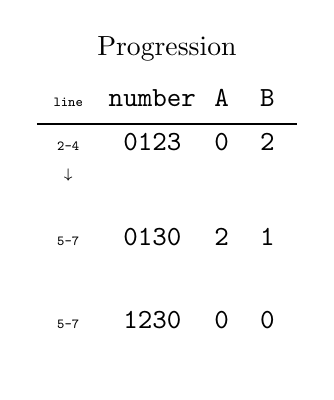
\begin{tikzpicture}[
				value/.style={font=\ttfamily},
				leading/.style={value, inner xsep=8pt, xshift=2pt},
				indicator/.style={inner sep=0, font=\ttfamily\scriptsize},
				line/.style={inner sep=6pt, font=\ttfamily\tiny}]
	
				\node (title) {Progression};
	
				\matrix (progress)  [
					below=0em of title,
					matrix of nodes, 
					column 1/.style={line},
					column 2/.style={value},
					column 3/.style={value},
					column 4/.style={leading}] {
	
					line & number & A & B \\
					\hline
	
					2-4 & 0123 & 0 & 2 \\[-1.3ex]
					$\downarrow$ & ~~~~~ & & \\[0.8em]
	
					5-7 & 0130 & 2 & 1 \\[-1.3ex]
					$\circlearrowright$ & ~~~~~ & & \\[0.8em]
	
					5-7 & 1230 & 0 & 0 \\[-1.3ex]
					$\circlearrowright$ & ~~~~~ & & \\
				};
	
				\ByteIndicator{3};
				\ByteIndicator{5};
				\ByteIndicator{7};
	
				\HLindicator{3}{3.15ex};
				\HLindicator{5}{0.8ex};
				\HLindicator{7}{-1.45ex};
	
			\end{tikzpicture}

		\end{tabular}

		\begin{DetailEffects}[p]
			\FlagsRLD
		\end{DetailEffects}
						
		\begin{DetailTiming}
			\DetailTime{5}{18}
		\end{DetailTiming}

		\DetailNote{Note: instruction doesn't assume any format of the data; it simply rotates nibbles. So while it's most frequently associated with BCD numbers, it can be used for shifting hexadecimal values (in which case it would represent multiplication by {\tt 16}), or any other content.}

	\end{DetailItem}

	\begin{DetailItem}{RR s}
		{\IH{R}otate \IH{R}ight}
		{\SymRR{s}}

		\begin{DetailVariants}
			RR A\\
			RR B\\
			RR C\\
			RR D\\
			RR E\\
			RR H\\
			RR L\\
			RR (HL)\\
			RR (IX+d)\\
			RR (IY+d)

			\columnbreak
			RR (IX+d),A\UNDOC\\
			RR (IX+d),B\UNDOC\\
			RR (IX+d),C\UNDOC\\
			RR (IX+d),D\UNDOC\\
			RR (IX+d),E\UNDOC\\
			RR (IX+d),H\UNDOC\\
			RR (IX+d),L\UNDOC

			\columnbreak
			RR (IY+d),A\UNDOC\\
			RR (IY+d),B\UNDOC\\
			RR (IY+d),C\UNDOC\\
			RR (IY+d),D\UNDOC\\
			RR (IY+d),E\UNDOC\\
			RR (IY+d),H\UNDOC\\
			RR (IY+d),L\UNDOC
		\end{DetailVariants}

		Performs 9-bit right rotation of the contens of the operand {\tt s} or memory addressed by {\tt s} through carry flag {\tt CF} so that contents of {\tt CF} are moved to bit {\tt 7} and bit {\tt 0} to {\tt CF}. Result is then stored back to {\tt s}.

		\begin{DetailEffects}[p]
			\FlagsRRr
		\end{DetailEffects}
						
		\begin{DetailTiming}
			\DetailTime[r]{2}{8}
			\DetailTime[(HL)]{4}{15}
			\DetailTime[(IX+d)]{6}{23}
			\DetailTime[(IY+d)]{6}{23}
		\end{DetailTiming}

	\end{DetailItem}

	\begin{DetailItem}{RRA}
		{\IH{R}otate \IH{R}ight \IH{A}ccumulator}
		{\SymRR{A}}

		Performs {\tt RR A}, but twice faster and preserves {\tt SF} and {\tt ZF}.

		\begin{DetailEffects}
			\FlagsRRA
		\end{DetailEffects}
						
		\begin{DetailTiming}
			\DetailTime{1}{4}
		\end{DetailTiming}

	\end{DetailItem}

	\pagebreak
	\begin{DetailItem}{RRC s}
		{\IH{R}otate \IH{R}ight \IH{C}ircular}
		{\SymRRC{s}}

		\begin{DetailVariants}
			RRC A\\
			RRC B\\
			RRC C\\
			RRC D\\
			RRC E\\
			RRC H\\
			RRC L\\
			RRC (HL)\\
			RRC (IX+d)\\
			RRC (IY+d)

			\columnbreak
			RRC (IX+d),A\UNDOC\\
			RRC (IX+d),B\UNDOC\\
			RRC (IX+d),C\UNDOC\\
			RRC (IX+d),D\UNDOC\\
			RRC (IX+d),E\UNDOC\\
			RRC (IX+d),H\UNDOC\\
			RRC (IX+d),L\UNDOC

			\columnbreak
			RRC (IY+d),A\UNDOC\\
			RRC (IY+d),B\UNDOC\\
			RRC (IY+d),C\UNDOC\\
			RRC (IY+d),D\UNDOC\\
			RRC (IY+d),E\UNDOC\\
			RRC (IY+d),H\UNDOC\\
			RRC (IY+d),L\UNDOC
		\end{DetailVariants}

		Performs 8-bit rotation of the source {\tt s} to the right. Bit {\tt 0} is moved to {\tt CF} as well as to bit {\tt 7}. Result is then stored back to {\tt s}.

		\begin{DetailEffects}[p]
			\FlagsRRCr
		\end{DetailEffects}
						
		\begin{DetailTiming}
			\DetailTime[r]{2}{8}
			\DetailTime[(HL)]{4}{15}
			\DetailTime[(IX+d)]{6}{23}
			\DetailTime[(IY+d)]{6}{23}
		\end{DetailTiming}

	\end{DetailItem}

	\begin{DetailItem}{RRCA}
		{\IH{R}otate \IH{R}ight \IH{C}ircular \IH{A}ccumulator}
		{\SymRRC{A}}

		Performs {\tt RRC A}, but twice faster and preserves {\tt SF} and {\tt ZF}.

		\begin{DetailEffects}
			\FlagsRRCA
		\end{DetailEffects}
						
		\begin{DetailTiming}
			\DetailTime{1}{4}
		\end{DetailTiming}

	\end{DetailItem}

	\begin{DetailItem}{RRD}
		{\IH{R}otate \IH{R}ight bcd \IH{D}igit}
		{\SymRRD}
		
		Similar to {\tt RLD} (page \pageref{DetailRefRLD}) except rotation is to the right. If used with BCD values, this operation effectively divides 3-digit BCD number by {\tt 10} and stores remainder in {\tt A}. Taking example from {\tt RLD}, we can easily convert it to division by 10 simply by using {\tt RRD}. Note however we also need to change the order - we start from MSB now (which is exactly how division would be performed by hand):

		\begin{tabular}{m{8cm}p{0.1cm}m{4.3cm}}

			\begin{lstlisting}[autogobble=true, belowskip=0pt]
			divideBy10:
				LD HL, number	; number=0123
				LD B, digits	; number of repeats
				XOR A			; reset "carry"
			lp:	RRD				; divide by 10 
				INC HL			; next 2 digits
				DJNZ lp			; number=0012, A=3

			number:
				DB $01, $23
			digits: = $ - number ;(2)
			\end{lstlisting}
	
			& &
   	
			\newcommand{\HLindicator}[2]{
				\path (progress-#1-2.south west) --
					node[xshift=#2, yshift=1.4ex, rotate=90]{$\lbrace$}
					node[xshift=#2 + 0.1ex, yshift=0.2ex, indicator]{(HL)} (progress-#1-2.south)
			}

			\newcommand{\ByteIndicator}[1]{
				\draw 
					(progress-#1-2.west) ++(8.5pt,9pt) 
					|- ++(5pt,-3pt) -| ++(6pt,3pt) 
					++(1pt,0) 
					|- ++(5pt,-3pt) -| ++(6pt,3pt);
			}
	
			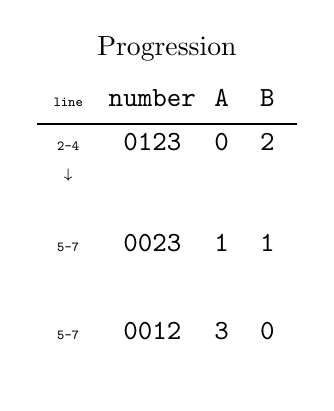
\begin{tikzpicture}[
				value/.style={font=\ttfamily},
				leading/.style={value, inner xsep=8pt, xshift=2pt},
				indicator/.style={inner sep=0, font=\ttfamily\scriptsize},
				line/.style={inner sep=6pt, font=\ttfamily\tiny}]
	
				\node (title) {Progression};
	
				\matrix (progress)  [
					below=0em of title,
					matrix of nodes, 
					column 1/.style={line},
					column 2/.style={value},
					column 3/.style={value},
					column 4/.style={leading}] {

					line & number & A & B \\
					\hline

					2-4 & 0123 & 0 & 2 \\[-1.3ex]
					$\downarrow$ & ~~~~~ & & \\[1em]

					5-7 & 0023 & 1 & 1 \\[-1.3ex]
					$\circlearrowright$ & ~~~~~ & & \\[1em]

					5-7 & 0012 & 3 & 0 \\[-1.3ex]
					$\circlearrowright$ & ~~~~~  & \\[1em]
				};
	
				\ByteIndicator{3};
				\ByteIndicator{5};
				\ByteIndicator{7};
		
				\HLindicator{3}{0.8ex};
				\HLindicator{5}{3.15ex};
				\HLindicator{7}{5.4ex};
	
			\end{tikzpicture}	

		\end{tabular}
		
		\begin{DetailEffects}[p]
			\FlagsRRD
		\end{DetailEffects}
						
		\begin{DetailTiming}
			\DetailTime{5}{18}
		\end{DetailTiming}

	\end{DetailItem}

	\begin{DetailItem}{RST n}
		{\IH{R}e\IH{ST}art}
		{\SymRST{n}}

		\begin{DetailVariants}
			RST \$00\\
			RST \$08\\
			RST \$10\\
			RST \$18
			
			\columnbreak
			RST \$20\\
			RST \$28\\
			RST \$30\\
			RST \$38
		\end{DetailVariants}

		Restarts at the zero page address {\tt s}. Only above addresses are possible, all in page {\tt 0} of the memory, therefore most significant byte of the program counter {\tt PC} is loaded with {\tt \$00}. The instruction may be used as a fast response to an interrupt.

		\begin{DetailEffects}
			\FlagsRSTn				
		\end{DetailEffects}

		\begin{DetailTiming}
			\DetailTime{3}{11}
		\end{DetailTiming}

	\end{DetailItem}

	\pagebreak
	\begin{DetailItem}{SBC d,s}
		{\IH{S}u\IH{B}tract with \IH{C}arry}
		{\SymSBC{d}{s}}
	
		\begin{DetailVariants}
			\textnormal{8 bit}\\
			SBC A,A\\
			SBC A,B\\
			SBC A,C\\
			SBC A,D\\
			SBC A,E\\
			SBC A,H\\
			SBC A,L\\
			SBC A,n

			\columnbreak
			\textnormal{8 bit}\\
			SBC A,IXH\UNDOC\\
			SBC A,IXL\UNDOC\\
			SBC A,IYH\UNDOC\\
			SBC A,IYL\UNDOC\\
			SBC A,(HL)\\
			SBC A,(IX+d)\\
			SBC A,(IY+d)

			\columnbreak
			\textnormal{16 bit}\\
			SBC HL,BC\\
			SBC HL,DE\\
			SBC HL,HL\\
			SBC HL,SP
		\end{DetailVariants}
		
		Subtracts source operand {\tt s} or contents of the memory location addressed by {\tt s} and carry flag {\tt CF} from destination {\tt d}. Result is then stored to destination {\tt d}.

		\begin{DetailEffects}[v]
			\FlagsSBCr[8-bit]
			\FlagsSBCrr[16-bit]
			\DetailFlagsComments{
				\item 16-bit: {\tt HF} set by carry from bit 11 (half carry in high byte)
			}
		\end{DetailEffects}
						
		\begin{DetailTiming}
			\DetailTime[r]{1}{4}
			\DetailTime[n]{2}{7}
			\DetailTime[(HL)]{2}{7}
			\DetailTime[HL,rr]{4}{15}
			\DetailTime[(IX+d)]{5}{19}
			\DetailTime[(IY+d)]{5}{19}
		\end{DetailTiming}

	\end{DetailItem}

	\begin{DetailItem}{SCF}
		{\IH{S}et \IH{C}arry \IH{F}lag}
		{\SymSCF}

		Sets carry flag {\tt CF}.

		\begin{DetailEffects}
			\FlagsSCF
		\end{DetailEffects}
						
		\begin{DetailTiming}
			\DetailTime{1}{4}
		\end{DetailTiming}

	\end{DetailItem}

	\pagebreak
	\begin{DetailItem}{SET b,s}
		{\IH{SET} bit}
		{\SymSET{s}}

		\begin{DetailVariants}
			SET b,A\\
			SET b,B\\
			SET b,C\\
			SET b,D\\
			SET b,E\\
			SET b,H\\
			SET b,L\\
			SET b,(HL)\\
			SET b,(IX+d)\\
			SET b,(IY+d)

			\columnbreak
			SET b,(IX+d),A\UNDOC\\
			SET b,(IX+d),B\UNDOC\\
			SET b,(IX+d),C\UNDOC\\
			SET b,(IX+d),D\UNDOC\\
			SET b,(IX+d),E\UNDOC\\
			SET b,(IX+d),H\UNDOC\\
			SET b,(IX+d),L\UNDOC

			\columnbreak
			SET b,(IY+d),A\UNDOC\\
			SET b,(IY+d),B\UNDOC\\
			SET b,(IY+d),C\UNDOC\\
			SET b,(IY+d),D\UNDOC\\
			SET b,(IY+d),E\UNDOC\\
			SET b,(IY+d),H\UNDOC\\
			SET b,(IY+d),L\UNDOC
		\end{DetailVariants}

		Sets bit {\tt b} ({\tt 0-7}) of operand {\tt s} or memory location addressed by {\tt s}.

		Note: undocumented variants work slightly differently:

		\begin{multicols}{2}
			\DetailSymbolVariants{SET b,(IX+d),r}{\SymSETu{r}{IX}}

			\DetailSymbolVariants{SET b,(IY+d),r}{\SymSETu{r}{IY}}
		\end{multicols}

		\begin{DetailEffects}
			\FlagsSETr
		\end{DetailEffects}			

		\begin{DetailTiming}
			\DetailTime[r]{2}{8}
			\DetailTime[(HL)]{4}{15}
			\DetailTime[(IX+d)]{6}{23}
			\DetailTime[(IY+d)]{6}{23}
		\end{DetailTiming}

	\end{DetailItem}

	\begin{DetailItem}{SETAE\ZXN}
		{\IH{SET} \IH{A}ccumulator from \IH{E}}
		{\SymSETAE}

		Takes the bit number to set from {\tt E} (only the low 3 bits) and sets the value of the accumulator {\tt A} to the value of that bit, but counted from top to bottom ({\tt E=0} will produce {\tt A$\leftarrow$\$80}, {\tt E=7} will produce {\tt A$\leftarrow$\$01} and so on). This works as pixel mask for ULA bitmap modes, when {\tt E} represents x-coordinate {\tt 0-255}.

		\begin{DetailEffects}
			\FlagsSETAE
		\end{DetailEffects}
						
		\begin{DetailTiming}
			\DetailTime{2}{8}
		\end{DetailTiming}

	\end{DetailItem}

	\pagebreak
	\begin{DetailItem}{SLA s}
		{\IH{S}hift \IH{L}eft \IH{A}rithmetic}
		{\SymSLA{s}}
		
		\begin{DetailVariants}
			SLA A\\
			SLA B\\
			SLA C\\
			SLA D\\
			SLA E\\
			SLA H\\
			SLA L\\
			SLA (HL)\\
			SLA (IX+d)\\
			SLA (IY+d)

			\columnbreak
			SLA (IX+d),A\UNDOC\\
			SLA (IX+d),B\UNDOC\\
			SLA (IX+d),C\UNDOC\\
			SLA (IX+d),D\UNDOC\\
			SLA (IX+d),E\UNDOC\\
			SLA (IX+d),H\UNDOC\\
			SLA (IX+d),L\UNDOC

			\columnbreak
			SLA (IY+d),A\UNDOC\\
			SLA (IY+d),B\UNDOC\\
			SLA (IY+d),C\UNDOC\\
			SLA (IY+d),D\UNDOC\\
			SLA (IY+d),E\UNDOC\\
			SLA (IY+d),H\UNDOC\\
			SLA (IY+d),L\UNDOC
		\end{DetailVariants}

		Performs arithmetic shift left of the operand {\tt s} or memory location addressed by {\tt s}. Bit {\tt 0} is forced to {\tt 0} and bit {\tt 7} is moved to {\tt CF}.

		\begin{DetailEffects}[p]
			\FlagsSLAr
		\end{DetailEffects}
						
		\begin{DetailTiming}
			\DetailTime[r]{2}{8}
			\DetailTime[(HL)]{4}{15}
			\DetailTime[(IX+d)]{6}{23}
			\DetailTime[(IY+d)]{6}{23}
		\end{DetailTiming}

	\end{DetailItem}

	\begin{DetailItem}{SLL}
		{\IH{S}hift \IH{L}eft \IH{L}ogical}
		{}

		This mnemonic has no associated opcode on Next. There is no difference between logical and arithmetic shift left, use {\tt SLA} for both. Some assemblers will allow {\tt SLL} as equivalent, but unfortunately some will assemble it as {\tt SLI}, so it's best avoiding.
		
	\end{DetailItem}

	\pagebreak
	\begin{DetailItem}{SLI s\UNDOC\\SL1 s\UNDOC}
		{\IH{S}hift \IH{L}eft and \IH{I}ncrement\\
		\IH{S}hift \IH{L}eft and add \IH{1}}
		{\SymSLI{s}}
		
		\begin{DetailVariants}
			SLI A\\
			SLI B\\
			SLI C\\
			SLI D\\
			SLI E\\
			SLI H\\
			SLI L\\
			SLA (HL)\\
			SLA (IX+d)\\
			SLA (IY+d)

			\columnbreak
			SLI (IX+d),A\UNDOC\\
			SLI (IX+d),B\UNDOC\\
			SLI (IX+d),C\UNDOC\\
			SLI (IX+d),D\UNDOC\\
			SLI (IX+d),E\UNDOC\\
			SLI (IX+d),H\UNDOC\\
			SLI (IX+d),L\UNDOC

			\columnbreak
			SLI (IY+d),A\UNDOC\\
			SLI (IY+d),B\UNDOC\\
			SLI (IY+d),C\UNDOC\\
			SLI (IY+d),D\UNDOC\\
			SLI (IY+d),E\UNDOC\\
			SLI (IY+d),H\UNDOC\\
			SLI (IY+d),L\UNDOC
		\end{DetailVariants}

		Undocumented instruction. Similar to {\tt SLA} except {\tt 1} is moved to bit {\tt 0}.

		\begin{DetailEffects}[p]
			\FlagsSLIr
		\end{DetailEffects}
						
		\begin{DetailTiming}
			\DetailTime[r]{2}{8}
			\DetailTime[(HL)]{4}{15}
			\DetailTime[(IX+d)]{6}{23}
			\DetailTime[(IY+d)]{6}{23}
		\end{DetailTiming}

		\DetailNote{Note: most assemblers will accept both variants: {\tt SLI} or {\tt SL1}, but some may only accept one or the other, while some may expect {\tt SLL} instead.}

	\end{DetailItem}

	\pagebreak
	\begin{DetailItem}{SRA s}
		{\IH{S}hift \IH{R}ight \IH{A}rithmetic}
		{\SymSRA{s}}
				
		% we're using non-standard layout here so that we can fit SRA and SRL to the same page
		\begin{DetailVariants}[p{1.3cm}p{3.5cm}XX]
			SRA A	& SRA (HL)		& SRA (IX+d),A\UNDOC	& SRA (IY+d),A\UNDOC \\
			SRA B	& SRA (IX+d)	& SRA (IX+d),B\UNDOC	& SRA (IY+d),B\UNDOC \\
			SRA C	& SRA (IY+d)	& SRA (IX+d),C\UNDOC	& SRA (IY+d),C\UNDOC \\
			SRA D	&				& SRA (IX+d),D\UNDOC	& SRA (IY+d),D\UNDOC \\
			SRA E	&				& SRA (IX+d),E\UNDOC	& SRA (IY+d),E\UNDOC \\
			SRA H	&				& SRA (IX+d),H\UNDOC	& SRA (IY+d),H\UNDOC \\
			SRA L	&				& SRA (IX+d),L\UNDOC	& SRA (IY+d),L\UNDOC \\
		\end{DetailVariants}

		Performs arithmetic shift right of the operand {\tt s} or memory location addressed by {\tt s}. Bit {\tt 0} is moved to {\tt CF} while bit {\tt 7} remains unchanged (on the assumption that it's the sign bit).

		\begin{DetailEffects}[p]
			\FlagsSRAr
		\end{DetailEffects}
						
		\begin{DetailTiming}
			\DetailTime[r]{2}{8}
			\DetailTime[(HL)]{4}{15}
			\DetailTime[(IX+d)]{6}{23}
			\DetailTime[(IY+d)]{6}{23}
		\end{DetailTiming}

	\end{DetailItem}

	\begin{DetailItem}{SRL s}
		{\IH{S}hift \IH{R}ight \IH{L}ogical}
		{\SymSRL{s}}
				
		% we're using non-standard layout here so that we can fit SRA and SRL to the same page
		\begin{DetailVariants}[p{1.3cm}p{3.5cm}XX]
			SRL A	& SRL (HL)		& SRL (IX+d),A\UNDOC	& SRL (IY+d),A\UNDOC \\
			SRL B	& SRL (IX+d)	& SRL (IX+d),B\UNDOC	& SRL (IY+d),B\UNDOC \\
			SRL C	& SRL (IY+d)	& SRL (IX+d),C\UNDOC	& SRL (IY+d),C\UNDOC \\
			SRL D	&				& SRL (IX+d),D\UNDOC	& SRL (IY+d),D\UNDOC \\
			SRL E	&				& SRL (IX+d),E\UNDOC	& SRL (IY+d),E\UNDOC \\
			SRL H	&				& SRL (IX+d),H\UNDOC	& SRL (IY+d),H\UNDOC \\
			SRL L	&				& SRL (IX+d),L\UNDOC	& SRL (IY+d),L\UNDOC \\
		\end{DetailVariants}

		Performs logical shift right of the operand {\tt s} or memory location addressed by {\tt s}. Bit {\tt 0} is moved to {\tt CF} while {\tt 0} is moved to bit {\tt 7}.

		\begin{DetailEffects}[p]
			\FlagsSRLr
		\end{DetailEffects}
						
		\begin{DetailTiming}
			\DetailTime[r]{2}{8}
			\DetailTime[(HL)]{4}{15}
			\DetailTime[(IX+d)]{6}{23}
			\DetailTime[(IY+d)]{6}{23}
		\end{DetailTiming}

	\end{DetailItem}

	\pagebreak
	\begin{DetailItem}{SUB s}
		{\IH{SUB}tract}
		{\SymSUB{s}}

		\begin{DetailVariants}
			SUB A\\
			SUB B\\
			SUB C\\
			SUB D\\
			SUB E\\
			SUB H\\
			SUB L

			\columnbreak
			SUB n\\
			SUB (HL)\\
			SUB (IX+d)\\
			SUB (IY+d)

			\columnbreak
			SUB IXH\UNDOC\\
			SUB IXL\UNDOC\\
			SUB IYH\UNDOC\\
			SUB IYL\UNDOC
		\end{DetailVariants}

		Subtracts 8-bit immediate value, operand {\tt s} or memory location addressed by {\tt c} from accumulator {\tt A}. Then stores result back to {\tt A}.

		\begin{DetailEffects}[v]
			\FlagsSUBr
		\end{DetailEffects}
						
		\begin{DetailTiming}
			\DetailTime[r]{1}{4}
			\DetailTime[n]{2}{7}
			\DetailTime[(HL)]{2}{7}
			\DetailTime[(IX+d)]{5}{19}
			\DetailTime[(IY+d)]{5}{19}
		\end{DetailTiming}

	\end{DetailItem}

	\begin{DetailItem}{SWAPNIB\ZXN}
		{\IH{SWAP} \IH{NIB}bles}
		{\SymSWAPNIB}

		Swaps the high and low nibbles of accumulator {\tt A}.

		\begin{DetailEffects}
			\FlagsSWAPNIB
		\end{DetailEffects}
						
		\begin{DetailTiming}
			\DetailTime{2}{8}
		\end{DetailTiming}

	\end{DetailItem}

	\begin{DetailItem}{TEST n\ZXN}
		{\IH{TEST}}
		{\SymTEST}

		Similar to {\tt CP} (page \pageref{DetailRefCP}), but performs an {\tt AND} instead of a subtraction.

		\begin{DetailEffects}[v]
			\FlagsTESTn
		\end{DetailEffects}
						
		\begin{DetailTiming}
			\DetailTime{3}{11}
		\end{DetailTiming}

	\end{DetailItem}

	\pagebreak
	\begin{DetailItem}{XOR s}
		{bitwise e\IH{X}clusive \IH{OR}}
		{\SymXOR{s}}

		\begin{DetailVariants}
			XOR A\\
			XOR B\\
			XOR C\\
			XOR D\\
			XOR E\\
			XOR H\\
			XOR L\\
			XOR n

			\columnbreak
			XOR (HL)\\
			XOR (IX+d)\\
			XOR (IY+d)

			\columnbreak
			XOR IXH\UNDOC\\
			XOR IXL\UNDOC\\
			XOR IYH\UNDOC\\
			XOR IYL\UNDOC
		\end{DetailVariants}

		Performs exclusive or between accumulator {\tt A} and operand {\tt s} or memory location addressed by {\tt s}. Result is then stored back to {\tt A}. Individual bits are XOR'ed like this:

		\begin{tabular}{cc|c}
			{\tt A} & {\tt s} & Result \\
			\hline
			{\tt 0} & {\tt 0} & {\tt 0} \\
			{\tt 0} & {\tt 1} & {\tt 1} \\
			{\tt 1} & {\tt 0} & {\tt 1} \\
			{\tt 1} & {\tt 1} & {\tt 0} \\
		\end{tabular}

		\begin{DetailEffects}[p]
			\FlagsXORr
		\end{DetailEffects}
						
		\begin{DetailTiming}
			\DetailTime[r]{1}{4}
			\DetailTime[n]{2}{7}
			\DetailTime[(HL)]{2}{7}
			\DetailTime[(IX+d)]{5}{19}
			\DetailTime[(IY+d)]{5}{19}
		\end{DetailTiming}

	\end{DetailItem}

\end{basedescript}


\pagebreak
\IntentionallyEmpty
\pagebreak


\appendix

% only print chapters in appendices, not sections and subsections
\addtocontents{toc}{\protect\setcounter{tocdepth}{0}}


\chapter{Instructions Sorted by Mnemonic}

% █████████████████████████████████████████████████████████████████████████████████████
% █░░░░░░██████████░░░░░░█░░░░░░██████████░░░░░░█░░░░░░░░░░░░░░█░░░░░░██████████░░░░░░█
% █░░▄▀░░░░░░░░░░░░░░▄▀░░█░░▄▀░░░░░░░░░░██░░▄▀░░█░░▄▀▄▀▄▀▄▀▄▀░░█░░▄▀░░░░░░░░░░░░░░▄▀░░█
% █░░▄▀▄▀▄▀▄▀▄▀▄▀▄▀▄▀▄▀░░█░░▄▀▄▀▄▀▄▀▄▀░░██░░▄▀░░█░░▄▀░░░░░░░░░░█░░▄▀▄▀▄▀▄▀▄▀▄▀▄▀▄▀▄▀░░█
% █░░▄▀░░░░░░▄▀░░░░░░▄▀░░█░░▄▀░░░░░░▄▀░░██░░▄▀░░█░░▄▀░░█████████░░▄▀░░░░░░▄▀░░░░░░▄▀░░█
% █░░▄▀░░██░░▄▀░░██░░▄▀░░█░░▄▀░░██░░▄▀░░██░░▄▀░░█░░▄▀░░░░░░░░░░█░░▄▀░░██░░▄▀░░██░░▄▀░░█
% █░░▄▀░░██░░▄▀░░██░░▄▀░░█░░▄▀░░██░░▄▀░░██░░▄▀░░█░░▄▀▄▀▄▀▄▀▄▀░░█░░▄▀░░██░░▄▀░░██░░▄▀░░█
% █░░▄▀░░██░░░░░░██░░▄▀░░█░░▄▀░░██░░▄▀░░██░░▄▀░░█░░▄▀░░░░░░░░░░█░░▄▀░░██░░░░░░██░░▄▀░░█
% █░░▄▀░░██████████░░▄▀░░█░░▄▀░░██░░▄▀░░░░░░▄▀░░█░░▄▀░░█████████░░▄▀░░██████████░░▄▀░░█
% █░░▄▀░░██████████░░▄▀░░█░░▄▀░░██░░▄▀▄▀▄▀▄▀▄▀░░█░░▄▀░░░░░░░░░░█░░▄▀░░██████████░░▄▀░░█
% █░░▄▀░░██████████░░▄▀░░█░░▄▀░░██░░░░░░░░░░▄▀░░█░░▄▀▄▀▄▀▄▀▄▀░░█░░▄▀░░██████████░░▄▀░░█
% █░░░░░░██████████░░░░░░█░░░░░░██████████░░░░░░█░░░░░░░░░░░░░░█░░░░░░██████████░░░░░░█
% █████████████████████████████████████████████████████████████████████████████████████

Instructions marked with \UNDOC ~are undocumented.\\
Instructions marked with \ZXN ~are ZX Spectrum Next extended.
% TODO: and any instruction not listed has no effect? (same behaviour as an equal amount of NOP instructions)
\setlength\columnsep{4em}
\begin{multicols}{3}
{
	\tt 
	\footnotesize
	\begin{tabbing}
		ADC A,A~~~~{\qquad}{\quad}\=8F\\
		ADC A,B\>88\\
		ADC A,C\>89\\
		ADC A,D\>8A\\
		ADC A,E\>8B\\
		ADC A,H\>8C\\
		ADC A,L\>8D\\
		ADC A,n\>CE n\\
		ADC A,(HL)\>8E\\
		ADC A,(IX+d)\>DD8E d\\
		ADC A,(IY+d)\>FD8E d\\
		ADC A,IXH\UNDOC\>DD8C\\
		ADC A,IXL\UNDOC\>DD8D\\
		ADC A,IYH\UNDOC\>FD8C\\
		ADC A,IYL\UNDOC\>FD8D\\
		ADC HL,BC\>ED4A\\
		ADC HL,DE\>ED5A\\
		ADC HL,HL\>ED6A\\
		ADC HL,SP\>ED7A\\
		ADD A,A\>87\\
		ADD A,B\>80\\
		ADD A,C\>81\\
		ADD A,D\>82\\
		ADD A,E\>83\\
		ADD A,H\>84\\
		ADD A,L\>85\\
		ADD A,n\>C6 n\\
		ADD A,(HL)\>86\\
		ADD A,(IX+d)\>DD86 d\\
		ADD A,(IY+d)\>FD86 d\\
		ADD A,IXH\UNDOC\>DD84\\
		ADD A,IXL\UNDOC\>DD85\\
		ADD A,IYH\UNDOC\>FD84\\
		ADD A,IYL\UNDOC\>FD85\\
		ADD BC,A\ZXN\>ED33\\
		ADD BC,nm\ZXN\>ED36	m n\\
		ADD DE,A\ZXN\>ED32\\
		ADD DE,nm\ZXN\>ED35 m n\\
		ADD HL,A\ZXN\>ED31\\
		ADD HL,BC\>09\\
		ADD HL,DE\>19\\
		ADD HL,HL\>29\\
		ADD HL,SP\>39\\
		ADD HL,nm\ZXN\>ED34 m n\\
		ADD IX,BC\>DD09\\
		ADD IX,DE\>DD19\\
		ADD IX,IX\>DD29\\
		ADD IX,SP\>DD39\\
		ADD IY,BC\>FD09\\
		ADD IY,DE\>FD19\\
		ADD IY,IY\>FD29\\
		ADD IY,SP\>FD39\\
		AND A\>A7\\
		AND B\>A0\\
		AND C\>A1\\
		AND D\>A2\\
		AND E\>A3\\
		AND H\>A4\\
		AND L\>A5\\
		AND n\>E6 n\\
		AND (HL)\>A6\\
		AND (IX+d)\>DDA6 d\\
		AND (IY+d)\>FDA6 d\\
		AND IXH\UNDOC\>DDA4\\
		AND IXL\UNDOC\>DDA5\\
		AND IYH\UNDOC\>FDA4\\
		AND IYL\UNDOC\>FDA5\\
		BIT 0,A\>CB47\\
		BIT 0,B\>CB40\\
		BIT 0,C\>CB41\\
		BIT 0,D\>CB42\\
		BIT 0,E\>CB43\\
		BIT 0,H\>CB44\\
		BIT 0,L\>CB45\\
		BIT 0,(HL)\>CB46\\
		BIT 0,(IX+d)\>DDCB d 46\\
		BIT 0,(IX+d)\UNDOC\>DDCB d 40\\
		BIT 0,(IX+d)\UNDOC\>DDCB d 41\\
		BIT 0,(IX+d)\UNDOC\>DDCB d 42\\
		BIT 0,(IX+d)\UNDOC\>DDCB d 43\\
		BIT 0,(IX+d)\UNDOC\>DDCB d 44\\
		BIT 0,(IX+d)\UNDOC\>DDCB d 45\\
		BIT 0,(IX+d)\UNDOC\>DDCB d 47\\
		BIT 0,(IY+d)\>FDCB d 46\\
		BIT 0,(IY+d)\UNDOC\>FDCB d 40\\
		BIT 0,(IY+d)\UNDOC\>FDCB d 41\\
		BIT 0,(IY+d)\UNDOC\>FDCB d 42\\
		BIT 0,(IY+d)\UNDOC\>FDCB d 43\\
		BIT 0,(IY+d)\UNDOC\>FDCB d 44\\
		BIT 0,(IY+d)\UNDOC\>FDCB d 45\\
		BIT 0,(IY+d)\UNDOC\>FDCB d 47\\
		BIT 1,A\>CB4F\\
		BIT 1,B\>CB48\\
		BIT 1,C\>CB49\\
		BIT 1,D\>CB4A\\
		BIT 1,E\>CB4B\\
		BIT 1,H\>CB4C\\
		BIT 1,L\>CB4D\\
		BIT 1,(HL)\>CB4E\\
		BIT 1,(IX+d)\>DDCB d 4E\\
		BIT 1,(IX+d)\UNDOC\>DDCB d 48\\
		BIT 1,(IX+d)\UNDOC\>DDCB d 49\\
		BIT 1,(IX+d)\UNDOC\>DDCB d 4A\\
		BIT 1,(IX+d)\UNDOC\>DDCB d 4B\\
		BIT 1,(IX+d)\UNDOC\>DDCB d 4C\\
		BIT 1,(IX+d)\UNDOC\>DDCB d 4D\\
		BIT 1,(IX+d)\UNDOC\>DDCB d 4F\\
		BIT 1,(IY+d)\>FDCB d 4E\\
		BIT 1,(IY+d)\UNDOC\>FDCB d 48\\
		BIT 1,(IY+d)\UNDOC\>FDCB d 49\\
		BIT 1,(IY+d)\UNDOC\>FDCB d 4A\\
		BIT 1,(IY+d)\UNDOC\>FDCB d 4B\\
		BIT 1,(IY+d)\UNDOC\>FDCB d 4C\\
		BIT 1,(IY+d)\UNDOC\>FDCB d 4D\\
		BIT 1,(IY+d)\UNDOC\>FDCB d 4F\\
		BIT 2,A\>CB57\\
		BIT 2,B\>CB50\\
		BIT 2,C\>CB51\\
		BIT 2,D\>CB52\\
		BIT 2,E\>CB53\\
		BIT 2,H\>CB54\\
		BIT 2,L\>CB55\\
		BIT 2,(HL)\>CB56\\
		BIT 2,(IX+d)\>DDCB d 56\\
		BIT 2,(IX+d)\UNDOC\>DDCB d 50\\
		BIT 2,(IX+d)\UNDOC\>DDCB d 51\\
		BIT 2,(IX+d)\UNDOC\>DDCB d 52\\
		BIT 2,(IX+d)\UNDOC\>DDCB d 53\\
		BIT 2,(IX+d)\UNDOC\>DDCB d 54\\
		BIT 2,(IX+d)\UNDOC\>DDCB d 55\\
		BIT 2,(IX+d)\UNDOC\>DDCB d 57\\
		BIT 2,(IY+d)\>FDCB d 56\\
		BIT 2,(IY+d)\UNDOC\>FDCB d 50\\
		BIT 2,(IY+d)\UNDOC\>FDCB d 51\\
		BIT 2,(IY+d)\UNDOC\>FDCB d 52\\
		BIT 2,(IY+d)\UNDOC\>FDCB d 53\\
		BIT 2,(IY+d)\UNDOC\>FDCB d 54\\
		BIT 2,(IY+d)\UNDOC\>FDCB d 55\\
		BIT 2,(IY+d)\UNDOC\>FDCB d 57\\
		BIT 3,A\>CB5F\\
		BIT 3,B\>CB58\\
		BIT 3,C\>CB59\\
		BIT 3,D\>CB5A\\
		BIT 3,E\>CB5B\\
		BIT 3,H\>CB5C\\
		BIT 3,L\>CB5D\\
		BIT 3,(HL)\>CB5E\\
		BIT 3,(IX+d)\>DDCB d 5E\\
		BIT 3,(IX+d)\UNDOC\>DDCB d 58\\
		BIT 3,(IX+d)\UNDOC\>DDCB d 59\\
		BIT 3,(IX+d)\UNDOC\>DDCB d 5A\\
		BIT 3,(IX+d)\UNDOC\>DDCB d 5B\\
		BIT 3,(IX+d)\UNDOC\>DDCB d 5C\\
		BIT 3,(IX+d)\UNDOC\>DDCB d 5D\\
		BIT 3,(IX+d)\UNDOC\>DDCB d 5F\\
		BIT 3,(IY+d)\>FDCB d 5E\\
		BIT 3,(IY+d)\UNDOC\>FDCB d 58\\
		BIT 3,(IY+d)\UNDOC\>FDCB d 59\\
		BIT 3,(IY+d)\UNDOC\>FDCB d 5A\\
		BIT 3,(IY+d)\UNDOC\>FDCB d 5B\\
		BIT 3,(IY+d)\UNDOC\>FDCB d 5C\\
		BIT 3,(IY+d)\UNDOC\>FDCB d 5D\\
		BIT 3,(IY+d)\UNDOC\>FDCB d 5F\\
		BIT 4,A\>CB67\\
		BIT 4,B\>CB60\\
		BIT 4,C\>CB61\\
		BIT 4,D\>CB62\\
		BIT 4,E\>CB63\\
		BIT 4,H\>CB64\\
		BIT 4,L\>CB65\\
		BIT 4,(HL)\>CB66\\
		BIT 4,(IX+d)\>DDCB d 66\\
		BIT 4,(IX+d)\UNDOC\>DDCB d 60\\
		BIT 4,(IX+d)\UNDOC\>DDCB d 61\\
		BIT 4,(IX+d)\UNDOC\>DDCB d 62\\
		BIT 4,(IX+d)\UNDOC\>DDCB d 63\\
		BIT 4,(IX+d)\UNDOC\>DDCB d 64\\
		BIT 4,(IX+d)\UNDOC\>DDCB d 65\\
		BIT 4,(IX+d)\UNDOC\>DDCB d 67\\
		BIT 4,(IY+d)\>FDCB d 66\\
		BIT 4,(IY+d)\UNDOC\>FDCB d 60\\
		BIT 4,(IY+d)\UNDOC\>FDCB d 61\\
		BIT 4,(IY+d)\UNDOC\>FDCB d 62\\
		BIT 4,(IY+d)\UNDOC\>FDCB d 63\\
		BIT 4,(IY+d)\UNDOC\>FDCB d 64\\
		BIT 4,(IY+d)\UNDOC\>FDCB d 65\\
		BIT 4,(IY+d)\UNDOC\>FDCB d 67\\
		BIT 5,A\>CB6F\\
		BIT 5,B\>CB68\\
		BIT 5,C\>CB69\\
		BIT 5,D\>CB6A\\
		BIT 5,E\>CB6B\\
		BIT 5,H\>CB6C\\
		BIT 5,L\>CB6D\\
		BIT 5,(HL)\>CB6E\\
		BIT 5,(IX+d)\>DDCB d 6E\\
		BIT 5,(IX+d)\UNDOC\>DDCB d 68\\
		BIT 5,(IX+d)\UNDOC\>DDCB d 69\\
		BIT 5,(IX+d)\UNDOC\>DDCB d 6A\\
		BIT 5,(IX+d)\UNDOC\>DDCB d 6B\\
		BIT 5,(IX+d)\UNDOC\>DDCB d 6C\\
		BIT 5,(IX+d)\UNDOC\>DDCB d 6D\\
		BIT 5,(IX+d)\UNDOC\>DDCB d 6F\\
		BIT 5,(IY+d)\>FDCB d 6E\\
		BIT 5,(IY+d)\UNDOC\>FDCB d 68\\
		BIT 5,(IY+d)\UNDOC\>FDCB d 69\\
		BIT 5,(IY+d)\UNDOC\>FDCB d 6A\\
		BIT 5,(IY+d)\UNDOC\>FDCB d 6B\\
		BIT 5,(IY+d)\UNDOC\>FDCB d 6C\\
		BIT 5,(IY+d)\UNDOC\>FDCB d 6D\\
		BIT 5,(IY+d)\UNDOC\>FDCB d 6F\\
		BIT 6,A\>CB77\\
		BIT 6,B\>CB70\\
		BIT 6,C\>CB71\\
		BIT 6,D\>CB72\\
		BIT 6,E\>CB73\\
		BIT 6,H\>CB74\\
		BIT 6,L\>CB75\\
		BIT 6,(HL)\>CB76\\
		BIT 6,(IX+d)\>DDCB d 76\\
		BIT 6,(IX+d)\UNDOC\>DDCB d 70\\
		BIT 6,(IX+d)\UNDOC\>DDCB d 71\\
		BIT 6,(IX+d)\UNDOC\>DDCB d 72\\
		BIT 6,(IX+d)\UNDOC\>DDCB d 73\\
		BIT 6,(IX+d)\UNDOC\>DDCB d 74\\
		BIT 6,(IX+d)\UNDOC\>DDCB d 75\\
		BIT 6,(IX+d)\UNDOC\>DDCB d 77\\
		BIT 6,(IY+d)\>FDCB d 76\\
		BIT 6,(IY+d)\UNDOC\>FDCB d 70\\
		BIT 6,(IY+d)\UNDOC\>FDCB d 71\\
		BIT 6,(IY+d)\UNDOC\>FDCB d 72\\
		BIT 6,(IY+d)\UNDOC\>FDCB d 73\\
		BIT 6,(IY+d)\UNDOC\>FDCB d 74\\
		BIT 6,(IY+d)\UNDOC\>FDCB d 75\\
		BIT 6,(IY+d)\UNDOC\>FDCB d 77\\
		BIT 7,A\>CB7F\\
		BIT 7,B\>CB78\\
		BIT 7,C\>CB79\\
		BIT 7,D\>CB7A\\
		BIT 7,E\>CB7B\\
		BIT 7,H\>CB7C\\
		BIT 7,L\>CB7D\\
		BIT 7,(HL)\>CB7E\\
		BIT 7,(IX+d)\>DDCB d 7E\\
		BIT 7,(IX+d)\UNDOC\>DDCB d 78\\
		BIT 7,(IX+d)\UNDOC\>DDCB d 79\\
		BIT 7,(IX+d)\UNDOC\>DDCB d 7A\\
		BIT 7,(IX+d)\UNDOC\>DDCB d 7B\\
		BIT 7,(IX+d)\UNDOC\>DDCB d 7C\\
		BIT 7,(IX+d)\UNDOC\>DDCB d 7D\\
		BIT 7,(IX+d)\UNDOC\>DDCB d 7F\\
		BIT 7,(IY+d)\>FDCB d 7E\\
		BIT 7,(IY+d)\UNDOC\>FDCB d 78\\
		BIT 7,(IY+d)\UNDOC\>FDCB d 79\\
		BIT 7,(IY+d)\UNDOC\>FDCB d 7A\\
		BIT 7,(IY+d)\UNDOC\>FDCB d 7B\\
		BIT 7,(IY+d)\UNDOC\>FDCB d 7C\\
		BIT 7,(IY+d)\UNDOC\>FDCB d 7D\\
		BIT 7,(IY+d)\UNDOC\>FDCB d 7F\\
		BRLC DE,B\ZXN\>ED2C\\
		BSLA DE,B\ZXN\>ED28\\
		BSRA DE,B\ZXN\>ED29\\
		BSRF DE,B\ZXN\>ED2B\\
		BSRL DE,B\ZXN\>ED2A\\
		CALL nm\>CD m n\\
		CALL C,nm\>DC m n\\
		CALL M,nm\>FC m n\\
		CALL NC,nm\>D4 m n\\
		CALL NZ,nm\>C4 m n\\
		CALL P,nm\>F4 m n\\
		CALL PE,nm\>EC m n\\
		CALL PO,nm\>E4 m n\\
		CALL Z,nm\>CC m n\\
		CCF\>3F\\
		CP A\>BF\\
		CP B\>B8\\
		CP C\>B9\\
		CP D\>BA\\
		CP E\>BB\\
		CP H\>BC\\
		CP L\>BD\\
		CP n\>FE n\\
		CP (HL)\>BE\\
		CP (IX+d)\>DDBE d\\
		CP (IY+d)\>FDBE d\\
		CP IXH\UNDOC\>DDBC\\
		CP IXL\UNDOC\>DDBD\\
		CP IYH\UNDOC\>FDBC\\
		CP IYL\UNDOC\>FDBD\\
		CPDR\>EDB9\\
		CPD\>EDA9\\
		CPIR\>EDB1\\
		CPI\>EDA1\\
		CPL\>2F\\
		DAA\>27\\
		DEC (HL)\>35\\
		DEC (IX+d)\>DD35 d\\
		DEC (IY+d)\>FD35 d\\
		DEC A\>3D\\
		DEC B\>05\\
		DEC C\>0D\\
		DEC D\>15\\
		DEC E\>1D\\
		DEC H\>25\\
		DEC L\>2D\\
		DEC BC\>0B\\
		DEC DE\>1B\\
		DEC HL\>2B\\
		DEC IX\>DD2B\\
		DEC IXH\UNDOC\>DD25\\
		DEC IXL\UNDOC\>DD2D\\
		DEC IY\>FD2B\\
		DEC IYH\UNDOC\>FD25\\
		DEC IYL\UNDOC\>FD2D\\
		DEC SP\>3B\\
		DI\>F3\\
		DJNZ (PC+e)\>10 e\\
		EI\>FB\\
		EX (SP),HL\>E3\\
		EX (SP),IX\>DDE3\\
		EX (SP),IY\>FDE3\\
		EX AF,AF'\>08\\
		EX DE,HL\>EB\\
		EXX\>D9\\
		HALT\>76\\
		IM 0\UNDOC\>ED4E\\
		IM 0\UNDOC\>ED66\\
		IM 0\UNDOC\>ED6E\\
		IM 0\>ED46\\
		IM 1\UNDOC\>ED76\\
		IM 1\>ED56\\
		IM 2\UNDOC\>ED7E\\
		IM 2\>ED5E\\
		IN A,(C)\>ED78\\
		IN A,(n)\>DB n\\
		IN B,(C)\>ED40\\
		IN C,(C)\>ED48\\
		IN D,(C)\>ED50\\
		IN E,(C)\>ED58\\
		IN F,(C)\UNDOC\>ED70\\
		IN H,(C)\>ED60\\
		IN L,(C)\>ED68\\
		IN (C)\UNDOC\>ED70\\
		INC (HL)\>34\\
		INC (IX+d)\>DD34 d\\
		INC (IY+d)\>FD34 d\\
		INC A\>3C\\
		INC B\>04\\
		INC C\>0C\\
		INC D\>14\\
		INC E\>1C\\
		INC H\>24\\
		INC L\>2C\\
		INC BC\>03\\
		INC DE\>13\\
		INC HL\>23\\
		INC IX\>DD23\\
		INC IXH\UNDOC\>DD24\\
		INC IXL\UNDOC\>DD2C\\
		INC IY\>FD23\\
		INC IYH\UNDOC\>FD24\\
		INC IYL\UNDOC\>FD2C\\
		INC SP\>33\\
		INDR\>EDBA\\
		IND\>EDAA\\
		INIR\>EDB2\\
		INI\>EDA2\\
		JP (C)\ZXN\>ED98\\
		JP (HL)\>E9\\
		JP (IX)\>DDE9\\
		JP (IY)\>FDE9\\
		JP nm\>C3 m n\\
		JP C,nm\>DA m n\\
		JP M,nm\>FA m n\\
		JP NC,nm\>D2 m n\\
		JP NZ,nm\>C2 m n\\
		JP P,nm\>F2 m n\\
		JP PE,nm\>EA m n\\
		JP PO,nm\>E2 m n\\
		JP Z,nm\>CA m n\\
		JR e\>18 e\\
		JR C,e\>38 e\\
		JR NC,e\>30 e\\
		JR NZ,e\>20 e\\
		JR Z,e\>28 e\\
		LD (BC),A\>02\\
		LD (DE),A\>12\\
		LD (HL),A\>77\\
		LD (HL),B\>70\\
		LD (HL),C\>71\\
		LD (HL),D\>72\\
		LD (HL),E\>73\\
		LD (HL),H\>74\\
		LD (HL),L\>75\\
		LD (HL),n\>36 n\\
		LD (IX+d),A\>DD77 d\\
		LD (IX+d),B\>DD70 d\\
		LD (IX+d),C\>DD71 d\\
		LD (IX+d),D\>DD72 d\\
		LD (IX+d),E\>DD73 d\\
		LD (IX+d),H\>DD74 d\\
		LD (IX+d),L\>DD75 d\\
		LD (IX+d),n\>DD36 d n\\
		LD (IY+d),A\>FD77 d\\
		LD (IY+d),B\>FD70 d\\
		LD (IY+d),C\>FD71 d\\
		LD (IY+d),D\>FD72 d\\
		LD (IY+d),E\>FD73 d\\
		LD (IY+d),H\>FD74 d\\
		LD (IY+d),L\>FD75 d\\
		LD (IY+d),n\>FD36 d n\\
		LD (nm),A\>32 m n\\
		LD (nm),BC\>ED43 m n\\
		LD (nm),DE\>ED53 m n\\
		LD (nm),HL\>22 m n\\
		LD (nm),HL\>ED63 m n\\
		LD (nm),IX\>DD22 m n\\
		LD (nm),IY\>FD22 m n\\
		LD (nm),SP\>ED73 m n\\
		LD A,A\>7F\\
		LD A,B\>78\\
		LD A,C\>79\\
		LD A,D\>7A\\
		LD A,E\>7B\\
		LD A,H\>7C\\
		LD A,I\>ED57\\
		LD A,L\>7D\\
		LD A,R\>ED5F\\
		LD A,n\>3E n\\
		LD A,(BC)\>0A\\
		LD A,(DE)\>1A\\
		LD A,(HL)\>7E\\
		LD A,(IX+d)\>DD7E d\\
		LD A,(IY+d)\>FD7E d\\
		LD A,(nm)\>3A m n\\
		LD A,IXH\UNDOC\>DD7C\\
		LD A,IXL\UNDOC\>DD7D\\
		LD A,IYH\UNDOC\>FD7C\\
		LD A,IYL\UNDOC\>FD7D\\
		LD B,A\>47\\
		LD B,B\>40\\
		LD B,C\>41\\
		LD B,D\>42\\
		LD B,E\>43\\
		LD B,H\>44\\
		LD B,L\>45\\
		LD B,n\>06 n\\
		LD B,(HL)\>46\\
		LD B,(IX+d)\>DD46 d\\
		LD B,(IY+d)\>FD46 d\\
		LD B,IXH\UNDOC\>DD44\\
		LD B,IXL\UNDOC\>DD45\\
		LD B,IYH\UNDOC\>FD44\\
		LD B,IYL\UNDOC\>FD45\\
		LD BC,(nm)\>ED4B m n\\
		LD BC,nm\>01 m n\\
		LD C,A\>4F\\
		LD C,B\>48\\
		LD C,C\>49\\
		LD C,D\>4A\\
		LD C,E\>4B\\
		LD C,H\>4C\\
		LD C,L\>4D\\
		LD C,n\>0E n\\
		LD C,(HL)\>4E\\
		LD C,(IX+d)\>DD4E d\\
		LD C,(IY+d)\>FD4E d\\
		LD C,IXH\UNDOC\>DD4C\\
		LD C,IXL\UNDOC\>DD4D\\
		LD C,IYH\UNDOC\>FD4C\\
		LD C,IYL\UNDOC\>FD4D\\
		LD D,A\>57\\
		LD D,B\>50\\
		LD D,C\>51\\
		LD D,D\>52\\
		LD D,E\>53\\
		LD D,H\>54\\
		LD D,L\>55\\
		LD D,n\>16 n\\
		LD D,(HL)\>56\\
		LD D,(IX+d)\>DD56 d\\
		LD D,(IY+d)\>FD56 d\\
		LD D,IXH\UNDOC\>DD54\\
		LD D,IXL\UNDOC\>DD55\\
		LD D,IYH\UNDOC\>FD54\\
		LD D,IYL\UNDOC\>FD55\\
		LD DE,(nm)\>ED5B m n\\
		LD DE,nm\>11 m n\\
		LD E,A\>5F\\
		LD E,B\>58\\
		LD E,C\>59\\
		LD E,D\>5A\\
		LD E,E\>5B\\
		LD E,H\>5C\\
		LD E,L\>5D\\
		LD E,n\>1E n\\
		LD E,(HL)\>5E\\
		LD E,(IX+d)\>DD5E d\\
		LD E,(IY+d)\>FD5E d\\
		LD E,IXH\UNDOC\>DD5C\\
		LD E,IXL\UNDOC\>DD5D\\
		LD E,IYH\UNDOC\>FD5C\\
		LD E,IYL\UNDOC\>FD5D\\
		LD H,A\>67\\
		LD H,B\>60\\
		LD H,C\>61\\
		LD H,D\>62\\
		LD H,E\>63\\
		LD H,H\>64\\
		LD H,L\>65\\
		LD H,n\>26 n\\
		LD H,(HL)\>66\\
		LD H,(IX+d)\>DD66 d\\
		LD H,(IY+d)\>FD66 d\\
		LD HL,(nm)\>2A m n\\
		LD HL,(nm)\>ED6B m n\\
		LD HL,nm\>21 m n\\
		LD I,A\>ED47\\
		LD IX,(nm)\>DD2A m n\\
		LD IX,nm\>DD21 m n\\
		LD IXH,A\UNDOC\>DD67\\
		LD IXH,B\UNDOC\>DD60\\
		LD IXH,C\UNDOC\>DD61\\
		LD IXH,D\UNDOC\>DD62\\
		LD IXH,E\UNDOC\>DD63\\
		LD IXH,IXH\UNDOC\>DD64\\
		LD IXH,IXL\UNDOC\>DD65\\
		LD IXH,n\UNDOC\>DD26 n \\
		LD IXL,A\UNDOC\>DD6F\\
		LD IXL,B\UNDOC\>DD68\\
		LD IXL,C\UNDOC\>DD69\\
		LD IXL,D\UNDOC\>DD6A\\
		LD IXL,E\UNDOC\>DD6B\\
		LD IXL,IXH\UNDOC\>DD6C\\
		LD IXL,IXL\UNDOC\>DD6D\\
		LD IXL,n\UNDOC\>DD2E n\\
		LD IY,(nm)\>FD2A m n\\
		LD IY,nm\>FD21 m n\\
		LD IYH,A\UNDOC\>FD67\\
		LD IYH,B\UNDOC\>FD60\\
		LD IYH,C\UNDOC\>FD61\\
		LD IYH,D\UNDOC\>FD62\\
		LD IYH,E\UNDOC\>FD63\\
		LD IYH,IYH\UNDOC\>FD64\\
		LD IYH,IYL\UNDOC\>FD65\\
		LD IYH,n\UNDOC\>FD26 n\\
		LD IYL,A\UNDOC\>FD6F\\
		LD IYL,B\UNDOC\>FD68\\
		LD IYL,C\UNDOC\>FD69\\
		LD IYL,D\UNDOC\>FD6A\\
		LD IYL,E\UNDOC\>FD6B\\
		LD IYL,IYH\UNDOC\>FD6C\\
		LD IYL,IYL\UNDOC\>FD6D\\
		LD L,A\>6F\\
		LD L,B\>68\\
		LD L,C\>69\\
		LD L,D\>6A\\
		LD L,E\>6B\\
		LD L,H\>6C\\
		LD L,L\>6D\\
		LD L,n\>2E n\\
		LD IYL,n\UNDOC\>FD2E n\\
		LD L,(HL)\>6E\\
		LD L,(IX+d)\>DD6E d\\
		LD L,(IY+d)\>FD6E d\\
		LD R,A\>ED4F\\
		LD SP,(nm)\>ED7B m n\\
		LD SP,HL\>F9\\
		LD SP,IX\>DDF9\\
		LD SP,IY\>FDF9\\
		LD SP,nm\>31 m n\\
		LDD\>EDA8\\
		LDDR\>EDB8\\
		LDDX\ZXN\>EDAC\\
		LDDRX\ZXN\>EDBC\\
		LDI\>EDA0\\
		LDIR\>EDB0\\
		LDIX\ZXN\>EDA4\\
		LDIRX\ZXN\>EDB4\\
		LDPIRX\ZXN\>EDB7\\
		LDWS\ZXN\>EDA5\\
		MIRROR A\ZXN\>ED24\\
		MUL D,E\ZXN\>ED30\\
		NEG\UNDOC\>ED4C\\
		NEG\UNDOC\>ED54\\
		NEG\UNDOC\>ED5C\\
		NEG\UNDOC\>ED64\\
		NEG\UNDOC\>ED6C\\
		NEG\UNDOC\>ED74\\
		NEG\UNDOC\>ED7C\\
		NEG\>ED44\\
		NEXTREG r,n\ZXN\>ED91 r n\\
		NEXTREG r,A\ZXN\>ED92 r\\
		NOP\>00\\
		OR A\>B7\\
		OR B\>B0\\
		OR C\>B1\\
		OR D\>B2\\
		OR E\>B3\\
		OR H\>B4\\
		OR L\>B5\\
		OR n\>F6 n\\
		OR (HL)\>B6\\
		OR (IX+d)\>DDB6 d\\
		OR (IY+d)\>FDB6 d\\
		OR IXH\UNDOC\>DDB4\\
		OR IXL\UNDOC\>DDB5\\
		OR IYH\UNDOC\>FDB4\\
		OR IYL\UNDOC\>FDB5\\
		OTDR\>EDBB\\
		OTIR\>EDB3\\
		OUT (C),0\UNDOC\>ED71\\
		OUT (C),A\>ED79\\
		OUT (C),B\>ED41\\
		OUT (C),C\>ED49\\
		OUT (C),D\>ED51\\
		OUT (C),E\>ED59\\
		OUT (C),H\>ED61\\
		OUT (C),L\>ED69\\
		OUT (n),A\>D3 n\\
		OUTD\>EDAB\\
		OUTI\>EDA3\\
		OUTINB\ZXN\>ED90\\
		PIXELAD\ZXN\>ED94\\
		PIXELDN\ZXN\>ED93\\
		POP AF\>F1\\
		POP BC\>C1\\
		POP DE\>D1\\
		POP HL\>E1\\
		POP IX\>DDE1\\
		POP IY\>FDE1\\
		PUSH AF\>F5\\
		PUSH BC\>C5\\
		PUSH DE\>D5\\
		PUSH HL\>E5\\
		PUSH IX\>DDE5\\
		PUSH IY\>FDE5\\
		PUSH nm\ZXN\>ED8A n m\\
		RES 0,A\>CB87\\
		RES 0,B\>CB80\\
		RES 0,C\>CB81\\
		RES 0,D\>CB82\\
		RES 0,E\>CB83\\
		RES 0,H\>CB84\\
		RES 0,L\>CB85\\
		RES 0,(HL)\>CB86\\
		RES 0,(IX+d)\>DDCB d 86\\
		RES 0,(IX+d),A\UNDOC\>DDCB d 87\\
		RES 0,(IX+d),B\UNDOC\>DDCB d 80\\
		RES 0,(IX+d),C\UNDOC\>DDCB d 81\\
		RES 0,(IX+d),D\UNDOC\>DDCB d 82\\
		RES 0,(IX+d),E\UNDOC\>DDCB d 83\\
		RES 0,(IX+d),H\UNDOC\>DDCB d 84\\
		RES 0,(IX+d),L\UNDOC\>DDCB d 85\\
		RES 0,(IY+d)\>FDCB d 86\\
		RES 0,(IY+d),A\UNDOC\>FDCB d 87\\
		RES 0,(IY+d),B\UNDOC\>FDCB d 80\\
		RES 0,(IY+d),C\UNDOC\>FDCB d 81\\
		RES 0,(IY+d),D\UNDOC\>FDCB d 82\\
		RES 0,(IY+d),E\UNDOC\>FDCB d 83\\
		RES 0,(IY+d),H\UNDOC\>FDCB d 84\\
		RES 0,(IY+d),L\UNDOC\>FDCB d 85\\
		RES 1,A\>CB8F\\
		RES 1,B\>CB88\\
		RES 1,C\>CB89\\
		RES 1,D\>CB8A\\
		RES 1,E\>CB8B\\
		RES 1,H\>CB8C\\
		RES 1,L\>CB8D\\
		RES 1,(HL)\>CB8E\\
		RES 1,(IX+d)\>DDCB d 8E\\
		RES 1,(IX+d),A\UNDOC\>DDCB d 8F\\
		RES 1,(IX+d),B\UNDOC\>DDCB d 88\\
		RES 1,(IX+d),C\UNDOC\>DDCB d 89\\
		RES 1,(IX+d),D\UNDOC\>DDCB d 8A\\
		RES 1,(IX+d),E\UNDOC\>DDCB d 8B\\
		RES 1,(IX+d),H\UNDOC\>DDCB d 8C\\
		RES 1,(IX+d),L\UNDOC\>DDCB d 8D\\
		RES 1,(IY+d)\>FDCB d 8E\\
		RES 1,(IY+d),A\UNDOC\>FDCB d 8F\\
		RES 1,(IY+d),B\UNDOC\>FDCB d 88\\
		RES 1,(IY+d),C\UNDOC\>FDCB d 89\\
		RES 1,(IY+d),D\UNDOC\>FDCB d 8A\\
		RES 1,(IY+d),E\UNDOC\>FDCB d 8B\\
		RES 1,(IY+d),H\UNDOC\>FDCB d 8C\\
		RES 1,(IY+d),L\UNDOC\>FDCB d 8D\\
		RES 2,A\>CB97\\
		RES 2,B\>CB90\\
		RES 2,C\>CB91\\
		RES 2,D\>CB92\\
		RES 2,E\>CB93\\
		RES 2,H\>CB94\\
		RES 2,L\>CB95\\
		RES 2,(HL)\>CB96\\
		RES 2,(IX+d)\>DDCB d 96\\
		RES 2,(IX+d),A\UNDOC\>DDCB d 97\\
		RES 2,(IX+d),B\UNDOC\>DDCB d 90\\
		RES 2,(IX+d),C\UNDOC\>DDCB d 91\\
		RES 2,(IX+d),D\UNDOC\>DDCB d 92\\
		RES 2,(IX+d),E\UNDOC\>DDCB d 93\\
		RES 2,(IX+d),H\UNDOC\>DDCB d 94\\
		RES 2,(IX+d),L\UNDOC\>DDCB d 95\\
		RES 2,(IY+d)\>FDCB d 96\\
		RES 2,(IY+d),A\UNDOC\>FDCB d 97\\
		RES 2,(IY+d),B\UNDOC\>FDCB d 90\\
		RES 2,(IY+d),C\UNDOC\>FDCB d 91\\
		RES 2,(IY+d),D\UNDOC\>FDCB d 92\\
		RES 2,(IY+d),E\UNDOC\>FDCB d 93\\
		RES 2,(IY+d),H\UNDOC\>FDCB d 94\\
		RES 2,(IY+d),L\UNDOC\>FDCB d 95\\
		RES 3,A\>CB9F\\
		RES 3,B\>CB98\\
		RES 3,C\>CB99\\
		RES 3,D\>CB9A\\
		RES 3,E\>CB9B\\
		RES 3,H\>CB9C\\
		RES 3,L\>CB9D\\
		RES 3,(HL)\>CB9E\\
		RES 3,(IX+d)\>DDCB d 9E\\
		RES 3,(IX+d),A\UNDOC\>DDCB d 9F\\
		RES 3,(IX+d),B\UNDOC\>DDCB d 98\\
		RES 3,(IX+d),C\UNDOC\>DDCB d 99\\
		RES 3,(IX+d),D\UNDOC\>DDCB d 9A\\
		RES 3,(IX+d),E\UNDOC\>DDCB d 9B\\
		RES 3,(IX+d),H\UNDOC\>DDCB d 9C\\
		RES 3,(IX+d),L\UNDOC\>DDCB d 9D\\
		RES 3,(IY+d)\>FDCB d 9E\\
		RES 3,(IY+d),A\UNDOC\>FDCB d 9F\\
		RES 3,(IY+d),B\UNDOC\>FDCB d 98\\
		RES 3,(IY+d),C\UNDOC\>FDCB d 99\\
		RES 3,(IY+d),D\UNDOC\>FDCB d 9A\\
		RES 3,(IY+d),E\UNDOC\>FDCB d 9B\\
		RES 3,(IY+d),H\UNDOC\>FDCB d 9C\\
		RES 3,(IY+d),L\UNDOC\>FDCB d 9D\\
		RES 4,A\>CBA7\\
		RES 4,B\>CBA0\\
		RES 4,C\>CBA1\\
		RES 4,D\>CBA2\\
		RES 4,E\>CBA3\\
		RES 4,H\>CBA4\\
		RES 4,L\>CBA5\\
		RES 4,(HL)\>CBA6\\
		RES 4,(IX+d)\>DDCB d A6\\
		RES 4,(IX+d),A\UNDOC\>DDCB d A7\\
		RES 4,(IX+d),B\UNDOC\>DDCB d A0\\
		RES 4,(IX+d),C\UNDOC\>DDCB d A1\\
		RES 4,(IX+d),D\UNDOC\>DDCB d A2\\
		RES 4,(IX+d),E\UNDOC\>DDCB d A3\\
		RES 4,(IX+d),H\UNDOC\>DDCB d A4\\
		RES 4,(IX+d),L\UNDOC\>DDCB d A5\\
		RES 4,(IY+d)\>FDCB d A6\\
		RES 4,(IY+d),A\UNDOC\>FDCB d A7\\
		RES 4,(IY+d),B\UNDOC\>FDCB d A0\\
		RES 4,(IY+d),C\UNDOC\>FDCB d A1\\
		RES 4,(IY+d),D\UNDOC\>FDCB d A2\\
		RES 4,(IY+d),E\UNDOC\>FDCB d A3\\
		RES 4,(IY+d),H\UNDOC\>FDCB d A4\\
		RES 4,(IY+d),L\UNDOC\>FDCB d A5\\
		RES 5,A\>CBAF\\
		RES 5,B\>CBA8\\
		RES 5,C\>CBA9\\
		RES 5,D\>CBAA\\
		RES 5,E\>CBAB\\
		RES 5,H\>CBAC\\
		RES 5,L\>CBAD\\
		RES 5,(HL)\>CBAE\\
		RES 5,(IX+d)\>DDCB d AE\\
		RES 5,(IX+d),A\UNDOC\>DDCB d AF\\
		RES 5,(IX+d),B\UNDOC\>DDCB d A8\\
		RES 5,(IX+d),C\UNDOC\>DDCB d A9\\
		RES 5,(IX+d),D\UNDOC\>DDCB d AA\\
		RES 5,(IX+d),E\UNDOC\>DDCB d AB\\
		RES 5,(IX+d),H\UNDOC\>DDCB d AC\\
		RES 5,(IX+d),L\UNDOC\>DDCB d AD\\
		RES 5,(IY+d)\>FDCB d AE\\
		RES 5,(IY+d),A\UNDOC\>FDCB d AF\\
		RES 5,(IY+d),B\UNDOC\>FDCB d A8\\
		RES 5,(IY+d),C\UNDOC\>FDCB d A9\\
		RES 5,(IY+d),D\UNDOC\>FDCB d AA\\
		RES 5,(IY+d),E\UNDOC\>FDCB d AB\\
		RES 5,(IY+d),H\UNDOC\>FDCB d AC\\
		RES 5,(IY+d),L\UNDOC\>FDCB d AD\\
		RES 6,A\>CBB7\\
		RES 6,B\>CBB0\\
		RES 6,C\>CBB1\\
		RES 6,D\>CBB2\\
		RES 6,E\>CBB3\\
		RES 6,H\>CBB4\\
		RES 6,L\>CBB5\\
		RES 6,(HL)\>CBB6\\
		RES 6,(IX+d)\>DDCB d B6\\
		RES 6,(IX+d),A\UNDOC\>DDCB d B7\\
		RES 6,(IX+d),B\UNDOC\>DDCB d B0\\
		RES 6,(IX+d),C\UNDOC\>DDCB d B1\\
		RES 6,(IX+d),D\UNDOC\>DDCB d B2\\
		RES 6,(IX+d),E\UNDOC\>DDCB d B3\\
		RES 6,(IX+d),H\UNDOC\>DDCB d B4\\
		RES 6,(IX+d),L\UNDOC\>DDCB d B5\\
		RES 6,(IY+d)\>FDCB d B6\\
		RES 6,(IY+d),A\UNDOC\>FDCB d B7\\
		RES 6,(IY+d),B\UNDOC\>FDCB d B0\\
		RES 6,(IY+d),C\UNDOC\>FDCB d B1\\
		RES 6,(IY+d),D\UNDOC\>FDCB d B2\\
		RES 6,(IY+d),E\UNDOC\>FDCB d B3\\
		RES 6,(IY+d),H\UNDOC\>FDCB d B4\\
		RES 6,(IY+d),L\UNDOC\>FDCB d B5\\
		RES 7,A\>CBBF\\
		RES 7,B\>CBB8\\
		RES 7,C\>CBB9\\
		RES 7,D\>CBBA\\
		RES 7,E\>CBBB\\
		RES 7,H\>CBBC\\
		RES 7,L\>CBBD\\
		RES 7,(HL)\>CBBE\\
		RES 7,(IX+d)\>DDCB d BE\\
		RES 7,(IX+d),A\UNDOC\>DDCB d BF\\
		RES 7,(IX+d),B\UNDOC\>DDCB d B8\\
		RES 7,(IX+d),C\UNDOC\>DDCB d B9\\
		RES 7,(IX+d),D\UNDOC\>DDCB d BA\\
		RES 7,(IX+d),E\UNDOC\>DDCB d BB\\
		RES 7,(IX+d),H\UNDOC\>DDCB d BC\\
		RES 7,(IX+d),L\UNDOC\>DDCB d BD\\
		RES 7,(IY+d)\>FDCB d BE\\
		RES 7,(IY+d),A\UNDOC\>FDCB d BF\\
		RES 7,(IY+d),B\UNDOC\>FDCB d B8\\
		RES 7,(IY+d),C\UNDOC\>FDCB d B9\\
		RES 7,(IY+d),D\UNDOC\>FDCB d BA\\
		RES 7,(IY+d),E\UNDOC\>FDCB d BB\\
		RES 7,(IY+d),H\UNDOC\>FDCB d BC\\
		RES 7,(IY+d),L\UNDOC\>FDCB d BD\\
		RET C\>D8\\
		RET M\>F8\\
		RET NC\>D0\\
		RET NZ\>C0\\
		RET PE\>E8\\
		RET PO\>E0\\
		RET P\>F0\\
		RET Z\>C8\\
		RETI\>ED4D\\
		RETN\UNDOC\>ED55\\
		RETN\UNDOC\>ED5D\\
		RETN\UNDOC\>ED65\\
		RETN\UNDOC\>ED6D\\
		RETN\UNDOC\>ED75\\
		RETN\UNDOC\>ED7D\\
		RETN\>ED45\\
		RET\>C9\\
		RL A\>CB17\\
		RL B\>CB10\\
		RL C\>CB11\\
		RL D\>CB12\\
		RL E\>CB13\\
		RL H\>CB14\\
		RL L\>CB15\\
		RL (HL)\>CB16\\
		RL (IX+d)\>DDCB d 16\\
		RL (IX+d),A\UNDOC\>DDCB d 17\\
		RL (IX+d),B\UNDOC\>DDCB d 10\\
		RL (IX+d),C\UNDOC\>DDCB d 11\\
		RL (IX+d),D\UNDOC\>DDCB d 12\\
		RL (IX+d),E\UNDOC\>DDCB d 13\\
		RL (IX+d),H\UNDOC\>DDCB d 14\\
		RL (IX+d),L\UNDOC\>DDCB d 15\\
		RL (IY+d)\>FDCB d 16\\
		RL (IY+d),A\UNDOC\>FDCB d 17\\
		RL (IY+d),B\UNDOC\>FDCB d 10\\
		RL (IY+d),C\UNDOC\>FDCB d 11\\
		RL (IY+d),D\UNDOC\>FDCB d 12\\
		RL (IY+d),E\UNDOC\>FDCB d 13\\
		RL (IY+d),H\UNDOC\>FDCB d 14\\
		RL (IY+d),L\UNDOC\>FDCB d 15\\
		RLA\>17\\
		RLC A\>CB07\\
		RLC B\>CB00\\
		RLC C\>CB01\\
		RLC D\>CB02\\
		RLC E\>CB03\\
		RLC H\>CB04\\
		RLC L\>CB05\\
		RLC (HL)\>CB06\\
		RLC (IX+d)\>DDCB d 06\\
		RLC (IX+d),A\UNDOC\>DDCB d 07\\
		RLC (IX+d),B\UNDOC\>DDCB d 00\\
		RLC (IX+d),C\UNDOC\>DDCB d 01\\
		RLC (IX+d),D\UNDOC\>DDCB d 02\\
		RLC (IX+d),E\UNDOC\>DDCB d 03\\
		RLC (IX+d),H\UNDOC\>DDCB d 04\\
		RLC (IX+d),L\UNDOC\>DDCB d 05\\
		RLC (IY+d)\>FDCB d 06\\
		RLC (IY+d),A\UNDOC\>FDCB d 07\\
		RLC (IY+d),B\UNDOC\>FDCB d 00\\
		RLC (IY+d),C\UNDOC\>FDCB d 01\\
		RLC (IY+d),D\UNDOC\>FDCB d 02\\
		RLC (IY+d),E\UNDOC\>FDCB d 03\\
		RLC (IY+d),H\UNDOC\>FDCB d 04\\
		RLC (IY+d),L\UNDOC\>FDCB d 05\\
		RLCA\>07\\
		RLD\>ED6F\\
		RR A\>CB1F\\
		RR B\>CB18\\
		RR C\>CB19\\
		RR D\>CB1A\\
		RR E\>CB1B\\
		RR H\>CB1C\\
		RR L\>CB1D\\
		RR (HL)\>CB1E\\
		RR (IX+d)\>DDCB d 1E\\
		RR (IX+d),A\UNDOC\>DDCB d 1F\\
		RR (IX+d),B\UNDOC\>DDCB d 18\\
		RR (IX+d),C\UNDOC\>DDCB d 19\\
		RR (IX+d),D\UNDOC\>DDCB d 1A\\
		RR (IX+d),E\UNDOC\>DDCB d 1B\\
		RR (IX+d),H\UNDOC\>DDCB d 1C\\
		RR (IX+d),L\UNDOC\>DDCB d 1D\\
		RR (IY+d)\>FDCB d 1E\\
		RR (IY+d),A\UNDOC\>FDCB d 1F\\
		RR (IY+d),B\UNDOC\>FDCB d 18\\
		RR (IY+d),C\UNDOC\>FDCB d 19\\
		RR (IY+d),D\UNDOC\>FDCB d 1A\\
		RR (IY+d),E\UNDOC\>FDCB d 1B\\
		RR (IY+d),H\UNDOC\>FDCB d 1C\\
		RR (IY+d),L\UNDOC\>FDCB d 1D\\
		RRA\>1F\\
		RRC A\>CB0F\\
		RRC B\>CB08\\
		RRC C\>CB09\\
		RRC D\>CB0A\\
		RRC E\>CB0B\\
		RRC H\>CB0C\\
		RRC L\>CB0D\\
		RRC (HL)\>CB0E\\
		RRC (IX+d)\>DDCB d 0E\\
		RRC (IX+d),A\UNDOC\>DDCB d 0F\\
		RRC (IX+d),B\UNDOC\>DDCB d 08\\
		RRC (IX+d),C\UNDOC\>DDCB d 09\\
		RRC (IX+d),D\UNDOC\>DDCB d 0A\\
		RRC (IX+d),E\UNDOC\>DDCB d 0B\\
		RRC (IX+d),H\UNDOC\>DDCB d 0C\\
		RRC (IX+d),L\UNDOC\>DDCB d 0D\\
		RRC (IY+d)\>FDCB d 0E\\
		RRC (IY+d),A\UNDOC\>FDCB d 0F\\
		RRC (IY+d),B\UNDOC\>FDCB d 08\\
		RRC (IY+d),C\UNDOC\>FDCB d 09\\
		RRC (IY+d),D\UNDOC\>FDCB d 0A\\
		RRC (IY+d),E\UNDOC\>FDCB d 0B\\
		RRC (IY+d),H\UNDOC\>FDCB d 0C\\
		RRC (IY+d),L\UNDOC\>FDCB d 0D\\
		RRCA\>0F\\
		RRD\>ED67\\
		RST 0H\>C7\\
		RST 10H\>D7\\
		RST 18H\>DF\\
		RST 20H\>E7\\
		RST 28H\>EF\\
		RST 30H\>F7\\
		RST 38H\>FF\\
		RST 8H\>CF\\
		SBC A,A\>9F\\
		SBC A,B\>98\\
		SBC A,C\>99\\
		SBC A,D\>9A\\
		SBC A,E\>9B\\
		SBC A,H\>9C\\
		SBC A,L\>9D\\
		SBC A,n\>DE n\\
		SBC A,(HL)\>9E\\
		SBC A,(IX+d)\>DD9E d\\
		SBC A,(IY+d)\>FD9E d\\
		SBC A,IXH\UNDOC\>DD9C\\
		SBC A,IXL\UNDOC\>DD9D\\
		SBC A,IYH\UNDOC\>FD9C\\
		SBC A,IYL\UNDOC\>FD9D\\
		SBC HL,BC\>ED42\\
		SBC HL,DE\>ED52\\
		SBC HL,HL\>ED62\\
		SBC HL,SP\>ED72\\
		SCF\>37\\
		SET 0,A\>CBC7\\
		SET 0,B\>CBC0\\
		SET 0,C\>CBC1\\
		SET 0,D\>CBC2\\
		SET 0,E\>CBC3\\
		SET 0,H\>CBC4\\
		SET 0,L\>CBC5\\
		SET 0,(HL)\>CBC6\\
		SET 0,(IX+d)\>DDCB d C6\\
		SET 0,(IX+d),A\UNDOC\>DDCB d C7\\
		SET 0,(IX+d),B\UNDOC\>DDCB d C0\\
		SET 0,(IX+d),C\UNDOC\>DDCB d C1\\
		SET 0,(IX+d),D\UNDOC\>DDCB d C2\\
		SET 0,(IX+d),E\UNDOC\>DDCB d C3\\
		SET 0,(IX+d),H\UNDOC\>DDCB d C4\\
		SET 0,(IX+d),L\UNDOC\>DDCB d C5\\
		SET 0,(IY+d)\>FDCB d C6\\
		SET 0,(IY+d),A\UNDOC\>FDCB d C7\\
		SET 0,(IY+d),B\UNDOC\>FDCB d C0\\
		SET 0,(IY+d),C\UNDOC\>FDCB d C1\\
		SET 0,(IY+d),D\UNDOC\>FDCB d C2\\
		SET 0,(IY+d),E\UNDOC\>FDCB d C3\\
		SET 0,(IY+d),H\UNDOC\>FDCB d C4\\
		SET 0,(IY+d),L\UNDOC\>FDCB d C5\\
		SET 1,A\>CBCF\\
		SET 1,B\>CBC8\\
		SET 1,C\>CBC9\\
		SET 1,D\>CBCA\\
		SET 1,E\>CBCB\\
		SET 1,H\>CBCC\\
		SET 1,L\>CBCD\\
		SET 1,(HL)\>CBCE\\
		SET 1,(IX+d)\>DDCB d CE\\
		SET 1,(IX+d),A\UNDOC\>DDCB d CF\\
		SET 1,(IX+d),B\UNDOC\>DDCB d C8\\
		SET 1,(IX+d),C\UNDOC\>DDCB d C9\\
		SET 1,(IX+d),D\UNDOC\>DDCB d CA\\
		SET 1,(IX+d),E\UNDOC\>DDCB d CB\\
		SET 1,(IX+d),H\UNDOC\>DDCB d CC\\
		SET 1,(IX+d),L\UNDOC\>DDCB d CD\\
		SET 1,(IY+d)\>FDCB d CE\\
		SET 1,(IY+d),A\UNDOC\>FDCB d CF\\
		SET 1,(IY+d),B\UNDOC\>FDCB d C8\\
		SET 1,(IY+d),C\UNDOC\>FDCB d C9\\
		SET 1,(IY+d),D\UNDOC\>FDCB d CA\\
		SET 1,(IY+d),E\UNDOC\>FDCB d CB\\
		SET 1,(IY+d),H\UNDOC\>FDCB d CC\\
		SET 1,(IY+d),L\UNDOC\>FDCB d CD\\
		SET 2,A\>CBD7\\
		SET 2,B\>CBD0\\
		SET 2,C\>CBD1\\
		SET 2,D\>CBD2\\
		SET 2,E\>CBD3\\
		SET 2,H\>CBD4\\
		SET 2,L\>CBD5\\
		SET 2,(HL)\>CBD6\\
		SET 2,(IX+d)\>DDCB d D6\\
		SET 2,(IX+d),A\UNDOC\>DDCB d D7\\
		SET 2,(IX+d),B\UNDOC\>DDCB d D0\\
		SET 2,(IX+d),C\UNDOC\>DDCB d D1\\
		SET 2,(IX+d),D\UNDOC\>DDCB d D2\\
		SET 2,(IX+d),E\UNDOC\>DDCB d D3\\
		SET 2,(IX+d),H\UNDOC\>DDCB d D4\\
		SET 2,(IX+d),L\UNDOC\>DDCB d D5\\
		SET 2,(IY+d)\>FDCB d D6\\
		SET 2,(IY+d),A\UNDOC\>FDCB d D7\\
		SET 2,(IY+d),B\UNDOC\>FDCB d D0\\
		SET 2,(IY+d),C\UNDOC\>FDCB d D1\\
		SET 2,(IY+d),D\UNDOC\>FDCB d D2\\
		SET 2,(IY+d),E\UNDOC\>FDCB d D3\\
		SET 2,(IY+d),H\UNDOC\>FDCB d D4\\
		SET 2,(IY+d),L\UNDOC\>FDCB d D5\\
		SET 3,A\>CBDF\\
		SET 3,B\>CBD8\\
		SET 3,C\>CBD9\\
		SET 3,D\>CBDA\\
		SET 3,E\>CBDB\\
		SET 3,H\>CBDC\\
		SET 3,L\>CBDD\\
		SET 3,(HL)\>CBDE\\
		SET 3,(IY+d)\>FDCB d DE\\
		SET 3,(IX+d),A\UNDOC\>DDCB d DF\\
		SET 3,(IX+d),B\UNDOC\>DDCB d D8\\
		SET 3,(IX+d),C\UNDOC\>DDCB d D9\\
		SET 3,(IX+d),D\UNDOC\>DDCB d DA\\
		SET 3,(IX+d),E\UNDOC\>DDCB d DB\\
		SET 3,(IX+d),H\UNDOC\>DDCB d DC\\
		SET 3,(IX+d),L\UNDOC\>DDCB d DD\\
		SET 3,(IY+d)\>FDCB d DE\\
		SET 3,(IY+d),A\UNDOC\>FDCB d DF\\
		SET 3,(IY+d),B\UNDOC\>FDCB d D8\\
		SET 3,(IY+d),C\UNDOC\>FDCB d D9\\
		SET 3,(IY+d),D\UNDOC\>FDCB d DA\\
		SET 3,(IY+d),E\UNDOC\>FDCB d DB\\
		SET 3,(IY+d),H\UNDOC\>FDCB d DC\\
		SET 3,(IY+d),L\UNDOC\>FDCB d DD\\
		SET 4,A\>CBE7\\
		SET 4,B\>CBE0\\
		SET 4,C\>CBE1\\
		SET 4,D\>CBE2\\
		SET 4,E\>CBE3\\
		SET 4,H\>CBE4\\
		SET 4,L\>CBE5\\
		SET 4,(HL)\>CBE6\\
		SET 4,(IY+d)\>FDCB d E6\\
		SET 4,(IX+d),A\UNDOC\>DDCB d E7\\
		SET 4,(IX+d),B\UNDOC\>DDCB d E0\\
		SET 4,(IX+d),C\UNDOC\>DDCB d E1\\
		SET 4,(IX+d),D\UNDOC\>DDCB d E2\\
		SET 4,(IX+d),E\UNDOC\>DDCB d E3\\
		SET 4,(IX+d),H\UNDOC\>DDCB d E4\\
		SET 4,(IX+d),L\UNDOC\>DDCB d E5\\
		SET 4,(IY+d)\>FDCB d E6\\
		SET 4,(IY+d),A\UNDOC\>FDCB d E7\\
		SET 4,(IY+d),B\UNDOC\>FDCB d E0\\
		SET 4,(IY+d),C\UNDOC\>FDCB d E1\\
		SET 4,(IY+d),D\UNDOC\>FDCB d E2\\
		SET 4,(IY+d),E\UNDOC\>FDCB d E3\\
		SET 4,(IY+d),H\UNDOC\>FDCB d E4\\
		SET 4,(IY+d),L\UNDOC\>FDCB d E5\\
		SET 5,A\>CBEF\\
		SET 5,B\>CBE8\\
		SET 5,C\>CBE9\\
		SET 5,D\>CBEA\\
		SET 5,E\>CBEB\\
		SET 5,H\>CBEC\\
		SET 5,L\>CBED\\
		SET 5,(HL)\>CBEE\\
		SET 5,(IX+d)\>DDCB d EE\\
		SET 5,(IX+d),A\UNDOC\>DDCB d EF\\
		SET 5,(IX+d),B\UNDOC\>DDCB d E8\\
		SET 5,(IX+d),C\UNDOC\>DDCB d E9\\
		SET 5,(IX+d),D\UNDOC\>DDCB d EA\\
		SET 5,(IX+d),E\UNDOC\>DDCB d EB\\
		SET 5,(IX+d),H\UNDOC\>DDCB d EC\\
		SET 5,(IX+d),L\UNDOC\>DDCB d ED\\
		SET 5,(IY+d)\>FDCB d EE\\
		SET 5,(IY+d),A\UNDOC\>FDCB d EF\\
		SET 5,(IY+d),B\UNDOC\>FDCB d E8\\
		SET 5,(IY+d),C\UNDOC\>FDCB d E9\\
		SET 5,(IY+d),D\UNDOC\>FDCB d EA\\
		SET 5,(IY+d),E\UNDOC\>FDCB d EB\\
		SET 5,(IY+d),H\UNDOC\>FDCB d EC\\
		SET 5,(IY+d),L\UNDOC\>FDCB d ED\\
		SET 6,A\>CBF7\\
		SET 6,B\>CBF0\\
		SET 6,C\>CBF1\\
		SET 6,D\>CBF2\\
		SET 6,E\>CBF3\\
		SET 6,H\>CBF4\\
		SET 6,L\>CBF5\\
		SET 6,(HL)\>CBF6\\
		SET 6,(IX+d)\>DDCB d F6\\
		SET 6,(IX+d),A\UNDOC\>DDCB d F7\\
		SET 6,(IX+d),B\UNDOC\>DDCB d F0\\
		SET 6,(IX+d),C\UNDOC\>DDCB d F1\\
		SET 6,(IX+d),D\UNDOC\>DDCB d F2\\
		SET 6,(IX+d),E\UNDOC\>DDCB d F3\\
		SET 6,(IX+d),H\UNDOC\>DDCB d F4\\
		SET 6,(IX+d),L\UNDOC\>DDCB d F5\\
		SET 6,(IY+d)\>FDCB d F6\\
		SET 6,(IY+d),A\UNDOC\>FDCB d F7\\
		SET 6,(IY+d),B\UNDOC\>FDCB d F0\\
		SET 6,(IY+d),C\UNDOC\>FDCB d F1\\
		SET 6,(IY+d),D\UNDOC\>FDCB d F2\\
		SET 6,(IY+d),E\UNDOC\>FDCB d F3\\
		SET 6,(IY+d),H\UNDOC\>FDCB d F4\\
		SET 6,(IY+d),L\UNDOC\>FDCB d F5\\
		SET 7,A\>CBFF\\
		SET 7,B\>CBF8\\
		SET 7,C\>CBF9\\
		SET 7,D\>CBFA\\
		SET 7,E\>CBFB\\
		SET 7,H\>CBFC\\
		SET 7,L\>CBFD\\
		SET 7,(HL)\>CBFE\\
		SET 7,(IX+d)\>DDCB d FE\\
		SET 7,(IX+d),A\UNDOC\>DDCB d FF\\
		SET 7,(IX+d),B\UNDOC\>DDCB d F8\\
		SET 7,(IX+d),C\UNDOC\>DDCB d F9\\
		SET 7,(IX+d),D\UNDOC\>DDCB d FA\\
		SET 7,(IX+d),E\UNDOC\>DDCB d FB\\
		SET 7,(IX+d),H\UNDOC\>DDCB d FC\\
		SET 7,(IX+d),L\UNDOC\>DDCB d FD\\
		SET 7,(IY+d)\>FDCB d FE\\
		SET 7,(IY+d),A\UNDOC\>FDCB d FF\\
		SET 7,(IY+d),B\UNDOC\>FDCB d F8\\
		SET 7,(IY+d),C\UNDOC\>FDCB d F9\\
		SET 7,(IY+d),D\UNDOC\>FDCB d FA\\
		SET 7,(IY+d),E\UNDOC\>FDCB d FB\\
		SET 7,(IY+d),H\UNDOC\>FDCB d FC\\
		SET 7,(IY+d),L\UNDOC\>FDCB d FD\\
		SETAE\ZXN\>ED95\\
		SLA A\>CB27\\
		SLA B\>CB20\\
		SLA C\>CB21\\
		SLA D\>CB22\\
		SLA E\>CB23\\
		SLA H\>CB24\\
		SLA L\>CB25\\
		SLA (HL)\>CB26\\
		SLA (IX+d)\>DDCB d 26\\
		SLA (IX+d),A\UNDOC\>DDCB d 27\\
		SLA (IX+d),B\UNDOC\>DDCB d 20\\
		SLA (IX+d),C\UNDOC\>DDCB d 21\\
		SLA (IX+d),D\UNDOC\>DDCB d 22\\
		SLA (IX+d),E\UNDOC\>DDCB d 23\\
		SLA (IX+d),H\UNDOC\>DDCB d 24\\
		SLA (IX+d),L\UNDOC\>DDCB d 25\\
		SLA (IY+d)\>FDCB d 26\\
		SLA (IY+d),A\UNDOC\>FDCB d 27\\
		SLA (IY+d),B\UNDOC\>FDCB d 20\\
		SLA (IY+d),C\UNDOC\>FDCB d 21\\
		SLA (IY+d),D\UNDOC\>FDCB d 22\\
		SLA (IY+d),E\UNDOC\>FDCB d 23\\
		SLA (IY+d),H\UNDOC\>FDCB d 24\\
		SLA (IY+d),L\UNDOC\>FDCB d 25\\
		SLI (HL)\UNDOC\>CB36\\
		SLI A\UNDOC\>CB37\\
		SLI B\UNDOC\>CB30\\
		SLI C\UNDOC\>CB31\\
		SLI D\UNDOC\>CB32\\
		SLI E\UNDOC\>CB33\\
		SLI H\UNDOC\>CB34\\
		SLI L\UNDOC\>CB35\\
		SLI (IX+d)\UNDOC\>DDCB d 36\\
		SLI (IX+d),A\UNDOC\>DDCB d 37\\
		SLI (IX+d),B\UNDOC\>DDCB d 30\\
		SLI (IX+d),C\UNDOC\>DDCB d 31\\
		SLI (IX+d),D\UNDOC\>DDCB d 32\\
		SLI (IX+d),E\UNDOC\>DDCB d 33\\
		SLI (IX+d),H\UNDOC\>DDCB d 34\\
		SLI (IX+d),L\UNDOC\>DDCB d 35\\
		SLI (IY+d)\UNDOC\>FDCB d 36\\
		SLI (IY+d),A\UNDOC\>FDCB d 37\\
		SLI (IY+d),B\UNDOC\>FDCB d 30\\
		SLI (IY+d),C\UNDOC\>FDCB d 31\\
		SLI (IY+d),D\UNDOC\>FDCB d 32\\
		SLI (IY+d),E\UNDOC\>FDCB d 33\\
		SLI (IY+d),H\UNDOC\>FDCB d 34\\
		SLI (IY+d),L\UNDOC\>FDCB d 35\\
		SRA A\>CB2F\\
		SRA B\>CB28\\
		SRA C\>CB29\\
		SRA D\>CB2A\\
		SRA E\>CB2B\\
		SRA H\>CB2C\\
		SRA L\>CB2D\\
		SRA (HL)\>CB2E\\
		SRA (IX+d)\>DDCB d 2E\\
		SRA (IX+d),A\UNDOC\>DDCB d 2F\\
		SRA (IX+d),B\UNDOC\>DDCB d 28\\
		SRA (IX+d),C\UNDOC\>DDCB d 29\\
		SRA (IX+d),D\UNDOC\>DDCB d 2A\\
		SRA (IX+d),E\UNDOC\>DDCB d 2B\\
		SRA (IX+d),H\UNDOC\>DDCB d 2C\\
		SRA (IX+d),L\UNDOC\>DDCB d 2D\\
		SRA (IY+d)\>FDCB d 2E\\
		SRA (IY+d),A\UNDOC\>FDCB d 2F\\
		SRA (IY+d),B\UNDOC\>FDCB d 28\\
		SRA (IY+d),C\UNDOC\>FDCB d 29\\
		SRA (IY+d),D\UNDOC\>FDCB d 2A\\
		SRA (IY+d),E\UNDOC\>FDCB d 2B\\
		SRA (IY+d),H\UNDOC\>FDCB d 2C\\
		SRA (IY+d),L\UNDOC\>FDCB d 2D\\
		SRL A\>CB3F\\
		SRL B\>CB38\\
		SRL C\>CB39\\
		SRL D\>CB3A\\
		SRL E\>CB3B\\
		SRL H\>CB3C\\
		SRL L\>CB3D\\
		SRL (HL)\>CB3E\\
		SRL (IX+d)\>DDCB d 3E\\
		SRL (IX+d),A\UNDOC\>DDCB d 3F\\
		SRL (IX+d),B\UNDOC\>DDCB d 38\\
		SRL (IX+d),C\UNDOC\>DDCB d 39\\
		SRL (IX+d),D\UNDOC\>DDCB d 3A\\
		SRL (IX+d),E\UNDOC\>DDCB d 3B\\
		SRL (IX+d),H\UNDOC\>DDCB d 3C\\
		SRL (IX+d),L\UNDOC\>DDCB d 3D\\
		SRL (IY+d)\>FDCB d 3E\\
		SRL (IY+d),A\UNDOC\>FDCB d 3F\\
		SRL (IY+d),B\UNDOC\>FDCB d 38\\
		SRL (IY+d),C\UNDOC\>FDCB d 39\\
		SRL (IY+d),D\UNDOC\>FDCB d 3A\\
		SRL (IY+d),E\UNDOC\>FDCB d 3B\\
		SRL (IY+d),H\UNDOC\>FDCB d 3C\\
		SRL (IY+d),L\UNDOC\>FDCB d 3D\\
		SUB A\>97\\
		SUB B\>90\\
		SUB C\>91\\
		SUB D\>92\\
		SUB E\>93\\
		SUB H\>94\\
		SUB L\>95\\
		SUB n\>D6 n\\
		SUB (HL)\>96\\
		SUB (IX+d)\>DD96 d\\
		SUB (IY+d)\>FD96 d\\
		SUB IXH\UNDOC\>DD94\\
		SUB IXL\UNDOC\>DD95\\
		SUB IYH\UNDOC\>FD94\\
		SUB IYL\UNDOC\>FD95\\
		SWAPNIB\ZXN\>ED23\\
		TEST n\ZXN\>ED27 n\\
		XOR A\>AF\\
		XOR B\>A8\\
		XOR C\>A9\\
		XOR D\>AA\\
		XOR E\>AB\\
		XOR H\>AC\\
		XOR L\>AD\\
		XOR n\>EE n\\
		XOR (HL)\>AE\\
		XOR (IX+d)\>DDAE d\\
		XOR (IY+d)\>FDAE d\\
		XOR IXH\UNDOC\>DDAC\\
		XOR IXL\UNDOC\>DDAD\\
		XOR IYH\UNDOC\>FDAC\\
		XOR IYL\UNDOC\>FDAD

	\end{tabbing}
}
\end{multicols}
\normalsize


\pagebreak
\IntentionallyEmpty
\pagebreak


\chapter{Instructions Sorted by Opcode}

% ███████████████████████████████████████████████████████████████████████████████████████████
% █░░░░░░░░░░░░░░█░░░░░░░░░░░░░░█░░░░░░░░░░░░░░█░░░░░░░░░░░░░░█░░░░░░░░░░░░███░░░░░░░░░░░░░░█
% █░░▄▀▄▀▄▀▄▀▄▀░░█░░▄▀▄▀▄▀▄▀▄▀░░█░░▄▀▄▀▄▀▄▀▄▀░░█░░▄▀▄▀▄▀▄▀▄▀░░█░░▄▀▄▀▄▀▄▀░░░░█░░▄▀▄▀▄▀▄▀▄▀░░█
% █░░▄▀░░░░░░▄▀░░█░░▄▀░░░░░░▄▀░░█░░▄▀░░░░░░░░░░█░░▄▀░░░░░░▄▀░░█░░▄▀░░░░▄▀▄▀░░█░░▄▀░░░░░░░░░░█
% █░░▄▀░░██░░▄▀░░█░░▄▀░░██░░▄▀░░█░░▄▀░░█████████░░▄▀░░██░░▄▀░░█░░▄▀░░██░░▄▀░░█░░▄▀░░█████████
% █░░▄▀░░██░░▄▀░░█░░▄▀░░░░░░▄▀░░█░░▄▀░░█████████░░▄▀░░██░░▄▀░░█░░▄▀░░██░░▄▀░░█░░▄▀░░░░░░░░░░█
% █░░▄▀░░██░░▄▀░░█░░▄▀▄▀▄▀▄▀▄▀░░█░░▄▀░░█████████░░▄▀░░██░░▄▀░░█░░▄▀░░██░░▄▀░░█░░▄▀▄▀▄▀▄▀▄▀░░█
% █░░▄▀░░██░░▄▀░░█░░▄▀░░░░░░░░░░█░░▄▀░░█████████░░▄▀░░██░░▄▀░░█░░▄▀░░██░░▄▀░░█░░▄▀░░░░░░░░░░█
% █░░▄▀░░██░░▄▀░░█░░▄▀░░█████████░░▄▀░░█████████░░▄▀░░██░░▄▀░░█░░▄▀░░██░░▄▀░░█░░▄▀░░█████████
% █░░▄▀░░░░░░▄▀░░█░░▄▀░░█████████░░▄▀░░░░░░░░░░█░░▄▀░░░░░░▄▀░░█░░▄▀░░░░▄▀▄▀░░█░░▄▀░░░░░░░░░░█
% █░░▄▀▄▀▄▀▄▀▄▀░░█░░▄▀░░█████████░░▄▀▄▀▄▀▄▀▄▀░░█░░▄▀▄▀▄▀▄▀▄▀░░█░░▄▀▄▀▄▀▄▀░░░░█░░▄▀▄▀▄▀▄▀▄▀░░█
% █░░░░░░░░░░░░░░█░░░░░░█████████░░░░░░░░░░░░░░█░░░░░░░░░░░░░░█░░░░░░░░░░░░███░░░░░░░░░░░░░░█
% ███████████████████████████████████████████████████████████████████████████████████████████

Instructions marked with \UNDOC ~are undocumented.\\
Instructions marked with \ZXN ~are ZX Spectrum Next extended.

% TODO: and any instruction not listed has no effect? (same behaviour as an equal amount of NOP instructions)
\setlength\columnsep{4em}
\begin{multicols}{3}
{
	\tt 
	\footnotesize
	\begin{tabbing}
	00{\qquad}{\qquad}{\quad}\=NOP\\
	01 m n\>LD BC,nm\\
	02\>LD (BC),A\\
	03\>INC BC\\
	04\>INC B\\
	05\>DEC B\\
	06 n\>LD B,n\\
	07\>RLCA\\
	08\>EX AF,AF'\\
	09\>ADD HL,BC\\
	0A\>LD A,(BC)\\
	0B\>DEC BC\\
	0C\>INC C\\
	0D\>DEC C\\
	0E n\>LD C,n\\
	0F\>RRCA\\
	10 e\>DJNZ (PC+e)\\
	11 m n\>LD DE,nm\\
	12\>LD (DE),A\\
	13\>INC DE\\
	14\>INC D\\
	15\>DEC D\\
	16 n\>LD D,n\\
	17\>RLA\\
	18 e\>JR e\\
	19\>ADD HL,DE\\
	1A\>LD A,(DE)\\
	1B\>DEC DE\\
	1C\>INC E\\
	1D\>DEC E\\
	1E n\>LD E,n\\
	1F\>RRA\\
	20 e\>JR NZ,e\\
	21 m n\>LD HL,nm\\
	22 m n\>LD (nm),HL\\
	23\>INC HL\\
	24\>INC H\\
	25\>DEC H\\
	26 n\>LD H,n\\
	27\>DAA\\
	28 e\>JR Z,e\\
	29\>ADD HL,HL\\
	2A m n\>LD HL,(nm)\\
	2B\>DEC HL\\
	2C\>INC L\\
	2D\>DEC L\\
	2E n\>LD L,n\\
	2F\>CPL\\
	30 e\>JR NC,e\\
	31 m n\>LD SP,nm\\
	32 m n\>LD (nm),A\\
	33\>INC SP\\
	34\>INC (HL)\\
	35\>DEC (HL)\\
	36 n\>LD (HL),n\\
	37\>SCF\\
	38 e\>JR C,e\\
	39\>ADD HL,SP\\
	3A m n\>LD A,(nm)\\
	3B\>DEC SP\\
	3C\>INC A\\
	3D\>DEC A\\
	3E n\>LD A,n\\
	3F\>CCF\\
	40\>LD B,B\\
	41\>LD B,C\\
	42\>LD B,D\\
	43\>LD B,E\\
	44\>LD B,H\\
	45\>LD B,L\\
	46\>LD B,(HL)\\
	47\>LD B,A\\
	48\>LD C,B\\
	49\>LD C,C\\
	4A\>LD C,D\\
	4B\>LD C,E\\
	4C\>LD C,H\\
	4D\>LD C,L\\
	4E\>LD C,(HL)\\
	4F\>LD C,A\\
	50\>LD D,B\\
	51\>LD D,C\\
	52\>LD D,D\\
	53\>LD D,E\\
	54\>LD D,H\\
	55\>LD D,L\\
	56\>LD D,(HL)\\
	57\>LD D,A\\
	58\>LD E,B\\
	59\>LD E,C\\
	5A\>LD E,D\\
	5B\>LD E,E\\
	5C\>LD E,H\\
	5D\>LD E,L\\
	5E\>LD E,(HL)\\
	5F\>LD E,A\\
	60\>LD H,B\\
	61\>LD H,C\\
	62\>LD H,D\\
	63\>LD H,E\\
	64\>LD H,H\\
	65\>LD H,L\\
	66\>LD H,(HL)\\
	67\>LD H,A\\
	68\>LD L,B\\
	69\>LD L,C\\
	6A\>LD L,D\\
	6B\>LD L,E\\
	6C\>LD L,H\\
	6D\>LD L,L\\
	6E\>LD L,(HL)\\
	6F\>LD L,A\\
	70\>LD (HL),B\\
	71\>LD (HL),C\\
	72\>LD (HL),D\\
	73\>LD (HL),E\\
	74\>LD (HL),H\\
	75\>LD (HL),L\\
	76\>HALT\\
	77\>LD (HL),A\\
	78\>LD A,B\\
	79\>LD A,C\\
	7A\>LD A,D\\
	7B\>LD A,E\\
	7C\>LD A,H\\
	7D\>LD A,L\\
	7E\>LD A,(HL)\\
	7F\>LD A,A\\
	80\>ADD A,B\\
	81\>ADD A,C\\
	82\>ADD A,D\\
	83\>ADD A,E\\
	84\>ADD A,H\\
	85\>ADD A,L\\
	86\>ADD A,(HL)\\
	87\>ADD A,A\\
	88\>ADC A,B\\
	89\>ADC A,C\\
	8A\>ADC A,D\\
	8B\>ADC A,E\\
	8C\>ADC A,H\\
	8D\>ADC A,L\\
	8E\>ADC A,(HL)\\
	8F\>ADC A,A\\
	90\>SUB B\\
	91\>SUB C\\
	92\>SUB D\\
	93\>SUB E\\
	94\>SUB H\\
	95\>SUB L\\
	96\>SUB (HL)\\
	97\>SUB A\\
	98\>SBC A,B\\
	99\>SBC A,C\\
	9A\>SBC A,D\\
	9B\>SBC A,E\\
	9C\>SBC A,H\\
	9D\>SBC A,L\\
	9E\>SBC A,(HL)\\
	9F\>SBC A,A\\
	A0\>AND B\\
	A1\>AND C\\
	A2\>AND D\\
	A3\>AND E\\
	A4\>AND H\\
	A5\>AND L\\
	A6\>AND (HL)\\
	A7\>AND A\\
	A8\>XOR B\\
	A9\>XOR C\\
	AA\>XOR D\\
	AB\>XOR E\\
	AC\>XOR H\\
	AD\>XOR L\\
	AE\>XOR (HL)\\
	AF\>XOR A\\
	B0\>OR B\\
	B1\>OR C\\
	B2\>OR D\\
	B3\>OR E\\
	B4\>OR H\\
	B5\>OR L\\
	B6\>OR (HL)\\
	B7\>OR A\\
	B8\>CP B\\
	B9\>CP C\\
	BA\>CP D\\
	BB\>CP E\\
	BC\>CP H\\
	BD\>CP L\\
	BE\>CP (HL)\\
	BF\>CP A\\
	C0\>RET NZ\\
	C1\>POP BC\\
	C2 m n\>JP NZ,nm\\
	C3 m n\>JP nm\\
	C4 m n\>CALL NZ,nm\\
	C5\>PUSH BC\\
	C6 n\>ADD A,n\\
	C7\>RST 0H\\
	C8\>RET Z\\
	C9\>RET\\
	CA m n\>JP Z,nm\\
	CB00\>RLC B\\
	CB01\>RLC C\\
	CB02\>RLC D\\
	CB03\>RLC E\\
	CB04\>RLC H\\
	CB05\>RLC L\\
	CB06\>RLC (HL)\\
	CB07\>RLC A\\
	CB08\>RRC B\\
	CB09\>RRC C\\
	CB0A\>RRC D\\
	CB0B\>RRC E\\
	CB0C\>RRC H\\
	CB0D\>RRC L\\
	CB0E\>RRC (HL)\\
	CB0F\>RRC A\\
	CB10\>RL B\\
	CB11\>RL C\\
	CB12\>RL D\\
	CB13\>RL E\\
	CB14\>RL H\\
	CB15\>RL L\\
	CB16\>RL (HL)\\
	CB17\>RL A\\
	CB18\>RR B\\
	CB19\>RR C\\
	CB1A\>RR D\\
	CB1B\>RR E\\
	CB1C\>RR H\\
	CB1D\>RR L\\
	CB1E\>RR (HL)\\
	CB1F\>RR A\\
	CB20\>SLA B\\
	CB21\>SLA C\\
	CB22\>SLA D\\
	CB23\>SLA E\\
	CB24\>SLA H\\
	CB25\>SLA L\\
	CB26\>SLA (HL)\\
	CB27\>SLA A\\
	CB28\>SRA B\\
	CB29\>SRA C\\
	CB2A\>SRA D\\
	CB2B\>SRA E\\
	CB2C\>SRA H\\
	CB2D\>SRA L\\
	CB2E\>SRA (HL)\\
	CB2F\>SRA A\\
	CB30\>SLI B\UNDOC\\
	CB31\>SLI C\UNDOC\\
	CB32\>SLI D\UNDOC\\
	CB33\>SLI E\UNDOC\\
	CB34\>SLI H\UNDOC\\
	CB35\>SLI L\UNDOC\\
	CB36\>SLI (HL)\UNDOC\\
	CB37\>SLI A\UNDOC\\
	CB38\>SRL B\\
	CB39\>SRL C\\
	CB3A\>SRL D\\
	CB3B\>SRL E\\
	CB3C\>SRL H\\
	CB3D\>SRL L\\
	CB3E\>SRL (HL)\\
	CB3F\>SRL A\\
	CB40\>BIT 0,B\\
	CB41\>BIT 0,C\\
	CB42\>BIT 0,D\\
	CB43\>BIT 0,E\\
	CB44\> 	BIT 0,H\\
	CB45\> 	BIT 0,L\\
	CB46\> 	BIT 0,(HL)\\
	CB47\> 	BIT 0,A\\
	CB48\>BIT 1,B\\
	CB49\> 	BIT 1,C\\
	CB4A\> 	BIT 1,D\\
	CB4B\> 	BIT 1,E\\
	CB4C\> 	BIT 1,H\\
	CB4D\> 	BIT 1,L\\
	CB4E\> 	BIT 1,(HL)\\
	CB4F\> 	BIT 1,A\\
	CB50\>BIT 2,B\\
	CB51\> 	BIT 2,C\\
	CB52\> 	BIT 2,D\\
	CB53\> 	BIT 2,E\\
	CB54\> 	BIT 2,H\\
	CB55\> 	BIT 2,L\\
	CB56\> 	BIT 2,(HL)\\
	CB57\> 	BIT 2,A\\
	CB58\>BIT 3,B\\
	CB59\> 	BIT 3,C\\
	CB5A\> 	BIT 3,D\\
	CB5B\> 	BIT 3,E\\
	CB5C\> 	BIT 3,H\\
	CB5D\> 	BIT 3,L\\
	CB5E\> 	BIT 3,(HL)\\
	CB5F\> 	BIT 3,A\\
	CB60\>BIT 4,B\\
	CB61\> 	BIT 4,C\\
	CB62\> 	BIT 4,D\\
	CB63\> 	BIT 4,E\\
	CB64\> 	BIT 4,H\\
	CB65\> 	BIT 4,L\\
	CB66\> 	BIT 4,(HL)\\
	CB67\> 	BIT 4,A\\
	CB68\>BIT 5,B\\
	CB69\> 	BIT 5,C\\
	CB6A\> 	BIT 5,D\\
	CB6B\> 	BIT 5,E\\
	CB6C\> 	BIT 5,H\\
	CB6D\> 	BIT 5,L\\
	CB6E\> 	BIT 5,(HL)\\
	CB6F\> 	BIT 5,A\\
	CB70\>BIT 6,B\\
	CB71\> 	BIT 6,C\\
	CB72\> 	BIT 6,D\\
	CB73\> 	BIT 6,E\\
	CB74\> 	BIT 6,H\\
	CB75\> 	BIT 6,L\\
	CB76\> 	BIT 6,(HL)\\
	CB77\> 	BIT 6,A\\
	CB78\>BIT 7,B\\
	CB79\> 	BIT 7,C\\
	CB7A\> 	BIT 7,D\\
	CB7B\> 	BIT 7,E\\
	CB7C\> 	BIT 7,H\\
	CB7D\> 	BIT 7,L\\
	CB7E\> 	BIT 7,(HL)\\
	CB7F\> 	BIT 7,A\\
	CB80\>RES 0,B\\
	CB81\>RES 0,C\\
	CB82\>RES 0,D\\
	CB83\>RES 0,E\\
	CB84\> 	RES 0,H\\
	CB85\> 	RES 0,L\\
	CB86\> 	RES 0,(HL)\\
	CB87\> 	RES 0,A\\
	CB88\>RES 1,B\\
	CB89\> 	RES 1,C\\
	CB8A\> 	RES 1,D\\
	CB8B\> 	RES 1,E\\
	CB8C\> 	RES 1,H\\
	CB8D\> 	RES 1,L\\
	CB8E\> 	RES 1,(HL)\\
	CB8F\> 	RES 1,A\\
	CB90\>RES 2,B\\
	CB91\> 	RES 2,C\\
	CB92\> 	RES 2,D\\
	CB93\> 	RES 2,E\\
	CB94\> 	RES 2,H\\
	CB95\> 	RES 2,L\\
	CB96\> 	RES 2,(HL)\\
	CB97\> 	RES 2,A\\
	CB98\>RES 3,B\\
	CB99\> 	RES 3,C\\
	CB9A\> 	RES 3,D\\
	CB9B\> 	RES 3,E\\
	CB9C\> 	RES 3,H\\
	CB9D\> 	RES 3,L\\
	CB9E\> 	RES 3,(HL)\\
	CB9F\> 	RES 3,A\\
	CBA0\>RES 4,B\\
	CBA1\> 	RES 4,C\\
	CBA2\> 	RES 4,D\\
	CBA3\> 	RES 4,E\\
	CBA4\> 	RES 4,H\\
	CBA5\> 	RES 4,L\\
	CBA6\> 	RES 4,(HL)\\
	CBA7\> 	RES 4,A\\
	CBA8\>RES 5,B\\
	CBA9\> 	RES 5,C\\
	CBAA\> 	RES 5,D\\
	CBAB\> 	RES 5,E\\
	CBAC\> 	RES 5,H\\
	CBAD\> 	RES 5,L\\
	CBAE\> 	RES 5,(HL)\\
	CBAF\> 	RES 5,A\\
	CBB0\>RES 6,B\\
	CBB1\> 	RES 6,C\\
	CBB2\> 	RES 6,D\\
	CBB3\> 	RES 6,E\\
	CBB4\> 	RES 6,H\\
	CBB5\> 	RES 6,L\\
	CBB6\> 	RES 6,(HL)\\
	CBB7\> 	RES 6,A\\
	CBB8\>RES 7,B\\
	CBB9\> 	RES 7,C\\
	CBBA\> 	RES 7,D\\
	CBBB\> 	RES 7,E\\
	CBBC\> 	RES 7,H\\
	CBBD\> 	RES 7,L\\
	CBBE\> 	RES 7,(HL)\\
	CBBF\> 	RES 7,A\\
	CBC0\>SET 0,B\\
	CBC1\>SET 0,C\\
	CBC2\>SET 0,D\\
	CBC3\>SET 0,E\\
	CBC4\> 	SET 0,H\\
	CBC5\> 	SET 0,L\\
	CBC6\> 	SET 0,(HL)\\
	CBC7\> 	SET 0,A\\
	CBC8\>SET 1,B\\
	CBC9\> 	SET 1,C\\
	CBCA\> 	SET 1,D\\
	CBCB\> 	SET 1,E\\
	CBCC\> 	SET 1,H\\
	CBCD\> 	SET 1,L\\
	CBCE\> 	SET 1,(HL)\\
	CBCF\> 	SET 1,A\\
	CBD0\>SET 2,B\\
	CBD1\> 	SET 2,C\\
	CBD2\> 	SET 2,D\\
	CBD3\> 	SET 2,E\\
	CBD4\> 	SET 2,H\\
	CBD5\> 	SET 2,L\\
	CBD6\> 	SET 2,(HL)\\
	CBD7\> 	SET 2,A\\
	CBD8\>SET 3,B\\
	CBD9\> 	SET 3,C\\
	CBDA\> 	SET 3,D\\
	CBDB\> 	SET 3,E\\
	CBDC\> 	SET 3,H\\
	CBDD\> 	SET 3,L\\
	CBDE\> 	SET 3,(HL)\\
	CBDF\> 	SET 3,A\\
	CBE0\>SET 4,B\\
	CBE1\> 	SET 4,C\\
	CBE2\> 	SET 4,D\\
	CBE3\> 	SET 4,E\\
	CBE4\> 	SET 4,H\\
	CBE5\> 	SET 4,L\\
	CBE6\> 	SET 4,(HL)\\
	CBE7\> 	SET 4,A\\
	CBE8\>SET 5,B\\
	CBE9\> 	SET 5,C\\
	CBEA\> 	SET 5,D\\
	CBEB\> 	SET 5,E\\
	CBEC\> 	SET 5,H\\
	CBED\> 	SET 5,L\\
	CBEE\> 	SET 5,(HL)\\
	CBEF\> 	SET 5,A\\
	CBF0\>SET 6,B\\
	CBF1\> 	SET 6,C\\
	CBF2\> 	SET 6,D\\
	CBF3\> 	SET 6,E\\
	CBF4\> 	SET 6,H\\
	CBF5\> 	SET 6,L\\
	CBF6\> 	SET 6,(HL)\\
	CBF7\> 	SET 6,A\\
	CBF8\>SET 7,B\\
	CBF9\> 	SET 7,C\\
	CBFA\> 	SET 7,D\\
	CBFB\> 	SET 7,E\\
	CBFC\> 	SET 7,H\\
	CBFD\> 	SET 7,L\\
	CBFE\> 	SET 7,(HL)\\
	CBFF\> 	SET 7,A\\
	CC m n\>CALL Z,nm\\
	CD m n\>CALL nm\\
	CE n\>ADC A,n\\
	CF\>RST 8H\\
	D0\>RET NC\\
	D1\>POP DE\\
	D2 m n\>JP NC,nm\\
	D3 n\>OUT (n),A\\
	D4 m n\>CALL NC,nm\\
	D5\>PUSH DE\\
	D6 n\>SUB n\\
	D7\>RST 10H\\
	D8\>RET C\\
	D9\>EXX\\
	DA m n\>JP C,nm\\
	DB n\>IN A,(n)\\
	DC m n\>CALL C,nm\\
	DD09\>ADD IX,BC\\
	DD19\>ADD IX,DE\\
	DD21 m n\>LD IX,nm\\
	DD22 m n\>LD (nm),IX\\
	DD23\>INC IX\\
	DD24\>INC IXH\UNDOC\\
	DD25\>DEC IXH\UNDOC\\
	DD26 n \>LD IXH,n\UNDOC\\
	DD29\>ADD IX,IX\\
	DD2A m n\>LD IX,(nm)\\
	DD2B\>DEC IX\\
	DD2C\>INC IXL\UNDOC\\
	DD2D\>DEC IXL\UNDOC\\
	DD2E n\>LD IXL,n\UNDOC\\
	DD34 d\>INC (IX+d)\\
	DD35 d\>DEC (IX+d)\\
	DD36 d n\>LD (IX+d),n\\
	DD39\>ADD IX,SP\\
	DD44\>LD B,IXH\UNDOC\\
	DD45\>LD B,IXL\UNDOC\\
	DD46 d\>LD B,(IX+d)\\
	DD4C\>LD C,IXH\UNDOC\\
	DD4D\>LD C,IXL\UNDOC\\
	DD4E d\>LD C,(IX+d)\\
	DD54\>LD D,IXH\UNDOC\\
	DD55\>LD D,IXL\UNDOC\\
	DD56 d\>LD D,(IX+d)\\
	DD5C\>LD E,IXH\UNDOC\\
	DD5D\>LD E,IXL\UNDOC\\
	DD5E d\>LD E,(IX+d)\\
	DD60\>LD IXH,B\UNDOC\\
	DD61\>LD IXH,C\UNDOC\\
	DD62\>LD IXH,D\UNDOC\\
	DD63\>LD IXH,E\UNDOC\\
	DD64\>LD IXH,IXH\UNDOC\\
	DD65\>LD IXH,IXL\UNDOC\\
	DD66 d\>LD H,(IX+d)\\
	DD67\>LD IXH,A\UNDOC\\
	DD68\>LD IXL,B\UNDOC\\
	DD69\>LD IXL,C\UNDOC\\
	DD6A\>LD IXL,D\UNDOC\\
	DD6B\>LD IXL,E\UNDOC\\
	DD6C\>LD IXL,IXH\UNDOC\\
	DD6D\>LD IXL,IXL\UNDOC\\
	DD6E d\>LD L,(IX+d)\\
	DD6F\>LD IXL,A\UNDOC\\
	DD70 d\>LD (IX+d),B\\
	DD71 d\>LD (IX+d),C\\
	DD72 d\>LD (IX+d),D\\
	DD73 d\>LD (IX+d),E\\
	DD74 d\>LD (IX+d),H\\
	DD75 d\>LD (IX+d),L\\
	DD77 d\>LD (IX+d),A\\
	DD7C\>LD A,IXH\UNDOC\\
	DD7D\>LD A,IXL\UNDOC\\
	DD7E d\>LD A,(IX+d)\\
	DD84\>ADD A,IXH\UNDOC\\
	DD85\>ADD A,IXL\UNDOC\\
	DD86 d\>ADD A,(IX+d)\\
	DD8C\>ADC A,IXH\UNDOC\\
	DD8D\>ADC A,IXL\UNDOC\\
	DD8E d\>ADC A,(IX+d)\\
	DD94\>SUB IXH\UNDOC\\
	DD95\>SUB IXL\UNDOC\\
	DD96 d\>SUB (IX+d)\\
	DD9C\>SBC A,IXH\UNDOC\\
	DD9D\>SBC A,IXL\UNDOC\\
	DD9E d\>SBC A,(IX+d)\\
	DDA4\>AND IXH\UNDOC\\
	DDA5\>AND IXL\UNDOC\\
	DDA6 d\>AND (IX+d)\\
	DDAC\>XOR IXH\UNDOC\\
	DDAD\>XOR IXL\UNDOC\\
	DDAE d\>XOR (IX+d)\\
	DDB4\>OR IXH\UNDOC\\
	DDB5\>OR IXL\UNDOC\\
	DDB6 d\>OR (IX+d)\\
	DDBC\>CP IXH\UNDOC\\
	DDBD\>CP IXL\UNDOC\\
	DDBE d\>CP (IX+d)\\
	DDCB d 00\>RLC (IX+d),B\UNDOC\\
	DDCB d 01\>RLC (IX+d),C\UNDOC\\
	DDCB d 02\>RLC (IX+d),D\UNDOC\\
	DDCB d 03\>RLC (IX+d),E\UNDOC\\
	DDCB d 04\>RLC (IX+d),H\UNDOC\\
	DDCB d 05\>RLC (IX+d),L\UNDOC\\
	DDCB d 06\>RLC (IX+d)\\
	DDCB d 07\>RLC (IX+d),A\UNDOC\\
	DDCB d 08\>RRC (IX+d),B\UNDOC\\
	DDCB d 09\>RRC (IX+d),C\UNDOC\\
	DDCB d 0A\>RRC (IX+d),D\UNDOC\\
	DDCB d 0B\>RRC (IX+d),E\UNDOC\\
	DDCB d 0C\>RRC (IX+d),H\UNDOC\\
	DDCB d 0D\>RRC (IX+d),L\UNDOC\\
	DDCB d 0E\>RRC (IX+d)\\
	DDCB d 0F\>RRC (IX+d),A\UNDOC\\
	DDCB d 10\>RL (IX+d),B\UNDOC\\
	DDCB d 11\>RL (IX+d),C\UNDOC\\
	DDCB d 12\>RL (IX+d),D\UNDOC\\
	DDCB d 13\>RL (IX+d),E\UNDOC\\
	DDCB d 14\>RL (IX+d),H\UNDOC\\
	DDCB d 15\>RL (IX+d),L\UNDOC\\
	DDCB d 16\>RL (IX+d)\\
	DDCB d 17\>RL (IX+d),A\UNDOC\\
	DDCB d 18\>RR (IX+d),B\UNDOC\\
	DDCB d 19\>RR (IX+d),C\UNDOC\\
	DDCB d 1A\>RR (IX+d),D\UNDOC\\
	DDCB d 1B\>RR (IX+d),E\UNDOC\\
	DDCB d 1C\>RR (IX+d),H\UNDOC\\
	DDCB d 1D\>RR (IX+d),L\UNDOC\\
	DDCB d 1E\>RR (IX+d)\\
	DDCB d 1F\>RR (IX+d),A\UNDOC\\
	DDCB d 20\>SLA (IX+d),B\UNDOC\\
	DDCB d 21\>SLA (IX+d),C\UNDOC\\
	DDCB d 22\>SLA (IX+d),D\UNDOC\\
	DDCB d 23\>SLA (IX+d),E\UNDOC\\
	DDCB d 24\>SLA (IX+d),H\UNDOC\\
	DDCB d 25\>SLA (IX+d),L\UNDOC\\
	DDCB d 26\>SLA (IX+d)\\
	DDCB d 27\>SLA (IX+d),A\UNDOC\\
	DDCB d 28\>SRA (IX+d),B\UNDOC\\
	DDCB d 29\>SRA (IX+d),C\UNDOC\\
	DDCB d 2A\>SRA (IX+d),D\UNDOC\\
	DDCB d 2B\>SRA (IX+d),E\UNDOC\\
	DDCB d 2C\>SRA (IX+d),H\UNDOC\\
	DDCB d 2D\>SRA (IX+d),L\UNDOC\\
	DDCB d 2E\>SRA (IX+d)\\
	DDCB d 2F\>SRA (IX+d),A\UNDOC\\
	DDCB d 30\>SLI (IX+d),B\UNDOC\\
	DDCB d 31\>SLI (IX+d),C\UNDOC\\
	DDCB d 32\>SLI (IX+d),D\UNDOC\\
	DDCB d 33\>SLI (IX+d),E\UNDOC\\
	DDCB d 34\>SLI (IX+d),H\UNDOC\\
	DDCB d 35\>SLI (IX+d),L\UNDOC\\
	DDCB d 36\>SLI (IX+d)\UNDOC\\
	DDCB d 37\>SLI (IX+d),A\UNDOC\\
	DDCB d 38\>SRL (IX+d),B\UNDOC\\
	DDCB d 39\>SRL (IX+d),C\UNDOC\\
	DDCB d 3A\>SRL (IX+d),D\UNDOC\\
	DDCB d 3B\>SRL (IX+d),E\UNDOC\\
	DDCB d 3C\>SRL (IX+d),H\UNDOC\\
	DDCB d 3D\>SRL (IX+d),L\UNDOC\\
	DDCB d 3E\>SRL (IX+d)\\
	DDCB d 3F\>SRL (IX+d),A\UNDOC\\
	DDCB d 40\>BIT 0,(IX+d)\UNDOC\\
	DDCB d 41\>BIT 0,(IX+d)\UNDOC\\
	DDCB d 42\>BIT 0,(IX+d)\UNDOC\\
	DDCB d 43\>BIT 0,(IX+d)\UNDOC\\
	DDCB d 44\>BIT 0,(IX+d)\UNDOC\\
	DDCB d 45\>BIT 0,(IX+d)\UNDOC\\
	DDCB d 46\>BIT 0,(IX+d)\\
	DDCB d 47\>BIT 0,(IX+d)\UNDOC\\
	DDCB d 48\>BIT 1,(IX+d)\UNDOC\\
	DDCB d 49\>BIT 1,(IX+d)\UNDOC\\
	DDCB d 4A\>BIT 1,(IX+d)\UNDOC\\
	DDCB d 4B\>BIT 1,(IX+d)\UNDOC\\
	DDCB d 4C\>BIT 1,(IX+d)\UNDOC\\
	DDCB d 4D\>BIT 1,(IX+d)\UNDOC\\
	DDCB d 4E\>BIT 1,(IX+d)\\
	DDCB d 4F\>BIT 1,(IX+d)\UNDOC\\
	DDCB d 50\>BIT 2,(IX+d)\UNDOC\\
	DDCB d 51\>BIT 2,(IX+d)\UNDOC\\
	DDCB d 52\>BIT 2,(IX+d)\UNDOC\\
	DDCB d 53\>BIT 2,(IX+d)\UNDOC\\
	DDCB d 54\>BIT 2,(IX+d)\UNDOC\\
	DDCB d 55\>BIT 2,(IX+d)\UNDOC\\
	DDCB d 56\>BIT 2,(IX+d)\\
	DDCB d 57\>BIT 2,(IX+d)\UNDOC\\
	DDCB d 58\>BIT 3,(IX+d)\UNDOC\\
	DDCB d 59\>BIT 3,(IX+d)\UNDOC\\
	DDCB d 5A\>BIT 3,(IX+d)\UNDOC\\
	DDCB d 5B\>BIT 3,(IX+d)\UNDOC\\
	DDCB d 5C\>BIT 3,(IX+d)\UNDOC\\
	DDCB d 5D\>BIT 3,(IX+d)\UNDOC\\
	DDCB d 5E\>BIT 3,(IX+d)\\
	DDCB d 5F\>BIT 3,(IX+d)\UNDOC\\
	DDCB d 60\>BIT 4,(IX+d)\UNDOC\\
	DDCB d 61\>BIT 4,(IX+d)\UNDOC\\
	DDCB d 62\>BIT 4,(IX+d)\UNDOC\\
	DDCB d 63\>BIT 4,(IX+d)\UNDOC\\
	DDCB d 64\>BIT 4,(IX+d)\UNDOC\\
	DDCB d 65\>BIT 4,(IX+d)\UNDOC\\
	DDCB d 66\>BIT 4,(IX+d)\\
	DDCB d 67\>BIT 4,(IX+d)\UNDOC\\
	DDCB d 68\>BIT 5,(IX+d)\UNDOC\\
	DDCB d 69\>BIT 5,(IX+d)\UNDOC\\
	DDCB d 6A\>BIT 5,(IX+d)\UNDOC\\
	DDCB d 6B\>BIT 5,(IX+d)\UNDOC\\
	DDCB d 6C\>BIT 5,(IX+d)\UNDOC\\
	DDCB d 6D\>BIT 5,(IX+d)\UNDOC\\
	DDCB d 6E\>BIT 5,(IX+d)\\
	DDCB d 6F\>BIT 5,(IX+d)\UNDOC\\
	DDCB d 70\>BIT 6,(IX+d)\UNDOC\\
	DDCB d 71\>BIT 6,(IX+d)\UNDOC\\
	DDCB d 72\>BIT 6,(IX+d)\UNDOC\\
	DDCB d 73\>BIT 6,(IX+d)\UNDOC\\
	DDCB d 74\>BIT 6,(IX+d)\UNDOC\\
	DDCB d 75\>BIT 6,(IX+d)\UNDOC\\
	DDCB d 76\>BIT 6,(IX+d)\\
	DDCB d 77\>BIT 6,(IX+d)\UNDOC\\
	DDCB d 78\>BIT 7,(IX+d)\UNDOC\\
	DDCB d 79\>BIT 7,(IX+d)\UNDOC\\
	DDCB d 7A\>BIT 7,(IX+d)\UNDOC\\
	DDCB d 7B\>BIT 7,(IX+d)\UNDOC\\
	DDCB d 7C\>BIT 7,(IX+d)\UNDOC\\
	DDCB d 7D\>BIT 7,(IX+d)\UNDOC\\
	DDCB d 7E\>BIT 7,(IX+d)\\
	DDCB d 7F\>BIT 7,(IX+d)\UNDOC\\
	DDCB d 80\>RES 0,(IX+d),B\UNDOC\\
	DDCB d 81\>RES 0,(IX+d),C\UNDOC\\
	DDCB d 82\>RES 0,(IX+d),D\UNDOC\\
	DDCB d 83\>RES 0,(IX+d),E\UNDOC\\
	DDCB d 84\>RES 0,(IX+d),H\UNDOC\\
	DDCB d 85\>RES 0,(IX+d),L\UNDOC\\
	DDCB d 86\>RES 0,(IX+d)\\
	DDCB d 87\>RES 0,(IX+d),A\UNDOC\\
	DDCB d 88\>RES 1,(IX+d),B\UNDOC\\
	DDCB d 89\>RES 1,(IX+d),C\UNDOC\\
	DDCB d 8A\>RES 1,(IX+d),D\UNDOC\\
	DDCB d 8B\>RES 1,(IX+d),E\UNDOC\\
	DDCB d 8C\>RES 1,(IX+d),H\UNDOC\\
	DDCB d 8D\>RES 1,(IX+d),L\UNDOC\\
	DDCB d 8E\>RES 1,(IX+d)\\
	DDCB d 8F\>RES 1,(IX+d),A\UNDOC\\
	DDCB d 90\>RES 2,(IX+d),B\UNDOC\\
	DDCB d 91\>RES 2,(IX+d),C\UNDOC\\
	DDCB d 92\>RES 2,(IX+d),D\UNDOC\\
	DDCB d 93\>RES 2,(IX+d),E\UNDOC\\
	DDCB d 94\>RES 2,(IX+d),H\UNDOC\\
	DDCB d 95\>RES 2,(IX+d),L\UNDOC\\
	DDCB d 96\>RES 2,(IX+d)\\
	DDCB d 97\>RES 2,(IX+d),A\UNDOC\\
	DDCB d 98\>RES 3,(IX+d),B\UNDOC\\
	DDCB d 99\>RES 3,(IX+d),C\UNDOC\\
	DDCB d 9A\>RES 3,(IX+d),D\UNDOC\\
	DDCB d 9B\>RES 3,(IX+d),E\UNDOC\\
	DDCB d 9C\>RES 3,(IX+d),H\UNDOC\\
	DDCB d 9D\>RES 3,(IX+d),L\UNDOC\\
	DDCB d 9E\>RES 3,(IX+d)\\
	DDCB d 9F\>RES 3,(IX+d),A\UNDOC\\
	DDCB d A0\>RES 4,(IX+d),B\UNDOC\\
	DDCB d A1\>RES 4,(IX+d),C\UNDOC\\
	DDCB d A2\>RES 4,(IX+d),D\UNDOC\\
	DDCB d A3\>RES 4,(IX+d),E\UNDOC\\
	DDCB d A4\>RES 4,(IX+d),H\UNDOC\\
	DDCB d A5\>RES 4,(IX+d),L\UNDOC\\
	DDCB d A6\>RES 4,(IX+d)\\
	DDCB d A7\>RES 4,(IX+d),A\UNDOC\\
	DDCB d A8\>RES 5,(IX+d),B\UNDOC\\
	DDCB d A9\>RES 5,(IX+d),C\UNDOC\\
	DDCB d AA\>RES 5,(IX+d),D\UNDOC\\
	DDCB d AB\>RES 5,(IX+d),E\UNDOC\\
	DDCB d AC\>RES 5,(IX+d),H\UNDOC\\
	DDCB d AD\>RES 5,(IX+d),L\UNDOC\\
	DDCB d AE\>RES 5,(IX+d)\\
	DDCB d AF\>RES 5,(IX+d),A\UNDOC\\
	DDCB d B0\>RES 6,(IX+d),B\UNDOC\\
	DDCB d B1\>RES 6,(IX+d),C\UNDOC\\
	DDCB d B2\>RES 6,(IX+d),D\UNDOC\\
	DDCB d B3\>RES 6,(IX+d),E\UNDOC\\
	DDCB d B4\>RES 6,(IX+d),H\UNDOC\\
	DDCB d B5\>RES 6,(IX+d),L\UNDOC\\
	DDCB d B6\>RES 6,(IX+d)\\
	DDCB d B7\>RES 6,(IX+d),A\UNDOC\\
	DDCB d B8\>RES 7,(IX+d),B\UNDOC\\
	DDCB d B9\>RES 7,(IX+d),C\UNDOC\\
	DDCB d BA\>RES 7,(IX+d),D\UNDOC\\
	DDCB d BB\>RES 7,(IX+d),E\UNDOC\\
	DDCB d BC\>RES 7,(IX+d),H\UNDOC\\
	DDCB d BD\>RES 7,(IX+d),L\UNDOC\\
	DDCB d BE\>RES 7,(IX+d)\\
	DDCB d BF\>RES 7,(IX+d),A\UNDOC\\
	DDCB d C0\>SET 0,(IX+d),B\UNDOC\\
	DDCB d C1\>SET 0,(IX+d),C\UNDOC\\
	DDCB d C2\>SET 0,(IX+d),D\UNDOC\\
	DDCB d C3\>SET 0,(IX+d),E\UNDOC\\
	DDCB d C4\>SET 0,(IX+d),H\UNDOC\\
	DDCB d C5\>SET 0,(IX+d),L\UNDOC\\
	DDCB d C6\>SET 0,(IX+d)\\
	DDCB d C7\>SET 0,(IX+d),A\UNDOC\\
	DDCB d C8\>SET 1,(IX+d),B\UNDOC\\
	DDCB d C9\>SET 1,(IX+d),C\UNDOC\\
	DDCB d CA\>SET 1,(IX+d),D\UNDOC\\
	DDCB d CB\>SET 1,(IX+d),E\UNDOC\\
	DDCB d CC\>SET 1,(IX+d),H\UNDOC\\
	DDCB d CD\>SET 1,(IX+d),L\UNDOC\\
	DDCB d CE\>SET 1,(IX+d)\\
	DDCB d CF\>SET 1,(IX+d),A\UNDOC\\
	DDCB d D0\>SET 2,(IX+d),B\UNDOC\\
	DDCB d D1\>SET 2,(IX+d),C\UNDOC\\
	DDCB d D2\>SET 2,(IX+d),D\UNDOC\\
	DDCB d D3\>SET 2,(IX+d),E\UNDOC\\
	DDCB d D4\>SET 2,(IX+d),H\UNDOC\\
	DDCB d D5\>SET 2,(IX+d),L\UNDOC\\
	DDCB d D6\>SET 2,(IX+d)\\
	DDCB d D7\>SET 2,(IX+d),A\UNDOC\\
	DDCB d D8\>SET 3,(IX+d),B\UNDOC\\
	DDCB d D9\>SET 3,(IX+d),C\UNDOC\\
	DDCB d DA\>SET 3,(IX+d),D\UNDOC\\
	DDCB d DB\>SET 3,(IX+d),E\UNDOC\\
	DDCB d DC\>SET 3,(IX+d),H\UNDOC\\
	DDCB d DD\>SET 3,(IX+d),L\UNDOC\\
	DDCB d DE\>SET 3,(IX+d)\\
	DDCB d DF\>SET 3,(IX+d),A\UNDOC\\
	DDCB d E0\>SET 4,(IX+d),B\UNDOC\\
	DDCB d E1\>SET 4,(IX+d),C\UNDOC\\
	DDCB d E2\>SET 4,(IX+d),D\UNDOC\\
	DDCB d E3\>SET 4,(IX+d),E\UNDOC\\
	DDCB d E4\>SET 4,(IX+d),H\UNDOC\\
	DDCB d E5\>SET 4,(IX+d),L\UNDOC\\
	DDCB d E6\>SET 4,(IX+d)\\
	DDCB d E7\>SET 4,(IX+d),A\UNDOC\\
	DDCB d E8\>SET 5,(IX+d),B\UNDOC\\
	DDCB d E9\>SET 5,(IX+d),C\UNDOC\\
	DDCB d EA\>SET 5,(IX+d),D\UNDOC\\
	DDCB d EB\>SET 5,(IX+d),E\UNDOC\\
	DDCB d EC\>SET 5,(IX+d),H\UNDOC\\
	DDCB d ED\>SET 5,(IX+d),L\UNDOC\\
	DDCB d EE\>SET 5,(IX+d)\\
	DDCB d EF\>SET 5,(IX+d),A\UNDOC\\
	DDCB d F0\>SET 6,(IX+d),B\UNDOC\\
	DDCB d F1\>SET 6,(IX+d),C\UNDOC\\
	DDCB d F2\>SET 6,(IX+d),D\UNDOC\\
	DDCB d F3\>SET 6,(IX+d),E\UNDOC\\
	DDCB d F4\>SET 6,(IX+d),H\UNDOC\\
	DDCB d F5\>SET 6,(IX+d),L\UNDOC\\
	DDCB d F6\>SET 6,(IX+d)\\
	DDCB d F7\>SET 6,(IX+d),A\UNDOC\\
	DDCB d F8\>SET 7,(IX+d),B\UNDOC\\
	DDCB d F9\>SET 7,(IX+d),C\UNDOC\\
	DDCB d FA\>SET 7,(IX+d),D\UNDOC\\
	DDCB d FB\>SET 7,(IX+d),E\UNDOC\\
	DDCB d FC\>SET 7,(IX+d),H\UNDOC\\
	DDCB d FD\>SET 7,(IX+d),L\UNDOC\\
	DDCB d FE\>SET 7,(IX+d)\\
	DDCB d FF\>SET 7,(IX+d),A\UNDOC\\
	DDE1\>POP IX\\
	DDE3\>EX (SP),IX\\
	DDE5\>PUSH IX\\
	DDE9\>JP (IX)\\
	DDF9\>LD SP,IX\\
	DE n\>SBC A,n\\
	DF\>RST 18H\\
	E0\>RET PO\\
	E1\>POP HL\\
	E2 m n\>JP PO,nm\\
	E3\>EX (SP),HL\\
	E4 m n\>CALL PO,nm\\
	E5\>PUSH HL\\
	E6 n\>AND n\\
	E7\>RST 20H\\
	E8\>RET PE\\
	E9\>JP (HL)\\
	EA m n\>JP PE,nm\\
	EB\>EX DE,HL\\
	EC m n\>CALL PE,nm\\
	ED23\>SWAPNIB\ZXN\\
	ED24\>MIRROR A\ZXN\\
	ED27 n\>TEST n\ZXN\\
	ED28\>BSLA DE,B\ZXN\\
	ED28\>BSLA DE,B\ZXN\\
	ED29\>BSRA DE,B\ZXN\\
	ED2A\>BSRL DE,B\ZXN\\
	ED2B\>BSRF DE,B\ZXN\\
	ED2C\>BRLC DE,B\ZXN\\
	ED30\>MUL D,E\ZXN\\
	ED31\>ADD HL,A\ZXN\\
	ED32\>ADD DE,A\ZXN\\
	ED33\>ADD BC,A\ZXN\\
	ED34 m n\>ADD HL,nm\ZXN\\
	ED35 m n\>ADD DE,nm\ZXN\\
	ED36 m n\>ADD BC,nm\ZXN\\
	ED40\>IN B,(C)\\
	ED41\>OUT (C),B\\
	ED42\>SBC HL,BC\\
	ED43 m n\>LD (nm),BC\\
	ED44\>NEG\\
	ED45\>RETN\\
	ED46\>IM 0\\
	ED47\>LD I,A\\
	ED48\>IN C,(C)\\
	ED49\>OUT (C),C\\
	ED4A\>ADC HL,BC\\
	ED4B m n\>LD BC,(nm)\\
	ED4C\>NEG\UNDOC\\
	ED4D\>RETI\\
	ED4E\>IM 0\UNDOC\\
	ED4F\>LD R,A\\
	ED50\>IN D,(C)\\
	ED51\>OUT (C),D\\
	ED52\>SBC HL,DE\\
	ED53 m n\>LD (nm),DE\\
	ED54\>NEG\UNDOC\\
	ED55\>RETN\UNDOC\\
	ED56\>IM 1\\
	ED57\>LD A,I\\
	ED58\>IN E,(C)\\
	ED59\>OUT (C),E\\
	ED5A\>ADC HL,DE\\
	ED5B m n\>LD DE,(nm)\\
	ED5C\>NEG\UNDOC\\
	ED5D\>RETN\UNDOC\\
	ED5E\>IM 2\\
	ED5F\>LD A,R\\
	ED60\>IN H,(C)\\
	ED61\>OUT (C),H\\
	ED62\>SBC HL,HL\\
	ED63 m n\>LD (nm),HL\\
	ED64\>NEG\UNDOC\\
	ED65\>RETN\UNDOC\\
	ED66\>IM 0\UNDOC\\
	ED67\>RRD\\
	ED68\>IN L,(C)\\
	ED69\>OUT (C),L\\
	ED6A\>ADC HL,HL\\
	ED6B m n\>LD HL,(nm)\\
	ED6C\>NEG\UNDOC\\
	ED6D\>RETN\UNDOC\\
	ED6E\>IM 0\UNDOC\\
	ED6F\>RLD\\
	ED70\>IN F,(C)\UNDOC\\
	ED70\>IN (C)\UNDOC\\
	ED71\>OUT (C),0\UNDOC\\
	ED72\>SBC HL,SP\\
	ED73 m n\>LD (nm),SP\\
	ED74\>NEG\UNDOC\\
	ED75\>RETN\UNDOC\\
	ED76\>IM 1\UNDOC\\
	ED78\>IN A,(C)\\
	ED79\>OUT (C),A\\
	ED7A\>ADC HL,SP\\
	ED7B m n\>LD SP,(nm)\\
	ED7C\>NEG\UNDOC\\
	ED7D\>RETN\UNDOC\\
	ED7E\>IM 2\UNDOC\\
	ED8A n m\>PUSH nm\ZXN\\
	ED90\>OUTINB\ZXN\\
	ED91 r n\>NEXTREG r,n\ZXN\\
	ED92 n\>NEXTREG r,A\ZXN\\
	ED93\>PIXELDN\ZXN\\
	ED94\>PIXELAD\ZXN\\
	ED95\>SETAE\ZXN\\
	ED97\>JP (C)\ZXN\\
	EDA0\>LDI\\
	EDA1\>CPI\\
	EDA2\>INI\\
	EDA3\>OUTI\\
	EDA4\>LDIX\ZXN\\
	EDA5\>LDWS\ZXN\\
	EDAC\>LDDX\ZXN\\
	EDA8\>LDD\\
	EDA9\>CPD\\
	EDAA\>IND\\
	EDAB\>OUTD\\
	EDB0\>LDIR\\
	EDB1\>CPIR\\
	EDB2\>INIR\\
	EDB3\>OTIR\\
	EDB4\>LDIRX\ZXN\\
	EDB7\>LDPIRX\ZXN\\
	EDBC\>LDDRX\ZXN\\
	EDB8\>LDDR\\
	EDB9\>CPDR\\
	EDBA\>INDR\\
	EDBB\>OTDR\\
	EE n\>XOR n\\
	EF\>RST 28H\\
	F0\>RET P\\
	F1\>POP AF\\
	F2 m n\>JP P,nm\\
	F3\>DI\\
	F4 m n\>CALL P,nm\\
	F5\>PUSH AF\\
	F6 n\>OR n\\
	F7\>RST 30H\\
	F8\>RET M\\
	F9\>LD SP,HL\\
	FA m n\>JP M,nm\\
	FB\>EI\\
	FC m n\>CALL M,nm\\
	FD09\>ADD IY,BC\\
	FD19\>ADD IY,DE\\
	FD21 m n\>LD IY,nm\\
	FD22 m n\>LD (nm),IY\\
	FD23\>INC IY\\
	FD24\>INC IYH\UNDOC\\
	FD25\>DEC IYH\UNDOC\\
	FD26 n\>LD IYH,n\UNDOC\\
	FD29\>ADD IY,IY\\
	FD2A m n\>LD IY,(nm)\\
	FD2B\>DEC IY\\
	FD2C\>INC IYL\UNDOC\\
	FD2D\>DEC IYL\UNDOC\\
	FD2E n\>LD IYL,n\UNDOC\\
	FD34 d\>INC (IY+d)\\
	FD35 d\>DEC (IY+d)\\
	FD36 d n\>LD (IY+d),n\\
	FD39\>ADD IY,SP\\
	FD44\>LD B,IYH\UNDOC\\
	FD45\>LD B,IYL\UNDOC\\
	FD46 d\>LD B,(IY+d)\\
	FD4C\>LD C,IYH\UNDOC\\
	FD4D\>LD C,IYL\UNDOC\\
	FD4E d\>LD C,(IY+d)\\
	FD54\>LD D,IYH\UNDOC\\
	FD55\>LD D,IYL\UNDOC\\
	FD56 d\>LD D,(IY+d)\\
	FD5C\>LD E,IYH\UNDOC\\
	FD5D\>LD E,IYL\UNDOC\\
	FD5E d\>LD E,(IY+d)\\
	FD60\>LD IYH,B\UNDOC\\
	FD61\>LD IYH,C\UNDOC\\
	FD62\>LD IYH,D\UNDOC\\
	FD63\>LD IYH,E\UNDOC\\
	FD64\>LD IYH,IYH\UNDOC\\
	FD65\>LD IYH,IYL\UNDOC\\
	FD66 d\>LD H,(IY+d)\\
	FD67\>LD IYH,A\UNDOC\\
	FD68\>LD IYL,B\UNDOC\\
	FD69\>LD IYL,C\UNDOC\\
	FD6A\>LD IYL,D\UNDOC\\
	FD6B\>LD IYL,E\UNDOC\\
	FD6C\>LD IYL,IYH\UNDOC\\
	FD6D\>LD IYL,IYL\UNDOC\\
	FD6E d\>LD L,(IY+d)\\
	FD6F\>LD IYL,A\UNDOC\\
	FD70 d\>LD (IY+d),B\\
	FD71 d\>LD (IY+d),C\\
	FD72 d\>LD (IY+d),D\\
	FD73 d\>LD (IY+d),E\\
	FD74 d\>LD (IY+d),H\\
	FD75 d\>LD (IY+d),L\\
	FD77 d\>LD (IY+d),A\\
	FD7C\>LD A,IYH\UNDOC\\
	FD7D\>LD A,IYL\UNDOC\\
	FD7E d\>LD A,(IY+d)\\
	FD84\>ADD A,IYH\UNDOC\\
	FD85\>ADD A,IYL\UNDOC\\
	FD86 d\>ADD A,(IY+d)\\
	FD8C\>ADC A,IYH\UNDOC\\
	FD8D\>ADC A,IYL\UNDOC\\
	FD8E d\>ADC A,(IY+d)\\
	FD94\>SUB IYH\UNDOC\\
	FD95\>SUB IYL\UNDOC\\
	FD96 d\>SUB (IY+d)\\
	FD9C\>SBC A,IYH\UNDOC\\
	FD9D\>SBC A,IYL\UNDOC\\
	FD9E d\>SBC A,(IY+d)\\
	FDA4\>AND IYH\UNDOC\\
	FDA5\>AND IYL\UNDOC\\
	FDA6 d\>AND (IY+d)\\
	FDAC\>XOR IYH\UNDOC\\
	FDAD\>XOR IYL\UNDOC\\
	FDAE d\>XOR (IY+d)\\
	FDB4\>OR IYH\UNDOC\\
	FDB5\>OR IYL\UNDOC\\
	FDB6 d\>OR (IY+d)\\
	FDBC\>CP IYH\UNDOC\\
	FDBD\>CP IYL\UNDOC\\
	FDBE d\>CP (IY+d)\\
	FDCB d 00\>RLC (IY+d),B\UNDOC\\
	FDCB d 01\>RLC (IY+d),C\UNDOC\\
	FDCB d 02\>RLC (IY+d),D\UNDOC\\
	FDCB d 03\>RLC (IY+d),E\UNDOC\\
	FDCB d 04\>RLC (IY+d),H\UNDOC\\
	FDCB d 05\>RLC (IY+d),L\UNDOC\\
	FDCB d 06\>RLC (IY+d)\\
	FDCB d 07\>RLC (IY+d),A\UNDOC\\
	FDCB d 08\>RRC (IY+d),B\UNDOC\\
	FDCB d 09\>RRC (IY+d),C\UNDOC\\
	FDCB d 0A\>RRC (IY+d),D\UNDOC\\
	FDCB d 0B\>RRC (IY+d),E\UNDOC\\
	FDCB d 0C\>RRC (IY+d),H\UNDOC\\
	FDCB d 0D\>RRC (IY+d),L\UNDOC\\
	FDCB d 0E\>RRC (IY+d)\\
	FDCB d 0F\>RRC (IY+d),A\UNDOC\\
	FDCB d 10\>RL (IY+d),B\UNDOC\\
	FDCB d 11\>RL (IY+d),C\UNDOC\\
	FDCB d 12\>RL (IY+d),D\UNDOC\\
	FDCB d 13\>RL (IY+d),E\UNDOC\\
	FDCB d 14\>RL (IY+d),H\UNDOC\\
	FDCB d 15\>RL (IY+d),L\UNDOC\\
	FDCB d 16\>RL (IY+d)\\
	FDCB d 17\>RL (IY+d),A\UNDOC\\
	FDCB d 18\>RR (IY+d),B\UNDOC\\
	FDCB d 19\>RR (IY+d),C\UNDOC\\
	FDCB d 1A\>RR (IY+d),D\UNDOC\\
	FDCB d 1B\>RR (IY+d),E\UNDOC\\
	FDCB d 1C\>RR (IY+d),H\UNDOC\\
	FDCB d 1D\>RR (IY+d),L\UNDOC\\
	FDCB d 1E\>RR (IY+d)\\
	FDCB d 1F\>RR (IY+d),A\UNDOC\\
	FDCB d 20\>SLA (IY+d),B\UNDOC\\
	FDCB d 21\>SLA (IY+d),C\UNDOC\\
	FDCB d 22\>SLA (IY+d),D\UNDOC\\
	FDCB d 23\>SLA (IY+d),E\UNDOC\\
	FDCB d 24\>SLA (IY+d),H\UNDOC\\
	FDCB d 25\>SLA (IY+d),L\UNDOC\\
	FDCB d 26\>SLA (IY+d)\\
	FDCB d 27\>SLA (IY+d),A\UNDOC\\
	FDCB d 28\>SRA (IY+d),B\UNDOC\\
	FDCB d 29\>SRA (IY+d),C\UNDOC\\
	FDCB d 2A\>SRA (IY+d),D\UNDOC\\
	FDCB d 2B\>SRA (IY+d),E\UNDOC\\
	FDCB d 2C\>SRA (IY+d),H\UNDOC\\
	FDCB d 2D\>SRA (IY+d),L\UNDOC\\
	FDCB d 2E\>SRA (IY+d)\\
	FDCB d 2F\>SRA (IY+d),A\UNDOC\\
	FDCB d 30\>SLI (IY+d),B\UNDOC\\
	FDCB d 31\>SLI (IY+d),C\UNDOC\\
	FDCB d 32\>SLI (IY+d),D\UNDOC\\
	FDCB d 33\>SLI (IY+d),E\UNDOC\\
	FDCB d 34\>SLI (IY+d),H\UNDOC\\
	FDCB d 35\>SLI (IY+d),L\UNDOC\\
	FDCB d 36\>SLI (IY+d)\UNDOC\\
	FDCB d 37\>SLI (IY+d),A\UNDOC\\
	FDCB d 38\>SRL (IY+d),B\UNDOC\\
	FDCB d 39\>SRL (IY+d),C\UNDOC\\
	FDCB d 3A\>SRL (IY+d),D\UNDOC\\
	FDCB d 3B\>SRL (IY+d),E\UNDOC\\
	FDCB d 3C\>SRL (IY+d),H\UNDOC\\
	FDCB d 3D\>SRL (IY+d),L\UNDOC\\
	FDCB d 3E\>SRL (IY+d)\\
	FDCB d 3F\>SRL (IY+d),A\UNDOC\\
	FDCB d 40\>BIT 0,(IY+d)\UNDOC\\
	FDCB d 41\>BIT 0,(IY+d)\UNDOC\\
	FDCB d 42\>BIT 0,(IY+d)\UNDOC\\
	FDCB d 43\>BIT 0,(IY+d)\UNDOC\\
	FDCB d 44\>BIT 0,(IY+d)\UNDOC\\
	FDCB d 45\>BIT 0,(IY+d)\UNDOC\\
	FDCB d 46\>BIT 0,(IY+d)\\
	FDCB d 47\>BIT 0,(IY+d)\UNDOC\\
	FDCB d 48\>BIT 1,(IY+d)\UNDOC\\
	FDCB d 49\>BIT 1,(IY+d)\UNDOC\\
	FDCB d 4A\>BIT 1,(IY+d)\UNDOC\\
	FDCB d 4B\>BIT 1,(IY+d)\UNDOC\\
	FDCB d 4C\>BIT 1,(IY+d)\UNDOC\\
	FDCB d 4D\>BIT 1,(IY+d)\UNDOC\\
	FDCB d 4E\>BIT 1,(IY+d)\\
	FDCB d 4F\>BIT 1,(IY+d)\UNDOC\\
	FDCB d 50\>BIT 2,(IY+d)\UNDOC\\
	FDCB d 51\>BIT 2,(IY+d)\UNDOC\\
	FDCB d 52\>BIT 2,(IY+d)\UNDOC\\
	FDCB d 53\>BIT 2,(IY+d)\UNDOC\\
	FDCB d 54\>BIT 2,(IY+d)\UNDOC\\
	FDCB d 55\>BIT 2,(IY+d)\UNDOC\\
	FDCB d 56\>BIT 2,(IY+d)\\
	FDCB d 57\>BIT 2,(IY+d)\UNDOC\\
	FDCB d 58\>BIT 3,(IY+d)\UNDOC\\
	FDCB d 59\>BIT 3,(IY+d)\UNDOC\\
	FDCB d 5A\>BIT 3,(IY+d)\UNDOC\\
	FDCB d 5B\>BIT 3,(IY+d)\UNDOC\\
	FDCB d 5C\>BIT 3,(IY+d)\UNDOC\\
	FDCB d 5D\>BIT 3,(IY+d)\UNDOC\\
	FDCB d 5E\>BIT 3,(IY+d)\\
	FDCB d 5F\>BIT 3,(IY+d)\UNDOC\\
	FDCB d 60\>BIT 4,(IY+d)\UNDOC\\
	FDCB d 61\>BIT 4,(IY+d)\UNDOC\\
	FDCB d 62\>BIT 4,(IY+d)\UNDOC\\
	FDCB d 63\>BIT 4,(IY+d)\UNDOC\\
	FDCB d 64\>BIT 4,(IY+d)\UNDOC\\
	FDCB d 65\>BIT 4,(IY+d)\UNDOC\\
	FDCB d 66\>BIT 4,(IY+d)\\
	FDCB d 67\>BIT 4,(IY+d)\UNDOC\\
	FDCB d 68\>BIT 5,(IY+d)\UNDOC\\
	FDCB d 69\>BIT 5,(IY+d)\UNDOC\\
	FDCB d 6A\>BIT 5,(IY+d)\UNDOC\\
	FDCB d 6B\>BIT 5,(IY+d)\UNDOC\\
	FDCB d 6C\>BIT 5,(IY+d)\UNDOC\\
	FDCB d 6D\>BIT 5,(IY+d)\UNDOC\\
	FDCB d 6E\>BIT 5,(IY+d)\\
	FDCB d 6F\>BIT 5,(IY+d)\UNDOC\\
	FDCB d 70\>BIT 6,(IY+d)\UNDOC\\
	FDCB d 71\>BIT 6,(IY+d)\UNDOC\\
	FDCB d 72\>BIT 6,(IY+d)\UNDOC\\
	FDCB d 73\>BIT 6,(IY+d)\UNDOC\\
	FDCB d 74\>BIT 6,(IY+d)\UNDOC\\
	FDCB d 75\>BIT 6,(IY+d)\UNDOC\\
	FDCB d 76\>BIT 6,(IY+d)\\
	FDCB d 77\>BIT 6,(IY+d)\UNDOC\\
	FDCB d 78\>BIT 7,(IY+d)\UNDOC\\
	FDCB d 79\>BIT 7,(IY+d)\UNDOC\\
	FDCB d 7A\>BIT 7,(IY+d)\UNDOC\\
	FDCB d 7B\>BIT 7,(IY+d)\UNDOC\\
	FDCB d 7C\>BIT 7,(IY+d)\UNDOC\\
	FDCB d 7D\>BIT 7,(IY+d)\UNDOC\\
	FDCB d 7E\>BIT 7,(IY+d)\\
	FDCB d 7F\>BIT 7,(IY+d)\UNDOC\\
	FDCB d 80\>RES 0,(IY+d),B\UNDOC\\
	FDCB d 81\>RES 0,(IY+d),C\UNDOC\\
	FDCB d 82\>RES 0,(IY+d),D\UNDOC\\
	FDCB d 83\>RES 0,(IY+d),E\UNDOC\\
	FDCB d 84\>RES 0,(IY+d),H\UNDOC\\
	FDCB d 85\>RES 0,(IY+d),L\UNDOC\\
	FDCB d 86\>RES 0,(IY+d)\\
	FDCB d 87\>RES 0,(IY+d),A\UNDOC\\
	FDCB d 88\>RES 1,(IY+d),B\UNDOC\\
	FDCB d 89\>RES 1,(IY+d),C\UNDOC\\
	FDCB d 8A\>RES 1,(IY+d),D\UNDOC\\
	FDCB d 8B\>RES 1,(IY+d),E\UNDOC\\
	FDCB d 8C\>RES 1,(IY+d),H\UNDOC\\
	FDCB d 8D\>RES 1,(IY+d),L\UNDOC\\
	FDCB d 8E\>RES 1,(IY+d)\\
	FDCB d 8F\>RES 1,(IY+d),A\UNDOC\\
	FDCB d 90\>RES 2,(IY+d),B\UNDOC\\
	FDCB d 91\>RES 2,(IY+d),C\UNDOC\\
	FDCB d 92\>RES 2,(IY+d),D\UNDOC\\
	FDCB d 93\>RES 2,(IY+d),E\UNDOC\\
	FDCB d 94\>RES 2,(IY+d),H\UNDOC\\
	FDCB d 95\>RES 2,(IY+d),L\UNDOC\\
	FDCB d 96\>RES 2,(IY+d)\\
	FDCB d 97\>RES 2,(IY+d),A\UNDOC\\
	FDCB d 98\>RES 3,(IY+d),B\UNDOC\\
	FDCB d 99\>RES 3,(IY+d),C\UNDOC\\
	FDCB d 9A\>RES 3,(IY+d),D\UNDOC\\
	FDCB d 9B\>RES 3,(IY+d),E\UNDOC\\
	FDCB d 9C\>RES 3,(IY+d),H\UNDOC\\
	FDCB d 9D\>RES 3,(IY+d),L\UNDOC\\
	FDCB d 9E\>RES 3,(IY+d)\\
	FDCB d 9F\>RES 3,(IY+d),A\UNDOC\\
	FDCB d A0\>RES 4,(IY+d),B\UNDOC\\
	FDCB d A1\>RES 4,(IY+d),C\UNDOC\\
	FDCB d A2\>RES 4,(IY+d),D\UNDOC\\
	FDCB d A3\>RES 4,(IY+d),E\UNDOC\\
	FDCB d A4\>RES 4,(IY+d),H\UNDOC\\
	FDCB d A5\>RES 4,(IY+d),L\UNDOC\\
	FDCB d A6\>RES 4,(IY+d)\\
	FDCB d A7\>RES 4,(IY+d),A\UNDOC\\
	FDCB d A8\>RES 5,(IY+d),B\UNDOC\\
	FDCB d A9\>RES 5,(IY+d),C\UNDOC\\
	FDCB d AA\>RES 5,(IY+d),D\UNDOC\\
	FDCB d AB\>RES 5,(IY+d),E\UNDOC\\
	FDCB d AC\>RES 5,(IY+d),H\UNDOC\\
	FDCB d AD\>RES 5,(IY+d),L\UNDOC\\
	FDCB d AE\>RES 5,(IY+d)\\
	FDCB d AF\>RES 5,(IY+d),A\UNDOC\\
	FDCB d B0\>RES 6,(IY+d),B\UNDOC\\
	FDCB d B1\>RES 6,(IY+d),C\UNDOC\\
	FDCB d B2\>RES 6,(IY+d),D\UNDOC\\
	FDCB d B3\>RES 6,(IY+d),E\UNDOC\\
	FDCB d B4\>RES 6,(IY+d),H\UNDOC\\
	FDCB d B5\>RES 6,(IY+d),L\UNDOC\\
	FDCB d B6\>RES 6,(IY+d)\\
	FDCB d B7\>RES 6,(IY+d),A\UNDOC\\
	FDCB d B8\>RES 7,(IY+d),B\UNDOC\\
	FDCB d B9\>RES 7,(IY+d),C\UNDOC\\
	FDCB d BA\>RES 7,(IY+d),D\UNDOC\\
	FDCB d BB\>RES 7,(IY+d),E\UNDOC\\
	FDCB d BC\>RES 7,(IY+d),H\UNDOC\\
	FDCB d BD\>RES 7,(IY+d),L\UNDOC\\
	FDCB d BE\>RES 7,(IY+d)\\
	FDCB d BF\>RES 7,(IY+d),A\UNDOC\\
	FDCB d C0\>SET 0,(IY+d),B\UNDOC\\
	FDCB d C1\>SET 0,(IY+d),C\UNDOC\\
	FDCB d C2\>SET 0,(IY+d),D\UNDOC\\
	FDCB d C3\>SET 0,(IY+d),E\UNDOC\\
	FDCB d C4\>SET 0,(IY+d),H\UNDOC\\
	FDCB d C5\>SET 0,(IY+d),L\UNDOC\\
	FDCB d C6\>SET 0,(IY+d)\\
	FDCB d C7\>SET 0,(IY+d),A\UNDOC\\
	FDCB d C8\>SET 1,(IY+d),B\UNDOC\\
	FDCB d C9\>SET 1,(IY+d),C\UNDOC\\
	FDCB d CA\>SET 1,(IY+d),D\UNDOC\\
	FDCB d CB\>SET 1,(IY+d),E\UNDOC\\
	FDCB d CC\>SET 1,(IY+d),H\UNDOC\\
	FDCB d CD\>SET 1,(IY+d),L\UNDOC\\
	FDCB d CE\>SET 1,(IY+d)\\
	FDCB d CF\>SET 1,(IY+d),A\UNDOC\\
	FDCB d D0\>SET 2,(IY+d),B\UNDOC\\
	FDCB d D1\>SET 2,(IY+d),C\UNDOC\\
	FDCB d D2\>SET 2,(IY+d),D\UNDOC\\
	FDCB d D3\>SET 2,(IY+d),E\UNDOC\\
	FDCB d D4\>SET 2,(IY+d),H\UNDOC\\
	FDCB d D5\>SET 2,(IY+d),L\UNDOC\\
	FDCB d D6\>SET 2,(IY+d)\\
	FDCB d D7\>SET 2,(IY+d),A\UNDOC\\
	FDCB d D8\>SET 3,(IY+d),B\UNDOC\\
	FDCB d D9\>SET 3,(IY+d),C\UNDOC\\
	FDCB d DA\>SET 3,(IY+d),D\UNDOC\\
	FDCB d DB\>SET 3,(IY+d),E\UNDOC\\
	FDCB d DC\>SET 3,(IY+d),H\UNDOC\\
	FDCB d DD\>SET 3,(IY+d),L\UNDOC\\
	FDCB d DE\>SET 3,(IY+d)\\
	FDCB d DF\>SET 3,(IY+d),A\UNDOC\\
	FDCB d E0\>SET 4,(IY+d),B\UNDOC\\
	FDCB d E1\>SET 4,(IY+d),C\UNDOC\\
	FDCB d E2\>SET 4,(IY+d),D\UNDOC\\
	FDCB d E3\>SET 4,(IY+d),E\UNDOC\\
	FDCB d E4\>SET 4,(IY+d),H\UNDOC\\
	FDCB d E5\>SET 4,(IY+d),L\UNDOC\\
	FDCB d E6\>SET 4,(IY+d)\\
	FDCB d E7\>SET 4,(IY+d),A\UNDOC\\
	FDCB d E8\>SET 5,(IY+d),B\UNDOC\\
	FDCB d E9\>SET 5,(IY+d),C\UNDOC\\
	FDCB d EA\>SET 5,(IY+d),D\UNDOC\\
	FDCB d EB\>SET 5,(IY+d),E\UNDOC\\
	FDCB d EC\>SET 5,(IY+d),H\UNDOC\\
	FDCB d ED\>SET 5,(IY+d),L\UNDOC\\
	FDCB d EE\>SET 5,(IY+d)\\
	FDCB d EF\>SET 5,(IY+d),A\UNDOC\\
	FDCB d F0\>SET 6,(IY+d),B\UNDOC\\
	FDCB d F1\>SET 6,(IY+d),C\UNDOC\\
	FDCB d F2\>SET 6,(IY+d),D\UNDOC\\
	FDCB d F3\>SET 6,(IY+d),E\UNDOC\\
	FDCB d F4\>SET 6,(IY+d),H\UNDOC\\
	FDCB d F5\>SET 6,(IY+d),L\UNDOC\\
	FDCB d F6\>SET 6,(IY+d)\\
	FDCB d F7\>SET 6,(IY+d),A\UNDOC\\
	FDCB d F8\>SET 7,(IY+d),B\UNDOC\\
	FDCB d F9\>SET 7,(IY+d),C\UNDOC\\
	FDCB d FA\>SET 7,(IY+d),D\UNDOC\\
	FDCB d FB\>SET 7,(IY+d),E\UNDOC\\
	FDCB d FC\>SET 7,(IY+d),H\UNDOC\\
	FDCB d FD\>SET 7,(IY+d),L\UNDOC\\
	FDCB d FE\>SET 7,(IY+d)\\
	FDCB d FF\>SET 7,(IY+d),A\UNDOC\\
	FDE1\>POP IY\\
	FDE3\>EX (SP),IY\\
	FDE5\>PUSH IY\\
	FDE9\>JP (IY)\\
	FDF9\>LD SP,IY\\
	FE n\>CP n\\
	FF\>RST 38H
\end{tabbing}
}
\end{multicols}
\normalsize

\pagebreak
\IntentionallyEmpty
\pagebreak



% ████████████████████████████████████████████████████████████████████████████
% █░░░░░░░░░░░░░░███░░░░░░░░░░█░░░░░░░░░░░░░░███░░░░░░█████████░░░░░░░░░░░░░░█
% █░░▄▀▄▀▄▀▄▀▄▀░░███░░▄▀▄▀▄▀░░█░░▄▀▄▀▄▀▄▀▄▀░░███░░▄▀░░█████████░░▄▀▄▀▄▀▄▀▄▀░░█
% █░░▄▀░░░░░░▄▀░░███░░░░▄▀░░░░█░░▄▀░░░░░░▄▀░░███░░▄▀░░█████████░░▄▀░░░░░░▄▀░░█
% █░░▄▀░░██░░▄▀░░█████░░▄▀░░███░░▄▀░░██░░▄▀░░███░░▄▀░░█████████░░▄▀░░██░░▄▀░░█
% █░░▄▀░░░░░░▄▀░░░░███░░▄▀░░███░░▄▀░░░░░░▄▀░░░░█░░▄▀░░█████████░░▄▀░░██░░▄▀░░█
% █░░▄▀▄▀▄▀▄▀▄▀▄▀░░███░░▄▀░░███░░▄▀▄▀▄▀▄▀▄▀▄▀░░█░░▄▀░░█████████░░▄▀░░██░░▄▀░░█
% █░░▄▀░░░░░░░░▄▀░░███░░▄▀░░███░░▄▀░░░░░░░░▄▀░░█░░▄▀░░█████████░░▄▀░░██░░▄▀░░█
% █░░▄▀░░████░░▄▀░░███░░▄▀░░███░░▄▀░░████░░▄▀░░█░░▄▀░░█████████░░▄▀░░██░░▄▀░░█
% █░░▄▀░░░░░░░░▄▀░░█░░░░▄▀░░░░█░░▄▀░░░░░░░░▄▀░░█░░▄▀░░░░░░░░░░█░░▄▀░░░░░░▄▀░░█
% █░░▄▀▄▀▄▀▄▀▄▀▄▀░░█░░▄▀▄▀▄▀░░█░░▄▀▄▀▄▀▄▀▄▀▄▀░░█░░▄▀▄▀▄▀▄▀▄▀░░█░░▄▀▄▀▄▀▄▀▄▀░░█
% █░░░░░░░░░░░░░░░░█░░░░░░░░░░█░░░░░░░░░░░░░░░░█░░░░░░░░░░░░░░█░░░░░░░░░░░░░░█
% ████████████████████████████████████████████████████████████████████████████

\begin{thebibliography}{}

	\bibitem{mrison}  Mark Rison Z80 page for !CPC. \\
	{\tt \small http://www.acorn.co.uk/$\sim$mrison/en/cpc/tech.html}

	\bibitem{yaze} YAZE (Yet Another Z80 Emulator). This is a CPM emulator by Frank Cringle. It emulates almost every undocumented flag, very good emulator. Also includes a very good instruction exerciser and is released under the GPL. \\
	{\tt \small ftp://ftp.ping.de/pub/misc/emulators/yaze-1.10.tar.gz} \\
	Note: the instruction exerciser zexdoc/zexall does not test I/O instructions and not all normal instructions (for instance LD A,(IX+n) is tested, but not with different values of n, just n=1, values above 128 (LD A,(IX-n) are not tested) but it still gives a pretty good idea of how well a simulated Z80 works.

	\bibitem{thomas} Z80 Family Official Support Page by Thomas Scherrer. Very good -- your one-stop Z80 page. \\
	{\tt \small http://www.geocities.com/SiliconValley/Peaks/3938/z80\_home.htm}

	\bibitem{speccy_faq} Spectrum FAQ technical information. \\
	{\tt \small http://www.worldofspectrum.org/faq/}

	\bibitem{gerton} Gerton Lunter's Spectrum emulator (Z80). In the package there is a file TECHINFO.DOC, which contains a lot of interesting information. Note that the current version can only be unpacked in Windows. \\
	{\tt \small ftp://ftp.void.jump.org/pub/sinclair/emulators/pc/dos/z80-400.zip}

	\bibitem{mostek} Mostek Z80 Programming Manual -- a very good reference to the Z80.

	\bibitem{datasheet} Z80 Product Specification, from MSX2 Hardware Information. \\
	{\tt \small http://www.hardwareinfo.msx2.com/pdf/Zilog/z80.pdf}

	\bibitem{zx_next} ZX Spectrum Next information. \\
	{\tt \small \url{https://wiki.specnext.dev/}}

\end{thebibliography}

\pagebreak
\IntentionallyEmpty
\pagebreak



\chapter{GNU Free Documentation License}
\label{gfdl}


% ██████████████████████████████████████████
% █░░░░░░█████████░░░░░░░░░░█░░░░░░░░░░░░░░█
% █░░▄▀░░█████████░░▄▀▄▀▄▀░░█░░▄▀▄▀▄▀▄▀▄▀░░█
% █░░▄▀░░█████████░░░░▄▀░░░░█░░▄▀░░░░░░░░░░█
% █░░▄▀░░███████████░░▄▀░░███░░▄▀░░█████████
% █░░▄▀░░███████████░░▄▀░░███░░▄▀░░█████████
% █░░▄▀░░███████████░░▄▀░░███░░▄▀░░█████████
% █░░▄▀░░███████████░░▄▀░░███░░▄▀░░█████████
% █░░▄▀░░███████████░░▄▀░░███░░▄▀░░█████████
% █░░▄▀░░░░░░░░░░█░░░░▄▀░░░░█░░▄▀░░░░░░░░░░█
% █░░▄▀▄▀▄▀▄▀▄▀░░█░░▄▀▄▀▄▀░░█░░▄▀▄▀▄▀▄▀▄▀░░█
% █░░░░░░░░░░░░░░█░░░░░░░░░░█░░░░░░░░░░░░░░█
% ██████████████████████████████████████████

\begingroup
	\small

	Version 1.1, March 2000\\

	Copyright \copyright\ 2000  Free Software Foundation, Inc.\\
		59 Temple Place, Suite 330, Boston, MA  02111-1307  USA\\
	Everyone is permitted to copy and distribute verbatim copies
	of this license document, but changing it is not allowed.

	\section*{Preamble}

	The purpose of this License is to make a manual, textbook, or other
	written document ``free'' in the sense of freedom: to assure everyone
	the effective freedom to copy and redistribute it, with or without
	modifying it, either commercially or non-commercially.  Secondarily,
	this License preserves for the author and publisher a way to get
	credit for their work, while not being considered responsible for
	modifications made by others.

	This License is a kind of ``copyleft'', which means that derivative
	works of the document must themselves be free in the same sense.  It
	complements the GNU General Public License, which is a copyleft
	license designed for free software.

	We have designed this License in order to use it for manuals for free
	software, because free software needs free documentation: a free
	program should come with manuals providing the same freedoms that the
	software does.  But this License is not limited to software manuals;
	it can be used for any textual work, regardless of subject matter or
	whether it is published as a printed book.  We recommend this License
	principally for works whose purpose is instruction or reference.

	\section{Applicability and Definitions}

	This License applies to any manual or other work that contains a
	notice placed by the copyright holder saying it can be distributed
	under the terms of this License.  The ``Document'', below, refers to any
	such manual or work.  Any member of the public is a licensee, and is
	addressed as ``you''.

	A ``Modified Version'' of the Document means any work containing the
	Document or a portion of it, either copied verbatim, or with
	modifications and/or translated into another language.

	A ``Secondary Section'' is a named appendix or a front-matter section of
	the Document that deals exclusively with the relationship of the
	publishers or authors of the Document to the Document's overall subject
	(or to related matters) and contains nothing that could fall directly
	within that overall subject.  (For example, if the Document is in part a
	textbook of mathematics, a Secondary Section may not explain any
	mathematics.)  The relationship could be a matter of historical
	connection with the subject or with related matters, or of legal,
	commercial, philosophical, ethical or political position regarding
	them.

	The ``Invariant Sections'' are certain Secondary Sections whose titles
	are designated, as being those of Invariant Sections, in the notice
	that says that the Document is released under this License.

	The ``Cover Texts'' are certain short passages of text that are listed,
	as Front-Cover Texts or Back-Cover Texts, in the notice that says that
	the Document is released under this License.

	A ``Transparent'' copy of the Document means a machine-readable copy,
	represented in a format whose specification is available to the
	general public, whose contents can be viewed and edited directly and
	straightforwardly with generic text editors or (for images composed of
	pixels) generic paint programs or (for drawings) some widely available
	drawing editor, and that is suitable for input to text formatters or
	for automatic translation to a variety of formats suitable for input
	to text formatters.  A copy made in an otherwise Transparent file
	format whose mark-up has been designed to thwart or discourage
	subsequent modification by readers is not Transparent.  A copy that is
	not ``Transparent'' is called ``Opaque''.

	Examples of suitable formats for Transparent copies include plain
	ASCII without mark-up, Texinfo input format, \LaTeX~input format, SGML
	or XML using a publicly available DTD, and standard-conforming simple
	HTML designed for human modification.  Opaque formats include
	PostScript, PDF, proprietary formats that can be read and edited only
	by proprietary word processors, SGML or XML for which the DTD and/or
	processing tools are not generally available, and the
	machine-generated HTML produced by some word processors for output
	purposes only.

	The ``Title Page'' means, for a printed book, the title page itself,
	plus such following pages as are needed to hold, legibly, the material
	this License requires to appear in the title page.  For works in
	formats which do not have any title page as such, ``Title Page'' means
	the text near the most prominent appearance of the work's title,
	preceding the beginning of the body of the text.


	\section{Verbatim Copying}

	You may copy and distribute the Document in any medium, either
	commercially or non-commercially, provided that this License, the
	copyright notices, and the license notice saying this License applies
	to the Document are reproduced in all copies, and that you add no other
	conditions whatsoever to those of this License.  You may not use
	technical measures to obstruct or control the reading or further
	copying of the copies you make or distribute.  However, you may accept
	compensation in exchange for copies.  If you distribute a large enough
	number of copies you must also follow the conditions in section 3.

	You may also lend copies, under the same conditions stated above, and
	you may publicly display copies.


	\section{Copying in Quantity}

	If you publish printed copies of the Document numbering more than 100,
	and the Document's license notice requires Cover Texts, you must enclose
	the copies in covers that carry, clearly and legibly, all these Cover
	Texts: Front-Cover Texts on the front cover, and Back-Cover Texts on
	the back cover.  Both covers must also clearly and legibly identify
	you as the publisher of these copies.  The front cover must present
	the full title with all words of the title equally prominent and
	visible.  You may add other material on the covers in addition.
	Copying with changes limited to the covers, as long as they preserve
	the title of the Document and satisfy these conditions, can be treated
	as verbatim copying in other respects.

	If the required texts for either cover are too voluminous to fit
	legibly, you should put the first ones listed (as many as fit
	reasonably) on the actual cover, and continue the rest onto adjacent
	pages.

	If you publish or distribute Opaque copies of the Document numbering
	more than 100, you must either include a machine-readable Transparent
	copy along with each Opaque copy, or state in or with each Opaque copy
	a publicly-accessible computer-network location containing a complete
	Transparent copy of the Document, free of added material, which the
	general network-using public has access to download anonymously at no
	charge using public-standard network protocols.  If you use the latter
	option, you must take reasonably prudent steps, when you begin
	distribution of Opaque copies in quantity, to ensure that this
	Transparent copy will remain thus accessible at the stated location
	until at least one year after the last time you distribute an Opaque
	copy (directly or through your agents or retailers) of that edition to
	the public.

	It is requested, but not required, that you contact the authors of the
	Document well before redistributing any large number of copies, to give
	them a chance to provide you with an updated version of the Document.


	\section{Modifications}

	You may copy and distribute a Modified Version of the Document under
	the conditions of sections 2 and 3 above, provided that you release
	the Modified Version under precisely this License, with the Modified
	Version filling the role of the Document, thus licensing distribution
	and modification of the Modified Version to whoever possesses a copy
	of it.  In addition, you must do these things in the Modified Version:

	\begin{itemize}

	\item Use in the Title Page (and on the covers, if any) a title distinct
	from that of the Document, and from those of previous versions
	(which should, if there were any, be listed in the History section
	of the Document).  You may use the same title as a previous version
	if the original publisher of that version gives permission.
	\item List on the Title Page, as authors, one or more persons or entities
	responsible for authorship of the modifications in the Modified
	Version, together with at least five of the principal authors of the
	Document (all of its principal authors, if it has less than five).
	\item State on the Title page the name of the publisher of the
	Modified Version, as the publisher.
	\item Preserve all the copyright notices of the Document.
	\item Add an appropriate copyright notice for your modifications
	adjacent to the other copyright notices.
	\item Include, immediately after the copyright notices, a license notice
	giving the public permission to use the Modified Version under the
	terms of this License, in the form shown in the Addendum below.
	\item Preserve in that license notice the full lists of Invariant Sections
	and required Cover Texts given in the Document's license notice.
	\item Include an unaltered copy of this License.
	\item Preserve the section entitled ``History'', and its title, and add to
	it an item stating at least the title, year, new authors, and
	publisher of the Modified Version as given on the Title Page.  If
	there is no section entitled ``History'' in the Document, create one
	stating the title, year, authors, and publisher of the Document as
	given on its Title Page, then add an item describing the Modified
	Version as stated in the previous sentence.
	\item Preserve the network location, if any, given in the Document for
	public access to a Transparent copy of the Document, and likewise
	the network locations given in the Document for previous versions
	it was based on.  These may be placed in the ``History'' section.
	You may omit a network location for a work that was published at
	least four years before the Document itself, or if the original
	publisher of the version it refers to gives permission.
	\item In any section entitled ``Acknowledgements'' or ``Dedications'',
	preserve the section's title, and preserve in the section all the
	substance and tone of each of the contributor acknowledgements
	and/or dedications given therein.
	\item Preserve all the Invariant Sections of the Document,
	unaltered in their text and in their titles.  Section numbers
	or the equivalent are not considered part of the section titles.
	\item Delete any section entitled ``Endorsements''.  Such a section
	may not be included in the Modified Version.
	\item Do not retitle any existing section as ``Endorsements''
	or to conflict in title with any Invariant Section.

	\end{itemize}

	If the Modified Version includes new front-matter sections or
	appendices that qualify as Secondary Sections and contain no material
	copied from the Document, you may at your option designate some or all
	of these sections as invariant.  To do this, add their titles to the
	list of Invariant Sections in the Modified Version's license notice.
	These titles must be distinct from any other section titles.

	You may add a section entitled ``Endorsements'', provided it contains
	nothing but endorsements of your Modified Version by various
	parties -- for example, statements of peer review or that the text has
	been approved by an organization as the authoritative definition of a
	standard.

	You may add a passage of up to five words as a Front-Cover Text, and a
	passage of up to 25 words as a Back-Cover Text, to the end of the list
	of Cover Texts in the Modified Version.  Only one passage of
	Front-Cover Text and one of Back-Cover Text may be added by (or
	through arrangements made by) any one entity.  If the Document already
	includes a cover text for the same cover, previously added by you or
	by arrangement made by the same entity you are acting on behalf of,
	you may not add another; but you may replace the old one, on explicit
	permission from the previous publisher that added the old one.

	The author(s) and publisher(s) of the Document do not by this License
	give permission to use their names for publicity for or to assert or
	imply endorsement of any Modified Version.


	\section{Combining Documents}

	You may combine the Document with other documents released under this
	License, under the terms defined in section 4 above for modified
	versions, provided that you include in the combination all of the
	Invariant Sections of all of the original documents, unmodified, and
	list them all as Invariant Sections of your combined work in its
	license notice.

	The combined work need only contain one copy of this License, and
	multiple identical Invariant Sections may be replaced with a single
	copy.  If there are multiple Invariant Sections with the same name but
	different contents, make the title of each such section unique by
	adding at the end of it, in parentheses, the name of the original
	author or publisher of that section if known, or else a unique number.
	Make the same adjustment to the section titles in the list of
	Invariant Sections in the license notice of the combined work.

	In the combination, you must combine any sections entitled ``History''
	in the various original documents, forming one section entitled
	``History''; likewise combine any sections entitled ``Acknowledgements'',
	and any sections entitled ``Dedications''.  You must delete all sections
	entitled ``Endorsements.''


	\section{Collections of Documents}

	You may make a collection consisting of the Document and other documents
	released under this License, and replace the individual copies of this
	License in the various documents with a single copy that is included in
	the collection, provided that you follow the rules of this License for
	verbatim copying of each of the documents in all other respects.

	You may extract a single document from such a collection, and distribute
	it individually under this License, provided you insert a copy of this
	License into the extracted document, and follow this License in all
	other respects regarding verbatim copying of that document.



	\section{Aggregation With Independent Works}

	A compilation of the Document or its derivatives with other separate
	and independent documents or works, in or on a volume of a storage or
	distribution medium, does not as a whole count as a Modified Version
	of the Document, provided no compilation copyright is claimed for the
	compilation.  Such a compilation is called an ``aggregate'', and this
	License does not apply to the other self-contained works thus compiled
	with the Document, on account of their being thus compiled, if they
	are not themselves derivative works of the Document.

	If the Cover Text requirement of section 3 is applicable to these
	copies of the Document, then if the Document is less than one quarter
	of the entire aggregate, the Document's Cover Texts may be placed on
	covers that surround only the Document within the aggregate.
	Otherwise they must appear on covers around the whole aggregate.


	\section{Translation}

	Translation is considered a kind of modification, so you may
	distribute translations of the Document under the terms of section 4.
	Replacing Invariant Sections with translations requires special
	permission from their copyright holders, but you may include
	translations of some or all Invariant Sections in addition to the
	original versions of these Invariant Sections.  You may include a
	translation of this License provided that you also include the
	original English version of this License.  In case of a disagreement
	between the translation and the original English version of this
	License, the original English version will prevail.


	\section{Termination}

	You may not copy, modify, sublicense, or distribute the Document except
	as expressly provided for under this License.  Any other attempt to
	copy, modify, sublicense or distribute the Document is void, and will
	automatically terminate your rights under this License.  However,
	parties who have received copies, or rights, from you under this
	License will not have their licenses terminated so long as such
	parties remain in full compliance.


	\section{Future Revisions of This License}

	The Free Software Foundation may publish new, revised versions
	of the GNU Free Documentation License from time to time.  Such new
	versions will be similar in spirit to the present version, but may
	differ in detail to address new problems or concerns. See
	http://www.gnu.org/copyleft/.

	Each version of the License is given a distinguishing version number.
	If the Document specifies that a particular numbered version of this
	License "or any later version" applies to it, you have the option of
	following the terms and conditions either of that specified version or
	of any later version that has been published (not as a draft) by the
	Free Software Foundation.  If the Document does not specify a version
	number of this License, you may choose any version ever published (not
	as a draft) by the Free Software Foundation.

\endgroup

\end{document}
